\documentclass[oneside]{book}

\usepackage[utf8]{inputenc}
\usepackage[a4paper]{geometry}
\usepackage[english]{babel}
\usepackage{cancel}
\usepackage{quotchap}
\usepackage{amsmath}
\usepackage{amssymb}
\usepackage{amsthm}
\usepackage{appendix}
\usepackage{array}
\usepackage{marvosym}
\usepackage[hidelinks]{hyperref}
\usepackage{color}
\usepackage[table]{xcolor}
\usepackage{amsthm}
\usepackage{graphicx}
\usepackage{polynom}
\usepackage{braket}
\usepackage{fontawesome}
\usepackage{mathtools}
\usepackage{tikz}
\usepackage{tkz-euclide}
\usepackage[most]{tcolorbox}
\usepackage{pgfplots}
\usepgfplotslibrary{polar}
\usepgflibrary{shapes.geometric}
\usetikzlibrary{calc}
\pgfplotsset{def/.append style={axis x line=middle, axis y line=middle, xlabel={\(x\)}, ylabel={\(y\)}, axis equal}}
\pgfplotsset{compat=1.17}
\graphicspath{{./images/}}
\usetikzlibrary{fit,shapes}
\usetikzlibrary{graphs}

\DeclareMathOperator{\arcsec}{arcsec}
\DeclareMathOperator{\arccot}{arccot}
\DeclareMathOperator{\arccsc}{arccsc}
\DeclarePairedDelimiter{\ceil}{\lceil}{\rceil}
\DeclarePairedDelimiter{\floor}{\lfloor}{\rfloor}

\usepackage{fix-cm} 
\makeatletter
\newcommand\HUGE{\@setfontsize\Huge{50}{60}} 
\makeatother

\newcommand{\subsubsubsection}[1]{\paragraph{#1}\mbox{}\\}
\newcommand*{\?}{\stackrel{?}{=}}
\newcommand*{\dd}{\text{d}}
\newcommand*{\thus}{.^..}
%\renewcommand*{\and}{\wedge}
%\renewcommand*{\or}{\vee}
\newcommand*{\curl}{\text{curl\,}}
\newcommand*{\range}{\text{range\,}}
\renewcommand*{\div}{\text{div\,}}
\newcommand*{\Difficulty}{\Radioactivity}
\newcommand*{\Stop}{\Stopsign}
\newcommand*{\DOTHISLATER}{\begin{center}\Stop\Stop\Stop\Stop\Stop\Stop\Stop\Stop\Stop\Stop\Stop\Stop\Stop\Stop\Stop\end{center}}
\newcommand*{\laplace}[2][]{\mathcal{L}^{#1}\left\{#2\right\}}
\newcommand*{\powerset}[1]{\mathcal{P}\left(#1\right)}
\renewcommand*{\vec}[1]{\overset{_{\rightharpoonup}}{#1}}
\renewcommand*{\bar}[1]{\overline{#1}}
\renewcommand*{\gcd}[2]{\text{gcd}\left(#1,#2\right)}
%\renewcommand*{\vec}[1]{\mathbf{#1}}
\newcommand*{\nin}{\notin}
\newcommand*{\nequiv}{\not\equiv}
\newcommand*{\Span}{\text{span\,}}
\newcommand*{\proj}{\text{proj\,}}
\newcommand*{\rank}{\text{rank\,}}
\newcommand*{\trace}{\text{trace\,}}


\usepackage{sfmath}
\renewcommand{\familydefault}{\sfdefault}

% \renewcommand*{\qedsymbol}{\(\blacksquare\)}

\newtcbtheorem[number within=section]{definition}{Definition}{
                before skip=0.5cm,
                lower separated=false,
                breakable,
                colback=white,
                colframe=black,fonttitle=\bfseries,
                colbacktitle=black,
                coltitle=white,
                enhanced,
                attach boxed title to top left={yshift=-0.1in,xshift=0.15in},
                boxed title style={boxrule=0pt,colframe=white},
                }{def}
                
\newtcbtheorem[number within=section]{example}{Example}{
                lower separated=false,
                breakable,
                before skip=0.5cm,
                colback=gray!15,
                colframe=white!10!black,fonttitle=\bfseries,
                colbacktitle=black,
                coltitle=white,
                enhanced,
                attach boxed title to top left={yshift=-0.1in,xshift=0.15in},
                }{exa}
                
\newtcbtheorem[number within=section]{exercise}{Exercise}{
                lower separated=false,
                breakable,
                before skip=0.5cm,
                colback=gray!15,
                colframe=white!10!black,fonttitle=\bfseries,
                colbacktitle=black,
                coltitle=white,
                enhanced,
                attach boxed title to top left={yshift=-0.1in,xshift=0.15in},
                }{exe}
                
\newtcbtheorem[number within=section]{theorem}{Theorem}{
                lower separated=false,
                breakable,
                before skip=0.5cm,
                colback=white,
                colframe=black,fonttitle=\bfseries,
                colbacktitle=black,
                coltitle=white,
                enhanced,
                attach boxed title to top left={yshift=-0.1in,xshift=0.15in},
                }{thm}
                
\newtcbtheorem[number within=section]{solution}{Solution}{
                lower separated=false,
                before skip=0.5cm,
                breakable,
                colback=white,
                colframe=black,fonttitle=\bfseries,
                colbacktitle=black,
                coltitle=white,
                enhanced,
                attach boxed title to top left={yshift=-0.1in,xshift=0.15in},
                }{sol}
            
\usepackage{listings}
\usepackage{xcolor}

% Configuration for Syntax Highlighting
\definecolor{codegreen}{rgb}{0,0.6,0}
\definecolor{codegray}{rgb}{0.5,0.5,0.5}
\definecolor{codepurple}{rgb}{0.58,0,0.82}
\definecolor{backcolour}{rgb}{0.95,0.95,0.92}

\lstdefinestyle{code}{
    backgroundcolor=\color{backcolour},   
    commentstyle=\color{codegreen},
    keywordstyle=\color{magenta},
    numberstyle=\tiny\color{codegray},
    stringstyle=\color{codepurple},
    basicstyle=\ttfamily\footnotesize,
    breakatwhitespace=false,         
    breaklines=true,                 
    captionpos=b,                    
    keepspaces=true,                 
    numbers=left,                    
    numbersep=5pt,                  
    showspaces=false,                
    showstringspaces=false,
    showtabs=false,                  
    tabsize=2
}

\lstset{style=code}

\newenvironment{code}{\fontfamily{lmtt}\selectfont}{\par}
\geometry{left=2.54cm}
\geometry{right=2.54cm}
\colorlet{chaptergrey}{black}

\title{

    \rule{15cm}{1.6pt}\vspace*{-\baselineskip}\vspace*{2pt}
    \rule{15cm}{0.4pt}
	
	\vspace{0.75\baselineskip}
		
	\Huge{MATH2135: LINEAR ALGEBRA\\\vspace{3mm}}

	\rule{15cm}{0.4pt}\vspace*{-\baselineskip}\vspace{3.2pt}
	\rule{15cm}{1.6pt}

}

\author{ADITHYA BHASKARA\\\vspace{1em}\small{PROFESSOR: ROBIN DEELEY}\\\vspace{1em}\small{TEXTBOOK: STEPHEN ANDRILLI \& DAVID HECKER}}

\date{}

\begin{document}

\begin{center} 
    \begin{minipage}{\textwidth}
        \maketitle
        \begin{center}
        \begin{tabular}{c}
            UNIVERSITY OF COLORADO BOULDER \\
            \hline \\
        \end{tabular}
        \\
        
\includegraphics[scale=0.2]{Graphics/CU.png}
        \end{center}
    \end{minipage}
\end{center}

\frontmatter

\tableofcontents

\setcounter{tocdepth}{4}
\setcounter{secnumdepth}{4}

\pagebreak

\mainmatter

\begin{savequote}
I go by the name of Vector. It's a mathematical term, represented by an arrow with both direction and magnitude. Vector! That's me, because I commit crimes with both direction and magnitude. Oh yeah!
\\
\\
Victor (Vector) Perkins
\end{savequote}
\chapter{Vectors and Matrices}

    \section{Lecture 1: August 22, 2022}

    \subsection{Notations, Definitions, and Conventions}

    Consider the following table for a very basic review of fundamental sets.
    \begin{center}
        \begin{tabular}{|c|c|}
            \hline
            \hline
            Symbol & Explanation \\
            \hline
            \hline
            \(\mathbb{N}\) & Natural Numbers (\(\mathbb{N}=\{1,2,\ldots\}\)) \\
            \hline
            \(\mathbb{Z}\) & Integers \\
            \hline
            \(\mathbb{Q}\) & Rationals \\
            \hline
            \(\mathbb{R}\) & Reals \\
            \hline
            \(\mathbb{R}^n\) & \(\{[v_1,\ldots,v_n]:v_1,\ldots,v_n\in\mathbb{R}\}\) \\
            \hline 
        \end{tabular}.
    \end{center}
    We will also note that there is an important distinction between vectors and points. Vectors describe ``movement,'' whereas points describe location. For example, the vector \([1,2]\) starting at the point \((1,1)\) ends at the point \((2,3)\). Consider the following diagram.
    \begin{center}
        \begin{tikzpicture}[scale=0.5]
            \draw[-to] (0, -5) -- (0, 5) node[above] {\(y\)};
            \draw[-to] (-5, 0) -- (5, 0) node[right] {\(x\)};
            \draw[-to] (1, 1) -- (2, 3) node[right] {\(\vec{v}\)};
            \tkzDefPoint(1,1){INIT};
            \tkzLabelPoint[right, xshift=0mm, yshift=0mm](INIT){\((1,1)\)};
            \node at (INIT)[circle, fill, inner sep=1.5pt]{};
            \tkzDefPoint(2,3){TERM};
            \tkzLabelPoint[left, xshift=0mm, yshift=0mm](TERM){\((2,3)\)};
            % \node at (TERM)[circle, fill, inner sep=1.5pt]{};
        \end{tikzpicture}
    \end{center}
    \vphantom
    \pagebreak
    \\
    \\
    Consider the following definitions and statements.
    \begin{definition}{\Stop\,\,The Zero Vector}{zerovec}

        We define 
        \begin{equation*}
            \vec{0}=[0,0,\ldots,0].
        \end{equation*}
        
    \end{definition}
    \begin{definition}{\Stop\,\,Vector Equality}{vecequal}
        Two vectors \(\vec{v}=[v_1,\ldots,v_n]\) and \(\vec{w}=[w_1,\ldots,w_n]\) are equal if and only if
        \begin{equation*}
            v_1=w_1,\ldots,v_n=w_n.
        \end{equation*}
    \end{definition}
    \begin{definition}{\Stop\,\,Vector Magnitude}{vecmagn}

        Given a \(\vec{v}=[v_1,\ldots, v_n]\in\mathbb{R}^n\), we define \(||\vec{v}||\), the magnitude, or norm, of \(\vec{v}\), as
        \begin{equation*}
            ||\vec{v}||=\sqrt{v_1^2+\cdots+v_n^2}.
        \end{equation*}
        
    \end{definition}
    \begin{definition}{\Stop\,\,Scalar Multiplication}{scalmult}

        Given a \(\vec{v}=[v_1,\ldots v_n]\in\mathbb{R}^n\), and a scalar \(c\in\mathbb{R}\), we define scalar multiplication as
        \begin{equation*}
            c\vec{v}=[cv_1,\ldots, cv_n].
        \end{equation*}
        
    \end{definition}
    \vphantom
    \\
    \\
    Consider the following theorem.
    \begin{theorem}{\Stop\,\,Scalar Multiplication and Magnitude}{scalmultandmagn}

        Given a scalar \(c\in\mathbb{R}\) and \(\vec{v}\in\mathbb{R}^n\), 
        \begin{equation*}
            ||c\vec{v}||=|c|||\vec{v}||.
        \end{equation*}
        \begin{proof}
        \begin{align*}
            ||c\vec{v}||&=\sqrt{(cv_1)^2+\cdots+(cv_n)^2} \\
            &=\sqrt{c^2v_1^2+\cdots+c^2v_n^2} \\
            &=\sqrt{c^2}\sqrt{v_1^2+\cdots+v_n^2} \\
            &=|c|||\vec{v}||.
        \end{align*}    
        The theorem is hence proved.
        \end{proof}
            
    \end{theorem}
    \pagebreak
    \vphantom
    \\
    \\
    Consider the following definitions.
    \begin{definition}{\Stop\,\,Vector Direction}{vectdir}

        Two nonzero vectors \(\vec{v},\vec{w}\in\mathbb{R}^n\) are
        \begin{enumerate}
            \item in the same direction if there exists \(c>0\) such that \(\vec{v}=c\vec{w}\).
            \item in opposite directions if there exists \(c<0\) such that \(\vec{v}=c\vec{w}\).
        \end{enumerate}
        
    \end{definition}
    \begin{definition}{\Stop\,\,Unit Vectors}{unitvec}
        The vector \(\vec{v}\in\mathbb{R}^n\) is a unit vector if and only if \(||\vec{v}||=1\).
    \end{definition}
    \vphantom
    \\
    \\
    Consider the following theorem.
    \begin{theorem}{\Stop\,\,Unit Vectors Represent Direction}{unitvecdir}
        Given a nonzero \(\vec{v}\in\mathbb{R}^n\), there exists a unique unit vector in the same direction as \(\vec{v}\).
        \begin{proof}
            Since \(\vec{v}\neq\vec{0}\), \(||\vec{v}||\neq0\). Let \(\vec{u}=\frac{1}{||\vec{v}||}\vec{v}\), meaning that
            \begin{align*}
                ||\vec{u}||&=\left|\left|\frac{1}{||\vec{v}||}\vec{v}\right|\right| \\
                &=\left|\frac{1}{||\vec{v}||}\right|||\vec{v}|| \\
                &=\frac{1}{||\vec{v}||}||\vec{v}|| \\
                &=1.
            \end{align*}
            This means that \(\vec{u}\) is a unit vector and, because \(\frac{1}{||\vec{v}||}\) is a positive scalar, is in the same direction as \(\vec{v}\). We have now shown existence. For uniqueness, assume \(\vec{w}\) is a unit vector in the same direction as \(\vec{v}\). Then, for a positive \(c\in\mathbb{R}\), \(\vec{w}=c\vec{v}\) and \(||\vec{w}||=1\). That is,
            \begin{align*}
                ||\vec{w}||=|c|||\vec{v}||=1,
            \end{align*}
            meaning that \(|c|=\frac{1}{||\vec{v}||}\). Because \(c>0\), \(|c|=c\), so \(\vec{w}=\frac{1}{||\vec{v}||}\vec{v}=\vec{u}\).
        \end{proof}
    \end{theorem}
    \pagebreak
    \vphantom
    \\
    \\
    In Theorem \ref{thm:unitvecdir}, we used the fact that for some \(\vec{v}\in\mathbb{R}^n\), \(\vec{v}\neq\vec{0}\implies||\vec{v}||\neq0\). We will now provide a proof.
    \begin{theorem}{\Stop\,\,Nonzero Vector Implies Nonzero Magnitudes}{nonzerovecnonzeromagn}

        For some \(\vec{v}=[v_1,\ldots,v_n]\in\mathbb{R}^n\), 
        \begin{equation*}
            \vec{v}\neq\vec{0}\implies||\vec{v}||\neq0.
        \end{equation*}
        \begin{proof}
            We will proceed by proving the contrapositive. Suppose that \(||\vec{v}||=0\), meaning that
            \begin{equation*}
                ||\vec{v}||=\sqrt{v_1^2+\cdots+v_n^2}=0.
            \end{equation*}
            The only way this is true is if all of \(v_1,\ldots,v_n\) are zero, which, by definition, means that \(\vec{v}=\vec{0}\).
        \end{proof}
        
    \end{theorem}

\pagebreak

\section{Lecture 2: August 24, 2022}

    \subsection{Vector Operations}

    As a review from the previous lecture, consider the following exercises.
    \begin{example}{\Difficulty\,\Difficulty\,\,Vector Representing Movement}{movevec}

        Find the vector representing the movement from \((3,1)\) to \((-1,2)\).
        \\
        \\
        We simply find the change in the \(y\) coordinates and the change in the \(x\) coordinates to find the vector \([-4, 1]\), \textit{starting from} \((3,1)\). This is illustrated below.
        \begin{center}
            \begin{tikzpicture}[scale=0.5]
                \draw[-to] (0, -5) -- (0, 5) node[above] {\(y\)};
                \draw[-to] (-5, 0) -- (5, 0) node[right] {\(x\)};
                \draw[-to] (3, 1) -- (-1, 2) node[above] {\(\vec{v}\)};
                \tkzDefPoint(3,1){INIT};
                \tkzLabelPoint[right, xshift=0mm, yshift=0mm](INIT){\((3,1)\)};
                \node at (INIT)[circle, fill, inner sep=1.5pt]{};
                \tkzDefPoint(-1, 2){TERM};
                \tkzLabelPoint[left, xshift=0mm, yshift=0mm](TERM){\((-1,2)\)};
                %\node at (TERM)[circle, fill, inner sep=1.5pt]{};
            \end{tikzpicture}
        \end{center}
        
    \end{example}
    \begin{example}{\Difficulty\,\Difficulty\,\,Finding a Unit Vector}{unitvec}

        Find the unit vector in the direction \([3,-1,-\pi]\).
        \\
        \\
        We construct the unit vector by normalization. This produces \(\frac{[3,-1,-\pi]}{\sqrt{3^2+(-1)^2+(-\pi)^2}}\).
    
    \end{example}
    \pagebreak
    \vphantom
    \\
    \\
    We will now define addition and subtraction with vectors and provide a few properties.
    \begin{definition}{\Stop\,\,Vector Addition}{addsubvec}

        Let \(\vec{v}=[v_1,\ldots,v_n]\) and \(\vec{w}=[w_1,\ldots,w_n]\) be vectors in \(\mathbb{R}^n\). Then,
        \begin{equation*}
            \vec{v}\pm\vec{w}=[v_1\pm w_1,\ldots,v_n\pm w_n].
        \end{equation*}
        
    \end{definition}
    \vphantom
    \\
    \\
    Geometrically, we may visualize vector addition as
    \begin{center}
    \begin{tikzpicture}[scale=0.5]
        \draw[-to] (0, -5) -- (0, 5) node[above] {\(y\)};
        \draw[-to] (-5, 0) -- (5, 0) node[right] {\(x\)};
        \draw[-to] (0, 0) -- (2, 1) node[below] {\(\vec{v}\)};
        \draw[-to] (2, 1) -- (1.5, 3) node[above] {\(\vec{w}\)};
        \draw[dashed, -to] (0, 0) -- (1.5, 3) node[right] {\(\vec{v}+\vec{w}\)};
        \tkzDefPoint(0,0){ORIGIN};
        \node at (ORIGIN)[circle, fill, inner sep=1.5pt]{};
        \tkzDefPoint(2,1){INIT};
        \tkzLabelPoint[right, xshift=0mm, yshift=0mm](INIT){\((v_1,v_2)\)};
        \node at (INIT)[circle, fill, inner sep=1.5pt]{};
        \tkzDefPoint(1.5, 3){TERM};
        \tkzLabelPoint[left, xshift=0mm, yshift=0mm](TERM){\((w_1,w_2)\)};
        % \node at (TERM)[circle, fill, inner sep=1.5pt]{};
        \end{tikzpicture}.
    \end{center}
    \begin{theorem}{\Stop\,\,Properties of Vector Addition and Scalar Multiplication}{addscalmult}

        Let \(\vec{u}=[u_1,\ldots,u_n]\), \(\vec{v}=[v_1,\ldots,v_n]\), and \(\vec{w}=[w_1,\ldots,w_n]\) be vectors in \(\mathbb{R}^n\). Let \(c\) and \(d\) be scalars. Then,
        \begin{enumerate}
            \item \(\vec{u}+\vec{v}=\vec{v}+\vec{u}\).
            \item \(\vec{u}+(\vec{v}+\vec{w})=(\vec{u}+\vec{v})+\vec{w}\).
            \item \(\vec{0}+\vec{u}=\vec{u}+\vec{0}=\vec{u}\).
            \item \(\vec{u}+(-\vec{u})=(-\vec{u})+\vec{u}=\vec{0}\).
            \item \(c(\vec{u}+\vec{v})=c\vec{u}+c\vec{v}\).
            \item \((c+d)\vec{u}=c\vec{u}+d\vec{u}\).
            \item \((cd)\vec{u}=c(d\vec{u})\).
            \item \(1\vec{u}=\vec{u}\).
        \end{enumerate}
        
    \end{theorem}
    \vphantom
    \\
    \\
    Note that \(\vec{0}\) is called the \textit{identity element} for addition and \(-\vec{u}\) is the \textit{additive inverse element of \(\vec{u}\)}.
    \pagebreak
    \\
    \\
    We present the proof of one of the components of Theorem \ref{thm:addscalmult}.
    \begin{example}{\Difficulty\,\Difficulty\,\,Commutativity of Addition}{addcommut}

        Let \(\vec{v}=[v_1,\ldots,v_n]\) and \(\vec{w}=[w_1,\ldots,w_n]\) be vectors in \(\mathbb{R}^n\). Prove that
        \begin{equation*}
            \vec{v}+\vec{w}=\vec{w}+\vec{v}.
        \end{equation*}
        \begin{proof}
            Consider the following.
            \begin{align*}
                \vec{v}+\vec{w}&=[v_1,\ldots,v_n]+[w_1,\ldots,w_n] \\
                &=[v_1+w_1,\ldots,v_n+w_n] \\
                &=[w_1+v_1,\ldots w_n+v_n] \\
                &=\vec{w}+\vec{v}.
            \end{align*}
            The proposition is hence proved.
        \end{proof}

    
    \end{example}
    \begin{theorem}{\Stop\,\,Scalar Multiplication Producing the Zero Vector}{scalmultzero}

        Let \(\vec{v}\in\mathbb{R}^n\) and let \(c\) be a scalar. Then,
        \begin{equation*}
            (c=0\vee\vec{v}=\vec{0})\iff c\vec{v}=\vec{0}.
        \end{equation*}
        \begin{proof}
            First, we wish to show that 
            \begin{equation*}
                (c=0\vee\vec{v}=\vec{0})\implies c\vec{v}=\vec{0}.
            \end{equation*}
            Suppose \(c=0\). We have
            \begin{equation*}
                \vec{0}=c\vec{v}=[cv_1,\ldots,cv_n].
            \end{equation*}
            We wish to show that all of \(cv_1,\ldots,cv_n\) must be zero, no matter the components of \(\vec{v}\). By basic arithmetic, zero multiplied by any other number is also zero, so if \(c=0\), \(c\vec{v}\) must be \(\vec{0}\), as all the components of \(c\vec{v}\) are zero. Suppose \(\vec{v}=\vec{0}\). We again have
            \begin{equation*}
                \vec{0}=c\vec{v}=[cv_1,\ldots,cv_n]
            \end{equation*}
            and wish to show that all of \(cv_1,\ldots,cv_n\) must be zero, no matter the value of \(c\). If \(\vec{v}=0\), all components of \(\vec{v}\) are zero, and again, zero multiplied by any other number is zero, so all components of \(c\vec{v}\) are zero. We have now shown that, indeed, \((c=0\vee\vec{v}=\vec{0})\implies c\vec{v}=\vec{0}\). Now, we wish to show that
            \begin{equation*}
                c\vec{v}=\vec{0}\implies(c=0\vee\vec{v}=\vec{0}).
            \end{equation*}
            Suppose that \(\vec{v}\neq\vec{0}\). Again, we have 
            \begin{equation*}
                \vec{0}=c\vec{v}=[cv_1,\ldots,cv_n].
            \end{equation*}
            There must be some nonzero \(v_1,\ldots,v_n\). Let this nonzero number be \(v_i\). The only way \(cv_i=0\) is if \(c=0\).
        \end{proof} 
        
    \end{theorem}

\pagebreak

\section{Lecture 3: August 26, 2022}

    \subsection{Matrices}

        Consider the following warm-up exercise.
        \begin{example}{\Difficulty\,\Difficulty\,\,General Vector Movement}{genvecmvt}

            What is the formula for the vector \(\vec{v}\) representing the movement from \(A=(a_1,\ldots,a_n)\) to \(B=(b_1,\ldots,b_n)\). Then, find the magnitude of \(\vec{v}\).
            \\
            \\
            We see that
            \begin{equation*}
                \vec{v}=[b_1-a_1,\ldots,b_n-a_n],
            \end{equation*}
            starting from \(A\). Then,
            \begin{equation*}
                ||\vec{v}||=\sqrt{(b_1-a_1)^2+\cdots+(b_n-a_n)^2}.
            \end{equation*}
        
        \end{example}
        \vphantom
        \\
        \\
        Consider the following definitions.
        \begin{definition}{\Stop\,\,Matrices}{matrices}
        
            Let \(m,n\in\mathbb{N}\). An \(m\times n\) matrix is a rectangular array of real or complex numbers with \(m\) rows and \(n\) columns. Matrices are often denoted with capital letters. The elements are called entries, and are usually written as
            \begin{equation*}
                A=\begin{bmatrix} a_{11} & \cdots & a_{1n} \\ \vdots & \ddots & \vdots \\ a_{m1} & \cdots & a_{mn} \end{bmatrix}.
            \end{equation*}
            The main diagonal of \(A\) consists of \(a_{11},a_{22},a_{33},\ldots\).
        
        \end{definition}
        \begin{definition}{\Stop\,\,Square Matrices}{sqmatrices}
        
            A matrix is square if and only if \(m=n\).
        
        \end{definition}
        \begin{definition}{\Stop\,\,Diagonal Matrices}{diagmatrices}
        
            A matrix is diagonal if and only if it is square and \(a_{ij}=0\) whenever \(i\neq j\). That is, all elements not on the main diagonal are zero.
        
        \end{definition}
        \begin{definition}{\Stop\,\,The Identity Matrix}{identitymatrices}
        
            The identity matrix \(A\) is an \(n\times n\) matrix where
            \begin{equation*}
                a_{ij}=\begin{cases} 1 & i=j \\ 0 & i\neq j \end{cases}.
            \end{equation*}
        
        \end{definition}
        \begin{definition}{\Stop\,\,The Zero Matrix}{zeromatrices}
        
            The zero matrix \(A\) is an \(m\times n\) matrix where \(a_{ij}=0\) for all \(i\) and \(j\).
            
        \end{definition}
        \begin{definition}{\Stop\,\,Upper Triangular Matrices}{uppertriangularmatrices}
        
            An upper triangular matrix is a matrix such that \(a_{ij}=0\) for all \(i>j\).
            
        \end{definition}
        \begin{definition}{\Stop\,\,Lower Triangular Matrices}{lowertriangularmatrices}
        
            An lower triangular matrix is a matrix such that \(a_{ij}=0\) for all \(i<j\).
            
        \end{definition}
        \begin{definition}{\Stop\,\,The Set of All \(m\times n\) Matrices}{matset}
        
            The set \(\mathcal{M}_{mn}\) is the set of all \(m\times n\) matrices. We can distinguish between real and complex matrices with \(\mathcal{M}_{mn}^\mathbb{R}\) and \(\mathcal{M}_{mn}^\mathbb{C}\), respectively. By default, we take \(\mathcal{M}_{mn}=\mathcal{M}_{mn}^\mathbb{R}\). 
            
        \end{definition}
        \begin{definition}{\Stop\,\,Matrix Addition}{matrixaddition}
        
            Given \(A,B\in\mathcal{M}_{mn}\), we define \(A\pm B\) to be the matrix in \(\mathcal{M}_{mn}\) with entries \(a_{ij}\pm b_{ij}\).
        
        \end{definition}
        \vphantom
        \\
        \\
        Consider the following example.
        \begin{example}{\Difficulty\,\Difficulty\,\,Matrix Addition}{matadd}
        
            Consider the following addition.
            \begin{equation*}
                \begin{bmatrix} 3 & 1 & e \\ 0 & \pi & 5 \end{bmatrix}+\begin{bmatrix} -1 & 3 & e \\ 5 & 0 & -2 \end{bmatrix}=\begin{bmatrix} 2 & 4 & 2e \\ 5 & \pi & 3 \end{bmatrix}.
            \end{equation*}
        
        \end{example}
        \vphantom
        \\
        \\
        Consider the following definition.
        \begin{definition}{\Stop\,\,Scalar Multiplication With Matrices}{scalmultmat}
        
            Given \(A\in\mathcal{M}_{mn}\) and \(c\in\mathbb{R}\), we define \(cA\) as the matrix with elements \(ca_{ij}\).
        
        \end{definition}
        \vphantom
        \\
        \\
        Consider the following example.
        \begin{example}{\Difficulty\,\Difficulty\,\,Scalar Multiplication With Matrices}{scalmultmat}
        
            Consider the following scalar multiplication.
            \begin{equation*}
                5\begin{bmatrix} 5 & 1 \\ -1 & 0 \end{bmatrix}=\begin{bmatrix} 25 & 5 \\ -5 & 0 \end{bmatrix}.
            \end{equation*}
        
        \end{example}
        \pagebreak
        \vphantom
        \\
        \\
        Consider the following definition.
        \begin{definition}{\Stop\,\,Matrix Transpose}{transpose}
        
            Given \(A\in\mathcal{M}_{mn}\), we define \(A^T\in\mathcal{M}_{nm}\) to be the matrix with the \((i,j)\) entry equal to the \((j,i)\) entry of \(A\).
        
        \end{definition}
        \vphantom
        \\
        \\
        Consider the following example.
        \begin{example}{\Difficulty\,\Difficulty\,\,Matrix Transpose}{transpose}
        
            Consider the following transpose.
            \begin{equation*}
                \begin{bmatrix} 2 & -5 \\ 3 & -1 \\ \pi & -\pi \end{bmatrix}^T=\begin{bmatrix} 2 & 3 & \pi \\ -5 & -1 & -\pi \end{bmatrix}.
            \end{equation*}
        
        \end{example}
        \vphantom
        \\
        \\
        Consider the following definition.
        \begin{definition}{\Stop\,\,Symmetric and Skew-Symmetric Matrices}{symmetricmatrices}
        
            Suppose \(A\in\mathcal{M}_{nn}\). Then,
            \begin{enumerate}
                \item \(A\) is symmetric if and only if \(A=A^T\)
                \item \(A\) is skew-symmetric if and only if \(A=-A^T\).
            \end{enumerate}
            \vphantom
            \\
            \\
            Note that \(A\) being square is necessary for the above conditions, but this condition is not sufficient.
        
        \end{definition}
        \begin{example}{\Difficulty\,\,A Symmetric Matrix}{symmat}
        
            Let \(A=\begin{bmatrix} 2 & 1 \\ 1 & 1\end{bmatrix}\). Is \(A\) symmetric?
            \\
            \\
            We see that
            \begin{equation*}
                A^T=\begin{bmatrix} 2 & 1 \\ 1 & 1\end{bmatrix},
            \end{equation*}
            so \(A\) is symmetric.
        
        \end{example}
        \pagebreak
        \begin{example}{\Difficulty\,\,A Skew-Symmetric Matrix}{skewsymmat}
        
            Let \(A=\begin{bmatrix} 0 & -1 \\ 1 & 0\end{bmatrix}\). Is \(A\) symmetric?
            \\
            \\
            We see that
            \begin{equation*}
                A^T=\begin{bmatrix} 0 & 1 \\ -1 & 0\end{bmatrix}=-A,
            \end{equation*}
            so \(A\) is skew-symmetric.
        
        \end{example}
        \vphantom
        \\
        \\
        Consider the following theorems.
        \begin{theorem}{\Stop\,\,Properties of the Transpose}{transprop}
        
            Suppose \(A,B\in\mathcal{M}_{mn}\) and \(c\in\mathbb{R}\). Then,
            \begin{enumerate}
                \item \((A^T)^T=A\)
                \item \((A+B)^T=A^T+B^T\)
                \item \((cA)^T=cA^T\).
            \end{enumerate}
            \begin{proof}
                Consider the matrix 
                \begin{equation*}
                    A=\begin{bmatrix} a_{11} & \cdots & a_{1n} \\ \vdots & \ddots & \vdots \\
                    a_{m1} & \cdots & a_{mn} \end{bmatrix}.
                \end{equation*}
                We see that
                \begin{equation*}
                    A^T=\begin{bmatrix} a_{11} & \cdots & a_{m1} \\ \vdots & \ddots & \vdots \\
                    a_{1n} & \cdots & a_{mn} \end{bmatrix}.
                \end{equation*}
                We will take the transpose of \(A^T\), that is \((A^T)^T\), to yield
                \begin{align*}
                    (A^T)^T&=\begin{bmatrix} a_{11} & \cdots & a_{1n} \\ \vdots & \ddots & \vdots \\
                    a_{m1} & \cdots & a_{mn} \end{bmatrix} \\
                    &=A.
                \end{align*}
                We have proved the first property. Let the matrix
                \begin{equation*}
                    B=\begin{bmatrix} b_{11} & \cdots & b_{1n} \\ \vdots & \ddots & \vdots \\
                    b_{m1} & \cdots & b_{mn} \end{bmatrix},
                \end{equation*}
                and therefore,
                \begin{equation*}
                    A+B=\begin{bmatrix} a_{11}+b_{11} & \cdots & a_{1n}+b_{1n} \\ \vdots & \ddots & \vdots \\
                    a_{m1}+b_{m1} & \cdots & a_{mn}+b_{mn} \end{bmatrix}.
                \end{equation*}
                Then,
                \begin{align*}
                    (A+B)^T&=\begin{bmatrix} a_{11}+b_{11} & \cdots & a_{m1}+b_{m1} \\ \vdots & \ddots & \vdots \\ a_{1n}+b_{1n} & \cdots & a_{mn}+b_{mn} \\
                    \end{bmatrix} \\
                    &=\begin{bmatrix} a_{11} & \cdots & a_{m1} \\
                    \vdots & \ddots & \vdots \\
                    a_{1n} & \cdots & a_{mn} \end{bmatrix}+\begin{bmatrix} b_{11} & \cdots & b_{m1} \\
                    \vdots & \ddots & \vdots \\
                    b_{1n} & \cdots & b_{mn} \end{bmatrix} \\
                    &=A^T+B^T.
                \end{align*}
                Thus, we have proved the second property. Finally, consider the matrix
                \begin{equation*}
                    cA=\begin{bmatrix} ca_{11} & \cdots & ca_{1n} \\ \vdots & \ddots & \vdots \\
                    ca_{m1} & \cdots & ca_{mn} \end{bmatrix}.
                \end{equation*}
                Then,
                \begin{align*}
                    (cA)^T&=\begin{bmatrix} ca_{11} & \cdots & ca_{m1} \\ \vdots & \ddots & \vdots \\
                    ca_{1n} & \cdots & ca_{mn} \end{bmatrix} \\
                    &=c\begin{bmatrix} a_{11} & \cdots & a_{m1} \\ \vdots & \ddots & \vdots \\
                    a_{1n} & \cdots & a_{mn} \end{bmatrix} \\
                    &=cA^T.
                \end{align*}
                The final property is hence proved.
            \end{proof}
        
        \end{theorem}
        \vphantom
        \\
        \\
        Consider the following definition.
        \begin{definition}{\Stop\,\,Trace}{trace}
            
            Let \(A\in\mathcal{M}_{nn}\). Then,
            \begin{equation*}
                \trace A=\sum_{i=1}^na_{ii}.
            \end{equation*}
            That is, the sum of the elements on the main diagonal.
            
        \end{definition}
        \pagebreak
        \begin{theorem}{\Stop\,\,Sum and Difference of Matrices and Their Transpose}{sumdiftrans}
        
            Suppose \(A\) is an \(n\times n\) matrix. Then,
            \begin{enumerate}
                \item \(A+A^T\) is symmetric.
                \item \(A-A^T\) is skew-symmetric.
            \end{enumerate}
            \begin{proof}
                Consider the transpose of \(A+A^T\). That is,
                \begin{align*}
                    (A+A^T)^T&=A^T+(A^T)^T \\
                    &=A^T+A \\
                    &=A+A^T.
                \end{align*}
                This means that \(A+A^T\) is symmetric. Similarly, Consider the transpose of \(A-A^T\). That is,
                \begin{align*}
                    (A-A^T)^T&=A^T-(A^T)^T \\
                    &=A^T-A \\
                    &=-(A-A^T).
                \end{align*}
                This means that \(A-A^T\) is skew-symmetric.
            \end{proof}
        \end{theorem}
        \begin{theorem}{\Stop\,\,The Relation Between Square, Symmetric, and Skew-Symmetric}{sqsymskew}
        
            Suppose \(A\) is a square matrix. There exists a symmetric matrix \(S\) and a skew-symmetric matrix \(R\) such that
            \begin{equation*}
                A=S+R.
            \end{equation*}
            \begin{proof}
                Note that
                \begin{equation*}
                    2A=(A+A^T)+(A-A^T).
                \end{equation*}
                Dividing both sides by \(2\) produces
                \begin{equation*}
                    A=\frac{1}{2}(A+A^T)+\frac{1}{2}(A-A^T),
                \end{equation*}
                meaning \(S=\frac{1}{2}(A+A^T)\) and \(R=\frac{1}{2}(A-A^T)\). By Theorem \ref{thm:sumdiftrans}, and basic properties of the transpose operation, \(S\) is symmetric and \(R\) is skew-symmetric, as desired. We have now shown existence, and will now show uniqueness. Suppose \(P\) is a symmetric matrix and \(Q\) is a skew-symmetric matrix, and \(A=P+Q\). Then, \(A^T=P^T+Q^T=P-Q\). Note that \(A+A^T=2P\) so \(P=\frac{1}{2}(A+A^T)=S\). Then, \(A-A^T=2Q\) so \(Q=\frac{1}{2}(A-A^T)=R\). 
            \end{proof}
        \end{theorem}
        
\pagebreak
        
\section{Lecture 4: August 29, 2022}

    \subsection{The Dot Product}
    
    We will now define another vector operation: the dot product. We will also provide some important properties.
        \begin{definition}{\Stop\,\,The Dot Product}{dotprod}
    
            Let \(\vec{v}=[v_1,\ldots,v_n]\) and \(\vec{w}=[w_1,\ldots,w_n]\) be vectors in \(\mathbb{R}^n\). The dot product, or inner product, of \(\vec{v}\) and \(\vec{w}\) is given by
            \begin{equation*}
                \vec{v}\cdot\vec{w}=\sum_{k=1}^nv_kw_k.
            \end{equation*}
        
        \end{definition}
        \vphantom
        \\
        \\
        Note that \(\vec{v}\) and \(\vec{w}\) are orthogonal if and only if \(\vec{v}\cdot\vec{w}=0\). Consider the following examples.
        \begin{example}{\Difficulty\,\,Dot Product 1}{dp1}
        
            Find \([1,\pi]\cdot[-1,\pi]\).
            \\
            \\
            We see that \([1,\pi]\cdot[-1,\pi]=-1+\pi^2\).
        
        \end{example}
         \begin{example}{\Difficulty\,\,Dot Product 2}{dp2}
        
            Find \([1,0]\cdot[0,1]\).
            \\
            \\
            We see that \([1,0]\cdot[0,1]=0\).
        
        \end{example}
        \begin{theorem}{\Stop\,\,Properties of the Dot Product}{dotprodprop}
    
            Let \(\vec{u}=[u_1,\ldots,u_n]\), \(\vec{v}=[v_1,\ldots,v_n]\), and \(\vec{w}=[w_1,\ldots,w_n]\) be vectors in \(\mathbb{R}^n\). Let \(c\) be a scalar. Then,
            \begin{enumerate}
                \item \(\vec{u}\cdot\vec{v}=\vec{v}\cdot\vec{u}\).
                \item \(\vec{u}\cdot\vec{u}=||\vec{u}||^2\geq0\).
                \item \(\vec{u}\cdot\vec{u}=0\iff\vec{u}=\vec{0}\).
                \item \(c(\vec{u}\cdot\vec{v})=(c\vec{u})\cdot\vec{v}=\vec{u}\cdot(c\vec{v})\).
                \item \(\vec{u}\cdot(\vec{v}+\vec{w})=(\vec{u}\cdot\vec{v})+(\vec{u}\cdot\vec{w})\).
                \item \((\vec{u}+\vec{v})\cdot\vec{w}=(\vec{u}\cdot\vec{w})+(\vec{v}\cdot\vec{w})\).
            \end{enumerate}
        
        \end{theorem}
        \pagebreak
        \vphantom
        \\
        \\
        Consider the following example.
        \begin{example}{\Difficulty\,\Difficulty\,\,Proving a Dot Product Property}{pfdpprop}
                
            Let \(\vec{v}=[v_1,\ldots,v_n]\) and \(\vec{w}=[w_1,\ldots,w_n]\) be vectors in \(\mathbb{R}^n\). Let \(c\) be a scalar. Prove that
            \begin{equation*}
                c(\vec{v}\cdot\vec{w})=(c\vec{v})\cdot\vec{w}.
            \end{equation*}
            \begin{proof}
                Consider the following transitive chain of equality:
                \begin{align*}
                     c(\vec{v}\cdot\vec{w})&=c(v_1w_1+\cdots+v_nw_n) \\
                     &=(cv_1w_1+\cdots+cv_nw_n) \\
                     &=((cv_1)w_1+\cdots+(cv_n)w_n) \\
                     &=(c\vec{v})\cdot\vec{w}.
                \end{align*}
                The proposition is hence proved.
            \end{proof}
        
        \end{example}
        \vphantom
        \\
        \\
        Consider the following theorem regarding the angle between two vectors.
        \begin{theorem}{\Stop\,\,The Angle Between Two Vectors}{angletwovec}
        
            Given nonzero \(\vec{v},\vec{w}\in\mathbb{R}^2\),
            \begin{equation*}
                \vec{v}\cdot\vec{w}=||\vec{v}||||\vec{w}||\cos\theta,
            \end{equation*}
            where \(\theta\) is the angle between the two vectors.
            \begin{proof}
                Consider two unit vectors \(\hat{v}\) and \(\hat{w}\) where
                \begin{equation*}
                    \hat{v}=[\cos\alpha,\sin\alpha],\quad\hat{w}=[\cos\beta,\sin\beta].
                \end{equation*}
                The angle between the two vectors is \(\theta=\beta-\alpha\). The dot product between the two vectors is
                \begin{align*}
                    \hat{v}\cdot\hat{w}&=\cos\alpha\cos\beta+\sin\beta\sin\alpha \\
                    &=\cos(\beta-\alpha) \\
                    &=\cos\theta.
                \end{align*}
                Now, if we consider \(\vec{v}=c_1\hat{v}\) and \(\vec{w}=c_2\hat{w}\), meaning that \(||\vec{v}||=c_1\) and \(||\vec{w}||=c_2\), we simply scale the above result with \(\hat{v}\) and \(\hat{v}\) by the magnitudes of \(\vec{v}\) and \(\vec{w}\) to produce
                \begin{equation*}
                \vec{v}\cdot\vec{w}=||\vec{v}||||\vec{w}||\cos\theta,
            \end{equation*}
                The proposition is hence proved, but it is also of note to realize that the same proposition can be proved with the law of cosines.
            \end{proof}
        
        \end{theorem}
        \pagebreak
        \vphantom
        \\
        \\
        We will now state the famous Cauchy-Schwarz Inequality.
        \begin{theorem}{\Stop\,\,The Cauchy-Schwarz Inequality}{cauchyschwarzineq}

            If \(\vec{v},\vec{w}\in\mathbb{R}^n\), 
            \begin{equation*}
                |\vec{v}\cdot\vec{w}|\leq||\vec{v}||||\vec{w}||.
            \end{equation*}
            \begin{proof}
            
                Consider the following lemma. If \(\vec{v},\vec{w}\in\mathbb{R}^n\),
                with \(||\vec{v}||=||\vec{w}||=1\), 
                \begin{equation*}
                    -1\leq\vec{v}\cdot\vec{w}\leq 1.
                \end{equation*}
                \begin{proof}
                    We will start by showing that \(-1\leq\vec{v}\cdot\vec{w}\). Consider \(||\vec{v}+\vec{w}||^2\geq0\). We have that 
                    \begin{align*}
                        ||\vec{v}+\vec{w}||^2&=(\vec{v}+\vec{w})\cdot(\vec{v}+\vec{w}) \\
                        &=\vec{v}\cdot\vec{v}+\vec{v}\cdot\vec{w}+\vec{w}\cdot\vec{v}+\vec{w}\cdot\vec{w} \\
                        &=||\vec{v}||^2+2\vec{v}\cdot\vec{w}+||\vec{w}||^2 \\
                        &=1+2\vec{v}\cdot\vec{w}+1 \\
                        &=2+2\vec{v}\cdot\vec{w} \\
                        &\geq 0.
                    \end{align*}
                    We then solve the resulting inequality which yields
                    \begin{equation*}
                        2\vec{v}\cdot\vec{w}\geq-2 \implies \vec{v}\cdot\vec{w}\geq -1.
                    \end{equation*}
                    Similarly, consider that \(||\vec{v}-\vec{w}||^2\geq0\). We then have
                    \begin{align*}
                        ||\vec{v}-\vec{w}||^2&=(\vec{v}-\vec{w})\cdot(\vec{v}-\vec{w}) \\
                        &=||\vec{v}||^2-2\vec{v}\cdot\vec{w}+||\vec{w}||^2 \\
                        &=2-2\vec{v}\cdot\vec{w} \\
                        &\geq 0.
                    \end{align*}
                    Then, we have
                    \begin{equation*}
                        2-2\vec{v}\cdot\vec{w}\geq 0 \implies \vec{v}\cdot\vec{w}\leq 1
                    \end{equation*}
                    as desired.
                \end{proof}
                Consider the following cases. If \(\vec{v}=\vec{0}\) or \(\vec{w}=\vec{0}\), then, \(\vec{v}\cdot\vec{w}=0\) and \(||\vec{v}||\vec{w}||=0\). Thus, in this case, \(|\vec{v}\cdot\vec{w}|=||\vec{v}||||\vec{w}||=0\). If \(\vec{v}\neq\vec{0}\) and \(\vec{w}\neq\vec{0}\), Consider the unit vectors \(\frac{1}{||\vec{v}||}\vec{v}\) and \(\frac{1}{||\vec{w}||}\vec{w}\). Hence, by the lemma, 
                \begin{equation*}
                    -1\leq \frac{1}{||\vec{v}||}\vec{v}\cdot \frac{1}{||\vec{w}||}\vec{w} \leq 1.
                \end{equation*}
                This implies that 
                \begin{equation*}
                    -||\vec{v}||||\vec{w}||\leq\vec{v}\cdot\vec{w}\leq||\vec{v}||||\vec{w}||.
                \end{equation*}
                That is,
                \begin{equation*}
                    |\vec{v}\cdot\vec{w}|\leq||\vec{v}||||\vec{w}||,
                \end{equation*}
                which is precisely the statement of the theorem.
            \end{proof}
            
        \end{theorem}
        \pagebreak
        \vphantom
        \\
        \\
        We will now state the famous Triangle Inequality, or Minkowski's Inequality.
        \begin{theorem}{\Stop\,\,The Triangle Inequality}{triineq}
        
            If \(\vec{v},\vec{w}\in\mathbb{R}^n\),
            \begin{equation*}
                ||\vec{v}+\vec{w}||\leq||\vec{v}||+||\vec{w}||.
            \end{equation*}
            \begin{proof}
                Since \(f(x)=\sqrt{x}\) is always increasing, we need only prove
                \begin{equation*}
                    ||\vec{v}+\vec{w}||^2\leq(||\vec{v}||+||\vec{w}||)^2.
                \end{equation*}
                We have
                \begin{align*}
                    ||\vec{v}+\vec{w}||^2&=||\vec{v}||^2+2\vec{v}\cdot\vec{w}+||\vec{w}||^2 \\
                    &\leq||\vec{v}||^2+2|\vec{v}\cdot\vec{w}|+||\vec{w}||^2 \\
                    &\leq||\vec{v}||^2+2||\vec{v}||||\vec{w}||+||\vec{w}||^2 \\
                    &=(||\vec{v}||+||\vec{w}||)^2.
                \end{align*}
                The theorem is hence proved.
            \end{proof}
        
        \end{theorem}
        \vphantom
        \\
        \\
        We will now define the projection onto a vector.
        \begin{definition}{\Stop\,\,The Projection Onto a Vector}{proj}
        
            Given \(\vec{v},\vec{w}\in\mathbb{R}^n\), where \(\vec{w}\neq\vec{0}\), we conclude that the projection of \(\vec{v}\) onto \(\vec{w}\) is
            \begin{align*}
                \proj_{\vec{w}}{\vec{v}}&=||\vec{v}||\cos\theta\frac{\vec{w}}{||\vec{w}||} \\
                &=||\vec{v}||\frac{\vec{v}\cdot\vec{w}}{||\vec{v}||||\vec{w}||}\frac{\vec{w}}{||\vec{w}||} \\
                &=\frac{\vec{v}\cdot\vec{w}}{||\vec{w}||^2}\vec{w} \\
                &=\frac{\vec{v}\cdot\vec{w}}{\vec{w}\cdot\vec{w}}\vec{w}.
            \end{align*}
            
        \end{definition}
        \vphantom
        \\
        \\
        Consider the following example.
        \begin{example}{\Difficulty \,\,Projections}{projes}
        
            Given \(\vec{v}=[x,y]\), find \(\proj_{[1,0]}\vec{v}\) and \(\proj_{[0,1]}\vec{v}\).
            \\
            \\
            We see that
            \begin{equation*}
                \proj_{[1,0]}\vec{v}=[x,0],\quad\proj_{[0,1]}\vec{v}=[0,y].
            \end{equation*}
        
        \end{example}
        \vphantom
        \\
        \\
        Consider the following theorems.
        \begin{theorem}{\Stop\,\,Sum of Parallel and Perpendicular Projections}{sumparperpproj}
        
            Given \(\vec{w}\neq0\) where \(\vec{v},\vec{w}\in\mathbb{R}^n\), 
            \begin{equation*}
                \vec{v}=\proj_{\vec{w}}\vec{v}+(\vec{v}-\proj_{\vec{w}}\vec{v}).
            \end{equation*}
            The first addend returns a vector parallel to \(\vec{w}\), and the second added returns a vector perpendicular to \(\vec{w}\).
            \begin{proof}
                Consider the expansion of the right hand side, that is,
                \begin{align*}
                    \proj_{\vec{w}}\vec{v}+(\vec{v}-\proj_{\vec{w}}\vec{v})&=\frac{\vec{v}\cdot\vec{w}}{\vec{w}\cdot\vec{w}}\vec{w}+\left(\vec{v}-\frac{\vec{v}\cdot\vec{w}}{\vec{w}\cdot\vec{w}}\vec{w}\right) \\
                    &=\vec{v}.
                \end{align*}
                We have arrived at the desired result.
            \end{proof}
            
        
        \end{theorem}
        \begin{theorem}{\Stop\,\,Projections Depend on Lines}{projline}
        
            Given \(\vec{w}\neq0\) where \(\vec{v},\vec{w}\in\mathbb{R}^n\), and \(c\in\mathbb{R}\) where \(c\neq0\),
            \begin{equation*}
                \proj_{\vec{w}}\vec{v}=\proj_{c\vec{w}}\vec{v}.
            \end{equation*}
            \begin{proof}
                Consider the expansion of the left hand side, that is,
                \begin{align*}
                    \proj_{c\vec{w}}\vec{v}&=\frac{\vec{v}\cdot c\vec{w}}{c\vec{w}\cdot c\vec{w}}c\vec{w} \\
                    &=\frac{\vec{v}\cdot \vec{w}}{\vec{w}\cdot \vec{w}}\vec{w} \\
                    &=\proj_{\vec{w}}\vec{v}.
                \end{align*}
                The proposition is hence proved.
            \end{proof}
        
        \end{theorem}
\pagebreak

\section{Lecture 5: August 31, 2022}
        
    \subsection{Matrix Multiplication}
    
        Consider the following definition of matrix multiplication.
        \begin{definition}{\Stop\,\,Matrix Multiplication}{matmul}
        
            For \(A\in\mathcal{M}_{mn}\) and \(B\in\mathcal{M}_{np}\), such that
            \begin{equation*}
                A=\begin{bmatrix} 
                     a_{11} &  a_{12} & \cdots &  a_{1n} \\
                     a_{21} &  a_{22} & \cdots &  a_{2n} \\
                    \vdots & \vdots & \ddots & \vdots \\
                     a_{m1} &  a_{m2} & \cdots &  a_{mn} \\
                \end{bmatrix},\quad
                B=\begin{bmatrix} 
                     b_{11} &  b_{12} & \cdots &  b_{1p} \\
                     b_{21} &  b_{22} & \cdots &  b_{2p} \\
                    \vdots & \vdots & \ddots & \vdots \\
                     b_{n1} &  b_{n2} & \cdots &  b_{np} \\
                \end{bmatrix},
            \end{equation*}
            the matrix product \(C=AB\) is defined such that \(C\in\mathcal{M}_{mp}\) and is given by
            \begin{equation*}
                C=\begin{bmatrix} 
                     c_{11} &  c_{12} & \cdots &  c_{1p} \\
                     c_{21} &  c_{22} & \cdots &  c_{2p} \\
                    \vdots & \vdots & \ddots & \vdots \\
                     c_{m1} &  c_{m2} & \cdots &  c_{mp} \\
                \end{bmatrix}
            \end{equation*}
            such that \(c_{ij}=a_{i1}b_{1j}+a_{i2}b_{2j}+\cdots+a_{in}b_{nj}=\sum_{k=1}^na_{ik}b_{kj}\). The matrix product is only defined if the number of columns of the matrix on the left is equal to the number of the rows of the matrix on the right. Note that matrix multiplication is not commutative. We may also say that the entry in \(c_{ij}\) is the dot product of the \(i\)th row of \(A\) and the \(j\)th column of \(B\).
            
        \end{definition}
        \vphantom
        \\
        \\
        Consider the following examples.
        \begin{example}{\Difficulty\,\Difficulty\,\,Matrix Multiplication 1}{matmul1}
        
            Find \(\begin{bmatrix} 2 & 1 \\ 1 & 1 \end{bmatrix}\begin{bmatrix} 3 \\ -1 \end{bmatrix}\).
            \\
            \\
            We see that
            \begin{equation*}
                \begin{bmatrix} 2 & 1 \\ 1 & 1 \end{bmatrix}\begin{bmatrix} 3 \\ -1 \end{bmatrix}=\begin{bmatrix} 5 \\ 2 \end{bmatrix}.
            \end{equation*}
                
        \end{example}
        \begin{example}{\Difficulty\,\Difficulty\,\,Matrix Multiplication 2}{matmul2}
        
            Find \(\begin{bmatrix} 3 & 1 & -1 \end{bmatrix}\begin{bmatrix} \pi \\ -3 \\ 7 \end{bmatrix}\).
            \\
            \\
            We see that
            \begin{equation*}
               \begin{bmatrix} 3 & 1 & -1 \end{bmatrix}\begin{bmatrix} \pi \\ -3 \\ 7 \end{bmatrix}=\begin{bmatrix} 3\pi-10 \end{bmatrix}.
            \end{equation*}
                
        \end{example}
        \begin{example}{\Difficulty\,\Difficulty\,\,Matrix Multiplication 3}{matmul3}
        
            Find \(\begin{bmatrix} 3 & 1 & -1 \end{bmatrix}\begin{bmatrix} 2 & 1 \\ 1 & 7 \\ 1 & 3 \end{bmatrix}\).
            \\
            \\
            We see that
            \begin{equation*}
               \begin{bmatrix} 3 & 1 & -1 \end{bmatrix}\begin{bmatrix} 2 & 1 \\ 1 & 7 \\ 1 & -3 \end{bmatrix}=\begin{bmatrix} 6 & 13 \end{bmatrix}.
            \end{equation*}
                
        \end{example}
        \begin{example}{\Difficulty\,\Difficulty\,\,Matrix Multiplication 4}{matmul4}
        
            Find \(\begin{bmatrix} 3 & 1 \\ -1 & 5 \end{bmatrix}\begin{bmatrix} 1 & 0 \\ 0 & 1 \end{bmatrix}\).
            \\
            \\
            We see that
            \begin{equation*}
               \begin{bmatrix} 3 & 1 \\ -1 & 5 \end{bmatrix}\begin{bmatrix} 1 & 0 \\ 0 & 1 \end{bmatrix}=\begin{bmatrix} 3 & 1 \\ -1 & 5 \end{bmatrix}.
            \end{equation*}
                
        \end{example}
        \begin{example}{\Difficulty\,\Difficulty\,\,Matrix Multiplication 5}{matmul5}
        
            Find \(\begin{bmatrix} 3 & 1 \\ -1 & 5 \end{bmatrix}\begin{bmatrix} 0 & 0 \\ 0 & 0 \end{bmatrix}\).
            \\
            \\
            We see that
            \begin{equation*}
               \begin{bmatrix} 3 & 1 \\ -1 & 5 \end{bmatrix}\begin{bmatrix} 0 & 0 \\ 0 & 0 \end{bmatrix}=\begin{bmatrix} 0 & 0 \\ 0 & 0 \end{bmatrix}.
            \end{equation*}
                
        \end{example}
        \vphantom
        \\
        \\
        Consider the following properties of matrix multiplication.
        \begin{theorem}{\Stop\,\,Properties of Matrix Multiplication}{propmatmul}
        
            Suppose \(A\), \(B\), and \(C\) are matrices such that matrix multipication is well-defined. Then,
            \begin{enumerate}
                \item \(A(BC)=(AB)C\).
                \item \(A(B+C)=AB+AC\).
                \item \((A+B)C=AC+BC\).
                \item \(c(AB)=(cA)B=A(cB)\).
            \end{enumerate}
        
        \end{theorem}
        \pagebreak
        \vphantom
        \\
        \\
        We now ponder two questions.
        \begin{enumerate}
            \item Does \(AB=BA\)? No.
            \item If \(AB=0\), does \(A=0\) or \(B=0\)? No.
        \end{enumerate}
        \vphantom
        \\
        \\
        Consider the following definition.
        \begin{definition}{\Stop\,\,Raising a Matrix to a Power}{matpow}

            Let \(A\in\mathcal{M}_{nn}\). Then
            Consider an \(n\times n\) matrix \(A\). Then, \(A^0=I_n\), \(A^1=A\), and for \(k\geq 2\),
            \begin{equation*}
                A^k=(A^{k-1})A.
            \end{equation*}
        \end{definition}
        
        

\begin{savequote}
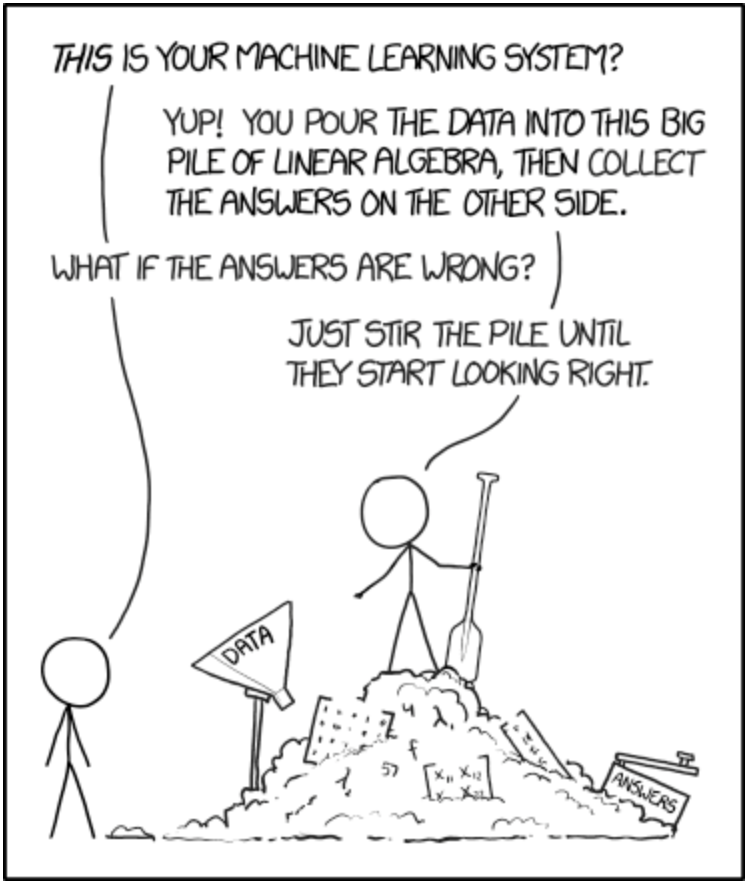
\includegraphics[scale=0.45]{Graphics/ml.png}
\end{savequote}
\chapter{Systems of Linear Equations}

    \section{Lecture 6: September 2, 2022}

    \subsection{Systems of Linear Equations}
    
        Consider the following definitions.
        \begin{definition}{\Stop\,\,Linear Equations}{lineq}
        
            A linear equation is an equation of the form 
            \begin{equation*}
                a_1x_1+\cdots+a_nx_n=b.
            \end{equation*}
            
        \end{definition}
        \begin{definition}{\Stop\,\,Systems of Linear Equations}{syslineq}
        
            A system of linear equations is a system of the form 
            \begin{align*}
                a_{11}x_1+\cdots+a_{1n}x_n&=b_1 \\
                &\vdots \\
                a_{m1}x_1+\cdots+a_{mn}x_n&=b_m.
            \end{align*}
            
        \end{definition}
        \pagebreak
        
\pagebreak
        
\section{Lecture 7: September 7, 2022}

    \subsection{Systems of Linear Equations as Matrices}

        We may write systems of linear equations in terms of matrices as
        \begin{equation*}
            A\begin{bmatrix} x_1 \\ \vdots \\ x_n \end{bmatrix}=\begin{bmatrix} b_1 \\ \vdots \\ b_m \end{bmatrix},
        \end{equation*}
        where \(A\) is the matrix with entries \(a_{ij}\). Consider the following theorem.
        \begin{theorem}{\Stop\,\,Characterizing Solutions of Linear Systems}{charsollinsys}
            
            A system of linear equations can either have
            \begin{enumerate}
                \item No solution.
                \item One unique solution.
                \item Infinitely many solutions.
            \end{enumerate}
            
        \end{theorem}

    \subsection{Matrix Row Operations}
    
        Consider the following operations.
        \begin{enumerate}
            \item Multiplication of a row by a nonzero scalar. Notated as \(c\langle r_1\rangle\to\langle r_1\rangle\).
            \item Addition of a scalar multiple of one row to another. Notated as \(\langle r_1\rangle +(c)\langle r_2\rangle\to\langle r_1\rangle\)
            \item Switching the elements of two rows. Notated as \(\langle r_1 \rangle \leftrightarrow \langle r_2 \rangle\).
        \end{enumerate}
        \vphantom
        \\
        \\
        Consider the following examples.
        \begin{example}{\Difficulty\,\Difficulty\,\,Row Operation 1}{rowop1}
        
            Consider the matrix \(\begin{bmatrix} 3 & 1 & -1 \\ 1 & 0 & 1 \\ -1 & 1 & 5 \end{bmatrix}\). Find \(4\langle 3\rangle\to\langle 3\rangle\).
            \\
            \\
            We obtain
            \begin{equation*}
                \begin{bmatrix}
                    3 & 1 & -1 \\
                    1 & 0 & 1 \\
                    -4 & 4 & 20
                \end{bmatrix}.
            \end{equation*}
    
        \end{example}
        \pagebreak
        \begin{example}{\Difficulty\,\Difficulty\,\,Row Operation 2}{rowop2}
        
            Consider the matrix \(\begin{bmatrix} 3 & 1 & -1 \\ 1 & 0 & 1 \\ -1 & 1 & 5 \end{bmatrix}\). Find \(\langle 1\rangle +(-3)\langle 2\rangle\to\langle 1\rangle\).
            \\
            \\
            We obtain
            \begin{equation*}
                \begin{bmatrix}
                    0 & 1 & -4 \\
                    1 & 0 & 1 \\
                    -1 & 1 & 5
                \end{bmatrix}.
            \end{equation*}
        \end{example}
        \begin{example}{\Difficulty\,\Difficulty\,\,Row Operation 3}{rowop3}
        
            Consider the matrix \(\begin{bmatrix} 3 & 1 & -1 \\ 1 & 0 & 1 \\ -1 & 1 & 5 \end{bmatrix}\). Find \(\langle 2\rangle\leftrightarrow\langle 3\rangle\).
            \\
            \\
            We obtain
            \begin{equation*}
                \begin{bmatrix}
                    3 & 1 & -1 \\
                    -1 & 1 & 5 \\
                    1 & 0 & 1
                \end{bmatrix}.
            \end{equation*}
    
        \end{example}
        
\pagebreak
        
\section{Lecture 8: September 9, 2022}

    \subsection{Solving Linear Systems}
    
        Given a linear system of equations, we solve by the following steps.
        \begin{enumerate}
            \item Convert the linear system into the matrix equation \(AX=B\), written \([A|B]\).
            \item Use the three row operations to reduce \([A|B]\) to one with ``lots of zeroes and ones.''
            \item Perform back substitution and analyze the solution set.
        \end{enumerate}
        \vphantom
        \\
        \\
        Consider the following examples.
        \begin{example}{\Difficulty\,\Difficulty\,\,No Solution}{nosols}
            
            Consider the matrix
            \begin{equation*}
                \begin{bmatrix} 
                3 & -6 & 0 & 3 & | & 9 \\
                -2 & 4 & 2 & -1 & | & -11 \\
                4 & -8 & 6 & 7 & | & -5
                \end{bmatrix}.
            \end{equation*}
            By row operations, we obtain
            \begin{equation*}
                \begin{bmatrix} 
                1 & -2 & 0 & 1 & | & 3 \\
                0 & 0 & 1 & \frac{1}{2} & | & -\frac{5}{2} \\
                0 & 0 & 0 & 0 & | & -2
                \end{bmatrix}.
            \end{equation*}
            Looking at the last row, we see the equation \(0=-2\), which is not true. Hence, the system has no solution.
            
        \end{example}
        \begin{example}{\Difficulty\,\Difficulty\,\,Infinitely Many Solutions}{infmanysols}
            
            Consider the matrix
            \begin{equation*}
                \begin{bmatrix} 
                3 & 1 & 7 & 2 & | & 13 \\
                2 & -4 & 14 & -1 & | & -10 \\
                5 & 11 & -7 & 8 & | & 59 \\
                2 & 5 & -4 & -3 & | & 39
                \end{bmatrix}.
            \end{equation*}
            By row operations, we obtain
            \begin{equation*}
                \begin{bmatrix} 
                1 & \frac{1}{3} & \frac{7}{3} & \frac{2}{3} & | & \frac{13}{3} \\
                0 & 1 & -2 & \frac{1}{2} & | & 4 \\
                0 & 0 & 0 & 1 & | & 59 \\
                0 & 0 & 0 & 0 & | & 0
                \end{bmatrix}.
            \end{equation*}
            We see that \(x_1\), \(x_2\), and \(x_4\) are determined because their respective column has a \(1\) in the correct position. In contrast, \(x_3\) is a free variable. To find the solution set, let \(x_3=c\in\mathbb{R}\) and solve for \(x_1\), \(x_2\), and \(x_4\) in terms of \(c\). We have \(x_4=-2\). Then to find \(x_2\) we have
            \begin{equation*}
                x_2-2x_3+\frac{1}{2}x_4=4\implies x_2-2+\frac{1}{2}(-2)=4\implies x_2=2c+5.
            \end{equation*}
            For \(x_1\), we have
            \begin{equation*}
                x_1+\frac{1}{3}x_2+\frac{7}{3}x_3+\frac{2}{3}x_4=\frac{13}{3}\implies x_1=-3c+4.
            \end{equation*}
            The solution set is then \(\{(-3c+4,2c+5,c,-2):c\in\mathbb{R}\}\).
        \end{example}
        \vphantom
        \\
        \\
        We generally agree that back substitution is not much fun. Consider the following example.
        \begin{example}{\Difficulty\,\Difficulty\,\,No More Back Substitution}{nomorebacksub}
            Note that the matrix 
            \begin{equation*}
                \begin{bmatrix} 3 & -3 & -2 &| &23 \\ -6 & 4 & 3 &| &-40 \\ -2 & 1 & 1 &| &-12 \end{bmatrix}
            \end{equation*}
            reduces into
            \begin{equation*}
                \begin{bmatrix} 1 & -1 & -\frac{2}{3} &| &\frac{23}{3} \\ 0 & 1 & \frac{1}{3} &| &-\frac{10}{3} \\ 0 & 0 & 1 &| &2 \end{bmatrix}.
            \end{equation*}
            We may now ``get rid of'' \(-1\), \(-\frac{2}{3}\), and \(\frac{1}{3}\). We perform \(-\frac{1}{3}\langle 3\rangle+\langle 2\rangle\to\langle2\rangle\) which produces
            \begin{equation*}
                \begin{bmatrix} 1 & -1 & -\frac{2}{3} &| &\frac{23}{3} \\ 0 & 1 & 0 &| & -4 \\ 0 & 0 & 1 & | & 2 \end{bmatrix}.
            \end{equation*}
            Then, we will perform \(\langle 1\rangle + \langle 2\rangle\to\langle1\rangle\), yielding
            \begin{equation*}
                \begin{bmatrix} 1 & 0 & -\frac{2}{3} &| & \frac{23}{3}-4 \\ 0 & 1 & 0 &| & -4 \\ 0 & 0 & 1 & | & 2 \end{bmatrix}.
            \end{equation*}
            Finally, we will perform \(\frac{2}{3}\langle3\rangle+\langle1\rangle\to 1\), obtaining
            \begin{equation*}
                \begin{bmatrix}
                1 & 0 & 0 & | & 5 \\
                0 & 1 & 0 & | & -4 \\
                0 & 0 & 1 & | & 2
            \end{bmatrix}
            \end{equation*}
            which means \(x_1=5\), \(x_2=-4\), and \(x_3=2\).
        \end{example}
        \vphantom
        \\
        \\
        Consider the following theorem.
        \begin{theorem}{\Stop\,\,Row Operations}{rowops}
        
            Suppose \(A\in\mathcal{M}_{mn}\) and \(B\in\mathcal{M}_{np}\). Then,
            \begin{enumerate}
                \item If \(R\) is a row operation, \(R(AB)=(R(A))B\).
                \item If \(R_1,\ldots,R_n\) are row operations, \(R_n(
                \ldots(R_2(R_1(AB)))\ldots)=(R_n(\ldots(R_2(R_1(A)))\ldots))B\).
            \end{enumerate}
            \begin{proof}
                For \((1)\), see Assignment 2, Question 2 for the relationship between matrix multiplication and row operations. For \((2)\), use induction on \(k\).
            \end{proof}
            \DOTHISLATER
        \end{theorem}
        
    \pagebreak
    \vphantom
    \\
    \\
    Consider the following examples of solving linear systems.
    \begin{example}{\Difficulty\,\Difficulty\,\,Linear System 1}{linsys1}
        Solve the following system:
        \begin{equation*}
            \begin{bmatrix}
                2 & -1 & 1 & | & 0 \\
                1 & 3 & 4 & | & 0
            \end{bmatrix}
        \end{equation*}
        We first perform the row operation \(\frac{1}{2}\langle 1\rangle\to\langle 1\rangle\), which produces
        \begin{equation*}
            \begin{bmatrix}
                1 & -\frac{1}{2} & \frac{1}{2} & | & 0 \\
                1 & 3 & 4 & | & 0
            \end{bmatrix}.
        \end{equation*}
        Then, we perform \(\langle 1\rangle -\langle 2\rangle\to\langle 2\rangle\). We obtain
        \begin{equation*}
            \begin{bmatrix}
                1 & -\frac{1}{2} & \frac{1}{2} & | & 0 \\
                0 & -\frac{7}{2} & -\frac{7}{2} & | & 0
            \end{bmatrix}.
        \end{equation*}
        Next, we have \(-\frac{2}{7}\langle 2\rangle\to\langle 2\rangle\). This yields
        \begin{equation*}
            \begin{bmatrix}
                1 & -\frac{1}{2} & \frac{1}{2} & | & 0 \\
                0 & 1 & 1 & | & 0
            \end{bmatrix}. 
        \end{equation*}
        From here, let \(x_3=c\). Then, \(x_2=-c\). To find \(x_1\), we use the equation 
        \begin{equation*}
            x_1-\frac{1}{2}(-c)+\frac{1}{2}c=0,
        \end{equation*}
        which implies that \(x_1=-c\). Thus, the solution set is \(\{(-c,-c,c):c\in\mathbb{R}\}\).
    \end{example}
    \pagebreak
    \begin{example}{\Difficulty\,\Difficulty\,\,Linear System 2}{linsys2}
        Solve the following system:
        \begin{equation*}
            \begin{bmatrix}
                1 & -2 & 1 & 2 & | & 1 \\
                1 & 1 & -1 & 1 & | & 2 \\
                1 & 7 & -5 & -1 & | & 3
            \end{bmatrix}
        \end{equation*}
        First, we perform \(\langle 1\rangle -\langle 2\rangle\to\langle 2\rangle\), yielding
        \begin{equation*}
            \begin{bmatrix}
                1 & -2 & 1 & 2 & | & 1 \\
                0 & -3 & 2 & 1 & | & -1 \\
                1 & 7 & -5 & -1 & | & 3
            \end{bmatrix}.
        \end{equation*}
        Then, we perform \(\langle 1\rangle-\langle 3\rangle\to\langle 3\rangle\). We obtain
        \begin{equation*}
            \begin{bmatrix}
                1 & -2 & 1 & 2 & | & 1 \\
                0 & -3 & 2 & 1 & | & -1 \\
                0 & -9 & 6 & 3 & | & -2 
            \end{bmatrix}.
        \end{equation*}
        Then, we have \(-\frac{1}{3}\langle 2\rangle\to\langle 2\rangle\). This produces
        \begin{equation*}
            \begin{bmatrix}
                1 & -2 & 1 & 2 & | & 1 \\
                0 & 1 & -\frac{2}{3} & -\frac{1}{3} & | & \frac{1}{3} \\
                0 & -9 & 6 & 3 & | & -2
            \end{bmatrix}.
        \end{equation*}
        Our final row operation is \(\langle3\rangle+9\langle2\rangle\to\langle 3\rangle\). This provides us with
        \begin{equation*}
            \begin{bmatrix}
                 1 & -2 & 1 & 2 & | & 1 \\
                 0 & 1 & -\frac{2}{3} & -\frac{1}{3} & | & \frac{1}{3} \\
                 0 & 0 & 0 & 0 & | & 1
            \end{bmatrix},
        \end{equation*}
        meaning that there is no solution to the system.
    \end{example}
    \pagebreak
    \begin{example}{\Difficulty\,\Difficulty\,\,Linear System 3}{linsys3}
        Solve the following system:
        \begin{equation*}
            \begin{bmatrix}
                 1 & -1 & 2 & | & 1 \\
                 2 & 0 & 2 & | & 1 \\
                 1 & -3 & 4 & | & 2
            \end{bmatrix}
        \end{equation*}
        Our first row operation is \(2\langle1\rangle-\langle2\rangle\to\langle2\rangle\). This produces
        \begin{equation*}
            \begin{bmatrix}
                 1 & -1 & 2 & | & 1 \\
                 0 & -2 & 2 & | & 1 \\
                 1 & -3 & 4 & | & 2
            \end{bmatrix}.
        \end{equation*}
        Then, we have \(\langle1\rangle-\langle3\rangle\to\langle3\rangle\), providing
        \begin{equation*}
            \begin{bmatrix}
                 1 & -1 & 2 & | & 1 \\
                 0 & -2 & 2 & | & 1 \\
                 0 & 2 & -2 & | & -1
            \end{bmatrix}.
        \end{equation*}
        Next, we perform \(\langle2\rangle+\langle3\rangle\to\langle3\rangle\). We obtain
        \begin{equation*}
            \begin{bmatrix}
                 1 & -1 & 2 & | & 1 \\
                 0 & -2 & 2 & | & 1 \\
                 0 & 0 & 0 & | & 0
            \end{bmatrix}.
        \end{equation*}
        We perform another row operation, \(-\frac{1}{2}\langle 2\rangle\to\langle 2\rangle\). This yields
        \begin{equation*}
            \begin{bmatrix}
                 1 & -1 & 2 & | & 1 \\
                 0 & 1 & -1 & | & -\frac{1}{2} \\
                 0 & 0 & 0 & | & 0
            \end{bmatrix}.
        \end{equation*}
        Next, we have \(\langle2\rangle+\langle1\rangle\to\langle1\rangle\), which gives
        \begin{equation*}
            \begin{bmatrix}
                 1 & 0 & 1 & | & \frac{1}{2} \\
                 0 & 1 & -1 & | & -\frac{1}{2} \\
                 0 & 0 & 0 & | & 0
            \end{bmatrix}.
        \end{equation*}
        Let \(x_3=c\). Then, \(x_2=-\frac{1}{2}+c\) and \(x_1=\frac{1}{2}-c\). This means the solution set is \(\{\left(\frac{1}{2}-c,-\frac{1}{2}+c,c\right):c\in\mathbb{R}\}\).
    \end{example}

\pagebreak

\section{Lecture 9: September 12, 2022}

    \subsection{Formalizing Previous Notions Part I}

    Consider the following definitions.
    \begin{definition}{\Stop\,\,Row Echelon Form}{rowechelon}
        
        A matrix \(A\) is in row echelon form if and only if
        \begin{enumerate}
            \item All rows consisting of only zeroes are at the bottom.
            \item The leading coefficient, or the pivot, of a nonzero row is always strictly to the right of the leading coefficient of the row above it.
        \end{enumerate}
    
    \end{definition}
    \begin{definition}{\Stop\,\,Reduced Row Echelon Form}{redrowechelon}
    
        A matrix \(A\) is in reduced row echelon form if and only if
        \begin{enumerate}
            \item The first nonzero entry in each row is one.
            \item Each successive row has its first nonzero entry in a later column.
            \item All entries above and below the first nonzero entry are zero.
            \item All rows consisting of only zeroes are at the bottom.
        \end{enumerate}
        
    \end{definition}
    \vphantom
    \\
    \\
    Note that every matrix has a unique reduced row echelon form.
    \\
    \\
    Consider the following theorems and definitions.
    \begin{theorem}{\Stop\,\,Number of Solutions to a Linear System}{numsollinsys}
    
        Let \(AX=B\) be a system of linear equations. Let \(C\) be the reduced row echelon form augmented matrix obtained by row reducing \([A|B]\). Then,
        \begin{enumerate}
            \item If there is a row of \(C\) having all zeroes to the left of the augmentation bar but with its last entry nonzero, \(AX=B\) has no solution.
            \item If not, and if one of the columns of \(C\) to the left of the augmentation bar has no nonzero pivot entry, \(AX=B\) has an infinite number of solutions. The nonpivot columns correspond to (independent) variables that can take on any value, and the values of the remaining (dependent) variables are determined from those.
            \item Otherwise \(AX=B\) has a unique solution.
        \end{enumerate}
    
    \end{theorem}
    \pagebreak
    \vphantom
    \\
    \\
    Consider the following definitions.
    \begin{definition}{\Stop\,\,Homogeneous Systems}{homosys}
    
        Given \(A\in\mathcal{M}_{mn}\), the homogeneous system associated with \(A\) is
        \begin{equation*}
            AX=\begin{bmatrix}
            0 \\
            \vdots \\
            0
            \end{bmatrix}.
        \end{equation*}
    
    \end{definition}
    \begin{theorem}{\Stop\,\,Solutions to Homogeneous Systems}{solstohomosys}
    
        Given \(A\in\mathcal{M}_{mn}\), the homogeneous system always has at least one solution, called the \textit{trivial solution}. Namely,
        \begin{equation*}
            x_1=0,\quad x_2=0,\quad\ldots,\quad x_n=0.
        \end{equation*}
        Also, consider the following.
        \begin{enumerate}
            \item If \(m<n\), the solution set is infinite. 
            \item If \(X=\begin{bmatrix} x_1 \\ \vdots \\ x_n \end{bmatrix}\) and \(X_\sim=\begin{bmatrix} x_{\sim 1} \\ \vdots \\ x_{\sim n} \end{bmatrix}\) are solutions,
            \begin{equation*}
                cX+X_\sim
            \end{equation*}
            is a solution for any \(c\in\mathbb{R}\).
            \item If \(AX=\begin{bmatrix} 0 \\ \vdots \\ 0 \end{bmatrix}\) and \(A\hat{X}=B=\begin{bmatrix} b_1 \\ \vdots \\ b_m \end{bmatrix}\),
            \begin{equation*}
                cX+\hat{X}
            \end{equation*}
            is a solution to \([A|B]\). Notice that (2) is a special case of (3).
            \begin{proof}
                Consider \(A(cX+\hat{X})\). We wish to show that \(A(cX+\hat{X})=B\). We see that
                \begin{align*}
                    A(cX+\hat{X})&=A(cX)+A\hat{X} \\
                    &=cAX+A\hat{X} \\
                    &=\begin{bmatrix} 0 \\ \vdots \\ 0 \end{bmatrix}+\begin{bmatrix} b_1 \\ \vdots \\ b_m \end{bmatrix} \\
                    &=B,
                \end{align*}
                as desired.
            \end{proof}
            This process is analogous to solving homogeneous differential equations to solve nonhomogeneous differential equations.
        \end{enumerate}
    
    \end{theorem}
    \begin{definition}{\Stop\,\,Equivalence of Linear Systems}{sysequiv}
        Two systems \([A|B]\) and \([A_\sim|B_\sim]\) are equivalent if and only if
        \begin{equation*}
            AX=B\wedge A_\sim X=B_\sim.
        \end{equation*}
        That is, if they have the same solution sets.
    \end{definition}
    \begin{definition}{\Stop\,\,Row Equivalence}{rowequiv}
        A matrix \(A\) is row equivalent to a matrix \(B\) if \(B\) can be obtained by a finite number of row operations conducted on \(A\).
    \end{definition}
    \vphantom
    \\
    \\
    For example, Gaussian Elimination and Gauss-Jordan Elimination produce matrices that are row equivalent to the original matrix.
    \\
    \\
    One may ask: What is the relationship between these relations? We see that row equivalence implies system equivalence. But, two systems can have the same solution set, but have different sizes, making row equivalence impossible. For the latter case, consider two matrices of different sizes, but with an empty solution set. Recall from discrete mathematics,
    \begin{definition}{\Stop\,\,Equivalence Relations}{equivrel}
        
        A relation \(\sim\) on a set \(S\) is an equivalence relation on \(S\) if and only if \(\sim\) is reflexive, symmetric, and transitive. That is, if
        \begin{enumerate}
            \item \(\forall a\in S, a\sim a\).
            \item \(\forall a, b\in S, a\sim b\implies b\sim a\)
            \item \(\forall a, b, c\in S, a\sim b\wedge b\sim c\implies a\sim c\).
        \end{enumerate}
        
    \end{definition}
    \pagebreak
    \vphantom
    \\
    \\
    Consider the following theorem.
    \begin{theorem}{\Stop\,\,System Equivalence and Row Equivalence are Equivalence Relations}{equivrelrowsysequiv}
    
        First, consider the following table.
        \begin{center}
            \begin{tabular}{c|c}
                \hline
                Row Operation & Reverse Operation \\
                \hline
                \(c\langle i\rangle \to \langle i\rangle\) & \(\frac{1}{c}\langle i\rangle \to \langle i \rangle\) \\
                \(c\langle i \rangle+\langle j \rangle \to\langle j\rangle\) & \(-c\langle i \rangle+\langle j \rangle\to\langle j \rangle\) \\
                \(\langle i \rangle \leftrightarrow \langle j \rangle\) & \(\langle i \rangle \leftrightarrow \langle j \rangle\) \\
                \hline
            \end{tabular}
        \end{center}
        \vphantom
        \\
        \\
        \begin{proof}
            We will consider row equivalence first, and wish to show that row equivalence is reflexive, symmetric, and transitive. Reflexivity is trivial. We can simply not perform any row operations on a matrix \(A\), and we are left with \(A\). The above table can be used to show that row equivalence is symmetric. If a sequence of row operations is carried out on \(A\) and produces a matrix \(B\), we can simply carry out the reverse operations on \(B\) to lead us back to \(A\). For transitivity, if a sequence of row operations is carried out on \(A\) and leads to \(B\), and a second sequence of row operations is performed on \(B\) and leads to \(C\), we simply carry out the sequences, in sequence, on \(A\) to get us to \(C\).
            \\
            \\
            Now, we consider system equivalence. The system \([A|B]\), of course, has the same solution set as itself. If the system \([A|B]\) has the same solution set as \([C|D]\), \([C|D]\) has the same solution set as \([A|B]\). If \([A|B]\) has the same solution set as \([C|D]\) and \([C|D]\) has the same solution set as the system \([E|F]\), \([A|B]\) has the same solution set as \([E|F]\).
        \end{proof}
        
    \end{theorem}

\pagebreak

\section{Lecture 10: September 14, 2022}

    \subsection{Formalizing Previous Notions Part II}
    
        Consider the following formalization of our last discoveries.
        \begin{theorem}{\Stop\,\,Row Equivalence Implies System Equivalence}{rowsyseq}
        
            If \([A|B]\) is equivalent to \([C|D]\), \([A|B]\) is equivalent to \([C|D]\). We assume that 
            \begin{equation*}
                R_n(R_{n-1}(\ldots R_1([A|B]))\ldots)
            \end{equation*}
            We will use induction on \(n\). The base case is \(R_1([A|B])=[C|D]\). There are three cases,
            \begin{enumerate}
                \item \(R_1\) is \(c\langle i\rangle\to\langle i\rangle\).
                    We have that \(R_1\) is \(c\langle i \rangle \to \langle i \rangle\) for \(c\neq0\). The system has the form
                    \begin{align*}
                        a_{11}x_1+\cdots+a_{1n}x_n&=b_1 \\
                        &\vdots \\
                        a_{i1}x_1+\cdots+a_{in}x_n&=b_i \\
                        &\vdots \\
                        a_{m1}x_1+\cdots+a_{mn}x_n&=b_m.
                    \end{align*}
                    After \(c\langle i \rangle \to \langle i \rangle\), the system is
                    \begin{align*}
                        a_{11}x_1+\cdots+a_{1n}x_n&=b_1 \\
                        &\vdots \\
                        ca_{i1}x_1+\cdots+ca_{in}x_n&=cb_i \\
                        &\vdots \\
                        a_{m1}x_1+\cdots+a_{mn}x_n&=b_m.
                    \end{align*}
                    We see that the solution sets are the same. The first and third rows are the same, so the solution sets will be the same. For the second row, simply factor by \(c\) and divide.
                \item \(R_1\) is \(\langle c\rangle\langle j \rangle+\langle i\rangle\to \langle i\rangle\).
                \item \(R_1\) is \(\langle i \rangle \leftrightarrow \langle j\rangle\).
            \end{enumerate}
            \vphantom
            \\
            \\
            The proposition for \(n=k\) is,
            \begin{equation*}
                R_k(R_{k-1}(\ldots R_1([A|B]))\ldots)
            \end{equation*}
            has the same solution as \([A|B]\), but
            \begin{equation*}
                R_{k+1}(R_k(R_{k-1}(\ldots R_1([A|B]))\ldots)
            \end{equation*}
            has the same solution as
            \begin{equation*}
                R_k(R_{k-1}(\ldots R_1([A|B]))\ldots).
            \end{equation*}
            Thus, 
            \begin{equation*}
                R_{k+1}(R_k(R_{k-1}(\ldots R_1([A|B]))\ldots)
            \end{equation*}
            has the same solution set as \([A|B]\).
        \end{theorem}
        \begin{theorem}{\Stop\,\,Uniqueness of Reduced Row Echelon Form}{uniquenessredrow}
        
            Every matrix is row equivalent to a unique matrix in reduced row echelon form. Two matrices are row equivalent if and only if they have the same reduced row echelon form.
            
        \end{theorem}
        \begin{definition}{\Stop\,\,Rank}{rank}
        
            Given \(A\in\mathcal{M}_{mn}\), \(\rank{A}\) is the number of nonzero rows in the unique matrix that is row equivalent to \(A\) and is in reduced row echelon form.
            
        \end{definition}
        \vphantom
        \\
        \\
        Consider the following example.
        \begin{example}{\Difficulty\,\Difficulty\,\,Rank 1}{rank1}
        
            Consider
            \begin{equation*}
                A=\begin{bmatrix}
                3 & 1 & 0 & 1 \\
                0 & -2 & 12 & -5 \\
                2 & -3 & 22 & -14
                \end{bmatrix}.
            \end{equation*}
            By row reduction, we have the matrix
            \begin{equation*}
                \begin{bmatrix}
                1 & 0 & 2 & -1 \\
                0 & 1 & -6 & 4 \\
                0 & 0 & 0 & 0
                \end{bmatrix},
            \end{equation*}
            and see that \(\rank A=2\).
        \end{example}
        \vphantom
        \\
        \\
        Consider the following theorem. 
        \begin{theorem}{\Stop\,\,Number of Solutions to Homogeneous Systems}{numsolshomosys}
        
            If \(A\in\mathcal{M}_{mn}\),
            \begin{enumerate}
                \item If \(\rank A< n\), \(AX=0\) has an infinite solution set.
                \item If \(\rank A= n\), \(AX=0\) has only the trivial solution.
            \end{enumerate}
        
        \end{theorem}
        \vphantom
        \\
        \\
        We will now define linear combinations of vectors.
        \begin{definition}{\Stop\,\,Linear Combinations}{lincomb}
    
            Let \(\vec{v}_1,\vec{v}_2,\ldots,\vec{v}_k\in\mathbb{R}^n\). The vector \(\vec{v}\) is a linear combination of \(\vec{v}_1,\vec{v}_2,\ldots,\vec{v}_k\) if and only if there are scalars \(c_1,c_2,\ldots,c_k\) such that 
            \begin{equation*}
                \vec{v}=c_1\vec{v}_1+\cdots+c_k\vec{v}_k.
            \end{equation*}
            
        \end{definition}
        \vphantom
        \\
        \\
        In general, \(\{c\vec{v}:c\in\mathbb{R}\}\) is a line unless \(\vec{v}=\vec{0}\). Also, \(\{c_1\vec{v}_1+c_2\vec{v}_2:c_1,c_2\in\mathbb{R}\}\) is usually a plane, but could be either a point or a line. This pattern is an introduction to the concept of linear dependence, which will be elaborated on later in the text.
        \pagebreak
        \vphantom
        \\
        \\
        Consider the following example.
        \begin{example}{\Difficulty\,\Difficulty\,\,Is a Vector a Linear Combination of Others? 1}{veclincombothers1}
        
            Let \(\vec{v}=[1,0]\), \(\vec{v}_1=[\pi,1]\), and \(\vec{v}_2=[2,1]\). Is \(\vec{v}\) a linear combination of \(\vec{v}_1\) and \(\vec{v}_2\)?
            \\
            \\
            Notice that \(\vec{v}_1-\vec{v}_2=[\pi-2,0]\). Then,
            \begin{equation*}
                \frac{1}{\pi-2}[\pi-2,0]=[1,0]=\vec{v}.
            \end{equation*}
            We then have that
            \begin{equation*}
                \vec{v}=\frac{1}{\pi-2}[\pi,1]-\frac{1}{\pi-2}[2,1].
            \end{equation*}
            Therefore, \(\vec{v}\) is a linear combination of \(\vec{v}_1\) and \(\vec{v}_2\).
        \end{example}
        \vphantom
        \\
        \\
        The above solution used a bit of trickery. Instead, given \(\vec{v}_1,\ldots,\vec{v}_k\), we form the equation
        \begin{equation*}
            \begin{bmatrix}
                \vec{v}_1,\ldots,\vec{v}_k
            \end{bmatrix}
            \begin{bmatrix}
                c_1 \\ \vdots \\ c_k
            \end{bmatrix}
            =\begin{bmatrix} \vec{v} \end{bmatrix}
        \end{equation*}
        and solve for the necessary constants.
        \pagebreak
        \\
        \\
        Consider the following examples.
        \begin{example}{\Difficulty\,\Difficulty\,\,Is a Vector a Linear Combination of Others? 2}{veclincombothers2}
        
            Let \(\vec{v}=[1,0,0]\), \(\vec{v}_1=[-4,2,0]\), and \(\vec{v}_2=[2,1,1]\). Is \(\vec{v}\) a linear combination of \(\vec{v}_1\) and \(\vec{v}_2\)?
            \\
            \\
            Consider the system
            \begin{equation*}
                \begin{bmatrix}
                    -4 & 2 & | & 1 \\
                    2 & 1 & | & 0 \\
                    0 & 1 & | & 0
                \end{bmatrix}.
            \end{equation*}
            We first perform the row operation \(-\frac{1}{4}\langle1\rangle\to\langle1\rangle\) to obtain
            \begin{equation*}
                \begin{bmatrix}
                    1 & -\frac{1}{2} & | & -\frac{1}{4} \\
                    2 & 1 & | & 0 \\
                    0 & 1 & | & 0
                \end{bmatrix}.
            \end{equation*}
            Then, we have \(2\langle1\rangle-\langle2\rangle\to\langle2\rangle\), producing
            \begin{equation*}
                \begin{bmatrix}
                    1 & -\frac{1}{2} & | & -\frac{1}{4} \\
                    0 & -2 & | & -\frac{1}{2} \\
                    0 & 1 & | & 0
                \end{bmatrix}.
            \end{equation*}
            Next, we will carry out \(-\frac{1}{2}\langle2\rangle\to\langle2\rangle\) to yield
            \begin{equation*}
                \begin{bmatrix}
                    1 & -\frac{1}{2} & | & -\frac{1}{4} \\
                    0 & 1 & | & \frac{1}{4} \\
                    0 & 1 & | & 0
                \end{bmatrix}.
            \end{equation*}
            We will then compute \(\langle2\rangle-\langle3\rangle\to\langle3\rangle\); we have
            \begin{equation*}
                \begin{bmatrix}
                    1 & -\frac{1}{2} & | & -\frac{1}{4} \\
                    0 & 1 & | & \frac{1}{4} \\
                    0 & 0 & | & \frac{1}{4}
                \end{bmatrix}.
            \end{equation*}
            There is no solution, so \(\vec{v}\) is not a linear combination of \(\vec{v}_1\) and \(\vec{v}_2\).
            
        \end{example}
        \pagebreak
        \begin{example}{\Difficulty\,\Difficulty\,\,Is a Vector a Linear Combination of Others? 3}{veclincombothers3}
        
            Let \(\vec{v}=[14,-21,7]\), \(\vec{v}_1=[2,-3,1]\), and \(\vec{v}_2=[-4,6,2]\). Is \(\vec{v}\) a linear combination of \(\vec{v}_1\) and \(\vec{v}_2\)?
            \\
            \\
            Consider the system
            \begin{equation*}
                \begin{bmatrix}
                    2 & -4 & | & 14 \\
                    -3 & 6 & | & -21 \\
                    1 & 2 & | & 7
                \end{bmatrix}.
            \end{equation*}
            We first perform the row operation \(\frac{1}{2}\langle1\rangle\to\langle1\rangle\) to obtain
            \begin{equation*}
                \begin{bmatrix}
                    1 & -2 & | & 7 \\
                    -3 & 6 & | & -21 \\
                    1 & 2 & | & 7
                \end{bmatrix}.
            \end{equation*}
            Then, we have \(3\langle1\rangle+\langle2\rangle\to\langle2\rangle\), producing
            \begin{equation*}
                \begin{bmatrix}
                    1 & -2 & | & 7 \\
                    0 & 0 & | & 0 \\
                    1 & 2 & | & 7
                \end{bmatrix}.
            \end{equation*}
            Next, we will carry out \(\langle2\rangle\leftrightarrow\langle3\rangle\) to yield
            \begin{equation*}
                \begin{bmatrix}
                    1 & -2 & | & 7 \\
                    1 & 2 & | & 7 \\
                    0 & 0 & | & 0
                \end{bmatrix}.
            \end{equation*}
            We will then compute \(\langle1\rangle+\langle2\rangle\to\langle2\rangle\); we have
            \begin{equation*}
                \begin{bmatrix}
                    1 & -2 & | & 7 \\
                    2 & 0 & | & 14 \\
                    0 & 0 & | & 0
                \end{bmatrix}.
            \end{equation*}
            Then, we will execute \(2\langle1\rangle-\langle2\rangle\to\langle2\rangle\), and we obtain
            \begin{equation*}
                \begin{bmatrix}
                    1 & -2 & | & 7 \\
                    0 & -4 & | & 0 \\
                    0 & 0 & | & 0
                \end{bmatrix}.
            \end{equation*}
            We then have, by \(-\frac{1}{4}\langle2\rangle\to\langle2\rangle\),
            \begin{equation*}
                \begin{bmatrix}
                    1 & -2 & | & 7 \\
                    0 & 1 & | & 0 \\
                    0 & 0 & | & 0
                \end{bmatrix}.
            \end{equation*}
            Finally, we have the operation \(\langle1\rangle+2\langle2\rangle\to\langle1\rangle\), which produces
            \begin{equation*}
                \begin{bmatrix}
                    1 & 0 & | & 7 \\
                    0 & 1 & | & 0 \\
                    0 & 0 & | & 0
                \end{bmatrix}.
            \end{equation*}
            Here, we see that \(\vec{v}=7\vec{v}_1\). We note that it would have been simple to conclude this based on the problem statement, but the method shown is the systematic algorithm for answering such questions.
            
        \end{example}
        \pagebreak
        \begin{example}{\Difficulty\,\Difficulty\,\,Is a Vector a Linear Combination of Others? 4}{veclincombothers4}
        
            Let \(\vec{v}=[14,-21,7]\), \(\vec{v}_1=[2,-3,1]\), and \(\vec{v}_2=[-4,6,-2]\). Is \(\vec{v}\) a linear combination of \(\vec{v}_1\) and \(\vec{v}_2\)?
            \\
            \\
            Consider the system
            \begin{equation*}
                \begin{bmatrix}
                    2 & -4 & | & 14 \\
                    -3 & 6 & | & -21 \\
                    1 & -2 & | & 7
                \end{bmatrix}.
            \end{equation*}
            By row reduction, we finally obtain
            \begin{equation*}
                \begin{bmatrix}
                    1 & -2 & | & 7 \\
                    0 & 0 & | & 0 \\
                    0 & 0 & | & 0
                \end{bmatrix}.
            \end{equation*}
            Here, the solution set is \(\{(2c+7,c):c\in\mathbb{R}\}\). There are thus infinitely many ways to express \(\vec{v}\) as a linear combination of \(\vec{v}_1\) and \(\vec{v}_2\).
            
        \end{example}
        \vphantom
        \\
        \\
        Consider the following definition.
        \begin{definition}{\Stop\,\,Row Space}{rowspace}
        
            Suppose \(A\in\mathcal{M}_{mn}\). The row space of \(A\) is the subset of \(\mathbb{R}^n\) consisting of the linear combinations of the rows of \(A\).
            
        \end{definition}
        \vphantom
        \\
        \\
        Consider the following examples.
        \begin{example}{\Difficulty\,\,Row Space 1}{rsp1}
        
            Consider
            \begin{equation*}
                A=\begin{bmatrix}
                    1 & 2 \\
                    5 & 10
                \end{bmatrix}.
            \end{equation*} 
            The row space of \(A\) is 
            \begin{equation*}
                 \{c_1[1,2]+c_2[5,10]:c_1,c_2\in\mathbb{R}\}.
            \end{equation*}
            In this case, the row space of \(A\) is a line. Generally, though, with two vectors, the row space will be a plane.
        \end{example}
        \begin{example}{\Difficulty\,\,Row Space 2}{rsp2}
        
            Consider
            \begin{equation*}
                A=\begin{bmatrix}
                    1 & 3 \\
                    5 & 10
                \end{bmatrix}.
            \end{equation*} 
            The row space of \(A\) is 
            \begin{equation*}
                 \{c_1[1,3]+c_2[5,10]:c_1,c_2\in\mathbb{R}\}.
            \end{equation*}
            In this case, the row space of \(A\) is a plane.
        \end{example}
        \pagebreak
        \vphantom
        \\
        \\
        To determine if a vector is in the row space of a matrix \(A\), we consider the system \([A^T|X]\). One may ask: why? Well, considering \(A\) instead of \(A^T\) would provide the wrong system of equations to solve. All we are doing when determining if a vector is in the row space of \(A\) is asking if the vector can be written as a linear combination of the rows of \(A\). Consider the following example.
        \begin{example}{\Difficulty\,\Difficulty\,\,Are Vectors in the Row Space?}{vecrowspace}
            Consider
            \begin{equation*}
                A=\begin{bmatrix}
                    1 & 2 \\
                    5 & 10
                \end{bmatrix}
            \end{equation*} 
            and recall that the row space of \(A\) is 
            \begin{equation*}
                 \{c_1[1,2]+c_2[5,10]:c_1,c_2\in\mathbb{R}\}.
            \end{equation*}
            Is \([3,6]\) in the row space of \(A\)? Is \([1,0]\) in the row space of \(A\)? We consider
            \begin{equation*}
            \begin{bmatrix}
                1 & 2 \\
                5 & 10
            \end{bmatrix}^T\begin{bmatrix} x_1 \\ x_2 \end{bmatrix} = \begin{bmatrix} b_1 \\ b_2 \end{bmatrix}.
        \end{equation*}
        For \([3,6]\), we have
        \begin{equation*}
            \begin{bmatrix}
                1 & 5 & | & 3 \\
                2 & 10 & | & 6
            \end{bmatrix},
        \end{equation*}
        which reduces to
        \begin{equation*}
            \begin{bmatrix}
                1 & 5 & | & 3 \\
                0 & 0 & | & 0
            \end{bmatrix}.
        \end{equation*}
        The system has (infinitely many) solutions, so \([3,6]\) is in the row space of \(A\). For \([1,0]\), we have
        \begin{equation*}
            \begin{bmatrix}
                1 & 5 & | & 1 \\
                2 & 10 & | & 0
            \end{bmatrix},
        \end{equation*}
        which reduces to
        \begin{equation*}
            \begin{bmatrix}
                1 & 5 & | & 1 \\
                0 & 0 & | & -2
            \end{bmatrix}.
        \end{equation*}
        The system has no solution, so \([1,0]\) is not in the row space of \(A\).
        \end{example}
        \pagebreak
        \vphantom
        \\
        \\
        Consider the following theorems.
        \begin{theorem}{\Stop\,\,Transitivity of Linear Combinations}{translincomb}
        
            Suppose that \(\vec{x}\) is a linear combination of \(\vec{q}_1,\ldots,\vec{q}_k\), and suppose also that each of \(\vec{q}_1,\ldots,\vec{q}_k\) is itself a linear combination of \(\vec{r}_1,\ldots,\vec{r}_l\). Then, \(\vec{x}\) is a linear combination of \(\vec{r}_1,\ldots,\vec{r}_l\).
            \begin{proof}
                Because \(\vec{x}\) is a linear combination of \(\vec{q}_1,\ldots,\vec{q}_k\), 
                \begin{equation*}
                    \vec{x}=c_1\vec{q}_1+\cdots+c_k\vec{q}_k
                \end{equation*}
                for \(c_1,\ldots,c_k\in\mathbb{R}\). Then, since each of \(\vec{q}_1,\ldots,\vec{q}_k\) can be written as a linear combination of \(\vec{r}_1,\ldots,\vec{r}_l\), there exist scalars \(d_{11},\ldots,d_{kl}\) such that
                \begin{align*}
                    \vec{q}_1&=d_{11}\vec{r}_1+d_{12}\vec{r}_2+\cdots+d_{1l}\vec{r}_l \\
                    \vec{q}_2&=d_{21}\vec{r}_1+d_{22}\vec{r}_2+\cdots+d_{2l}\vec{r}_l \\
                    &\vdots \\
                    \vec{q}_k&=d_{k1}\vec{r}_1+d_{k2}\vec{r}_2+\cdots+d_{kl}\vec{r}_l
                \end{align*}
                Then,
                \begin{align*}
                    \vec{x}&=c_1(d_{11}\vec{r}_1+d_{12}\vec{r}_2+\cdots+d_{1l}\vec{r}_l) \\
                    &\quad+c_2(d_{21}\vec{r}_1+d_{22}\vec{r}_2+\cdots+d_{2l}\vec{r}_l) \\
                    &\quad\,\,\,\vdots \\
                    &\quad+c_k(d_{k1}\vec{r}_1+d_{k2}\vec{r}_2+\cdots+d_{kl}\vec{r}_l) \\
                    &=(c_1d_{11}+c_2d_{21}+\cdots+c_kd_{k1})\vec{r}_1 \\
                    &\quad+(c_1d_{12}+c_2d_{22}+\cdots+c_kd_{k2})\vec{r}_2 \\
                    &\quad\,\,\,\vdots \\\
                    &\quad+(c_1d_{1l}+c_2d_{2l}+\cdots+c_kd_{kl})\vec{r}_l.
                \end{align*}
                We have just written \(\vec{x}\) as a linear combination of \(\vec{r}_1,\ldots,\vec{r}_l\).
            \end{proof}
            Note that this theorem may be rephrased as follows: If \(\vec{x}\) is in the row space of a matrix \(Q\) and each row of \(Q\) is in the row space of a matrix \(R\), \(\vec{x}\) is in the row space of \(R\).
        \end{theorem}
        \begin{theorem}{\Stop\,\,Row Equivalence Implies Equal Row Space}{rowequivequalrowspc}
            
            Suppose \(A\) and \(B\) are row equivalent. Then, the row space of \(A\) is equal to the row space of \(B\).
        
        \end{theorem}

\pagebreak

\section{Lecture 11: September 16, 2022}

    \subsection{Linear Maps}
    
        Consider the following definition.
        \begin{definition}{\Stop\,\,Linear Maps}{linmaps}
        
            Given \(A\in\mathcal{M}_{mn}\), we define
            \begin{align*}
                T_A&:\mathbb{R}^n\to\mathbb{R}^m \\
                &:\begin{bmatrix} x_1 \\ \vdots \\ x_n \end{bmatrix}\mapsto A\begin{bmatrix} x_1 \\ \vdots \\ x_n \end{bmatrix}.
            \end{align*}
            
        \end{definition}
        \vphantom
        \\
        \\
        Consider the following example.
        \begin{example}{\Difficulty\,\Difficulty\,\,Some Special Maps in \(\mathbb{R}^2\)}{specialmapsr2}
            
            Consider the following maps, and name them.
            \begin{enumerate}
                \item If \(A=\begin{bmatrix} 0 & 0 \\ 0 & 0 \end{bmatrix}\), \(T_A:\mathbb{R}^2\to\mathbb{R}^2\) is the zero map.
                \item If \(A=\begin{bmatrix} 1 & 0 \\ 0 & 1 \end{bmatrix}\), \(T_A:\mathbb{R}^2\to\mathbb{R}^2\) is the identity map.
                \item If \(A=\begin{bmatrix} 1 & 0 \\ 0 & 0 \end{bmatrix}\), \(T_A:\mathbb{R}^2\to\mathbb{R}^2\) is the projection onto the \(x\) axis.
                \item If \(A=\begin{bmatrix} 0 & 0 \\ 0 & 1 \end{bmatrix}\), \(T_A:\mathbb{R}^2\to\mathbb{R}^2\) is the projection onto the \(y\) axis.
            \end{enumerate}
            
        \end{example}

\pagebreak

\section{Lecture 12: September 19, 2022}

    \subsection{Inverses of Matrices}

        Consider the following definitions and theorems.
        \begin{definition}{\Stop\,\,Multiplicative Inverse of a Matrix}{inverse}

            Let \(A\in\mathcal{M}_{nn}\). Then, \(B\in\mathcal{M}_{nn}\) is a multipliative inverse of \(A\) if and only if 
            \begin{equation*}
                AB=BA=I_n.
            \end{equation*}
            
        \end{definition}
        \begin{theorem}{\Stop\,\,Inverse Commutativity}{invcommute}
            
            Let \(A,B\in\mathcal{M}_{nn}\). If either \(AB\) or \(BA\) equals \(I_n\), the other product also equals \(I_n\), and \(A\) and \(B\) are inverses of each other.
            
        \end{theorem}
        \begin{definition}{\Stop\,\,Singularity}{singularity}

            A matrix is \texttt{singular} if and only if it is square and does not have an inverse. A matrix is \textit{nonsingular} if and only if it is square and has an inverse.
            
        \end{definition}
        \begin{theorem}{\Stop\,\,Uniqueness of the Inverse}{uniquenessinv}

            If \(B\) and \(C\) are both inverses of \(A\in\mathcal{M}_{nn}\), \(B=C\).
            \begin{proof}
                    \(B=BI_n=B(AC)=(BA)C=I_nC=C\).
             \end{proof}
            
        \end{theorem}
        \vphantom
        \\
        \\
        We denote the unique inverse of \(A\) as \(A^{-1}\). We can use the inverse to define negative integral powers of a nonsingular matrix \(A\). Consider the following definition.
        \begin{definition}{\Stop\,\,Negative Integral Powers of a Nonsingular Matrices}{nonsingmat}

            Let \(A\) be a nonsingular matrix. Then, the negative integral powers of \(A\) are given as follows: \(A^{-1}\) is the unique inverse of \(A\). For \(k\geq2\), \(A^{-k}=(A^{-1})^k\).
            
        \end{definition}
        \begin{theorem}{\Stop\,\,Properties of Nonsingular Matrices}{propnonsingmat}

            Let \(A\) and \(B\) be nonsingular \(n\times n\) matrices. Then,
            \begin{enumerate}
                \item \(A^{-1}\) is nonsingular, and \((A^{-1})^{-1}=A\).
                \item \(A^k\) is nonsingular, and \((A^k)^{-1}=(A^{-1})^k=A^{-k}\), for \(k\in\mathbb{Z}\).
                \item \(AB\) is nonsingular, and \((AB)^{-1}=B^{-1}A^{-1}\).
                \item \(A^T\) is nonsingular, and \((A^T)^{-1}=(A^{-1})^T\).
            \end{enumerate}
            
        \end{theorem}

\begin{savequote}
    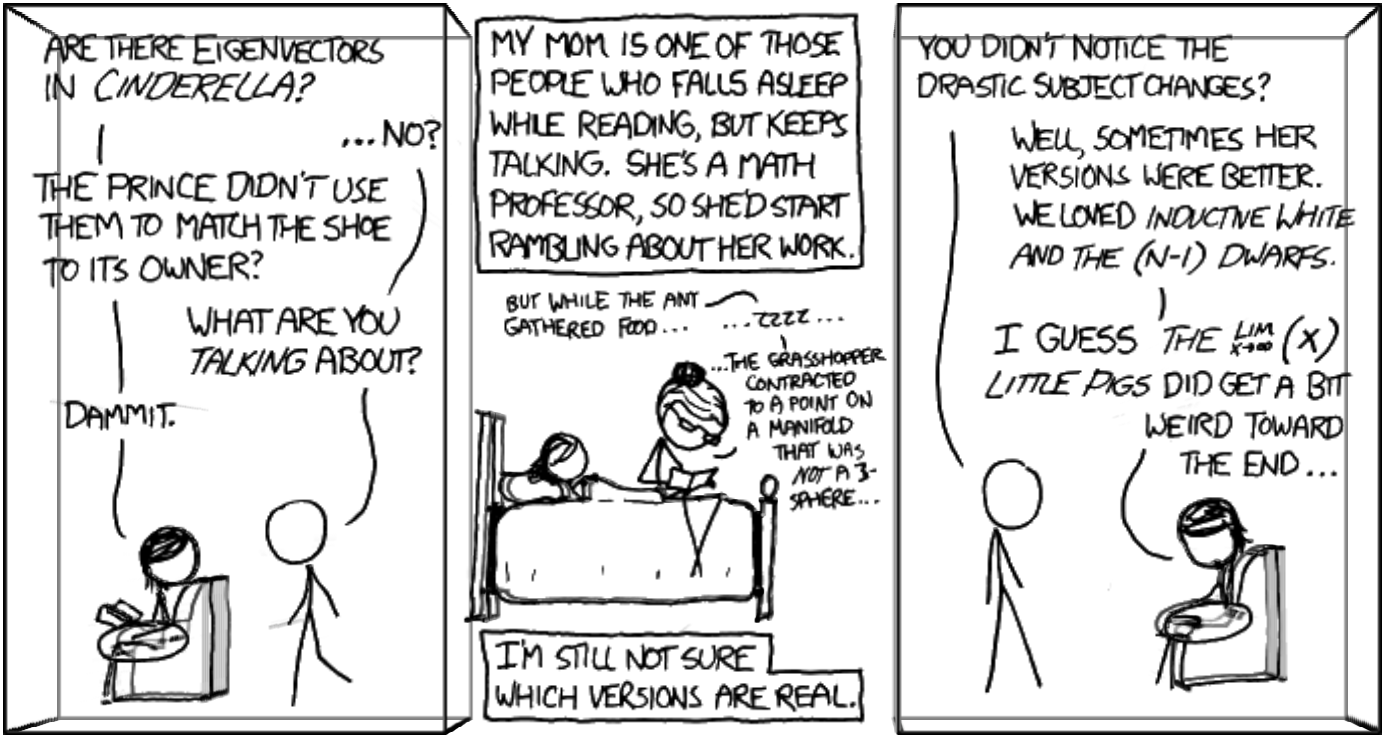
\includegraphics[scale=0.4]{Graphics/eigenvectorxkcd.png}
\end{savequote}
\chapter{Determinants and Eigenvalues}

    \section{Lecture 13: September 21, 2022}

    \subsection{Defining the Determinant}

        Consider the following theorems and definitions.
        \begin{theorem}{\Stop\,\,The Determinant Determines the Area in \(\mathbb{R}^2\)}{areadet}

            Consider \(\vec{x}=[x_1,x_2]\) and \(\vec{y}=[y_1,y_2]\). If we form
            \begin{equation*}
                A=\begin{bmatrix}
                    x_1 & x_2 \\
                    y_1 & y_2 
                \end{bmatrix},
            \end{equation*}
            \begin{equation*}
                |\det A| = ||\vec{x}\times\vec{y}||.
            \end{equation*}
            That is, \(|\det A|\) provides the area of the parallelogram determined by \(\vec{x}\) and \(\vec{y}\).
            
        \end{theorem}
        \begin{theorem}{\Stop\,\,The Determinant Determines the Volume in \(\mathbb{R}^3\)}{voldet}

            Consider \(\vec{x}=[x_1,x_2,x_3]\), \(\vec{y}=[y_1,y_2,y_3]\), and \(\vec{z}=[z_1,z_2,z_3]\).
            If we form
            \begin{equation*}
                A=\begin{bmatrix}
                    x_1 & x_2 & x_3 \\
                    y_1 & y_2 & y_3 \\
                    z_1 & z_2 & z_3
                \end{bmatrix},
            \end{equation*}
            \begin{equation*}
                |\det A| = \vec{x}\cdot(\vec{y}\times\vec{z}).
            \end{equation*}
            That is, \(|\det A|\) provides the volume of the parallelepiped determined by \(\vec{x}\), \(\vec{y}\), and \(\vec{z}\).
            
        \end{theorem}
        \begin{definition}{\Stop\,\,The \((i,j)\) Submatrix}{submatrix}

            Suppose \(A\in\mathcal{M}_{nn}\). The \((i,j)\) submatrix of \(A\) is the \((n-1)\times(n-1)\) matrix obtained by removing the \(i\)th row and the \(j\)th column. We denote this by \(A_{(i,j)}\) 
            
        \end{definition}
        \begin{definition}{\Stop\,\,The \((i,j)\) Minor}{minor}

            Suppose \(A\in\mathcal{M}_{nn}\). The \((i,j)\) minor of \(A\) is the determinant of the \((i,j)\) submatrix of \(A\).
            
        \end{definition}
        \begin{definition}{\Stop\,\,The \((i,j)\) Cofactor}{cofactor}

            Suppose \(A\in\mathcal{M}_{nn}\). The \((i,j)\) cofactor of \(A\) is
            \begin{equation*}
                A_{ij}=(-1)^{i+j}\det (A_{(i,j)}).
            \end{equation*}
            
        \end{definition}
        \begin{definition}{\Stop\,\,The Determinant}{det}
            Suppose \(A\in\mathcal{M}_{nn}\). Then,
            \begin{enumerate}
                \item If \(n=1\), and \(A=\begin{bmatrix} a_{11} \end{bmatrix}\), \(\det A = a_{11}\).
                \item If \(n=2\), and \(A=\begin{bmatrix} a_{11} & a_{12} \\ a_{21} & a_{22} \end{bmatrix}\), \(\det A = a_{11}a_{22}-a_{12}a_{21}\).
                \item If \(n>2\), and \(A=\begin{bmatrix} a_{11} & \cdots & a_{1n} \\ \vdots & \ddots & \vdots \\ a_{n1} & \cdots & a_{nn} \end{bmatrix}\), \(\det A = (a_{11}A_{11}+\cdots+a_{1n}A_{1n})+\cdots+(a_{n1}A_{n1}+\cdots+a_{nn}A_{nn})\).
            \end{enumerate}
        \end{definition}
        \pagebreak
        \vphantom
        \\
        \\
        For fun, consider the following Python 3 implementation of computing the determinant of any \(n\times n\) matrix.
        \lstinputlisting[language=Python]{Graphics/matrixdet.py}
        
        \pagebreak

\section{Lecture 14: September 23, 2022}

    \subsection{Determinants of Upper Triangular Matrices}

        Consider the following theorems.
        \begin{theorem}{\Stop\,\,The Determinant of an Upper Triangular Matrix}{uppertriangulardet}

            If \(A\in\mathcal{M}_{nn}\) is upper triangular, 
            \begin{equation*}
                \det A = a_{11} a_{22} \cdots a_{nn}.
            \end{equation*}
            Recall that \(A\) is upper triangular if and only if all elements below the main diagonal are zero.
            \begin{proof}
                We proceed by induction on \(n\). For \(n=1\), \(A=\begin{bmatrix} a_{11} \end{bmatrix}\), so \(\det A = a_{11}\). Suppose for all \(k\in\mathbb{N}\), and some upper triangular \(A\in\mathcal{M}_{kk}\),
                \begin{equation*}
                    a_{11} a_{22} \cdots a_{kk}.
                \end{equation*}
                Consider 
                \begin{equation*}
                    B=\begin{bmatrix}
                        b_{11} & \cdots & b_{1(k+1)} \\
                        \vdots & \ddots & \vdots \\
                        0 & \cdots & b_{(k+1)(k+1)}
                    \end{bmatrix}.
                \end{equation*}
                Then, we compute \(\det B\) using the last row as our ``first row.''
                \begin{align*}
                    \det B &= (-1)^{1+1}b_{11}\det\begin{bmatrix} b_{22} & b_{23} & \cdots & a_{2(k+1)} \\ 0 & b_{33} & \cdots & b_{3(k+1)} \\ \vdots & \vdots & \vdots & \vdots \\ 0 & 0 & 0 & b_{(k+1)(k+1)} \end{bmatrix} \\
                    &= b_{11}\underbrace{b_{22}\cdots b_{(k+1)(k+1)}}_{\text{By the inductive hypothesis.}}.
                    %\begin{comment}\det B&= 0+\cdots+0+a_{(k+1)(k+1)}(-1)^{(k+1)+(k+1)}\det B_{(k+1),(k+!)} \\ &=a_{(k+1)(k+1)}(-1)^{2(k+1)}\det A.\end{comment}
                \end{align*}
                This is precisely the stipulation of the theorem when \(n=k+1\).
            \end{proof}

        \end{theorem}
        \pagebreak
        \begin{theorem}{\Stop\,\,Determinants and Row Operations}{detrowops}

            Suppose \(A\in\mathcal{M}_{nn}\) and let \(R\) be a row operation. Then,
            \begin{enumerate}
                \item If \(R\) is \(c\langle i\rangle\to\langle i \rangle\) for some \(c\in\mathbb{R}\), 
                \begin{equation*}
                    \det R(A) = c\det A.
                \end{equation*}
                Note that if \(c=0\), \(R\) is not a valid row operation.
                \item If \(R\) is \(c\langle i\rangle+\langle j \rangle\to\langle j \rangle\) for some \(c\in\mathbb{R}\),
                \begin{equation*}
                    \det R(A) = \det A.
                \end{equation*}
                Note that if \(c=0\), \(R\) is not a valid row operation.
                \item If \(R\) is \(\langle i \rangle\leftrightarrow\langle j \rangle\),
                \begin{equation*}
                    \det R(A) = -\det A.
                \end{equation*}
            \end{enumerate}
            \vphantom
            \\
            \\
            Note that if \(\det A\neq 0\) and \(R\) is a row operation, \(\det R(A)\neq 0\).
        \end{theorem}
        \vphantom
        \\
        \\
        We can use Theorem \ref{thm:detrowops} in conjunction with row operations to compute the determinant of a matrix easily. We simply use row operations to create an upper triangular matrix, while keeping track of how the determinant changes. We then apply Theorem \ref{thm:uppertriangulardet}. Consider the following examples.
        \begin{example}{\Difficulty\,\Difficulty\,\,Computing a Determinant by Row Reduction}{compdetrowred}
            
            Compute \(\det\begin{bmatrix} 1 & 1 & 1 \\ 2 & 3 & -2 \\ 4 & 9 & 4 \end{bmatrix}\).
            \\
            \\
            Let 
            \begin{equation*}
                A_0=\begin{bmatrix} 1 & 1 & 1 \\ 2 & 3 & -2 \\ 4 & 9 & 4 \end{bmatrix}.
            \end{equation*}
            Consider the following table.
            \begin{center}
                \begin{tabular}{||c|c|c||}
                    \hline
                    Row Operation & Resultant Matrix & Effect on the Determinant \\
                    \hline
                    \hline
                    \(-2\langle1\rangle+\langle2\rangle\to\langle2\rangle\) & \(A_1=\begin{bmatrix} 1 & 1 & 1 \\ 0 & 1 & -4 \\ 4 & 9 & 4 \end{bmatrix}\) & \(\det A_1=\det A_0\) \\
                    \hline
                    \(-4\langle1\rangle+\langle3\rangle\to\langle3\rangle\) & \(A_2=\begin{bmatrix} 1 & 1 & 1 \\ 0 & 1 & -4 \\ 0 & 5 & 0 \end{bmatrix}\) & \(\det A_2=\det A_1\) \\
                    \hline
                    \(-5\langle2\rangle+\langle3\rangle\to\langle3\rangle\) & \(A_3=\begin{bmatrix} 1 & 1 & 1 \\ 0 & 1 & -4 \\ 0 & 0 & 20 \end{bmatrix}\) & \(\det A_3=\det A_2\) \\
                    \hline
                \end{tabular}
            \end{center}
            \vphantom
            \\
            \\
            Thus, \(\det A_0=20\).

        \end{example}
        \pagebreak
        \begin{example}{\Difficulty\,\Difficulty\,\,Computing a Determinant by Row Reduction}{compdetrowred}
            
            Compute \(\det\begin{bmatrix} 0 & -14 & -8 \\ 1 & 3 & 2 \\ -2 & 0 & 6 \end{bmatrix}\).
            \\
            \\
            Let 
            \begin{equation*}
                A_0=\begin{bmatrix} 0 & -14 & -8 \\ 1 & 3 & 2 \\ -2 & 0 & 6 \end{bmatrix}.
            \end{equation*}
            Consider the following table.
            \begin{center}
                \begin{tabular}{||c|c|c||}
                    \hline
                    Row Operation & Resultant Matrix & Effect on the Determinant \\
                    \hline
                    \hline
                    \(\langle2\rangle\leftrightarrow\langle1\rangle\) & \(A_1=\begin{bmatrix} 1 & 3 & 2 \\ 0 & -14 & -8 \\ -2 & 0 & 6 \end{bmatrix}\) & \(\det A_1=-\det A_0\) \\
                    \hline
                    \(2\langle1\rangle+\langle3\rangle\to\langle3\rangle\) & \(A_2=\begin{bmatrix} 1 & 3 & 2 \\ 0 & -14 & -8 \\ 0 & 6 & 10 \end{bmatrix}\) & \(\det A_2=\det A_1\) \\
                    \hline
                    \(-\frac{1}{14}\langle2\rangle\to\langle2\rangle\) & \(A_3=\begin{bmatrix} 1 & 3 & 2 \\ 0 & 1 & \frac{4}{7} \\ 0 & 6 & 10 \end{bmatrix}\) & \(\det A_3=-\frac{1}{14}\det A_2\) \\
                    \hline
                    \(-6\langle2\rangle+\langle3\rangle\to\langle3\rangle\) & \(A_3=\begin{bmatrix} 1 & 3 & 2 \\ 0 & 1 & \frac{4}{7} \\ 0 & 0 & \frac{46}{7} \end{bmatrix}\) & \(\det A_4=\det A_3\) \\
                    \hline
                \end{tabular}
            \end{center}
            \vphantom
            \\
            \\
            Thus, \(\det A_0=\frac{46}{7}(-14)(-1)=92\).

        \end{example}
        \vphantom
        \\
        \\
        Consider the following theorem.
        \begin{theorem}{\Stop\,\,Inverses and Determinants}{invdet}
            
            Suppose that \(A\in\mathcal{M}_{nn}\). Then, \(A\) is nonsingular if and only if \(\det A \neq 0\).
            \begin{proof}
                If \(A\) is nonsingular, we can row reduce \(A\) to produce \(I_n\). Since \(\det I_n\neq 0\), by Theorem \ref{thm:detrowops}, \(\det A\neq 0\). If \(\det A\neq 0\), we form the system \([A|B]\) and reduce it to \([C|D]\). We know that \(\det C\neq 0\). Because \(C\) is in reduced row echelon form, and square since \(A\) is square, it is upper triangular. That means all main diagonal entries are nonzero, meaning they are all \(1\). Meaning \(C=I_n\). This means we were able to row reduce \(A\) to \(I_n\), so \(A\) is nonsingular.
            \end{proof}
            
        \end{theorem}
        \vphantom
        \\
        \\
        Consider the following table summarizing various results. Statements in each column are equivalent.
        \begin{center}
            \begin{tabular}{||c|c||}
                \hline
                \hline
                \(A\in\mathcal{M}_{nn}\) is Nonsingular & \(A\in\mathcal{M}_{nn}\) is Singular \\
                \hline
                \hline
                \(\rank A = n\) & \(\rank A < n\) \\
                \(\det A \neq 0\) & \(\det A = 0\) \\
                \(A\) is row equivalent to \(I_n\). & \(A\) is not row equivalent to \(I_n\). \\
                \(AX=0\) has only the trivial solution for \(X\). & \(AX=0\) has a nontrivial solution for \(X\). \\
                \(AX=B\) has a unique solution for \(X\), and \(X=A^{-1}B\). & \(AX=B\) does not have a unique solution. \\
                \hline
            \end{tabular}
        \end{center}

\pagebreak

\section{Lecture 15: September 26, 2022}

    \subsection{Further Properties of Determinants}

        \begin{theorem}{\Stop\,\,Properties of Determinants}{detprop}

            Suppose \(A,B\in\mathcal{M}_{nn}\). Then,
            \begin{enumerate}
                \item \(\det (AB) = \det A\det B\).
                \begin{proof}
                    If \(A\) or \(B\) is singular, \(\det A\det B=0\). For now, let \(B\) be singular. We don't make any assumptions about \(A\), for now. Since \(B\) is singular, there exists some \(X\neq0\) such that \(BX=0\). We consider \((AB)X=A(BX)=A(0)=0\). Thus, \(X\) is a nontrivial solution to the homogeneous equation associated with \(AB\). Thus \(AB\) is singular and \(\det (AB) = 0 = \det A\det B\). Now, suppose that \(A\) is singular and \(B\) is nonsingular. There exists a nontrivial solution for \(Y\) in the system \(AY=0\). Since \(B\) is nonsingular, \(B^{-1}\) exists. We define \(X=B^{-1}Y\) where \(X\neq0\). Then \(ABX=AB(B^{-1}Y)=AY=0\). Thus, \(ABX\) and \(X\neq 0\) implies that \(AB\) is singular, so \(\det (AB)=0\). Now, we consider the case where \(A\) and \(B\) are both nonsingular. There exists row operations \(R_1,\ldots,R_k\) such that \(A=R_1(\ldots(R_k(I_n)\ldots))\) and 
                    \begin{align*}
                        \det (AB)&=\det(R_1(\ldots(R_k(I_n)\ldots))B) \\
                        &=c_1\cdots c_k\det (I_nB) \\
                        &=c_1\cdots c_k\det B \\
                        &=c_1\cdots c_k \det I_n\det B \\
                        &=\det(R_1(\ldots(R_k(I_n)\ldots)))\det B \\
                        &=\det A\det B,
                    \end{align*}
                    hence proving the proposition.
                \end{proof}
                \item \(\det (A^T) = \det A\).
                \begin{proof}
                    Suppose that \(A\) is singular, meaning \(\det A=0\). We seek to show that then, \(\det (A^T)=0\). Suppose, for the sake of contradiction, \(\det (A^T)\neq0\), meaning \(A^T\) is nonsingular. Then, \((A^T)^T=A\) is also nonsingular, which contradicts our assumption. Suppose that \(A\) is nonsingular, meaning \(A\) is row equivalent to \(I_n\). That means
                    \begin{equation*}
                        \det A = \det(R_k(\ldots R_2(R_1(I_n))\ldots))=\det((R_k(\ldots R_2(R_1(I_n))\ldots))^T)=\det (A^T),
                    \end{equation*}
                    proving the proposition.
                \end{proof}
                \item \(\underbrace{\det (A^{-1}) = \frac{1}{\det A}}_{\text{Suppose that \(A\) is nonsingular.}}\).
                \begin{proof}
                    We know that \(A\) is nonsingular. We have \(\det I_n=\det(AA^{-1})=\det A\det (A^{-1})=1\). By simple algebra, \(\det (A^{-1})=\frac{1}{\det A}\).
                \end{proof}
            \end{enumerate}
            
        \end{theorem}

    \pagebreak

    \subsection{Eigenvectors, Eigenvalues, and Diagonalization}

        Consider the following definitions and theorems.

        \begin{definition}{\Stop\,\,Similarity}{sim}

            Suppose \(A,B\in\mathcal{M}_{nn}\). The matrix \(B\) is similar to a matrix \(A\) if and only if there exists some nonsingular matrix \(P\) such that
            \begin{equation*}
                B=P^{-1}AP.
            \end{equation*}

        \end{definition}
        \begin{definition}{\Stop\,\,Diagonalizability}{diagonalizability}

            The matrix \(A\in\mathcal{M}_{nn}\) is diagonalizable if and only if a diagonal matrix \(D\) is similar to \(A\). That is, \(A\) is diagonalizable if and only if, for nonsingular matrix \(P\),
            \begin{equation*}
                D=P^{-1}AP.
            \end{equation*}
            
        \end{definition}
        \begin{definition}{\Stop\,\,Eigenvalues and Eigenvectors}{eigenvaluesandvectors}

            For \(A\in\mathcal{M}_{nn}\), \(\lambda\in\mathbb{R}\) is an eigenvalue of \(A\) if and only if there exists \(X\neq0\) such that
            \begin{equation*}
                AX=\lambda X.
            \end{equation*}
            If \(\lambda\) is an eigenvalue of \(A\), \(X\) is an eigenvector of \(A\) with eigenvalue \(\lambda\).

        \end{definition}

        \pagebreak

\section{Lecture 16: September 28, 2022}

    \subsection{The Process of Diagonalization: Part I}

        Consider the following definition.
        \begin{definition}{\Stop\,\,Eigenspace}{eigenspace}

            Given \(A\in\mathcal{M}_{nn}\), the eigenspace of a given eigenvalue \(\lambda\) is
            \begin{equation*}
                E_\lambda=\{X:AX=\lambda X\}\cup\{\vec{0}\}
            \end{equation*}
            Note that ``\(\cup \{\vec{0}\}\)'' is somewhat redundant, as it will always satisfy the equation. However, the zero vector is never an eigenvector.

        \end{definition}
        \vphantom
        \\
        \\
        Our goal is to find all the eigenvalues and eigenspaces of \(A\). Consider the following theorem.
        \begin{theorem}{\Stop\,\,Finding Eigenvectors and Eigenvalues}{findeigenvs}
    
            Consider a matrix \(A\in\mathcal{M}_{nn}\). By definition, \(X\) is an eigenvector of \(A\) with eigenvalue \(\lambda\in\mathbb{R}\) when
            \begin{equation*}
                AX=\lambda X=\lambda I_nX.
            \end{equation*}
            That is, when
            \begin{equation*}
                (A-\lambda I_n)X=\vec{0}.
            \end{equation*}
            The above equation has a nontrivial solution for \(X\) if and only if \((A-\lambda I_n)\) is singular, that is, when
            \begin{equation*}
                \det(A-\lambda I_n)=0.
            \end{equation*}
            Therefore, the scalar \(\lambda\) is an eigenvalue of \(A\) if and only if \(\lambda\) satisfies the above equation.
        \end{theorem}
        \pagebreak
        \vphantom
        \\
        \\
        Note that, for now, we will only consider real eigenvalues; however, complex eigenvalues are incredibly useful and have numerous applications. Consider the following example.
        \begin{example}{\Difficulty\,\,Eigenspaces of A Diagonal Matrix}{eigdiag}

            Consider \(A=\begin{bmatrix} 5 & 0 & 0 \\ 0 & 7 & 0 \\ 0 & 0 & 7 \end{bmatrix}\). Find the eigenvalues and eigenspaces of \(A\).
            \\
            \\
            We see that the eigenvalues are \(\lambda_1=5\) and \(\lambda_2=7\). The eigenspaces are
            \begin{equation*}
                E_{\lambda_1}=\left\{c\begin{bmatrix} 1 \\ 0 \\ 0 \end{bmatrix}:c\in\mathbb{R}\right\}
            \end{equation*}
            and
            \begin{equation*}
                E_{\lambda_2}=\left\{c_1\begin{bmatrix} 0 \\ 1 \\ 0 \end{bmatrix}+c_2\begin{bmatrix} 0 \\ 0 \\ 1 \end{bmatrix}:c_1,c_2\in\mathbb{R}\right\}.
            \end{equation*}

        \end{example}
        \pagebreak
        \vphantom
        \\
        \\
        We note that for a diagonal matrix, we can simply read off the eigenvalues and eigenspaces. Generally though, we use Theorem \ref{thm:findeigenvs}, as seen in the following example.
        \begin{example}{\Difficulty\,\Difficulty\,\,Eigenspaces of a \(2\times 2\) Matrix}{eig22}
            
            Consider \(A=\begin{bmatrix} 7 & 1 \\ -3 & 3 \end{bmatrix}\). Find the eigenvalues and eigenspaces of \(A\).
            \\
            \\
            To find the eigenvalues, we consider
            \begin{align*}
                \det(A-\lambda I_2)&=\det \begin{bmatrix} 7-\lambda & 1 \\ -3 & 3-\lambda \end{bmatrix} \\
                &=(7-\lambda)(3-\lambda)+3 \\
                &=21-10\lambda+\lambda^2+3 \\
                &=\lambda^2-10\lambda+24 \\
                &=0.
            \end{align*}
            By factoring, we have \((\lambda-6)(\lambda-4)=0\), meaning \(\lambda_1=4\) and \(\lambda_2=6\). Now, we seek to find the eigenspace. We substitute in \(\lambda_1\) and \(\lambda 2\) into \((A-\lambda I_2)=0\) and solve for \(\lambda\). For \(\lambda_1\), we have
            \begin{align*}
                \begin{bmatrix} 0 \\ 0 \end{bmatrix}&=\begin{bmatrix} 7-4 & 1 \\ -3 & 3-4 \end{bmatrix} \\
                &=\begin{bmatrix} 3 & 1 \\ -3 & -1 \end{bmatrix}.
            \end{align*}
            By row reduction, we have
            \begin{equation*}
                \begin{bmatrix} 0 \\ 0 \end{bmatrix}=\begin{bmatrix} 1 & \frac{1}{3} \\ 0 & 0 \end{bmatrix}
            \end{equation*}
            and
            \begin{equation*}
                E_{\lambda_1}=\left\{\begin{bmatrix} -\frac{1}{3}c \\ c \end{bmatrix}: c\in\mathbb{R}\right\}.
            \end{equation*}
            By a similar process, we have
            \begin{equation*}
                E_{\lambda_2}=\left\{\begin{bmatrix} -c \\ c \end{bmatrix}: c\in\mathbb{R}\right\}.
            \end{equation*}

        \end{example}
        \pagebreak
        \vphantom
        \\
        \\
        Now, we revisit Definition \ref{def:sim}. How do we find \(D\) and \(P\)? We take \(D\) to be the diagonal matrix with all nonzero elements being the eigenvalues of \(A\). Then, we take \(P\) to be the matrix with each column being the eigenvector associated with the eigenvalue in the corresponding column of \(D\). Finally, we check that \(P^{-1}\) exists. Why does this work? In the general \(2\times 2\) case, we have
        \begin{equation*}
            D=\begin{bmatrix}
                \lambda_1 & 0 \\ 0 & \lambda_2
            \end{bmatrix}
        \end{equation*}
        and \(P=\begin{bmatrix} \vec{v}_1 & \vec{v}_2 \end{bmatrix}\) where \(\vec{v}_1\) and \(\vec{v}_2\) are eigenvectors of \(A\), associated with eigenvalues \(\lambda_1\) and \(\lambda_2\), respectively. We have checked that \(P^{-1}\) exists and has the form \(P^{-1}=\begin{bmatrix} \vec{w}_1 \\ \vec{w}_2 \end{bmatrix}\). Then, 
        \begin{equation*}
            P^{-1}P=\begin{bmatrix} \vec{w}_1\cdot\vec{v}_1 & \vec{w}_1\cdot\vec{v}_2 \\ \vec{w}_2\cdot\vec{v}_1 & \vec{w}_2\cdot\vec{v}_2 \end{bmatrix}=I_2.
        \end{equation*}
        Then, we have
        \begin{align*}
            P^{-1}AP&=P^{-1}(AP) \\
            &=P^{-1}\begin{bmatrix} A\vec{v}_1 & A\vec{v}_2 \end{bmatrix} \\
            &=P^{-1}\begin{bmatrix} \lambda_1\vec{v}_1 & \lambda_2\vec{v}_2 \end{bmatrix} \\
            &=\begin{bmatrix} \vec{w}_1 \\ \vec{w}_2 \end{bmatrix}\begin{bmatrix} \lambda_1\vec{v}_1 & \lambda_2\vec{v}_2 \end{bmatrix} \\
            &=\begin{bmatrix} \lambda_1\vec{w}_1\cdot\vec{v}_1 & \lambda_2\vec{w}_1\cdot\vec{v}_2 \\ \lambda_1\vec{w}_2\cdot\vec{v}_1 & \lambda_2\vec{w}_2\cdot\vec{v}_2 \end{bmatrix} \\
            &=\begin{bmatrix} \lambda_1 & 0 \\ 0 & \lambda_2 \end{bmatrix} \\
            &=D.
        \end{align*}

\pagebreak

\section{Lecture 17: September 30, 2022}

    \subsection{The Process of Diagonalization: Part II}

        We summarize the process of diagonalization in a more general sense.
        \begin{theorem}{\Stop\,\,The Process of Diagonalization}{diagonalization}
            Let \(A\in\mathcal{M}_{nn}\), consider the following steps.
            \begin{enumerate}
                \item Find the solutions of \(\det(A-\lambda I_n)=0\). The solutions \(\lambda_1,\ldots,\lambda_k\) are the eigenvalues of \(A\).
                \item For each eigenvalue \(\lambda_m\), solve the system \([A-\lambda_mI_n|0]\) by row reduction.
                \item If there are less than \(n\) fundamental eigenvectors, \(A\) cannot be diagonalized.
                \item Form \(P=\begin{bmatrix} \vec{v}_1 & \cdots & \vec{v}_n \end{bmatrix}\). Note that \(P\) is nonsingular.
                \item Verify that \(D=P^{-1}AP\) is a diagonal matrix where each entry \(d_{ii}\) is the eigenvalue for the fundamental eigenvector forming the \(i\)th column of \(P\).
            \end{enumerate}
        \end{theorem}
        \pagebreak
        \vphantom
        \\
        \\
        Consider the following examples.
        \begin{example}{\Difficulty\,\Difficulty\,\,Diagonalization 1}{diag1}

            Given
            \begin{equation*}
                A=\begin{bmatrix}
                    9 & 5 \\ 
                    -25 & -21
                \end{bmatrix},
            \end{equation*}
            construct the diagonal matrix \(D\) and form the nonsingular matrix \(P\) such that
            \begin{equation*}
                D=P^{-1}AP.
            \end{equation*}
            To find the eigenvalues, we have
            \begin{align*}
                0&=\det\begin{bmatrix}
                    9-\lambda & 5 \\
                    -25 & -21-\lambda
                \end{bmatrix} \\
                &=(9-\lambda)(-21-\lambda)+125 \\
                &=(\lambda+16)(\lambda-4).
            \end{align*}
            Therefore, our eigenvalues are \(\lambda_1=-16\) and \(\lambda_2=4\). To find the associated eigenvectors, for \(\lambda_1\), we have
            \begin{equation*}
                \begin{bmatrix}
                    25 & 5 & | & 0 \\
                    -25 & -5 & | & 0
                \end{bmatrix},
            \end{equation*}
            which, by \(\langle1\rangle\to\langle2\rangle\to\langle2\rangle\), becomes
            \begin{equation*}
                \begin{bmatrix}
                    25 & 5 & | & 0 \\
                    0 & 0 & | & 0
                \end{bmatrix}.
            \end{equation*}
            We have the eigenspace \(E_{-16}=\left\{c\begin{bmatrix} -1 \\ 5 \end{bmatrix}:c\in\mathbb{R}\right\}\). For \(\lambda_2\), we have
            \begin{equation*}
                \begin{bmatrix}
                    5 & 5 & | & 0 \\
                    -25 & -25 & | & 0
                \end{bmatrix}
            \end{equation*} 
            which can be row reduced to
            \begin{equation*}
                \begin{bmatrix}
                    -25 & -25 & | & 0 \\
                    0 & 0 & | & 0 \\
                \end{bmatrix}.
            \end{equation*} 
            This produces the eigenspace \(E_4=\left\{c\begin{bmatrix} -1 \\ 1 \end{bmatrix}:c\in\mathbb{R}\right\}\). We form 
            \begin{equation*}
                D=\begin{bmatrix} -16 & 0 \\ 0 & 4 \end{bmatrix},\quad P=\begin{bmatrix} -1 & -1 \\ 5 & 1 \end{bmatrix},\quad P^{-1}=\begin{bmatrix} \frac{1}{4} & \frac{1}{4} \\ -\frac{5}{4} & -\frac{1}{4} \end{bmatrix}.
            \end{equation*}
            To check our work, we have
            \begin{align*}
                P^{-1}AP&=\begin{bmatrix} \frac{1}{4} & \frac{1}{4} \\ -\frac{5}{4} & -\frac{1}{4} \end{bmatrix} \begin{bmatrix} 9 & 5 \\ -25 & 21 \end{bmatrix} \begin{bmatrix} -1 & -1 \\ 5 & 1 \end{bmatrix} \\
                &=\begin{bmatrix} -16 & 0 \\ 0 & 4 \end{bmatrix} \\
                &=D,
            \end{align*}
            thus verifying our answer.
        \end{example}
        \begin{example}{\Difficulty\,\Difficulty\,\,Diagonalization 2}{diag2}

            Given
            \begin{equation*}
                A=\begin{bmatrix}
                    0 & -6 & 0 \\
                    3 & 9 & 0 \\
                    0 & 0 & 6
                \end{bmatrix},
            \end{equation*}
            construct the diagonal matrix \(D\) and form the nonsingular matrix \(P\) such that
            \begin{equation*}
                D=P^{-1}AP.
            \end{equation*}
            To find the eigenvalues, we have
            \begin{align*}
                0&=\det\begin{bmatrix}
                    -\lambda & -6 & 0 \\
                    3 & 9-\lambda & 0 \\
                    0 & 0 & 6-\lambda
                \end{bmatrix} \\
                &=-\lambda((9-\lambda)(6-\lambda))+6(3(6-\lambda)) \\
                &=-(\lambda-3)(\lambda-6)^2.
            \end{align*}
            Therefore, our eigenvalues are \(\lambda_1=3\) and \(\lambda_2=6\). For \(\lambda_1\), we have the linear system
            \begin{equation*}
                \begin{bmatrix}
                    -3 & -6 & 0 & | & 0 \\
                    0 & 0 & 0 & | & 0 \\
                    0 & 0 & 3 & | & 0 \\
                \end{bmatrix}
            \end{equation*}
            which can be row reduced to
            \begin{equation*}
                \begin{bmatrix}
                    1 & 2 & 0 & | & 0 \\
                    0 & 0 & 1 & | & 0 \\
                    0 & 0 & 0 & | & 0 
                \end{bmatrix}.
            \end{equation*}
            This gives us \(E_3=\left\{c\begin{bmatrix} -2 \\ 1 \\ 0 \end{bmatrix}:c\in\mathbb{R}\right\}\). For \(\lambda_2\), we have
            \begin{equation*}
                \begin{bmatrix}
                    -6 & -6 & 0 & | & 0 \\
                    3 & 3 & 0 & | & 0 \\
                    0 & 0 & 0 & | & 0
                \end{bmatrix},
            \end{equation*}
            which can be row reduced to
            \begin{equation*}
                \begin{bmatrix}
                    1 & 1 & 0 & | & 0 \\
                    0 & 0 & 0 & | & 0 \\
                    0 & 0 & 0 & | & 0
                \end{bmatrix},
            \end{equation*}
            giving
            \begin{align*}
                E_6&=\left\{\begin{bmatrix} -c_1 \\ c_1 \\ c_2 \end{bmatrix}:c_1,c_2\in\mathbb{R}\right\} \\ 
                &=\left\{c_1\begin{bmatrix} -1 \\ 1 \\ 0 \end{bmatrix}+c_2\begin{bmatrix} 0 \\ 0 \\ 1 \end{bmatrix}:c_1,c_2\in\mathbb{R}\right\}
            \end{align*}   
            We can then form
            \begin{equation*}
                D=\begin{bmatrix} 3 & 0 & 0 \\ 0 & 6 & 0 \\ 0 & 0 & 6 \end{bmatrix},\quad P=\begin{bmatrix} -2 & -1 & 0 \\ 1 & 1 & 0 \\ 0 & 0 & 1 \end{bmatrix},\quad P^{-1}=\begin{bmatrix} -1 & -1 & 0 \\ 1 & 2 & 0 \\ 0 & 0 & 1 \end{bmatrix}.
            \end{equation*}    
        \end{example}

        \begin{comment}
            \begin{example}{\Difficulty\,\Difficulty\,\,Diagonalizing a Matrix 1}{diagmat1}

            Construct the diagonal matrix \(D\), given
            \begin{equation*}
                A=\begin{bmatrix}
                    -4 & 8 & -12 \\
                    6 & -6 & 12 \\
                    6 & -8 & 14
                \end{bmatrix}.
            \end{equation*}
            We construct the equation
            \begin{align*}
                0&=\det \begin{bmatrix}
                    -4-\lambda & 8 & -12 \\
                    6 & -6-\lambda & 12 \\
                    6 & -8 & 14-\lambda
                \end{bmatrix}. \\
                &=(-4-\lambda)((-6-\lambda)(14-\lambda)+96)-8(6(14-\lambda)-72)-12(-48-6(-6-\lambda)) \\
                &=-x(x-2)^2.
            \end{align*}
            Thus, the eigenvalues are \(\lambda_1=0\) and \(\lambda_2=2\). For \(\lambda_1\), we have the system
            \begin{equation*}
                \begin{bmatrix}
                    -4 & 8 & -12 & | & 0 \\
                    6 & -6 & 12 & | & 0 \\
                    6 & -8 & 14 & | & 0
                \end{bmatrix}.
            \end{equation*}
            By row reduction, we have
            \begin{equation*}
                \begin{bmatrix}
                    1 & 0 & 1 & | & 0 \\
                    0 & 1 & -1 & | & 0 \\
                    0 & 0 & 0 & | & 0.
                \end{bmatrix}.
            \end{equation*}
            Now, \(E_{\lambda_1}=\left\{\begin{bmatrix} -c \\ c \\ c \end{bmatrix}:c\in\mathbb{R}\right\}\). For \(\lambda_2\), we have 
            \begin{equation*}
                \begin{bmatrix}
                    -6 & 8 & -12 & | & 0 \\
                    6 & -8 & 12 & | & 0 \\
                    6 & -8 & 12 & | & 0
                \end{bmatrix},
            \end{equation*}
            which can be reduced to
            \begin{equation*}
                \begin{bmatrix}
                    1 & -\frac{4}{3} & 2 & | & 0 \\
                    0 & 0 & 0 & | & 0 \\
                    0 & 0 & 0 & | & 0
                \end{bmatrix}.
            \end{equation*}
            After removing fractions, we have
            \begin{equation*}
                \begin{bmatrix}
                    3 & -4 & 6 & | & 0 \\
                    0 & 0 & 0 & | & 0 \\
                    0 & 0 & 0 & | & 0
                \end{bmatrix}.
            \end{equation*}
        \end{example}
    \end{comment}

\pagebreak

\section{Lecture 18: October 3, 2022}

    \subsection{The Process of Diagonalization: Part III}

        We start with a question; what can go wrong in the diagonalization process? We will trace each step of Theorem \ref{thm:diagonalization}. 
        \begin{center}
            \begin{tabular}{||c|c||}
                \hline
                \hline
                What Could go Wrong? & Example \\
                \hline
                \hline
                There exist complex roots to \(\det(A-\lambda I_n)=0\). & \(A=\begin{bmatrix} 0 & -1 \\ 1 & 0 \end{bmatrix}\) \\
                \hline
                There are less than \(n\) fundamental eigenvectors. & \(A=\begin{bmatrix} 7 & 1 \\ 0 & 7 \end{bmatrix}\) \\
                \hline
            \end{tabular}
        \end{center}
        \vphantom
        \\
        \\
        We remark that if there exist complex roots, we can resolve it by considering complex eigenvalues in the diagonalization process, as seen in Example \ref{exa:compdiag}; however, we cannot resolve the issue of having less than \(n\) fundamental eigenvectors. Naturally, the question of what constitutes a fundamental eigenvector is brought up. Consider the following definitions and theorems.
        \begin{definition}{\Stop\,\,Linear Independence}{linindep}
            
            Suppose \(\vec{v}_1,\ldots,\vec{v}_k\) are vectors in \(\mathbb{R}^n\). The set \(\{\vec{v}_1,\ldots,\vec{v}_k\}\) is linearly independent if and only if all scalars \(c_1,\ldots,c_k\) that form
            \begin{equation*}
                c_1\vec{v}_1+\cdots+c_k\vec{v}_k=\vec{0}
            \end{equation*}
            are zero.

        \end{definition}
        \begin{theorem}{\Stop\,\,Diagonalizability}{diagonalizability}

            The matrix \(A\in\mathcal{M}_{nn}\) is diagonalizable if and only if there exists a set \(S=\{\vec{v}_1,\ldots,\vec{v}_n\}\) such that
            \begin{enumerate}
                \item Each \(\vec{v}_i\) is an eigenvector of \(A\).
                \item The set \(S\) is linearly independent.
            \end{enumerate}

        \end{theorem}
        \vphantom
        \\
        \\
        The statement ``There are less than \(n\) fundamental eigenvectors'' means that the set \(S=\{\vec{v}_1,\ldots,\vec{v}_n\}\) is not linearly independent, or equivalently, linearly dependent. To conclude if we will have a sufficient number of fundamental eigenvectors, we solve the linear homogeneous system
        \begin{equation*}
            \begin{bmatrix}
                \vec{v}_1 & \cdots & \vec{v}_n | \vec{0}
            \end{bmatrix}
        \end{equation*}
        for \(c_1,\ldots,c_n\). Consider the following theorem.
        \begin{theorem}{\Stop\,\,Diagonalizability and Rank}{diagandrank}
            
            Suppose \(A\in\mathcal{M}_{nn}\) with \(\det(A-\lambda I_n)=(x-\lambda_1)^{n_1}\cdots(x-\lambda_\ell)^{n_\ell}\) for 
            \(\lambda_1,\ldots,\lambda_\ell\in\mathbb{R}\). Then, there exists P=\(\begin{bmatrix} \vec{v}_1 & \cdots & \vec{v}_n \end{bmatrix}\) where \(P\) is nonsingular and each \(\vec{v}_i\) is an eigenvector if and only if, for each \(\lambda_i\),
            \begin{equation*}
                \rank(A-\lambda_iI_n)=n-n_i.
            \end{equation*}
            
        \end{theorem}
        \pagebreak
        \vphantom
        \\
        \\
        Consider the following example.
        \begin{example}{\Difficulty\,\Difficulty\,\,Is \(A\) Diagonalizable?}{isitdiag}
            
            Suppose \(A\in\mathcal{M}_{nn}\) and \(\det(A-\lambda I_n)=(x-\lambda_1)(x-\lambda_2)\cdots(x-\lambda_n)\), where \(\lambda_1,\ldots,\lambda_n\in\mathbb{R}\) and \(\lambda_1<\lambda_2\cdots<\lambda_n\). Is \(A\) diagonalizable?
            \\
            \\
            The matrix \(A\) is diagonalizable and
            \begin{equation*}
                D=\begin{bmatrix} 
                    \lambda_1 & \cdots & 0 \\
                    \vdots & \ddots & \vdots \\
                    0 & \cdots & \lambda_n
                \end{bmatrix}.
            \end{equation*}
            The matrix is diagonalizable if all roots \(\lambda_1,\ldots,\lambda_n\) are distinct.

        \end{example}
        \begin{example}{\Difficulty\,\Difficulty\,\,A Non-Diagonalizable Matrix}{nondiagmat}

            Given
            \begin{equation*}
                A=\begin{bmatrix}
                    7 & 1 & -1 \\
                    -11 & -3 & 2 \\
                    18 & 2 & -4
                \end{bmatrix},
            \end{equation*}
            construct the diagonal matrix \(D\) and form the nonsingular matrix \(P\) such that
            \begin{equation*}
                D=P^{-1}AP.
            \end{equation*}
            We will skip over the determinant calculation and will, instead, assert that the characteristic polynomial is \((\lambda+2)^2(\lambda-4)\), meaning the eigenvalues are \(\lambda_1=-2\) and \(\lambda_2=4\). The first eigenvalue, \(\lambda_1\), gives the linear system
            \begin{equation*}
                \begin{bmatrix}
                    9 & 1 & -1 & | & 0 \\
                    -11 & -1 & 2 & | & 0 \\
                    18 & 2 & -2 & | & 0
                \end{bmatrix}
            \end{equation*}
            which reduces to
            \begin{equation*}
                \begin{bmatrix}
                    1 & 0 & -\frac{1}{2} & | & 0 \\
                    0 & 1 & \frac{7}{2} & | & 0 \\
                    0 & 0 & 0 & | & 0
                \end{bmatrix},
            \end{equation*}
            giving us the eigenspace \(E_{-2}=\left\{c\begin{bmatrix} 1 \\ -7 \\ 2 \end{bmatrix}:c\in\mathbb{R}\right\}\). Notice that for \(\lambda_1\),
            \begin{equation*}
                \rank(A-\lambda_1I_3)=2\neq3-2=1.
            \end{equation*}
            Therefore, \(A\) cannot be diagonalized; we need not find the eigenspace of \(\lambda_2\), but for the sake of a curious student, we have \(E_4=\left\{c\begin{bmatrix} 1 \\ -1 \\ 2 \end{bmatrix}:c\in\mathbb{R}\right\}\).

        \end{example}
    
    \subsection{Using Diagonalization to Raise Matrices to Powers}

        One useful application of the diagonalization process is raising matrices to powers. Consider the following theorem.
        \begin{theorem}{\Stop\,\,Raising Matrices to Powers}{raisematpow}

            Given a diagonalizable matrix \(A\),
            \begin{equation*}
                A^k=PD^kP^{-1}.
            \end{equation*}
            \begin{proof}
                We proceed by induction. For \(k=2\),
                \begin{equation*}
                    A^2=AA=(PDP^{-1})(PDP^{-1})=PD(P^{-1}P)DP^{-1}=PDI_nDP^{-1}=PD^2P^{-1}.
                \end{equation*}
                Suppose that for all \(m\in\mathbb{N}\), \(A^m=PD^mP^{-1}\). Then,
                \begin{equation*}
                    A^{m+1}=A^mA=PD^mP^{-1}(PDP^{-1})=PD^m(P^{-1}P)DP^{-1}=PD^mI_nDP^{-1}=PD^{m+1}P^{-1},
                \end{equation*}
                proving the theorem.
            \end{proof}
            
        \end{theorem} 

\pagebreak

\section{Lecture 19: October 5, 2022}

    \begin{comment}
        \subsection{}

        Consider \(\vec{v}=[a_1,\ldots,a_n]\). We then form
        \begin{equation*}
            A=\begin{bmatrix}
                a_1 & a_2 & \cdots & a_n \\
                a_1 & a_2 & \cdots & a_n \\
                \vdots & \vdots & \ddots & \vdots \\
                a_1 & a_2 & \cdots & a_n
            \end{bmatrix}.
        \end{equation*}
        We seek to find the eigenvalues. Because \(A\) is singular, \(0\) is an eigenvalue. We also see that \(a_1+\cdots+a_n\) is an eigenvalue with eigenvector \([1,\cdots,1]\).

    \end{comment}

    \subsection{Complex Numbers}

        Consider the following definition.
        \begin{definition}{\Stop\,\,The Complex Numbers}{compnum}

            The set of complex numbers, \(\mathbb{C}\), is given by
            \begin{equation*}
                \mathbb{C}=\{a+bi:a,b\in\mathbb{R},i^2=-1\}.
            \end{equation*}
            
        \end{definition}
        \begin{definition}{\Stop\,\,The Set \(\mathbb{C}^n\)}{compvcspace}

            We define \(\mathbb{C}^n\) as
            \begin{equation*}
                \mathbb{C}^n=\{[z_1,\ldots,z_n]:z_i=\mathbb{C}\}.
            \end{equation*}
            
        \end{definition}
        \vphantom
        \\
        \\
        As a set, \(\mathbb{C}\) can be visualized as \(\mathbb{R}^2\). Consider the following definitions and properties.
        \begin{definition}{\Stop\,\,Definitions of Operations With Complex Numbers}{depcompops}
            
            Let \(a,b,c,d\in\mathbb{R}\). Then, the following operations are defined as follows.
            \begin{enumerate}
                \item \((a+bi)+(c+di):=(a+c)+(b+d)i\).
                \item \(\Re (a+bi):=a,\quad \Im (a+bi):=b\).
                \item \(z=a+bi\in\mathbb{C}\implies||z||:=\sqrt{a^2+b^2}\).
                \item \((a+bi)(c+di):=ac+adi+bci+bdi^2=(ac-bd)+(ad+bc)i\).
                \item \(z=a+bi\in\mathbb{C}\implies\bar{z}:=a-bi\).
            \end{enumerate}

        \end{definition}
        \begin{theorem}{\Stop\,\,Properties of Complex Numbers}{propcomp}
            
            Let \(a,b,c,d\in\mathbb{R}\). Then,
            \begin{enumerate}
                \item \(z\bar{z}=(a+bi)(a-bi)=a^2+b^2=||z||^2\).
                \item \(z\in\mathbb{C}\backslash \{0\}\implies\frac{1}{z}=\frac{a}{a^2+b^2}-\left(\frac{b}{a^2+b^2}\right)\in\mathbb{C}\)
            \end{enumerate}

        \end{theorem}
        \begin{theorem}{\Stop\,\,The Fundamental Theorem of Algebra}{fundthmalg}
            
            If \(p(z)=a_nz^n+\cdots+a_0z^0\) is an \(n\)th degree polynomial with coefficients \(a_0,\ldots,a_n\in\mathbb{C}\), \(p(z)\) has \(n\) complex roots. Note that some roots may be repeated.

        \end{theorem}
        \pagebreak
        \vphantom
        \\
        \\
        We now consider vectors in \(\mathbb{C}^n\) and define their operations.
        \begin{definition}{\Stop\,\,Vector Addition in \(\mathbb{C}^n\)}{compvcadd}

            Let \(\vec{v}=[v_1,\ldots,v_n]\in\mathbb{C}^n\) and \(\vec{w}=[w_1,\ldots,w_n]\in\mathbb{C}^n\). Then,
            \begin{equation*}
                \vec{v}+\vec{w}=[v_1+w_1,\ldots,v_n+w_n].
            \end{equation*}

        \end{definition}
        \begin{definition}{\Stop\,\,Scalar Multiplication in \(\mathbb{C}^n\)}{compscalmult}

            Let \(\vec{v}=[v_1,\ldots,v_n]\in\mathbb{C}^n\) and \(c\in\mathbb{C}\). Then,
            \begin{equation*}
                c\vec{v}=[cv_1,\ldots,cv_n].
            \end{equation*}

        \end{definition}
        \begin{definition}{\Stop\,\,The Dot Product in \(\mathbb{C}^n\)}{compdotprod}

            Let \(\vec{v}=[v_1,\ldots,v_n]\in\mathbb{C}^n\) and \(\vec{w}=[w_1,\ldots,w_n]\in\mathbb{C}^n\). Then,
            \begin{equation*}
                \vec{v}\cdot\vec{w}=v_1\bar{w_1}+\cdots+v_n\bar{w_n}.
            \end{equation*}

        \end{definition}
        \begin{definition}{\Stop\,\,The Magnitude in \(\mathbb{C}^n\)}{compmagn}

            Let \(\vec{v}=[v_1,\ldots,v_n]\in\mathbb{C}^n\). Then,
            \begin{equation*}
                ||\vec{v}||=\sqrt{\vec{v}\cdot\vec{v}}.
            \end{equation*}

        \end{definition}
        \vphantom
        \\
        \\
        Definition \ref{def:compdotprod} provides a good question: do we consider complex conjugates when performing matrix multiplication with matrices of the sort \(\mathcal{M}_{mn}^\mathbb{C}\)? We do not.
        \begin{definition}{\Stop\,\,The Adjoint}{adjoint}

            Given \(A\in\mathcal{M}_{mn}^\mathbb{C}\), 
            \begin{equation*}
                A=\begin{bmatrix}
                    z_{11} & \cdots & z_{1n} \\
                    \vdots & \ddots & \vdots \\
                    z_{m1} & \cdots & z_{mn}
                \end{bmatrix}
                \implies 
                A^*=\begin{bmatrix}
                    \bar{z_{11}} & \cdots & \bar{z_{m1}} \\
                    \vdots & \ddots & \vdots \\
                    \bar{z_{1n}} & \cdots & \bar{z_{mn}}
                \end{bmatrix}
            \end{equation*}

        \end{definition}
        \vphantom
        \\
        \\
        We will now provide a theorem motivating the transpose operation and apply it to our definition of the adjoint.
        \begin{theorem}{\Stop\,\,The Transpose and The Dot Product}{transposedot}
            If \(\vec{v},\vec{w}\in\mathbb{R}^n\), and \(A\in\mathcal{M}_{nn}^\mathbb{R}\), 
            \begin{equation*}
                (A\vec{v})\cdot\vec{w}=\vec{v}\cdot(A^T\vec{w})
            \end{equation*}
        \end{theorem}
        \begin{theorem}{\Stop\,\,The Adjoint and The Dot Product}{transposedot}
            If \(\vec{v},\vec{w}\in\mathbb{C}^n\), and \(A\in\mathcal{M}_{nn}^\mathbb{C}\), 
            \begin{equation*}
                (A\vec{v})\cdot\vec{w}=\vec{v}\cdot(A^*\vec{w})
            \end{equation*}
        \end{theorem}
        \vphantom
        \\
        \\
        The analog of symmetric and skew-symmetric matrices is the notion of hermitian and skew-hermitian matrices. Consider the following definition. It may also be useful to recall Definition \ref{def:symmetricmatrices}.
        \begin{definition}{\Stop\,\,Hermitian and Skew-Hermitian Matrices}{hermitskewhermit}

            Suppose \(A\in\mathcal{M}_{nn}^\mathbb{C}\). Then,
            \begin{enumerate}
                \item \(A\) is hermitian if and only if \(A=A^*\).
                \item \(A\) is skew-hermitian if and only if \(A=-A^*\).
                \item \(A\) is normal if and only if \(AA^*=A^*A\).
            \end{enumerate}
            
        \end{definition}

\pagebreak

\section{Lecture 20: October 7, 2022}

    \subsection{Diagonalization Using Complex Eigenvalues}

        We now consider the diagonalization process for matrices of the sort \(A\in\mathcal{M}_{nn}^\mathbb{C}\). Consider the following motivating example.
        \begin{example}{\Difficulty\,\Difficulty\,\,Diagonalization With Complex Eigenvalues}{compdiag}

            Diagonalize the matrix
            \begin{equation*}
                A=\begin{bmatrix}
                    0 & 1 \\
                     -1 & 0
                \end{bmatrix}.
            \end{equation*}
            The roots of the characteristic polynomial, \(\det(A-\lambda I_2)\) are \(\lambda_1=i\) and \(\lambda_2=-i\). For \(\lambda_1\), we have
            \begin{equation*}
                \begin{bmatrix}
                    i & -1 & | & 0 \\
                    1 & i & | & 0
                \end{bmatrix}.
            \end{equation*}
            We perform \(\langle1\rangle\leftrightarrow\langle2\rangle\) to obtain
            \begin{equation*}
                \begin{bmatrix}
                    1 & i & | & 0 \\
                    i & -1 & | & 0
                \end{bmatrix}.
            \end{equation*}
            Then, we have \(-i\langle1\rangle+\langle2\rangle\to\langle2\rangle\), producing
            \begin{equation*}
                \begin{bmatrix}
                    1 & i & | & 0 \\
                    0 & 0 & | & 0
                \end{bmatrix}.
            \end{equation*}
            Thus, \(E_i=\left\{c\begin{bmatrix} -i \\ 1 \end{bmatrix}:c\in\mathbb{C}\right\}\). By a similar process \(E_{-i}=\left\{c\begin{bmatrix} i \\ 1\end{bmatrix}:c\in\mathbb{C}\right\}\). Now, we form
            \begin{equation*}
                D=\begin{bmatrix}
                    i & 0 \\
                    0 & -i
                \end{bmatrix},\quad
                P=\begin{bmatrix}
                    -i & i \\
                    1 & 1
                \end{bmatrix}.
            \end{equation*}
            
        \end{example}
        \vphantom
        \\
        \\
        Note that we still may not have ``enough'' eigenvectors. This is when the set of fundamental eigenvectors is linearly dependent. Recall Theorem \ref{thm:diagandrank}.

\begin{savequote}

\end{savequote}
\chapter{Finite Dimensional Vector Spaces}

    \section{Lecture 20: October 7, 2022}

    \subsection{The Process of Abstraction}

        Consider the following definition.
        \begin{definition}{\Stop\,\,Vector Spaces}{vcspc}

            Let \(\mathbb{F}\) be a field of scalars. For now, \(\mathbb{F}=\mathbb{R}\vee\mathbb{C}\). A vector space \(V\) over \(\mathbb{F}\) is a set with two operations: 
            \begin{enumerate}
                \item Vector Addition: \(+:V\times V\to V, (\vec{v},\vec{w})\mapsto \vec{v}+\vec{w}\).
                \item Scalar Multiplication: \(\cdot:\mathbb{F}\times V\to V, (c,\vec{v})\mapsto c\vec{v}\).
            \end{enumerate}
            \vphantom
            \\
            \\
            The following axioms must hold for each \(\vec{u},\vec{v},\vec{w}\in V\) and \(c_1,c_2\in\mathbb{F}\).
            \begin{enumerate}
                \item \(\vec{u}+\vec{v}=\vec{v}+\vec{u}\).
                \item \(\vec{u}+(\vec{v}+\vec{w})=(\vec{u}+\vec{v})+\vec{w}\).
                \item \(\exists \vec{0}\in V, \forall \vec{v}\in V, \vec{v}+\vec{0}=\vec{v}\).
                \item \(\forall \vec{v}\in V, \exists (-\vec{v})\in V, \vec{v}+(-\vec{v})=\vec{0}\).
                \item \(c_1(\vec{u}+\vec{v})=c_1\vec{u}+c_1\vec{v}\).
                \item \((c_1+c_2)\vec{u}=c_1\vec{u}+c_2\vec{u}\).
                \item \((c_1c_2)\vec{u}=c_1(c_2\vec{u})\).
                \item \(1\vec{u}=\vec{u}\).
            \end{enumerate}
            
        \end{definition}
        \vphantom
        \\
        \\
        We remark that \(0\vec{v}=\vec{0}\) is \textit{not} an axiom of a vector space; we must \textit{prove} that it holds. Now, we will justify our use of abstraction.
        \begin{enumerate}
            \item The set \(\mathbb{R}^n\) is a vector space.
            \item The set \(\mathbb{C}^n\) is a vector space.
            \item The set \(\{\vec{0}\}\), with \(\vec{0}+\vec{0}+\vec{0}\) and \(c\vec{0}=\vec{0}\), is a vector space.
            \item The set \(\mathcal{M}_{mn}\) is a vector space.
            \item Let \(S\) be a nonempty set and \(F(S)=\{f:S\to\mathbb{R}\}\) with \((f+g)(s)=f(s)+g(s)\) and \((cf)(s)=cf(s)\). The set \(F(S)\) is a vector space.
            \item The set \(\{a_nx^n+\cdots+a_0x^0:a_0,\ldots a_n\in\mathbb{R}, \text{degree is less than or equal to \(n\)}\}\) is a vector space.
        \end{enumerate}
        \vphantom
        \\
        \\
        We note that all the above examples need \textit{proof}. We remark that, for now, we will primarily consider vector spaces over \(\mathbb{R}\). We will emphasize when we consider vector spaces over \(\mathbb{C}\).  Consider the following examples of sets that are not vector spaces.
        \begin{enumerate}
            \item The set \(\mathbb{R}^+=\{x\in\mathbb{R}:x\geq0\}\), with usual addition and usual multiplication in \(\mathbb{R}\), is not a vector space. The set does not satisfy the closure axiom for scalar multiplication; \((-1)\cdot1=-1\nin\mathbb{R}^+\).
            \item The set \(S=\{f:\mathbb{R}\to\mathbb{R}:f(0)=1\}\), with \((f+g)(x)=f(x)+g(x)\) and \((cf)(x)=cf(x)\), is not a vector space. The set does not satisfy the closure axiom for vector addition; \((f+g)(0)=f(0)+g(0)=2\), so \((f+g)(x)\nin S\).
        \end{enumerate}

\pagebreak

\section{Lecture 21: October 14, 2022}

    \subsection{Derived Properties of Vector Spaces}

        Consider the following theorems. While they may seem obvious, they require proof by the vector space axioms, provided in Definition \ref{def:vcspc}.
        \begin{theorem}{\Stop\,\,Derived Property of Vector Space 1}{derpropvcspc1}

            Suppose \(V\) is a vector space, \(\vec{v}\in V\), and \(c\in\mathbb{F}\). Then,
            \begin{equation*}
                c\vec{0}=\vec{0}.
            \end{equation*}
            \begin{proof}
                We have that
                \begin{align*}
                    c\vec{0}&=c\vec{0}+\vec{0} &\text{ by axiom \(3\),} \\
                    &=c\vec{0}+(c\vec{0}+(-(c\vec{0}))) &\text{ by axiom \(4\),} \\
                    &=(c\vec{0}+c\vec{0})+(-(c\vec{0})) &\text{ by axiom \(2\),} \\
                    &=c(\vec{0}+\vec{0})+(-(c\vec{0})) &\text{ by axiom \(5\),} \\
                    &=c\vec{0}+(-(c\vec{0})) &\text{ by axiom \(3\),} \\
                    &=\vec{0} &\text{ by axiom \(4\),} 
                \end{align*}
                as desired.
            \end{proof}
        \end{theorem}
        \begin{theorem}{\Stop\,\,Derived Property of Vector Space 2}{derpropvcspc2}

            Suppose \(V\) is a vector space, \(\vec{v}\in V\), and \(c\in\mathbb{F}\). Then,
            \begin{equation*}
                0\vec{v}=\vec{0}.
            \end{equation*}
            \begin{proof}
                We have that
                \begin{align*}
                    0\vec{v}&=0\vec{v}+\vec{0} &\text{ by axiom \(3\),} \\
                    &=0\vec{v}+(0\vec{v}+(-(0\vec{v}))) &\text{ by axiom \(4\),} \\
                    &=(0\vec{v}+0\vec{v})+(-(0\vec{v})) &\text{ by axiom \(2\),} \\
                    &=(0+0)\vec{v}+(-(0\vec{v})) &\text{ by axiom \(6\),} \\
                    &=0\vec{v}+(-(0\vec{v})) &\text{ by properties of \(\mathbb{R}\),} \\
                    &=\vec{0} &\text{ by axiom \(4\),}
                \end{align*}
                as desired.
            \end{proof}
        \end{theorem}
        \pagebreak
        \begin{theorem}{\Stop\,\,Derived Property of Vector Space 3}{derpropvcspc3}

            Suppose \(V\) is a vector space, \(\vec{v}\in V\), and \(c\in\mathbb{F}\). Then,
            \begin{equation*}
                -\vec{v}=(-1)\vec{v}.
            \end{equation*}
            and \(-\vec{v}\) is unique.
            \begin{proof}
                We have that
                \begin{align*}
                    \vec{v}+(-1)\vec{v}&=1\vec{v}+(-1)\vec{v} &\text{ by axiom \(8\),} \\
                    &=(1+(-1))\vec{v} &\text{ by axiom \(6\),} \\
                    &=0\vec{v} &\text{ by properties of \(\mathbb{R}\),} \\
                    &=\vec{0} &\text{ by Theorem \ref{thm:derpropvcspc2}.}
                \end{align*}
                Now, let \(\vec{v}'=(-1)\vec{v}\) and let \(\vec{v}''\in V\) be another vector such that
                \begin{equation*}
                    \vec{v}+\vec{v}''=\vec{0}.
                \end{equation*}
                Then,
                \begin{equation*}
                    \vec{v}+\vec{v}''=\vec{v}+\vec{v}'.
                \end{equation*}
                We can then add \(\vec{v}'\) to both sides to obtain
                \begin{equation*}
                    \vec{v}'+(\vec{v}+\vec{v}'')=\vec{v}'+(\vec{v}+\vec{v}'),
                \end{equation*}
                which becomes
                \begin{equation*}
                    (\vec{v}'+\vec{v})+\vec{v}''=(\vec{v}'+\vec{v})+\vec{v}'.
                \end{equation*}
                Then, we have \(\vec{v}''=\vec{v}'=(-1)\vec{v}\). Thus, \((-1)\vec{v}=-\vec{v}\), as desired.
            \end{proof}
        \end{theorem}
        \begin{theorem}{\Stop\,\,Derived Property of Vector Space 4}{derpropvcspc4}

            Suppose \(V\) is a vector space, \(\vec{v}\in V\), and \(c\in\mathbb{F}\). Then,
            \begin{equation*}
                c\vec{v}=\vec{0}\iff c=0\vee \vec{v}=\vec{0}
            \end{equation*}
            \begin{proof}
                The statement \(c=0\vee\vec{v}=\vec{0}\implies c\vec{v}=\vec{0}\) is governed by Theorems \ref{thm:derpropvcspc1} and \ref{thm:derpropvcspc2}. Then, to show that \(c\vec{v}=\vec{0}\implies c=0\vee\vec{v}=\vec{0}\), we suppose that \(c\neq0\) and wish to show that \(\vec{v}=\vec{0}\). We have
                \begin{equation*}
                    c\vec{v}=\vec{0}
                \end{equation*}
                with \(c\neq0\). Then,
                \begin{equation*}
                    \left(\frac{1}{c}\right)(c\vec{v})=\frac{1}{c}\vec{0}=\vec{0},
                \end{equation*}
                by Theorem \ref{thm:derpropvcspc1}. But, by axiom \(7\), 
                \begin{equation*}
                    \left(\frac{1}{c}\right)(c\vec{v})=\left(\frac{1}{c}c\vec{v}\right)=\vec{v},
                \end{equation*}
                which implies \(\vec{v}=\vec{0}\).
            \end{proof}
        \end{theorem}

\pagebreak

\section{Lecture 22: October 17, 2022}

    \subsection{Subspaces}

        Consider the following definition.
        \begin{definition}{\Stop\,\,Subspaces}{subspc}

            Suppose \(V\) is a vector space and let \(W\) be a set with \(W\subseteq V\). Then, \(W\) is a subspace of \(V\) if and only if \(W\) is a vector space with the same operations as \(V\).
            
        \end{definition}
        \vphantom
        \\
        \\
        Consider the following theorem.
        \begin{theorem}{\Stop\,\,Showing a Vector Space is a Subspace}{showsubspc}

            Suppose \(V\) is a vector space and let \(W\) be a set with \(W\subseteq V\). Then, \(W\) is a subspace of \(V\) if and only if
            \begin{enumerate}
                \item \(W\neq\emptyset\).
                \item \(\vec{w}_1,\vec{w}_2\in W\implies \vec{w}_1+\vec{w}_2\in W\).
                \item \(c\in\mathbb{F}, \vec{w}\in W\implies c\vec{w}\in W\).
            \end{enumerate}
            \begin{proof}
                We know that \(W\neq\emptyset\), because \(\vec{0}\in W\). Next, \(\vec{w}_1,\vec{w}_2\in W\implies \vec{w}_1+\vec{w}_2\in W\) by the closure property of addition of a vector space \(W\). Then, \(\vec{w}\in W\implies c\vec{w}\in W, c\in\mathbb{F}\) by the closure property of scalar multiplication of a vector space \(W\). Now, we must show that all vector space axioms hold in \(W\). Axioms \(1\), \(2\), \(5\), \(6\), \(7\), and \(8\) all hold true, as they relate to the operations of \(W\). Since \(W\) has the same operations as \(V\), a known vector space, these properties hold true in \(W\), a subset of \(V\), as well. We will now prove property \(3\). Since \(W\) is nonempty, we consider some \(\vec{w}\in W\). Since \(W\) is closed under scalar multiplication, \(0\vec{w}\in W\). This is the same operation as the one described in Theorem \ref{thm:derpropvcspc2}, and so \(0\vec{w}=\vec{0}\). Since \(\vec{v}+\vec{0}=\vec{v}\) for all \(\vec{v}\in V\), \(\vec{w}+\vec{0}=\vec{w}\) for all \(\vec{w}\in W\). We will now prove property \(4\). Since \(\vec{w}\in W\), \(\vec{w}\in V\). The additive inverse of \(\vec{w}\) in \(V\) is \((-1)\vec{w}\). We see that \((-1)\vec{w}\in W\), as \(W\) is closed under scalar multiplication.
            \end{proof}
        \end{theorem}
        \pagebreak
        \vphantom
        \\
        \\
        Consider the following examples.
        \begin{example}{\Difficulty\,\,Is it a Subspace? 1}{issub1}

            Let \(V=\mathbb{R}^2\) and let 
            \begin{equation*}
                W=\{[x,0]:x\in\mathbb{R}\}\subseteq \mathbb{R}^2.
            \end{equation*}
            Is \(W\) a subspace of \(V\)?.
            \\
            \\
            We see that \(W\neq\emptyset\), as \([0,0]\in W\). Then, if \([x_1,0],[x_2,0]\in W\),
            \begin{equation*}
                [x_1,0]+[x_2,0]=[x_1+x_2,0]\in W.
            \end{equation*}
            Then, if \(c\in\mathbb{R}\) and \([x,0]\in W\),
            \begin{equation*}
                c[x,0]=[cx,0]\in W.
            \end{equation*}
            Because \(W\neq\emptyset\) is closed under vector addition and scalar multiplication, \(W\) is a subspace of \(V\).

        \end{example}
        \begin{example}{\Difficulty\,\Difficulty\,\,Is it a Subspace? 2}{issub2}

            Let \(V=\mathcal{M}_{nn}\) and let
            \begin{equation*}
                W=\mathcal{D}_n\subseteq\mathcal{U}_n\subseteq\mathcal{M}_{nn},
            \end{equation*}
            where \(\mathcal{D}_n\) is the set of all \(n\times n\) diagonal matrices and \(\mathcal{U}_n\) is the set of all \(n\times n\) upper triangular matrices. Is \(W\) a subspace of \(V\)?.
            \\
            \\
            We see that \(W\neq\emptyset\), since \(\begin{bmatrix} 0 & \cdots & 0 \\ \vdots & \ddots & \vdots \\ 0 & \cdots & 0 \end{bmatrix}\in W\). Then,
            for \(A,B\in\mathcal{D}_n\), 
            \begin{align*}
                (A+B)_{ij}&=A_{ij}+B_{ij} \\
                &=\begin{cases}
                    A_{ii}+B_{ii} & i=j \\
                    0 & i \neq j
                \end{cases} \\
                &\in\mathcal{D}_n.
            \end{align*}
            Then, for some \(c\in\mathbb{R}\),
            \begin{align*}
                (cA)_{ij}&=cA_{ij} \\
                &=\begin{cases}
                    cA_{ii} & i=j \\
                    0 & i \neq j
                \end{cases} \\
                &\in\mathcal{D}_n.
            \end{align*}
            Therefore, \(\mathcal{D}_n\) is a subspace of \(\mathcal{M}_{nn}\).
        \end{example}
        \begin{example}{\Difficulty\,\Difficulty\,\,Is it a Subspace? 3}{issub3}

            Let \(V=\mathcal{M}_{nn}\) and let
            \begin{equation*}
                W=\mathcal{U}_n\subseteq\mathcal{M}_{nn},
            \end{equation*}
            where \(\mathcal{U}_n\) is the set of all \(n\times n\) upper triangular matrices. Is \(W\) a subspace of \(V\)?.
            \\
            \\
            We see that \(W\neq\emptyset\), since \(\begin{bmatrix} 0 & \cdots & 0 \\ \vdots & \ddots & \vdots \\ 0 & \cdots & 0 \end{bmatrix}\in W\). Then,
            for \(A,B\in\mathcal{U}_n\), 
            \begin{align*}
                (A+B)_{ij}&=A_{ij}+B_{ij} \\
                &=\begin{cases}
                    A_{ij}+B_{ij} & i\leq j \\
                    0 & i > j
                \end{cases} \\
                &\in\mathcal{U}_n.
            \end{align*}
            Then, for some \(c\in\mathbb{R}\),
            \begin{align*}
                (cA)_{ij}&=cA_{ij} \\
                &=\begin{cases}
                    cA_{ij} & i\leq j \\
                    0 & i > j
                \end{cases} \\
                &\in\mathcal{U}_n.
            \end{align*}
            Therefore, \(\mathcal{U}_n\) is a subspace of \(\mathcal{M}_{nn}\).
        \end{example}
        \vphantom
        \\
        \\
        Consider the following examples of subsets of \(\mathbb{R}^n\) that are not subspaces.
        \begin{enumerate}
            \item The set of \(n\) dimensional vectors whose first coordinate is nonnegative.
            \item The set of unit \(n\) dimensional vectors.
            \item The set of \(n\) dimensional vectors with a zero in at least one coordinate, where \(n\geq 2\).
            \item The set of \(n\) dimensional vectors having all integer coordinates.
            \item The set of all \(n\) dimensional vectors whose first two coordinates add up to \(3\).
        \end{enumerate}
        \vphantom
        \\
        \\
        Consider the following examples of subsets of \(\mathcal{M}_{nn}\) that are not subspaces.
        \begin{enumerate}
            \item The set of nonsingular \(n\times n\) matrices.
            \item The set of singular \(n\times n\) matrices.
            \item The set of \(n\times n\) matrices in reduced row echelon form.
        \end{enumerate}
        \pagebreak
        \vphantom
        \\
        \\
        Consider the following theorem.
        \begin{theorem}{\Stop\,\,Eigenspaces are Subspaces}{eigsubspc}

            Let \(A\in\mathcal{M}_{nn}\) and let \(\lambda\) be an eigenvalue of \(A\) with eigenspace \(E_\lambda\). Then, \(E_\lambda\) is a subspace of \(\mathbb{R}^n\).
            \begin{proof}
                By definition,
                \begin{equation*}
                    E_\lambda=\{X:AX=\lambda X\}.
                \end{equation*}
                We see that \(E_\lambda\neq\emptyset\), as \(\vec{0}\in E_\lambda\). Let \(\vec{x}_1,\vec{x}_2\in E_\lambda\). We must show that \(\vec{x}_1+\vec{x}_2\in E_\lambda\). That is, we wish to show that
                \begin{equation*}
                    A(\vec{x}_1+\vec{x}_2)=\lambda(\vec{x}_1+\vec{x}_2).
                \end{equation*}
                We realize that
                \begin{align*}
                    A(\vec{x}_1+\vec{x}_2)&=A\vec{x}_1+A\vec{x}_2 \\
                    &=\lambda\vec{x}_1+\lambda\vec{x}_2 \\
                    &=\lambda(\vec{x}_1+\vec{x}_2),
                \end{align*}
                as desired. Then, we must show that for some scalar \(c\), \(c\vec{x}_1\in E_\lambda\). We wish to show that 
                \begin{equation*}
                    A(c\vec{x}_1)=\lambda c\vec{x}_1.    
                \end{equation*}
                We see that
                \begin{align*}
                    A(c\vec{x}_1)&=cA\vec{x}_1 \\
                    &=c\lambda\vec{x}_1 \\
                    &=\lambda c\vec{x}_1,
                \end{align*}
                as desired. Because we have showed that the closure properties hold for \(E_\lambda\), \(E_\lambda\) is a subspace of \(\mathbb{R}^n\).
            \end{proof}

        \end{theorem}
        \pagebreak

\section{Lecture 23, October 19, 2022}

    \subsection{Span}
        
        We will now revisit the notion of linear combinations. Consider the following definitions.
        \begin{definition}{\Stop\,\,Finite Linear Combinations}{finitelincomb}

            Let \(S\) be a nonempty, and possibly infinite, subset of a vector space \(V\). Then, a vector \(\vec{v}\in V\) is a finite linear combination of the vectors in \(S\) if and only if there exists some finite subset \(S'=\{\vec{v}_1,\ldots\vec{v}_n\}\) of \(S\) such that
            \begin{equation*}
                \vec{v}=c_1\vec{v}_1+\cdots+c_n\vec{v}_n
            \end{equation*}
            for scalars \(c_1,\ldots,c_n\).
            
        \end{definition}
        \begin{theorem}{\Stop\,\,Subspaces are Closed Under Linear Combinations}{lincombsubspc}

            Let \(W\) be a subspace of a vector space \(V\), and let \(\vec{v}_1,\ldots,\vec{v}_n\in W\). For scalars \(c_1,\ldots,c_n\), we have
            \begin{equation*}
                c_1\vec{v}_1+\cdots+c_n\vec{v}_n\in W.
            \end{equation*}
            \begin{proof}
                We proceed by induction. For the proposition when \(n=1\), consider the scalar \(c_1\in\mathbb{F}\) and the vector \(\vec{v}_1\in W\). By the closure property of scalar multiplication, \(c_1\vec{v}_1\in W\). Suppose the theorem holds for all \(n=k\). That is, for scalars \(c_1,\ldots,c_k\) and vectors \(\vec{v}_1,\ldots,\vec{v}_k\), we have
                \begin{equation*}
                    c_1\vec{v}_1+\cdots+c_k\vec{v}_k\in W.
                \end{equation*}
                Then, for scalar \(c_{k+1}\in\mathbb{F}\) and vector \(\vec{v}_{k+1}\in W\), \(c_{k+1}\vec{v}_{k+1}\in W\) by the closure property of scalar multiplication, and by the closure property of vector addition,
                since \( c_1\vec{v}_1+\cdots+c_k\vec{v}_k\in W\), 
                \begin{equation*}
                    c_1\vec{v}_1+\cdots+c_k\vec{v}_k+c_{k+1}\vec{v}_{k+1}\in W,
                \end{equation*}
                as desired.
            \end{proof}
        \end{theorem}
        \vphantom
        \\
        \\
        We now, introduce the notion of ``span.''
        \begin{definition}{\Stop\,\,Span}{span}

            Let \(S\) be a nonempty subset of a vector space \(V\). Then, \(\Span(S)\) is the set of all possible finite linear combinations of the vectors in \(S\). If \(S=\emptyset\), \(\Span(S)=\{\vec{0}\}\). 
            
        \end{definition}
        \pagebreak
        \vphantom
        \\
        \\
        Consider the following examples.
        \begin{example}{\Difficulty\,\,Find Span 1}{findspan1}
            
            Let \(S=\{[0,1,0],[0,0,1]\}\subseteq \mathbb{R}^3\). Find \(\Span(S)\).
            \\
            \\
            We realize that
            \begin{align*}
                \Span(S)&=\{c_1[0,1,0]+c_2[0,0,1]:c_1,c_2\in\mathbb{R}\} \\
                &=\{[0,c_1,c_2]:c_1,c_2\in\mathbb{R}\}.
            \end{align*}

        \end{example}
        \begin{example}{\Difficulty\,\Difficulty\,\,Find Span 2}{findspan2}
            
            Let \(S=\left\{\begin{bmatrix} 1 & 0 \\ 0 & 0 \end{bmatrix},\begin{bmatrix} 0 & 0 \\ 1 & 0 \end{bmatrix},\begin{bmatrix} 0 & 0 \\ 0 & 1 \end{bmatrix}\right\}\subseteq \mathcal{M}_{22}\). Find \(\Span(S)\).
            \\
            \\
            We realize that
            \begin{align*}
                \Span(S)&=\left\{c_1\begin{bmatrix} 1 & 0 \\ 0 & 0 \end{bmatrix}+c_2\begin{bmatrix} 0 & 0 \\ 1 & 0 \end{bmatrix}+c_3\begin{bmatrix} 0 & 0 \\ 0 & 1 \end{bmatrix}:c_1,c_2,c_3\in\mathbb{R}\right\} \\
                &=\left\{\begin{bmatrix} c_1 & 0 \\ c_2 & c_3 \end{bmatrix}:c_1,c_2,c_3\in\mathbb{R}\right\}.
            \end{align*}

        \end{example}
        \vphantom
        \\
        \\
        Sometimes, for some \(S\subseteq V\), \(\Span(S)=V\). Here, we say that \(S\) spans \(V\), or equivalently, \(V\) is spanned by \(S\). Consider the following example.
        \begin{example}{\Difficulty\,\Difficulty\,\,Find Span 3}{findspan3}
            
            Let \(S=\{[1,0,0],[0,1,0],[0,0,1]\}\subseteq \mathbb{R}^3\). Find \(\Span(S)\).
            \\
            \\
            We realize that
            \begin{align*}
                \Span(S)&=\{c_1[1,0,0]+c_2[0,1,0]+c_3[0,0,1]:c_1,c_2,c_3\in\mathbb{R}\} \\
                &=\{[c_1,c_2,c_3]:c_1,c_2,c_3\in\mathbb{R}\} \\
                &=\mathbb{R}^3,
            \end{align*}
            meaning that \(S\) spans \(\mathbb{R}^3\).

        \end{example}
        \pagebreak
        \vphantom
        \\
        \\
        Consider the following theorems.
        \begin{theorem}{\Stop\,\,A Complete Characterization of the Span}{spanchrs}
            
            Let \(S\) be a nonempty subset of a vector space \(V\). Then,
            \begin{enumerate}
                \item \(S\subseteq \Span(S)\).
                \begin{proof}
                    Suppose that \(\vec{v}\in S\). Then, \(1\vec{v}=\vec{v}\in\Span(S)\).
                \end{proof}
                \item \(\Span(S)\) is a subspace of \(V\).
                \begin{proof}
                    We know that \(\Span(S)\neq\emptyset\), by definition. Suppose that \(\vec{w}_1,\vec{w}_2\in \Span(S)\). We know that 
                    \begin{equation*}
                        \vec{w}_1=c_1\vec{v}_1+\cdots+c_n\vec{v}_n
                    \end{equation*} 
                    for some \(c_1,\ldots,c_n\in\mathbb{F}\) and \(\vec{v}_1,\ldots,\vec{v}_n\in S\). We also know that
                    \begin{equation*}
                        \vec{w}_2=d_1\vec{u}_1+\cdots+d_k\vec{u}_k.
                    \end{equation*}
                    for some \(d_1,\ldots,d_k\in\mathbb{F}\) and \(\vec{u}_1,\ldots,\vec{u}_k\in S\). Then,
                    \begin{align*}
                        \vec{w}_1+\vec{w}_2=(c_1\vec{v}_1+\cdots+c_k\vec{v}_k)+(d_1\vec{u}_1+\cdots+d_k\vec{u}_k).
                    \end{align*}
                    The sum is a linear combination of the elements in \(S\), therefore, \(\vec{w}_1+\vec{w}_2\in\Span(S)\), meaning \(\Span(S)\) is closed under vector addition. Now, we take \(c\in\mathbb{F}\) and \(\vec{v}\in\Span(S)\) and wish to show that \(c\vec{v}\in\Span(S)\). We know that
                    \begin{equation*}
                        \vec{v}=c_1\vec{v}_1+\cdots+c_n\vec{v}_n
                    \end{equation*}
                    for some \(c_1,\ldots,c_n\in\mathbb{F}\) and \(\vec{v}_1,\ldots,\vec{v}_n\in S\). Then,
                    \begin{equation*}
                        c\vec{v}=c(c_1\vec{v}_1)+\cdots+c(c_n\vec{v}_n),
                    \end{equation*}
                    which is a linear combination of the elements in \(S\), meaning that it is in \(\Span(S)\).
                \end{proof}
                \item If \(W\) is a subspace of \(V\) with \(S\subseteq W\), then, \(\Span(S)\subseteq W\).
                \begin{proof}
                    We let \(\vec{v}\in\Span(S)\) and wish to show that \(\vec{v}\in W\). We know that
                    \begin{equation*}
                        \vec{v}=c_1\vec{v}_1+\cdots+c_n\vec{v}_n
                    \end{equation*}
                    for some \(c_1,\ldots,c_n\in\mathbb{F}\) and \(\vec{v}_1,\ldots,\vec{v}_n\in S\). Since \(S\subseteq W\), and \(\vec{v}\) is a linear combination of elements of \(S\), \(\vec{v}\) is a linear combination of elements of \(W\). It follows that \(\vec{v}\in W\), by Theorem \ref{thm:lincombsubspc}.
                \end{proof}
                \item \(\Span(S)\) is the smallest subspace of \(V\) containing \(S\). 
                \begin{proof}
                    By part \(1\) and part \(2\), \(\Span(S)\) is a subspace of \(V\) containing \(S\). Then, by part \(3\), \(\Span(S)\) is a subset of all subspaces \(W\) of \(V\), so \(\Span(S)\) is the smallest subspace of \(V\) containing \(S\).
                \end{proof}
            \end{enumerate}

        \end{theorem}
        \begin{theorem}{\Stop\,\,Two Subsets of a Vector Space and Their Span}{twosubvcspcspan}
        
            Let \(V\) be a vector space, and let \(S_1\subseteq S_2\subseteq V\). Then,
            \begin{equation*}
                \Span(S_1)\subseteq\Span(S_2).
            \end{equation*}
            \begin{proof}
                We see that \(S_1\subseteq\Span(S_1)\) and \(S_2\subseteq\Span(S_2)\). Because \(\Span(S_2)\) is the smallest subspace of \(V\) containing \(S_2\), we write
                \begin{equation*}
                    S_1\subseteq S_2\subseteq\Span(S_2)\subseteq V.
                \end{equation*}
                Then, because \(\Span(S_2)\) is a subspace of \(V\) with \(S_1\subseteq\Span(S_2)\), we have \(\Span(S_1)\subseteq\Span(S_2)\), as desired.
            \end{proof}
        \end{theorem}
        \begin{theorem}{\Stop\,\,Span as an Intersection of Subspaces}{spanintsubspc}
            
            Let \(V\) be a vector space, with \(S\subseteq V\). Then, \(\Span(S)\) is the intersection of all the subspaces of \(V\) containing \(S\).
            \begin{proof}
                Let \(W\) be an arbitrary subspace of \(V\) with \(S\subseteq W\). We wish to show
                \begin{equation*}
                    \Span(S)\subseteq\bigcap W,\quad \bigcap W\subseteq\Span(S).
                \end{equation*}
                By the third part of Theorem \ref{thm:spanchrs}, \(\Span(S)\subseteq \bigcap W\) since \(\Span(S)\) is a subset of all subspaces \(W\). Because \(\Span(S)\), is itself, a subspace of \(V\) containing \(S\), \(\bigcap W\) must be contained in \(\Span(S)\), since if some \(\vec{v}\in \bigcap W\), \(\vec{v}\) is in all subspaces of \(V\) containing \(S\), including \(\Span(S)\). We have now shown both properties, and conclude that
                \begin{equation*}
                    \Span(S)=\bigcap W,
                \end{equation*}
                as desired.
            \end{proof}
        \end{theorem}
        \pagebreak
        \vphantom
        \\
        \\
        Now, we turn to the question of how we can determine which vectors lie in \(\Span(S)\) given
        \begin{equation*}
            S=\{\vec{v}_1,\ldots,\vec{v}_k\}\subseteq\mathbb{R}^n.
        \end{equation*}
        Consider the following theorem.
        \begin{theorem}{\Stop\,\,Span and Row Space}{spanrowspc}

            Let \(A\) be the matrix having \(S=\{\vec{v}_1,\ldots,\vec{v}_k\}\subseteq\mathbb{R}^n\) as its rows. Then, the span of \(S\) is the row space of \(A\).
            
        \end{theorem}
        \vphantom
        \\
        \\
        Consider the following examples.
        \begin{example}{\Difficulty\,\Difficulty\,\,Computing Span as a Row Space 1}{compspanrowspc1}

            Let \(\vec{v}_1=[3,6,0]\), \(\vec{v}_2=[0,-1,1]\), and \(S=\{\vec{v}_1,\vec{v}_2\}\). Find \(\Span(S)\). 
            \\
            \\
            We have the matrix
            \begin{equation*}
                A=\begin{bmatrix}
                    3 & 6 & 0 \\
                    0 & -1 & 1
                \end{bmatrix}.
            \end{equation*}
            The row space of \(A\), or equivalently, the span of \(S\) is
            \begin{equation*}
                \Span(S)=\{c_1[1,0,2]+c_2[0,1,-1]:c_1,c_2\in\mathbb{R}\}.
            \end{equation*}
            
        \end{example}
        \begin{example}{\Difficulty\,\Difficulty\,\,Computing Span as a Row Space 2}{compspanrowspc2}

            Let \(\vec{v}_1=[-1,1,0]\), \(\vec{v}_2=[1,0,1]\), and \(\vec{v}_2=[1,0,-1]\). Let \(S=\{\vec{v}_1,\vec{v}_2,\vec{v}_3\}\). Find \(\Span(S)\). 
            \\
            \\
            We have the matrix
            \begin{equation*}
                A=\begin{bmatrix}
                    -1 & 1 & 0 \\
                    1 & 0 & 1 \\
                    1 & 0 & -1
                \end{bmatrix}.
            \end{equation*}
            The row space of \(A\), or equivalently, the span of \(S\) is
            \begin{equation*}
                \Span(S)=\{c_1[1,0,0]+c_2[0,1,0]+c_3[0,0,1]:c_1,c_2,c_3\in\mathbb{R}\}.
            \end{equation*}
            
        \end{example}
        \begin{theorem}{\Stop\,\,Is a Vector in the Span?}{vcspan}
            
            Let \(A\) be the matrix having \(S=\{\vec{v}_1,\ldots,\vec{v}_k\}\subseteq\mathbb{R}^n\) as its rows. Then, \(B\in\Span(S)\) if and only if the linear system \([A^T|B]\) has at least one solution.

        \end{theorem}
        \vphantom
        \\
        \\
        A similar algorithm is available for general vector spaces; but we will postpone the justification of it.
        

\pagebreak

\section{Lecture 24: October 21, 2022}

    \subsection{Linear Independence}

        We have mentioned the notion of linear independence and linear dependence before, but now, we will make these definitions more precise. As such, this section will be heavy on theory.
        \begin{definition}{\Stop\,\,Linear Independence and Dependence}{linindepdep}
            
            Suppose \(S=\{\vec{v}_1,\ldots,\vec{v}_n\}\subseteq V\). Then,
            \begin{enumerate}
                \item \(S\) is linearly dependent if and only if there exist scalars \(c_1,\ldots,c_n\in\mathbb{F}\) not all zero, such that
                \begin{equation*}
                    c_1\vec{v}_1+\cdots+c_n\vec{v}_n=\vec{0}.
                \end{equation*}
                \item \(S\) is linearly independent if \(S\) is not linearly dependent. That is,
                \begin{equation*}
                    c_1\vec{v}_1+\cdots+c_n\vec{v}_n=\vec{0} \iff c_1=\cdots=c_n=0.
                \end{equation*}
            \end{enumerate}
            \vphantom
            \\
            \\
            If \(S=\emptyset\), \(S\) is linearly independent.

        \end{definition}
        \begin{definition}{\Stop\,\,Generalizing Linear Independence and Dependence to Infinite Sets}{genlinindepdep}
            
            Suppose an infinite set \(S\) with \(S\subseteq V\) where \(V\) is a vector space. We say \(S\) is linearly independent if and only if each finite subset of \(S\) is linearly independent.

        \end{definition}
        \vphantom
        \\
        \\
        Consider the following theorems, providing methods of showing linear independence of subsets of \(\mathbb{R}^n\). Similar algorithms exist for general vector spaces, but we will postpone the justification of them.
        \begin{theorem}{\Stop\,\,Showing Linear Independence 1}{showlinindep1}

            Let \(A\in\mathcal{M}_{nn}\). If \(\det A \neq 0\), the columns of \(A\) are linearly independent. If \(\det A = 0\), the columns of \(A\) are linearly dependent.
            \begin{proof}
                If \(\det A\neq 0\), \(A\) is nonsingular and has only the trivial solution for \([A|\vec{0}]\). This linear system is precisely
                \begin{equation*}
                    c_1\vec{v}_1+\cdots+c_n\vec{v}_n=\vec{0}
                \end{equation*}
                for \(c_1,\ldots,c_n\in\mathbb{R}\). Since the system has only the trivial solution, \(X=[c_1,\ldots,c_n]^T=[0,\ldots,0]^T\) and \(c_1=\cdots=c_n=0\), which by definition, means that the set \(\{\vec{v}_1,\ldots,\vec{v}_n\}\), or equivalently the columns of \(A\), are linearly independent. If \(\det A =0\), \(A\) is singular and has infinitely many nontrivial solutions for \([A|\vec{0}]\). Thus, \(c_1,\cdots,c_n\) will not all be zero, meaning that the columns of \(A\) are linearly dependent.
            \end{proof}

        \end{theorem}
        \pagebreak
        \begin{theorem}{\Stop\,\,Showing Linear Independence 2}{showlinindep2}
            
            Suppose \(S\subseteq V\) where \(V\) is a vector space and \(S\) is a finite set having at least two elements. Then, \(S\) is linearly independent if and only if
            \begin{equation*}
                \forall\vec{v}\in S,\vec{v}\nin\Span(S-\{\vec{v}\}).
            \end{equation*}
            Equivalently, \(S\) is linearly dependent if and only if
            \begin{equation*}
                \exists\vec{v}\in S,\vec{v}\in\Span(S-\{\vec{v}\}).
            \end{equation*}
            \begin{proof}
                Suppose \(S\) is linearly dependent. That is, we have \(c_1,\ldots,c_n\in\mathbb{F}\) such that
                \begin{equation*}
                    c_1\vec{v}_1+\cdots+c_{i-1}\vec{v}_{i-1}+c_i\vec{v}_i+c_{i+1}\vec{v}_{i+1}+\cdots+c_n\vec{v}_n=\vec{0}
                \end{equation*}
                with \(c_i\neq0\) for some \(i\). Then,
                \begin{equation*}
                    \vec{v}_i=\left(-\frac{c_1}{c_i}\right)\vec{v}_1+\cdots+\left(-\frac{c_{i-1}}{c_i}\right)\vec{v}_{i-1}+\left(-\frac{c_{i+1}}{c_i}\right)\vec{v}_{i+1}+\cdots+\left(-\frac{c_n}{c_i}\right)\vec{v}_n.
                \end{equation*}
                We have constructed a vector in \(S\) as a linear combination of the other vectors of \(S\). Now, we will assume that there is a vector \(\vec{v}_i\in S\) that is a linear combination of the other vectors in \(S\). Without loss of generality, suppose \(\vec{v}_i=\vec{v}_1\), meaning \(i=1\). Then, there exist \(c_2,\ldots,c_n\in\mathbb{F}\) such that
                \begin{equation*}
                    \vec{v}_1=c_2\vec{v}_2+\cdots+c_n\vec{v}_n.
                \end{equation*}
                Letting \(c_1=-1\), we have
                \begin{align*}
                    -\vec{v}_1+c_2\vec{v}_2+\cdots+c_n\vec{v}_n&=-(c_2\vec{v}_2+\cdots+c_n\vec{v}_n)+(c_2\vec{v}_2+\cdots+c_n\vec{v}_n) \\
                    &=\vec{0}.
                \end{align*}
                We constructed \(c_1\neq0\), meaning \(S\) is linearly dependent.
            \end{proof}
        \end{theorem}
        \pagebreak
        \vphantom
        \\
        \\
        We will now consider the linear dependence of sets with one or two elements.
        \begin{theorem}{\Stop\,\,Linear Dependence of Sets With One or Two Elements}{onetwosetsdep}

            Let \(S=\{\vec{v}\}\), and we have that if \(c\vec{v}=\vec{0}\) for some \(c\neq0\), \(S\) is linearly dependent. If \(S\) is linearly dependent, we know that \(\vec{v}=\vec{0}\) by Theorem \ref{thm:derpropvcspc4}. If \(\vec{v}=\vec{0}\), then \(1\vec{v}=\vec{0}\) and \(S\) is linearly dependent. Therefore \(S\) is linearly dependent if and only if \(\vec{v}=\vec{0}\). Now, suppose that \(S=\{\vec{v}_1,\vec{v}_2\}\). If \(\vec{v}_1=\vec{0}\), \(S\) is linearly dependent because
            \begin{equation*}
                1\vec{v}_1+0\vec{v}_2=\vec{0}.
            \end{equation*}
            Then, if \(\vec{v}_2=\vec{0}\), \(S\) is linearly dependent because
            \begin{equation*}
                0\vec{v}_1+1\vec{v}_2=\vec{0}.
            \end{equation*}
            If both \(\vec{v}_1\) and \(\vec{v}_2\) are nonzero, and there exist \(c_1,c_2\in\mathbb{F}\), not both zero, such that
            \begin{equation*}
                c_1\vec{v}_1+c_2\vec{v}_2=\vec{0}.
            \end{equation*}
            If \(c_1\neq0\), \(\vec{v}_1=-\frac{c_2}{c_1}\vec{v}_2\). That is, \(\vec{v}_1\) is a scalar multiple of \(\vec{v}_2\). If \(c_2\neq0\), \(\vec{v}_1=-\frac{c_1}{c_2}\vec{v}_2\). That is, \(\vec{v}_1\) is a scalar multiple of \(\vec{v}_2\). That means, a set of two nonzero vectors is linearly dependent if and only if the vectors are scalar multiples of each other.
        
        \end{theorem}
        \vphantom
        \\
        \\
        Now, we will consider the linear dependence of a finite subset of a vector space \(V\) that contains the zero vector.
        \begin{theorem}{\Stop\,\,Linear Dependence of Finite Subsets of a Vector Space Containing \(\vec{0}\)}{finitesubsetcontain0}
            
            Any finite subset of a vector space that contains the zero vector \(\vec{0}\) is linearly dependent.
            \begin{proof}
                Recall that if \(S\) is a set with \(|S|=1\) or \(|S|=2\), \(S\) is linearly dependent if \(\vec{0}\in S\). Now, let \(S=\{\vec{v}_1,\ldots,\vec{v}_n\}\), a finite subset of a vector space \(V\) and \(\vec{0}\in S\). If \(\vec{v}_k=\vec{0}\), we have
                \begin{equation*}
                    0\vec{v}_1+\cdots+1\vec{v}_k+\cdots+0\vec{v}_n=\vec{0},
                \end{equation*}
                meaning that \(S\) is linearly dependent.
            \end{proof}

        \end{theorem}
        \pagebreak
        \vphantom
        \\
        \\
        Consider another characterization of linear independence.
        \begin{theorem}{\Stop\,\,Linear Independence of Nonempty Sets}{linindepnonemptsets}
        
            A nonempty set \(S=\{\vec{v}_1,\ldots,\vec{v}_n\}\) is linearly independent if and only if both the following conditions hold:
            \begin{enumerate}
                \item \(\vec{v}_1\neq\vec{0}\).
                \item \(\forall k,2\leq k \leq n, \vec{v}_k\nin\Span(\{\vec{v}_1,\ldots,\vec{v}_{k-1}\})\).
            \end{enumerate}
        
        \end{theorem}
        \vphantom
        \\
        \\
        Consider the following table, describing equivalent characteristics of linear independence of a set \(S\).
        \begin{center}
            \begin{tabular}{|c|c|}
                \hline
                \hline
                \(S\) is Linearly Independent \\
                \hline
                \hline
                If \(\{\vec{v}_1,\ldots,\vec{v}_n\}\subseteq S\) and \(c_1\vec{v}_1+\cdots+c_n\vec{v}_n=\vec{0}\), \(c_1=\cdots=c_n=0\). \\
                \hline
                No vector in \(S\) is a finite linear combination of other vectors in \(S\). \\
                \hline
                For every \(\vec{v}\in S\), \(\vec{v}\nin\Span(S-\{\vec{v}\})\). \\
                \hline
                For every \(\vec{v}\in S\), \(\Span(S-\{\vec{v}\})\) does not contain all the vectors of \(\Span(S)\). \\
                \hline
                If \(S=\{\vec{v}_1,\ldots,\vec{v}_n\}\), \(\vec{v}_1\neq\vec{0}\), and, for each \(k\geq 2\), \(\vec{v}_k\nin\Span(\{\vec{v}_1,\ldots,\vec{v}_{k-1}\})\) \\
                \hline
                Every finite subset of \(S\) is linearly independent. \\
                \hline
                Every vector in \(\Span(S)\) can be uniquely expressed as a linear combination of the vectors in \(S\). \\
                \hline
            \end{tabular}
        \end{center}
        \vphantom
        \\
        \\
        Consider the following proofs involving linear independence.
        \begin{example}{\Difficulty\,\Difficulty\,\,Proving a Property of Linear Independence 1}{proplinindep1}
            
            Suppose \(S=\{\vec{v}_1,\ldots,\vec{v}_n\}\) is a finite subset of a vector space \(V\) and \(\vec{v}\in\Span(S)\), with \(\vec{v}\nin S\). Then, there exists some vector \(\vec{w}\in T=S\cup\{\vec{v}\}\) that can be expressed in more than one way as a linear combination of vectors in \(T\).
            \begin{proof}
                We take \(\vec{w}=\vec{v}\). Since \(\vec{v}\in\Span(S)\), we can write
                \begin{equation*}
                    \vec{v}=c_1\vec{v}_1+\cdots+c_n\vec{v}_n,
                \end{equation*}
                and therefore, 
                \begin{equation*}
                    \vec{w}=c_1\vec{v}_1+\cdots+c_n\vec{v}_n+0\vec{v}.
                \end{equation*}
                for scalars \(c_1,\ldots,c_n\in\mathbb{F}\). We can also write
                \begin{equation*}
                    \vec{w}=1\vec{v}+0\vec{v}_1+\cdots+0\vec{v}_n.
                \end{equation*}
                We have now shown two distinct ways to write \(\vec{w}\) as a linear combination of the elements of \(T\). The two ways are indeed distinct, because, since \(\vec{v}\nin S\), \(\vec{v}\neq\vec{v}_1,\ldots,\vec{v}\neq\vec{v}_n\).
            \end{proof}
            
        \end{example}
        \pagebreak
        \begin{example}{\Difficulty\,\Difficulty\,\,Proving a Property of Linear Independence 2}{proplinindep2}
            
            For each \(n\in\mathbb{N}\), the set
            \begin{equation*}
                \{1,x,x^2,x^3,\ldots,x^n\}
            \end{equation*}
            is a linearly independent subset of the vector space of real valued functions.
            \begin{proof}
                We proceed by induction on \(n\). For the base case \(n=0\), since \(|\{1\}|=1\), the set \(\{1\}\) is linearly dependent if and only if \(1=0\), which is not the case. Thus, \(\{1\}\) is linearly independent. Now, suppose that for all \(k\in\mathbb{N}\), the set
                \begin{equation*}
                    \{1,x,x^2,x^3,\ldots,x^k\}
                \end{equation*}
                is a linearly independent subset of the vector space of real valued functions. For \(n=k+1\), we have the set 
                \begin{equation*}
                    \{1,x,x^2,x^3,\ldots,x^k,x^{k+1}\}
                \end{equation*}
                and must show that this set is linearly independent. Consider the linear combination
                \begin{equation*}
                    c_0+c_1x+c_2x^2+c_3x^3+\cdots+c_kx^k+c_{k+1}x^{k+1}=0.
                \end{equation*}
                After differentiating both sides, we have
                \begin{equation*}
                    c_1+2c_2x+3c_3x^2+\cdots +kc_kx^{k-1}+(k+1)c_{k+1}x^k=0.
                \end{equation*}
                By the inductive hypothesis, \(c_1=2c_2=3c_3=\cdots=kc_k=(k+1)c_{k+1}=0\). Since \(1,2,3,\ldots,k,k+1\) are all not zero, this implies \(c_1=\cdots=c_{k+1}=0\). if we substitute this result into
                \begin{equation*}
                    c_0+c_1x+c_2x^2+c_3x^3+\cdots+c_kx^k+c_{k+1}x^{k+1}=0,
                \end{equation*}
                we have \(c_0=0\), so \(c_0=\cdots=c_{k+1}=0\), meaning 
                \begin{equation*}
                   \{1,x,x^2,x^3,\ldots,x^k,x^{k+1}\}
                \end{equation*}
                is linearly independent, as desired. Thus, by induction, for all \(n\in\mathbb{N}\), 
                \begin{equation*}
                    \{1,x,x^2,x^3,\ldots,x^n\}
                \end{equation*}
                is a linearly independent subset of the vector space of real valued functions.
            \end{proof}

        \end{example}

\pagebreak

    \section{Lecture 25: October 24, 2022}

        \subsection{Determining Linear Independence in \(\mathbb{R}^n\)}

            We now consider a method to test for linear independence using row reduction in \(\mathbb{R}^n\), and present a related result on linear dependence in \(\mathbb{R}^n\).
            \begin{theorem}{\Stop\,\,A Test for Linear Independence in \(\mathbb{R}^n\)}{lindeprn}
                
                Let \(S\) be a finite nonempty set of vectors in \(\mathbb{R}^n\). To determine whether \(S\) is linearly independent, perform the following steps:
                \begin{enumerate}
                    \item Create the matrix \(A\) whose columns are the vectors in \(S\).
                    \item Solve the system \([A|\vec{0}]\) by row reduction.
                \end{enumerate}
                Then, \(S\) is linearly independent if the system has only the trivial solution, and linearly dependent otherwise.
            \end{theorem}
            \begin{theorem}{\Stop\,\,A Test for Linear Dependence in \(\mathbb{R}^n\)}{indlindep}

                Suppose \(S\subseteq\mathbb{R}^n\) and \(S\) contains distinct elements \(\vec{v}_1,\ldots,\vec{v}_k\) where \(k>n\). Then, \(S\) is linearly dependent.
                
            \end{theorem}
            \vphantom
            \\
            \\
            Consider the following examples.
            \begin{example}{\Difficulty\,\Difficulty\,\,Determining Linear Dependence in \(\mathbb{R}^n\) 1}{detlindeprn1}
                
                Let \(S=\{[1,-1,0,2],[0,-2,1,0],[2,0,-1,1]\}\subseteq\mathbb{R}^4\). We build the system
                \begin{equation*}
                    \begin{bmatrix}
                        1 & 0 & 2 & | & 0 \\
                        -1 & -2 & 0 & | & 0 \\
                        0 & 1 & -1 & | & 0 \\
                        2 & 0 & 1 & | & 0
                    \end{bmatrix},
                \end{equation*}
                which, by row reduction, becomes
                \begin{equation*}
                    \begin{bmatrix}
                        1 & 0 & 0 & | & 0 \\
                        0 & 1 & 0 & | & 0 \\
                        0 & 0 & 1 & | & 0 \\
                        0 & 0 & 0 & | & 0
                    \end{bmatrix}.
                \end{equation*}
                We see that the system only has the trivial solution, so \(S\) is linearly independent.

            \end{example}
            \begin{example}{\Difficulty\,\Difficulty\,\,Determining Linear Dependence in \(\mathbb{R}^n\) 2}{detlindeprn2}
                
                Let \(S=\{[3,1,-1],[-5,-2,2],[2,2,-1]\}\subseteq\mathbb{R}^3\). We build the system
                \begin{equation*}
                    \begin{bmatrix}
                        3 & -5 & 2 & | & 0 \\
                        1 & -2 & 2 & | & 0 \\
                        -1 & 2 & -1 & | & 0 \\
                    \end{bmatrix},
                \end{equation*}
                which, by row reduction, becomes
                \begin{equation*}
                    \begin{bmatrix}
                        1 & 0 & 0 & | & 0 \\
                        0 & 1 & 0 & | & 0 \\
                        0 & 0 & 1 & | & 0
                    \end{bmatrix}.
                \end{equation*}
                We see that the system only has the trivial solution, so \(S\) is linearly independent.

            \end{example}
            \begin{example}{\Difficulty\,\Difficulty\,\,Determining Linear Dependence in \(\mathbb{R}^n\) 3}{detlindeprn3}
                
                Let \(S=\{[2,1],[-1,3],[1,4]\}\subseteq\mathbb{R}^2\). We build the system
                \begin{equation*}
                    \begin{bmatrix}
                        2 & -1 & 1 & | & 0 \\
                        1 & 3 & 4 & | & 0
                    \end{bmatrix},
                \end{equation*}
                which, by row reduction, becomes
                \begin{equation*}
                    \begin{bmatrix}
                        1 & -\frac{1}{2} & \frac{1}{2} & | & 0 \\
                        0 & 1 & 1 & | & 0
                    \end{bmatrix}.
                \end{equation*}
                We see that the system has infinitely many solutions, since the third column gives a free variable. Thus, \(S\) is linearly dependent. Note that the same conclusion is reached by realizing that \(k=|S|=3\), \(n=2\), and \(k>n\).

            \end{example}

        \pagebreak

        \subsection{Bases: Part I}

            We now define the basis of a vector space.
            \begin{definition}{\Stop\,\,Basis}{basis}

                Suppose \(V\) is a vector space. Then, \(B\subseteq V\) is a basis of \(V\) if and only if
                \begin{enumerate}
                    \item \(\Span(B)=V\).
                    \item \(B\) is linearly independent.
                \end{enumerate}

            \end{definition}
            \vphantom
            \\
            \\
            Consider the following examples.
            \begin{example}{\Difficulty\,\Difficulty\,\,The Standard Basis of \(\mathbb{R}^3\)}{stanbasisr3}

                Verify that \(B=\{[1,0,0],[0,1,0],[0,0,1]\}\) is a basis of \(\mathbb{R}^3\).
                \\
                \\
                Let \(A\) be the matrix with the elements of \(B\) as its columns. We form the linear system \([A|\vec{0}]\), or
                \begin{equation*}
                    \begin{bmatrix}
                        1 & 0 & 0 & | & 0 \\
                        0 & 1 & 0 & | & 0 \\
                        0 & 0 & 1 & | & 0
                    \end{bmatrix}
                \end{equation*}
                and realize that it is already in reduced row echelon form. The system has only the trivial solution, and so \(B\) is linearly independent. Now, we consider the span of \(B\), or the row space of \(A^T\). We have
                \begin{equation*}
                    \Span(B)=\{[c_1,c_2,c_3]:c_1,c_2,c_3\in\mathbb{R}^3\}=\mathbb{R}^3.
                \end{equation*}
                Thus, \(B\) is a basis for \(\mathbb{R}^3\).
                
            \end{example}
            \pagebreak
            \begin{example}{\Difficulty\,\Difficulty\,\,Another Basis of \(\mathbb{R}^3\)}{otherbasisr3}

                Verify that \(B=\{[2,2,2],[5,0,0],[0,-3,1]\}\) is a basis of \(\mathbb{R}^3\).
                \\
                \\
                Let \(A\) be the matrix with the elements of \(B\) as its columns. We form the linear system \([A|\vec{0}]\), or
                \begin{equation*}
                    \begin{bmatrix}
                        2 & 5 & 0 & | & 0 \\
                        2 & 0 & -3 & | & 0 \\
                        2 & 0 & 1 & | & 0
                    \end{bmatrix}.
                \end{equation*}
                By row reduction, we obtain
                \begin{equation*}
                    \begin{bmatrix}
                        1 & 0 & 0 & | & 0 \\
                        0 & 1 & 0 & | & 0 \\
                        0 & 0 & 1 & | & 0
                    \end{bmatrix}
                \end{equation*}
                The system has only the trivial solution, and so \(B\) is linearly independent. Now, we consider the span of \(B\), or the row space of \(A^T\). We don't need to compute the row reduction in this case as \(A\) is square. If \(A\) can be row reduced to \(I_n\), \(\det A=\det A^T \neq 0\), meaning that \(A^T\) can be row reduced to \(I_n\). This means
                \begin{equation*}
                    \Span(B)=\{[c_1,c_2,c_3]:c_1,c_2,c_3\in\mathbb{R}^n\}.
                \end{equation*}
                Thus, \(B\) is a basis for \(\mathbb{R}^3\).
            \end{example}
            \begin{example}{\Difficulty\,\Difficulty\,\Difficulty\,\,A Basis of \(\mathcal{M}_{22}\)}{basism22}

                Verify that 
                \begin{equation*}
                    B=\left\{
                    \begin{bmatrix}
                        1 & 0 \\
                        0 & 0
                    \end{bmatrix},
                    \begin{bmatrix}
                        0 & 1 \\
                        0 & 0
                    \end{bmatrix},
                    \begin{bmatrix}
                        0 & 0 \\
                        1 & 0
                    \end{bmatrix},
                    \begin{bmatrix}
                        0 & 0 \\
                        0 & 1
                    \end{bmatrix}
                    \right\}
                \end{equation*}
                is a basis of \(\mathbb{R}^3\).
                \\
                \\
                We start by computing \(\Span(B)\), to produce
                \begin{align*}
                    \Span(B)&=\left\{c_1\begin{bmatrix}
                        1 & 0 \\
                        0 & 0
                    \end{bmatrix}+c_2\begin{bmatrix}
                        0 & 1 \\
                        0 & 0
                    \end{bmatrix}+c_3\begin{bmatrix}
                        0 & 0 \\
                        1 & 0
                    \end{bmatrix}+c_4\begin{bmatrix}
                        0 & 0 \\
                        0 & 1
                    \end{bmatrix}:c_1,c_2,c_3,c_4\in\mathbb{R}\right\} \\
                    &=\left\{\begin{bmatrix}
                        c_1 & c_2 \\
                        c_3 & c_4
                    \end{bmatrix}:c_1,c_2,c_3,c_4\in\mathbb{R}\right\} \\
                    &=\mathcal{M}_{22}.
                \end{align*}
                Then, to verify linear independence, we see that if 
                \begin{equation*}
                    c_1\begin{bmatrix}
                        1 & 0 \\
                        0 & 0
                    \end{bmatrix}+c_2\begin{bmatrix}
                        0 & 1 \\
                        0 & 0
                    \end{bmatrix}+c_3\begin{bmatrix}
                        0 & 0 \\
                        1 & 0
                    \end{bmatrix}+c_4\begin{bmatrix}
                        0 & 0 \\
                        0 & 1
                    \end{bmatrix}=
                    \begin{bmatrix}
                        c_1 & c_2 \\
                        c_3 & c_4
                    \end{bmatrix}=
                    \begin{bmatrix}
                        0 & 0 \\
                        0 & 0
                    \end{bmatrix},
                \end{equation*}
                \(c_1=c_2=c_3=c_4=0\), meaning \(B\) is linearly independent. Thus, \(B\) is a basis for \(\mathcal{M}_{22}\).

            \end{example}
            \begin{example}{\Difficulty\,\Difficulty\,\Difficulty\,\,A Basis of \(\mathcal{P}_n\)}{basispn}

                Verify that \(B=\{x^0,\ldots,x^n\}\) is a basis of \(\mathcal{P}_n\), the set of polynomials with degree at most \(n\).
                \\
                \\
                We start by computing \(\Span(B)\), to produce
                \begin{align*}
                    \Span(B)&=\{c_0x^0+\cdots+c_nx^n:c_0,\ldots,c_n\in\mathbb{R}^n\} \\
                    &=\mathcal{P}_n.
                \end{align*}
                Then, to verify linear independence, see Example \ref{exa:proplinindep2}. Thus, \(B\) is a basis for \(\mathcal{P}_n\).
            \end{example}
            \begin{example}{\Difficulty\,\Difficulty\,\Difficulty\,\,A Basis of \(\{\vec{0}\}\)}{basiszero}

                Verify that \(B=\emptyset\) is a basis of \(\{\vec{0}\}\).
                \\
                \\
                We note that \(\Span(B)=\vec{0}\), by Definition \ref{def:span}. Then, we recall that \(B\) is linearly independent, by Definition \ref{def:linindepdep}. Thus, \(B\) is a basis for \(\{\vec{0}\}\).
            
            \end{example}
            \pagebreak
            \begin{example}{\Difficulty\,\Difficulty\,\Difficulty\,\,A Basis of \(\mathcal{D}_3\)}{basisdiag3}

                Find a basis of \(\mathcal{D}_3\), the set of \(3\times 3\) diagonal matrices.
                \\
                \\
                Consider the set
                \begin{equation*}
                    B=\left\{\begin{bmatrix} 1 & 0 & 0 \\ 0 & 0 & 0 \\ 0 & 0 & 0 \end{bmatrix},\begin{bmatrix} 0 & 0 & 0 \\ 0 & 1 & 0 \\ 0 & 0 & 0 \end{bmatrix},\begin{bmatrix} 0 & 0 & 0 \\ 0 & 0 & 0 \\ 0 & 0 & 1 \end{bmatrix}\right\}.
                \end{equation*}
                To see that \(\Span(B)=\mathcal{D}_3\), consider
                \begin{equation*}
                    A_1=\begin{bmatrix}
                        1 & 0 & 0 & 0 & 0 & 0 & 0 & 0 & 0 \\
                        0 & 0 & 0 & 0 & 1 & 0 & 0 & 0 & 0 \\
                        0 & 0 & 0 & 0 & 0 & 0 & 0 & 0 & 1
                    \end{bmatrix}.
                \end{equation*}
                The row space of \(A_1\) is \(\{[c_1,0,0,0,c_2,0,0,0,c_3]:c_1,c_2,c_3\in\mathbb{R}\}\). Thus, \(\Span(B)=\mathcal{D}_3\). Then, to verify that \(B\) is linearly independent, consider
                \begin{equation*}
                    A_2=\begin{bmatrix}
                        1 & 0 & 0 \\
                        0 & 0 & 0 \\
                        0 & 0 & 0 \\
                        0 & 0 & 0 \\
                        0 & 1 & 0 \\
                        0 & 0 & 0 \\
                        0 & 0 & 0 \\
                        0 & 0 & 0 \\
                        0 & 0 & 1
                    \end{bmatrix}
                \end{equation*}
                which is easily row reduced to a matrix with pivots in each column, so \(B\) is linearly independent and is a basis for \(\mathcal{D}_3\).
                
            \end{example}

\pagebreak

\section{Lecture 26: October 26, 2022}

    \subsection{Bases: Part II}

        Consider the following nonexample of a basis.
        \begin{example}{\Difficulty\,\Difficulty\,\,Not a Basis of \(\mathcal{P}_2\)}{notabasis}

            Verify that \(B=\{1,x^2\}\) is not a basis for \(\mathcal{P}_2\).
            \\
            \\
           We see that \(x\in\mathcal{P}_2\) but \(x\nin\Span(B)\), so \(B\) is not a basis for \(\mathcal{P}_2\).
            \begin{proof}
                Suppose \(x\in\Span(B)\). Then,
                \begin{equation*}
                    x=c_1(1)+c_2(x^2)
                \end{equation*}
                for some \(c_1,c_2\in\mathbb{R}\). If \(x=0\), we have
                \begin{equation*}
                    0=c_1+c_2(0)^2\implies c_1=0.
                \end{equation*} 
                Therefore, we have \(x=c_2x^2\). After we take the derivative of both sides, we get
                \begin{equation*}
                    1=2c_2x,
                \end{equation*}
                and when \(x=0\), that implies \(1=0\), and we arrive at a contradiction. Hence, \(x\nin\Span(B)\).
            \end{proof}
            
        \end{example}
        \pagebreak
        \vphantom
        \\
        \\
        Consider the following theorems.
        \begin{theorem}{\Stop\,\,A Useful Lemma for Bases}{basislemma}

            Let \(S\) and \(T\) be subsets of a vector space \(V\) such that \(\Span(S)=V\) where \(S\) is finite and \(T\) is linearly independent. Then, \(T\) is finite and \(|T|\leq|S|\).
            \begin{proof}
                If \(S=\emptyset\), then we have that \(V=\{\vec{0}\}\). Since \(\{\vec{0}\}\) is linearly independent, \(T=\emptyset\). Suppose \(|S|=n\geq1\). Suppose, for the sake of contradition, that \(T\) is infinite or \(|T|>|S|=n\). Since every finite subset of \(T\) is linearly independent, there is a linearly independent set \(Y\subseteq T\) such that \(|Y|=n+1\). Let \(S=\{\vec{v}_1,\ldots,\vec{v}_n\}\) and let \(Y=\{\vec{w}_1,\ldots,\vec{w}_n,\ldots,\vec{w}_{n+1}\}\). We will show that \(Y\) is linearly dependent. Then, we have \(c_{ij}\in\mathbb{F}\) for \(1\leq i \leq n+1\) and \(1\leq j\leq n\) such that
                \begin{equation*}
                    \vec{w}_1=c_{11}\vec{v}_1+\cdots+c_{1n}\vec{v}_n,\ldots,\vec{w}_{n+1}=c_{n+1,1}\vec{v}_1+\cdots+c_{n+1,n}\vec{v}_n.
                \end{equation*}
                Let \(C\) be the \((n+1)\times n\) matrix whose \((i,j)\) entry is \(c_{ij}\). Then, \([C^T|\vec{0}]\) has \(n+1\) variables with only \(n\) equations, and has a nontrivial solution \(\vec{u}=[u_1,\ldots,u_{n+1}]\). Then,
                \begin{align*}
                    u_1\vec{w}_1+\cdots+u_{n+1}\vec{w}_{n+1}&=u_1(c_{11}\vec{v}_1+\cdots+c_{1n}\vec{v}_n)+\cdots+u_{n+1}(c_{n+1,1}\vec{v}_1+\cdots+c_{n+1,n}\vec{v}_n) \\
                    &=(c_{11}u_1+\cdots+c_{n+1,1}u_{n+1})\vec{v}_1+\cdots+(c_{n1}u_1+\cdots+c_{n+1,n}u_{n+1})\vec{v}_n.
                \end{align*}
                But, the coefficient of each \(\vec{v}_i\) in the last expression is the \(i\)th entry of \(C^T\vec{u}\). Since \(C^T\vec{u}=\vec{0}\), the coefficient of each \(\vec{v}_i\) is \(0\). Then, for
                \begin{equation*}
                    u_1\vec{w}_1+\cdots+u_{n+1}\vec{w}_{n+1}=\vec{0},
                \end{equation*} 
                we have \(u_1=\cdots=u_{n+1}=0\).
                But, since \(\vec{u}\) is a nontrivial solution, at least one \(u_i\neq0\) and \(Y\) is linearly dependent, providing a contradiction.
            \end{proof}
        \end{theorem}
        \begin{theorem}{\Stop\,\,Bases Have Equivalent Cardinality}{basisequivcard}

            Suppose \(V\) is a vector space and \(B_1\) is a basis for \(V\) with finitely many elements. If \(B_2\) is a basis for \(V\) with finitely many elements,
            \begin{equation*}
                |B_1|=|B_2|.
            \end{equation*}
            \begin{proof}
                Since \(\Span(B_1)=V\) and \(B_2\) is finite and linearly independent, \(|B_2|\leq|B_1|\). Since \(\Span(B_2)=V\) and \(B_1\) is finite and linearly independent, \(|B_1|\leq|B_2|\). Thus, \(|B_1|=|B_2|\).
            \end{proof}
            
        \end{theorem}
        \vphantom
        \\
        \\
        Now, we come to the definition of the dimension of a vector space.
        \begin{definition}{\Stop\,\,Dimension}{dimension}

            If \(V\) is a vector space with a finite basis \(B\),
            \begin{equation*}
                \dim V = |B|.
            \end{equation*}
            If \(V=\{\vec{0}\}\), \(\dim V=0\). Otherwise, \(\dim V\) is infinite.
            
        \end{definition}
        \vphantom
        \\
        \\
        Consider the following theorems.
        \begin{theorem}{\Stop\,\,General Statements About Span and Dimension 1}{spandim1}
            
            Suppose \(V\) is a vector space. If \(S\subseteq V\) is finite and \(\Span(S)=V\), then, \(\dim V\leq|S|\).
            \begin{proof}
                See Theorem \ref{thm:basislemma} and Definition \ref{def:dimension}.
            \end{proof}

        \end{theorem}
        \begin{theorem}{\Stop\,\,General Statements About Span and Dimension 2}{spandim2}
            
            Suppose \(V\) is a vector space. If \(S\subseteq V\) is finite and \(\Span(S)=V\), then, \(S\) is a basis if and only if \(\dim V = |S|\).
            \begin{proof}
                Suppose \(S\) is a basis. Then, by Definition \ref{def:dimension}, \(\dim V = |S|\). If \(\dim V = |S|\), let \(n=|S|=\dim V\) so \(S=\{\vec{v}_1,\ldots,\vec{v}_n\}\). Let \(B\) be a basis for \(V\). Since \(\Span(S)=V\), we need only show that \(S\) is linearly independent. Suppose \(S\) is linearly dependent, then, there exists \(\vec{v}_i\) such that
                \begin{equation*}
                    \Span(S-\{\vec{v}_i\})=\Span(\{\vec{v}_1,\ldots,\vec{v}_{i-1},\vec{v}_{i+1},\ldots,\vec{v}_n\})=V.
                \end{equation*}
                Since \(B\) is linearly independent, we have \(|B|\leq|S-\{\vec{v}_i\}|\) by Theorem \ref{thm:basislemma}, which is contradictory.
            \end{proof}

        \end{theorem}
        \begin{theorem}{\Stop\,\,General Statements About Linear Independence and Dimension 1}{lindim1}
            
            Suppose \(V\) is a vector space. If \(T\subseteq V\) is linearly independent, then, \(|T|\leq\dim V\).
            \begin{proof}
                Let \(S\) be a basis of \(V\). Thus, \(\Span(S)=V\) and \(\dim V=|S|\). By Theorem \ref{thm:basislemma}, if \(T\) is linearly independent, \(|T|\leq|S|\), so \(|T|\leq\dim V\).
            \end{proof}
        
        \end{theorem}
        \pagebreak
        \begin{theorem}{\Stop\,\,General Statements About Linear Independence and Dimension 2}{lindim2}
            
            Suppose \(V\) is a vector space. If \(T\subseteq V\) is linearly independent and finite, \(T\) is a basis for \(V\) if and only if \(\dim V = |T|\).
            \begin{proof}
                Suppose \(T\) is a basis. Then, by Definition \ref{def:dimension}, \(\dim V = |T|\). If \(\dim V = |T|\), Let \(n=|T|=\dim V\) so \(T=\{\vec{v}_1,\ldots,\vec{v}_n\}\). Since \(T\) is linearly independent, we need only show that \(\Span(T)=V\). Suppose not, then, there exists some \(\vec{v}\in V\) where \(\vec{v}\nin \Span(T)\). Consider the set \(T\cup\{\vec{v}\}\). We see that
                \begin{equation*}
                    |T\cup\{\vec{v}\}|=|T|+1=\dim V+1
                \end{equation*}
                since \(\vec{v}\nin\Span(T)\), and because \(T\subseteq\Span(T)\), \(\vec{v}\nin T\). We also see that \(T\cup\{\vec{v}\}\) is linearly independent by considering
                \begin{equation*}
                    \vec{0}=c_1\vec{v}_1+\cdots+c_n\vec{v}_n+c_{n+1}\vec{v}
                \end{equation*}
                for \(c_1,\ldots,c_{n+1}\in\mathbb{F}\) and \(\vec{v}_1,\ldots,\vec{v}_k\in T\). We have that \(c_{n+1}=0\) since, otherwise, 
                \begin{equation*}
                    \vec{v}=\left(-\frac{c_1}{c_{n+1}}\right)\vec{v}_1+\cdots+\left(-\frac{c_n}{c_{n+1}}\right)\vec{v}_n.
                \end{equation*}
                Since we've written \(\vec{v}\) as a linear combination of the elements of \(T\), \(\vec{v}\in\Span(T)\), which is contradictory. We also have
                \begin{equation*}
                    \vec{0}=c_1\vec{v}_1+\cdots+c_n\vec{v}_n
                \end{equation*}
                since \(T\) is linearly independent and \(\vec{v}_1,\ldots,\vec{v}_n\in T\). Thus, \(c_1=\cdots=c_n=c_{n+1}=0\). By Theorem \ref{thm:lindim1}, we have \(|T\cup\{\vec{v}\}|\leq\dim V\). However, the left hand side is \(\dim V+1\), which is contradictory. Thus, \(\Span(T)=V\), so \(T\) is a basis for \(V\).
            \end{proof}
        
        \end{theorem}

\pagebreak

\section{Lecture 27: October 28, 2022}

    \subsection{Bases: Part III}

        Consider the following theorems.
        \begin{theorem}{\Stop\,\,Dimensions of Subspaces}{dimsubspc}

            If \(W\) is a subspace of a finite dimensional vector space \(V\),
            \begin{equation*}
                \dim W\leq \dim V.
            \end{equation*}
            Moreover, if \(\dim W=\dim V\), then, \(W=V\).
            \begin{proof}
                Suppose, for the sake of contradiction, \(\dim W>\dim V\). Let \(n=\dim V\), and let \(B_W=\{\vec{w}_1,\ldots,\vec{w}_{n+1},\ldots,\vec{w}_{n+k}\}\) be a basis of \(W\). By Theorem \ref{thm:lindim1}, \(B_W\) is linearly dependent in \(V\), which is contradictory. For the next part of the theorem, suppose, for the sake of contradiction, \(W\neq V\). That is, suppose that \(\Span(B_W)=W\neq V\). Then, there exists some \(\vec{v}\in V\) with \(\vec{v}\nin\Span(B_W)\). Then, \(B_W\cup\{\vec{v}\}\) is linearly independent in \(V\), and by construction, \(\Span(B_W\cup\{\vec{v}\})=V\). But, \(|B_W\cup\{\vec{v}\}|=n+1\), and an \(n\)-dimensional space cannot have a basis with \(n+1\) elements, providing our contradiction. Thus, \(W=V\), as desired.
            \end{proof}
            
        \end{theorem}
        \begin{theorem}{\Stop\,\,Diagonalizability, Revisited: Part I}{diagrev1}

            Suppose \(A\in\mathcal{M}_{nn}\). Then, \(A\) is diagonalizable if and only if there exists a basis of \(\mathbb{R}^n\) that consists of eigenvectors of \(A\).
            \begin{proof}
                Recall that by Theorem \ref{thm:diagonalizability}, \(A\in\mathcal{M}_{nn}\) is diagonalizable if and only if there exists a set of \(n\) linearly indpendent eigenvectors \(\vec{v}_1,\ldots,\vec{v}_n\). Let \(V=\mathbb{R}^n\) and \(W=\{\vec{v}_1,\ldots,\vec{v}_n\}\). Then, \(\dim V=n\). We also see that \(W\subseteq V\) is linearly independent and finite with \(|W|=\dim V\). By Theorem \ref{thm:lindim2}, \(W\) is a basis for \(V\). Our proof is reversible, as all implications are bidirectional.
            \end{proof}

        \end{theorem}
        \pagebreak
        \vphantom
        \\
        \\
        We now posit two questions. Given \(S\subseteq V\), where \(V\) is a vector space, how would one construct a basis for \(\Span(S)\)? Similarly, given a linearly independent set \(S\) where \(S\subseteq V\) and \(V\) is a vector space, how can we expand \(S\) to form a basis of \(V\)? Consider the following theorems.
        \begin{theorem}{\Stop\,\,Finding a Basis for \(\Span(S)\) by Contraction}{basisforspan}
            
            If \(\Span(S)=V\), where \(V\) is a finite dimensional vector space, there exists some \(B\subseteq S\) where \(B\) is a basis for \(V\). Given \(S=\{\vec{v}_1,\ldots,\vec{v}_k\}\subseteq\mathbb{R}^n\). Consider the following steps.
            \begin{enumerate}
                \item Form the matrix \(A\) with the elements of \(S\) as columns.
                \item Row reduce \(A\) into reduced row echelon form to obtain a matrix \(C\).
                \item The basis of \(\Span(S)\), \(B\), is formed by removing the vectors in \(A\) associated with the columns containing free variables.
            \end{enumerate}
            \vphantom
            \\
            \\
            Note that the vectors in \(B\) are in \(S\).
            \\
            \\
            Note that we can also construct a basis for \(\Span(S)\) by forming a matrix with the elements of \(S\) as rows and finding the row space. In general though, the basis will not contain vectors in \(S\).

        \end{theorem}
        \begin{theorem}{\Stop\,\,Finding a Basis by Expansion}{basisexpand}

            Let \(T\) be a linearly independent subset of a finite dimensional vector space \(V\). Then, \(V\) has a basis \(B\) with \(T\subseteq B\). If \(T=\{\vec{t}_1,\ldots,\vec{t}_k\}\subseteq V\), perform the following steps to find \(B\):
            \begin{enumerate}
                \item Find a spanning set \(A=\{\vec{a}_1,\ldots,\vec{a}_n\}\). For \(\mathbb{R}^n\), this will often be \(\{\vec{e}_1,\ldots,\vec{e}_n\}\).
                \item Form the ordered spanning set \(S=\{\vec{t}_1,\ldots,\vec{t}_k,\vec{a}_1,\ldots,\vec{a}_n\}\) for \(V\).
                \item Use Theorem \ref{thm:basisforspan} to find a basis \(B\) for \(V\), containing \(T\).
            \end{enumerate}

        \end{theorem}
        \pagebreak
        \vphantom
        \\
        \\
        Consider the following examples.
        \begin{example}{\Difficulty\,\Difficulty\,\,Finding a Basis 1}{basis1}

            Let \(S=\{[1,2,0,1],[3,1,5,-7],[-2,4,-8,14]\}\). Find a basis \(B\) for \(\Span(S)\) such that \(B\subseteq S\).
            \\
            \\
            We form the matrix \(A\) with the elements of \(S\) as columns, giving
            \begin{equation*}
                A=\begin{bmatrix}
                    1 & 3 & -2 \\ 
                    2 & 1 & 4 \\
                    0 & 5 & -8 \\
                    1 & -7 & 14
                \end{bmatrix}.
            \end{equation*}
            By row reduction, we get
            \begin{equation*}
                C=\begin{bmatrix}
                    1 & 0 & \frac{14}{5} \\
                    0 & 1 & -\frac{8}{5} \\
                    0 & 0 & 0 \\
                    0 & 0 & 0 
                \end{bmatrix}.
            \end{equation*} 
            Now, we remove the vectors associated with the columns containing free variables to get the basis. Our basis is then
            \begin{equation*}
                B=\{[1,2,0,1],[3,1,5,-7]\}.
            \end{equation*}
        \end{example}
        \begin{example}{\Difficulty\,\Difficulty\,\,Finding a Basis 2}{basis2}

            Let \(S=\{x^3-3x^2+2,2x^3-7x^2+x-3,4x^3-13x^2+x+5\}\). Find a basis \(B\) for \(\Span(S)\) such that \(B\subseteq S\).
            \\
            \\
            We instead equivalently consider \(S'=\{[2,0,-3,1],[-3,1,-7,2],[5,1,-13,4]\}\). We form the matrix \(A\) with the elements of \(S'\) as columns, giving
            \begin{equation*}
                A=\begin{bmatrix}
                    1 & -3 & 5 \\
                    0 & 1 & 1 \\
                    -3 & -7 & -13 \\
                    1 & 2 & 4
                \end{bmatrix}.
            \end{equation*}
            By row reduction, we get
            \begin{equation*}
                C=\begin{bmatrix}
                    1 & 0 & 0 \\
                    0 & 1 & 0 \\
                    0 & 0 & 1 \\
                    0 & 0 & 0 
                \end{bmatrix}.
            \end{equation*} 
            There are no vectors to remove and we have \(B=S\).
        \end{example}
        \pagebreak
        \begin{example}{\Difficulty\,\Difficulty\,\,Finding a Basis 3}{basis3}

            Let \(S=\{x^3-8x^2+1,3x^3-2x^2+x,4x^3+2x-10,x^3-20x^2-x+12,x^3+24x^2+2x-13\}\). Find a basis \(B\) for \(\Span(S)\) such that \(B\subseteq S\).
            \\
            \\
            We instead equivalently consider 
            \begin{equation*}
                S'=\{[1,0,-8,1],[0,1,-2,3],[-10,2,0,4],[12,-1,-20,1],[-13,2,24,1]\}.
            \end{equation*}
            We form the matrix \(A\) with the elements of \(S'\) as columns, giving
            \begin{equation*}
                A=\begin{bmatrix}
                   1 & 0 & -10 & 12 & -13 \\
                   0 & 1 & 2 & -1 & 2 \\
                   -8 & -2 & 0 & -20 & 24 \\
                   1 & 3 & 4 & 1 & 1
                \end{bmatrix}.
            \end{equation*}
            By row reduction, we get
            \begin{equation*}
                C=\begin{bmatrix}
                    1 & 0 & 0 & 0 & -3 \\
                    0 & 1 & 0 & 0 & 0 \\
                    0 & 0 & 1 & 0 & 1 \\
                    0 & 0 & 0 & 1 & 0
                \end{bmatrix}.
            \end{equation*} 
            We remove the last vector to get \(B=\{x^3-8x^2+1,3x^3-2x^2+x,4x^3+2x-10,x^3-20x^2-x+12\}\).
        \end{example}
        \begin{example}{\Difficulty\,\Difficulty\,\,Finding a Basis 4}{basis4}

            Let \(T=\{[1,2,0,1],[3,1,5,-7]\}\). Find a basis \(B\) for \(\mathbb{R}^4\) such that \(T\subseteq B\).
            \\
            \\
            We consider 
            \begin{equation*}
                S=\{[1,2,0,1],[3,1,5,-7],[1,0,0,0],[0,1,0,0],[0,0,1,0],[0,0,0,1]\}
            \end{equation*}
            Note that \(S\) is the union of the standard basis of \(\mathbb{R}^4\) and \(T\). Since
            \begin{equation*}
                \{[1,0,0,0],[0,1,0,0],[0,0,1,0],[0,0,0,1]\}
            \end{equation*}
            is a basis of \(\mathbb{R}^4\), \(\Span(S)=\mathbb{R}^4\). Now, we form
            \begin{equation*}
                A=\begin{bmatrix}
                    1 & 3 & 1 & 0 & 0 & 0 \\
                    2 & 3 & 0 & 1 & 0 & 0 \\
                    0 & 5 & 0 & 0 & 1 & 0 \\
                    1 & -7 & 0 & 0 & 0 & 1
                \end{bmatrix}
            \end{equation*}
            and row reduce to
            \begin{equation*}
                C=\begin{bmatrix}
                    1 & 0 & 0 & 0 & \frac{7}{5} & 1 \\
                    0 & 1 & 0 & 0 & \frac{1}{5} & 0 \\
                    0 & 0 & 1 & 0 & -2 & -1 \\
                    0 & 0 & 0 & 1 & -3 & 2
                \end{bmatrix}.
            \end{equation*}
            Hence, our basis for \(\mathbb{R}^4\) is
            \begin{equation*}
                B=\{[1,2,0,1],[3,1,5,-7],[1,0,0,0],[0,1,0,0]\}.
            \end{equation*}
        \end{example}
        \pagebreak
        \begin{example}{\Difficulty\,\Difficulty\,\,Finding a Basis 5}{basis5}

            Let \(T=\{[2,0,4,-12],[0,-1,-3,9]\}\). Find a basis \(B\) for \(\mathbb{R}^4\) such that \(T\subseteq B\).
            \\
            \\
            We consider 
            \begin{equation*}
                S=\{[2,0,4,-12],[0,-1,-3,9],[1,0,0,0],[0,1,0,0],[0,0,1,0],[0,0,0,1]\}
            \end{equation*}
            Note that \(S\) is the union of the standard basis of \(\mathbb{R}^4\) and \(T\). Since
            \begin{equation*}
                \{[1,0,0,0],[0,1,0,0],[0,0,1,0],[0,0,0,1]\}
            \end{equation*}
            is a basis of \(\mathbb{R}^4\), \(\Span(S)=\mathbb{R}^4\). Now, we form
            \begin{equation*}
                A=\begin{bmatrix}
                    2 & 0 & 1 & 0 & 0 & 0 \\
                    0 & -1 & 0 & 1 & 0 & 0 \\
                    4 & -3 & 0 & 0 & 1 & 0 \\
                    -12 & 9 & 0 & 0 & 0 & 1
                \end{bmatrix}
            \end{equation*}
            and row reduce to
            \begin{equation*}
                C=\begin{bmatrix}
                    1 & 0 & 0 & -\frac{3}{4} & 0 & -\frac{1}{12} \\
                    0 & 1 & 0 & -1 & 0 & 0 \\
                    0 & 0 & 1 & \frac{3}{2} & 0 & \frac{1}{6} \\
                    0 & 0 & 0 & 0 & 1 & \frac{1}{3}
                \end{bmatrix}.
            \end{equation*}
            Hence, our basis for \(\mathbb{R}^4\) is
            \begin{equation*}
                B=\{[2,0,4,-12],[0,-1,-3,9],[1,0,0,0],[0,0,1,0]\}.
            \end{equation*}
        \end{example}
        \pagebreak
        \vphantom
        \\
        \\
        We end this section with two examples on finding bases of ``weird'' sets.
        \begin{example}{\Difficulty\,\Difficulty\,\,Finding a Weird Basis 1}{weirdbasis1}
            
            Find the basis and the dimension of \(V=\{[x,y,z,w]:x,y,z,w\in\mathbb{R}, x-y-w+z=0\}\).
            \\
            \\
            The membership condition of the set indicates that \(w=x-y+z\). We then have
            \begin{equation*}
                V=\{[x,y,z,x-y+z]:x,y,z\in\mathbb{R}\}.
            \end{equation*}
            We hypothesize that the dimension of \(V\) will be \(3\), because there are only three variables making up the set; however, we will confirm this after we have found the basis. We form, somewhat arbitrarily, the set
            \begin{equation*}
                S=\{[1,1,1,1],[1,1,2,2],[1,2,1,0]\}.
            \end{equation*}
            To find \(\Span(S)\), we consider 
            \begin{equation*}
                \begin{bmatrix}
                    1 & 1 & 1 & 1 \\
                    1 & 1 & 2 & 2 \\
                    1 & 2 & 1 & 0
                \end{bmatrix}\underbrace{\to}_{\text{RREF}}
                \begin{bmatrix}
                    1 & 0 & 0 & 1 \\
                    0 & 1 & 0 & -1 \\
                    0 & 0 & 1 & 1
                \end{bmatrix}.
            \end{equation*}
            Thus,
            \begin{equation*}
                \Span(S)=\{[c_1,c_2,c_3,c_1-c_2+c_3]:c_1,c_2,c_3\in\mathbb{R}\}=V.
            \end{equation*}
            Since \(\Span(S)=V\), we check if \(S\) is linearly independent by considering
            \begin{equation*}
                \begin{bmatrix}
                    1 & 1 & 1 \\
                    1 & 1 & 2 \\
                    1 & 2 & 1 \\
                    1 & 2 & 0
                \end{bmatrix}\underbrace{\to}_{\text{RREF}}
                \begin{bmatrix}
                    1 & 0 & 0 \\
                    0 & 1 & 0 \\
                    0 & 0 & 1 \\
                    0 & 0 & 0
                \end{bmatrix}.
            \end{equation*}
            All columns have pivots, so \(S\) is linearly independent, spans \(V\), and is therefore a basis for \(V\). Because there are \(3\) elements in \(S\), \(\dim V=3\).
        \end{example}
        \pagebreak
        \begin{example}{\Difficulty\,\Difficulty\,\,Finding a Weird Basis 2}{weirdbasis2}
            
            Find the basis and the dimension of 
            \begin{equation*}
                V=\{a_0+a_1x+a_2x^2+a_3x^3:a_0,a_1,a_2,a_3\in\mathbb{R},2a_0+a_1=0,a_2-2a_3=0\}
            \end{equation*}
            The membership condition of the set indicates that \(a_1=-2a_0\) and \(a_3=\frac{1}{2}a_2\). We then have
            \begin{equation*}
                V=\{a_0-2a_0x+a_2x^2+\frac{1}{2}a_2x^3:a_0,a_2\in\mathbb{R}\}.
            \end{equation*}
            We hypothesize that the dimension of \(V\) will be \(2\), because there are only two variables making up the set; however, we will confirm this after we have found the basis. We form, somewhat arbitrarily, the set
            \begin{equation*}
                S=\{1-2x+2x^2+x^3,1-2x+4x^2+2x^3\}.
            \end{equation*}
            Consider \(S'=\{[1,-2,2,1],[1,-2,4,2]\}\). To find \(\Span(S')\), we consider
            \begin{equation*}
                \begin{bmatrix}
                    1 & -2 & 2 & 1 \\
                    1 & -2 & 4 & 2
                \end{bmatrix}\underbrace{\to}_{\text{RREF}}
                \begin{bmatrix}
                    1 & -2 & 0 & 0 \\
                    0 & 0 & 1 & \frac{1}{2}
                \end{bmatrix}
            \end{equation*} 
            so \(\Span(S')=\{[c_1,-2c_1,c_2,\frac{1}{2}c_2]:c_1,c_2\in\mathbb{R}\}\) and 
            \begin{equation*}
                \Span(S)=\left\{c_1-2c_1x+c_2x^2+\frac{1}{2}c_2x^3\right\}=V.
            \end{equation*}
            Since \(\Span(S)=V\), we check if \(S\) is linearly independent by considering
            \begin{equation*}
                \begin{bmatrix}
                    1 & 1 \\
                    -2 & -2 \\
                    2 & 4 \\
                    1 & 2
                \end{bmatrix}\underbrace{\to}_{\text{RREF}}
                \begin{bmatrix}
                    1 & 0 \\
                    0 & 1 \\
                    0 & 0 \\
                    0 & 0
                \end{bmatrix}.
            \end{equation*}
            All columns have pivots, so \(S\) is linearly independent, spans \(V\), and is therefore a basis for \(V\). Since there are \(2\) elements in \(S\), \(\dim V=2\).

        \end{example}

\pagebreak

\section{Lecture 28: October 31, 2022}

    \subsection{Coordinatization: Part I}

        Consider the following definition.
        \begin{definition}{\Stop\,\,Ordered Bases}{orderedbases}
            
            An ordered basis of an \(n\) dimensional vector space \(V\) is an \(n\)-tuple of vectors \((\vec{v}_1,\ldots,\vec{v}_n)\) such that the set \(\{\vec{v}_1,\ldots,\vec{v}_n\}\) is a basis for \(V\).

        \end{definition}
        \vphantom
        \\
        \\
        Consider the following example.
        \begin{example}{\Difficulty\,\Difficulty\,\,Ordered Bases of \(\mathbb{R}^3\)}{ordbasesr3}

            The tuples
            \begin{equation*}
                B_1=([1,0,0],[0,1,0],[0,0,1])
            \end{equation*}
            and
            \begin{equation*}
                B_2=([0,1,0],[1,0,0],[0,0,1])
            \end{equation*}
            are two distinct ordered bases of \(\mathbb{R}^3\).

        \end{example}
        \vphantom
        \\
        \\
        The concept of ordering allows us to define coordinates with respect to a basis.
        \begin{definition}{\Stop\,\,Coordinates With Respect to a Basis}{coordswrtbasis}
            
            Let \(B=(\vec{v}_1,\ldots,\vec{v}_n)\) be an ordered basis for a vector space \(V\). Suppose that
            \begin{equation*}
                \vec{w}=c_1\vec{v}_1+\cdots+c_n\vec{v}_n\in V
            \end{equation*}
            for \(c_1,\ldots,c_n\in\mathbb{F}\). Then, 
            \begin{equation*}
                [\vec{w}]_B=[c_1,\ldots,c_n].
            \end{equation*}
            The quantity \([\vec{w}]_B\) is the coordinatization of \(\vec{w}\) with respect to \(B\), or equivalently, ``\(\vec{w}\) expressed in \(B\) coordinates.''

        \end{definition}
        \vphantom
        \\
        \\
        Consider the following examples.
        \begin{example}{\Difficulty\,\,Coordinatization 1}{coords1}

            Let \(\vec{w}=[1,2,3]\in\mathbb{R}^3\). Then,
            \begin{equation*}
                [\vec{w}]_{B_1=([1,0,0],[0,1,0],[0,0,1])}=[1,2,3].
            \end{equation*}
            
        \end{example}
        \begin{example}{\Difficulty\,\,Coordinatization 2}{coords2}

            Let \(\vec{w}=[1,2,3]\in\mathbb{R}^3\). Then,
            \begin{equation*}
                [\vec{w}]_{B_2=([0,1,0],[1,0,0],[0,0,1])}=[2,1,3].
            \end{equation*}
            
        \end{example}
        \begin{example}{\Difficulty\,\Difficulty\,\,Coordinatization 3}{coords3}

            Find the matrix associated to
            \begin{equation*}
                [-2,6,-1,-11]_B
            \end{equation*}
            where
            \begin{equation*}
                B=\left(\begin{bmatrix} 1 & -1 \\ 0 & 0 \end{bmatrix},\begin{bmatrix} 1 & 0 \\ 1 & 0 \end{bmatrix},\begin{bmatrix} 0 & 0 \\ 0 & 1 \end{bmatrix},\begin{bmatrix} 0 & 1 \\ 1 & 0 \end{bmatrix}\right).
            \end{equation*}
            \\
            \\
            We have the matrix
            \begin{equation*}
                -2\begin{bmatrix} 1 & -1 \\ 0 & 0 \end{bmatrix}+6\begin{bmatrix} 1 & 0 \\ 1 & 0 \end{bmatrix}-1\begin{bmatrix} 0 & 0 \\ 0 & 1 \end{bmatrix}-11\begin{bmatrix} 0 & 1 \\ 1 & 0 \end{bmatrix}=\begin{bmatrix} 4 & -9 \\ -5 & -1 \end{bmatrix}.
            \end{equation*}

        \end{example}
        \vphantom
        \\
        \\
        We now present the general algorithm for find the coordinatization of a vector with respect to an ordered basis.
        \begin{theorem}{\Stop\,\,Coordinatization}{coords}

            Let \(V\) be a nontrivial subspace of \(\mathbb{R}^n\) and let \(B=(\vec{v}_1,\ldots,\vec{v}_k)\) be an ordered basis for \(V\), and let \(\vec{v}\in\mathbb{R}^n\). The following steps will find \([\vec{v}]_B\), if it exists:
            \begin{enumerate}
                \item Form the system \([A|\vec{v}]\) by using the vectors in \(B\) as the columns for \(A\), in order. Use \(\vec{v}\) as a column as well.
                \item Row reduce to obtain the system \([C|\vec{w}]\) in reduced row echelon form.
                \item If the system has no solutions, \(\vec{v}\nin\Span(B)\) and coordinatization is not possible. We note that \(B\) is not a basis if this happens.
                \item Otherwise, \(\vec{v}\in\Span(B)=V\). Eliminate all zeroes consisting solely of zeroes in \([C|\vec{w}]\) to obtain \([I_k|\vec{y}]\). Then, \([\vec{v}]_B=\vec{y}\).
            \end{enumerate}

        \end{theorem}
        \begin{theorem}{\Stop\,\,Properties of Coordinatization}{propcoords}

            Let \(B=(\vec{v}_1,\ldots,\vec{v}_n)\) be an ordered basis of \(V\) and \(\vec{w}_1,\ldots,\vec{w}_k\in V\) and \(c_1,\ldots,c_k\in\mathbb{F}\). Then,
            \begin{enumerate}
                \item \([\vec{w}_1+\vec{w}_2]_B=[\vec{w}_1]_B+[\vec{w}_2]_B\).
                \item \([c_1\vec{w}_1]_B=c_1[\vec{w}_1]_B\).
                \item \([c_1\vec{w}_1+\cdots+c_k\vec{w}_k]_B=c_1[\vec{w}_1]_B+\cdots+c_k[\vec{w}_k]_B\).
            \end{enumerate}
            
        \end{theorem}
        \begin{example}{\Difficulty\,\Difficulty\,\Difficulty\,\,Coordinatization 4}{coords4}

            Let \(B\) be an ordered basis of a subspace of \(\mathbb{R}^n\) where
            \begin{equation*}
                B=([2,6,-4,2],[-2,-4,-8,1],[0,1,-6,-2]).
            \end{equation*}
            Let \(\vec{v}=[-2,-4,-8,-2]\). Find \([\vec{v}]_B\).
            \\
            \\
            To find \([\vec{v}]_B\), we form
            \begin{equation*}
                \begin{bmatrix}
                    2 & -2 & 0 & | & -2 \\
                    6 & -4 & 1 & | & -4 \\
                    -4 & -8 & -6 & | & -8 \\
                    2 & 1 & -2 & | & -2
                \end{bmatrix}
            \end{equation*}
            and row reduce to get
            \begin{equation*}
                \begin{bmatrix}
                    1 & 0 & 0 & | & -\frac{3}{7} \\
                    0 & 1 & 0 & | & \frac{4}{7} \\
                    0 & 0 & 1 & | & \frac{6}{7} \\
                    0 & 0 & 0 & | & 0
                \end{bmatrix}.
            \end{equation*}
            Thus, \([\vec{v}]_B=\left[-\frac{3}{7},\frac{4}{7},\frac{6}{7}\right]\).
        \end{example}
        \begin{example}{\Difficulty\,\Difficulty\,\Difficulty\,\,Coordinatization 5}{coords5}

            Let \(B\) be an ordered basis of a subspace of \(\mathbb{R}^n\) where
            \begin{equation*}
                B=([1,0,16,0],[0,1,-6,0],[0,0,0,1]).
            \end{equation*}
            Let \(\vec{v}=[-2,-4,-8,-2]\). Find \([\vec{v}]_B\).
            \\
            \\
            To find \([\vec{v}]_B\), we form
            \begin{equation*}
                \begin{bmatrix}
                    1 & 0 & 0 & | & -2 \\
                    0 & 1 & 0 & | & -4 \\
                    16 & -6 & 0 & | & -8 \\
                    0 & 0 & 1 & | & -2
                \end{bmatrix}
            \end{equation*}
            and row reduce to get
            \begin{equation*}
                \begin{bmatrix}
                    1 & 0 & 0 & | & -2 \\
                    0 & 1 & 0 & | & -4 \\
                    0 & 0 & 1 & | & -2 \\
                    0 & 0 & 0 & | & 0
                \end{bmatrix}.
            \end{equation*}
            Thus, \([\vec{v}]_B=[-2,-4,-2]\).
        \end{example}

\pagebreak

\section{Lecture 29: November 2, 2022}

    \subsection{Coordinatization: Part II}
        
        We now posit a question: Given two ordered bases \(B_1\) and \(B_2\), how are \([\vec{v}]_{B_1}\) and \([\vec{v}]_{B_2}\) related? Consider the following definition and theorem.
        \begin{definition}{\Stop\,\,Transition Matrices}{transitionmatrix}

            Suppose that \(V\) is a nontrivial vector space with \(\dim V=n\). Let \(B_1\) and \(B_2\) be ordered bases of \(V\). Let \(P\) be the \(n\times n\) matrix whose \(i\)th column, for \(1\leq i\leq n\), equals \([\vec{b}_{1i}]_{B_2}\), where \(\vec{b}_{1i}\) is the \(i\)th basis vector in \(B_1\). Then, \(P\) is called the transition matrix from \(B_1\) to \(B_2\).
            
        \end{definition}
        \begin{theorem}{\Stop\,\,Finding a Transition Matrix}{transitionmatrix}

            Given \(B_1=(\vec{v}_1,\ldots,\vec{v}_n)\) and \(B_2=(\vec{w}_1,\ldots,\vec{w}_n)\). To go from \(B_1\) to \(B_2\), we form
            \begin{equation*}
                \begin{bmatrix}
                    \vec{w}_1 & \cdots & \vec{w}_n & | & \vec{v}_1 & \cdots & \vec{v}_n
                \end{bmatrix}
            \end{equation*}
            and row reduce to get \([I_n|P]\). The matrix \(P\) is the transition matrix from the coordinatization with respect to \(B_1\) to the coordinatization with respect to \(B_2\). Then,
            \begin{equation*}
                P[\vec{v}]_{B_1}=[\vec{v}]_{B_2}.
            \end{equation*}
            
        \end{theorem}
        \vphantom
        \\
        \\
        Consider the following example.
        \begin{example}{\Difficulty\,\Difficulty\,\,Finding a Transition Matrix}{transitionmatrix}

            Let
            \begin{equation*}
                B_1=([1,1,0,1],[1,0,0,1],[0,1,0,1],[1,1,1,0]),\quad B_2=([1,0,0,0],[1,1,0,0],[1,1,0,1],[1,1,1,1]).
            \end{equation*}
            Find the associated transition matrix \(P\).
            \\
            \\
            We form
            \begin{equation*}
                \begin{bmatrix}
                    1 & 1 & 1 & 1 & | & 1 & 1 & 0 & 1 \\
                    0 & 1 & 1 & 1 & | & 1 & 0 & 1 & 1 \\
                    0 & 0 & 0 & 1 & | & 0 & 0 & 0 & 1 \\
                    0 & 0 & 1 & 1 & | & 1 & 1 & 1 & 0
                \end{bmatrix}
            \end{equation*}
            and row reduce to get
            \begin{equation*}
                \begin{bmatrix}
                    1 & 0 & 0 & 0 & | & 0 & 1 & -1 & 0 \\
                    0 & 1 & 0 & 0 & | & 0 & -1 & 0 & 1 \\
                    0 & 0 & 1 & 0 & | & 1 & 1 & 1 & -1 \\
                    0 & 0 & 0 & 1 & | & 0 & 0 & 0 & 1
                \end{bmatrix}.
            \end{equation*}
            Thus, 
            \begin{equation*}
                P=\begin{bmatrix}
                    0 & 1 & -1 & 0 \\
                    0 & -1 & 0 & 1 \\
                    1 & 1 & 1 & -1 \\
                    0 & 0 & 0 & 1
                \end{bmatrix}.
            \end{equation*}
            
        \end{example}
        \begin{example}{\Difficulty\,\Difficulty\,\,Checking a Transition Matrix}{check}

            Check that the \(P\) found in Example \ref{exa:transitionmatrix} yields the correct result for 
            \begin{equation*}
                \vec{v}_1=[1,1,0,1].
            \end{equation*}
            We see that \([\vec{v}_1]_{B_1}=[1,0,0,0]\). Then, we have
            \begin{align*}
                P[\vec{v}_1]_{B_1}&=\begin{bmatrix}
                    0 & 1 & -1 & 0 \\
                    0 & -1 & 0 & 1 \\
                    1 & 1 & 1 & -1 \\
                    0 & 0 & 0 & 1
                \end{bmatrix}\begin{bmatrix}
                    1 \\ 0 \\ 0 \\ 0
                \end{bmatrix} \\
                &=\begin{bmatrix}
                    0 \\ 0 \\ 1 \\ 0
                \end{bmatrix} \\
                &=[\vec{v}_1]_{B_2},
            \end{align*}
            as desired.
            
        \end{example}
        \pagebreak
        \vphantom
        \\
        \\
        Consider the following theorem.
        \begin{theorem}{\Stop\,\,Properties of Transition Matrices}{proptransmat}

            Suppose \(B_1\), \(B_2\), and \(B_3\) are ordered bases of \(\mathbb{R}^n\). Then,
            \begin{enumerate}
                \item The transition matrix from \(B_1\) to \(B_2\) is unique.
                \begin{proof}
                    Suppose we have \(P[\vec{v}]_{B_1}=Q[\vec{v}]_{B_1}=[\vec{v}]_{B_2}\). Then, we have \(P[\vec{v}_i]_{B_1}=Q[\vec{v}_i]_{B_1}\) for each \(\vec{v}_i\in B_1\). Also, note that for each \(\vec{v}_i\in B_1\), \([\vec{v}_i]_{B_1}=\vec{e}_i\), so we have
                    \begin{equation*}
                        P\vec{e}_i=Q\vec{e}_i.
                    \end{equation*}
                    For any matrix \(A\), we have that \(A\vec{e}_i\) is the \(i\)th column of \(A\). Therefore, each column of \(P\) is equal to the respective corresponding column of \(Q\), so \(P=Q\), as desired.
                \end{proof}
                \item If \(P\) is the transition matrix from \(B_1\) to \(B_2\) and \(Q\) is the transition matrix from \(B_2\) to \(B_3\), \(QP\) is the transition matrix from \(B_1\) to \(B_3\).
                \begin{proof}
                    We consider 
                    \begin{align*}
                        QP([\vec{v}_{B_1}])&=Q(P[\vec{v}]_{B_1}) \\
                        &=Q[\vec{v}]_{B_2} \\
                        &=[\vec{v}]_{B_3}.
                    \end{align*}
                    Then, uniqueness implies we have the correct transition matrix \(QP\).
                \end{proof}
                \item If \(P\) is the transition matrix from \(B_1\) to \(B_2\), \(P^{-1}\) is the transition matrix from \(B_2\) to \(B_1\).
                \begin{proof}
                    Uniqueness implies that the transition matrix from \(B_1\) to \(B_1\) is \(I_n\). By existence, we have \(P\), the transition matrix from \(B_1\) to \(B_2\) and \(Q\), the transition matrix from \(B_2\) to \(B_1\). We know that
                    \begin{equation*}
                        QP=I_n,
                    \end{equation*}
                    which only occurs if \(Q=P^{-1}\).
                \end{proof}
            \end{enumerate}
            
        \end{theorem}
        \vphantom
        \\
        \\
        We now revisit diagonalization, yet again.
        \begin{theorem}{\Stop\,\,Diagonalizability, Revisited: Part II}{diagrev2}

            Suppose \(A\in\mathcal{M}_{nn}\) and we have found nonsingular \(P\) with
            \begin{equation*}
                D=P^{-1}AP.
            \end{equation*}
            To find \(P\), we have
            \begin{equation*}
                P=\begin{bmatrix}
                    \vec{v}_1 & \cdots & \vec{v}_n
                \end{bmatrix}.
            \end{equation*}
            By Theorem \ref{thm:diagrev1}, \(B=(\vec{v}_1,\ldots,\vec{v}_n)\) is an ordered basis of \(\mathbb{R}^n\). Then, \(P\) is the transition matrix from \(B\) to the standard basis.
            
        \end{theorem}

\begin{savequote}
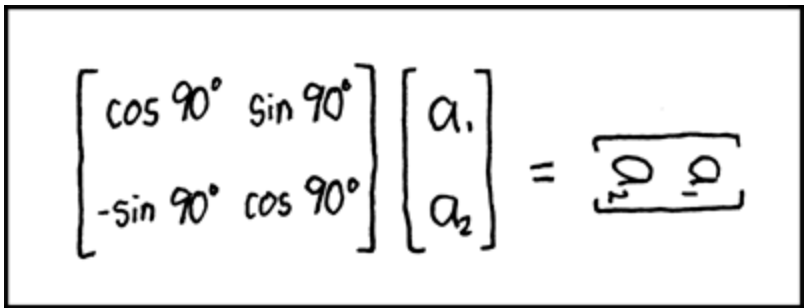
\includegraphics[scale=0.45]{Graphics/rotationmatrix.png}
\end{savequote}
\chapter{Linear Transformations}

    \section{Lecture 30: November 4, 2022}

    \subsection{An Introduction to Linear Transformations}

        Before proceeding into linear transformations, for a review of functions and associated terminology, consult Appendix \ref{appendix:b}. Consider the following definition.
        \begin{definition}{\Stop\,\,Linear Transformations}{lineartransformation}

            Let \(V\) and \(W\) be vector spaces. Let \(F:V\to W\) be a function. Then, \(F\) is a linear transformation if and only if both the following conditions hold:
            \begin{enumerate}
                \item \(\forall \vec{v}_1,\vec{v}_2\in V, F(\vec{v}_1+\vec{v}_2)=F(\vec{v}_1)+F(\vec{v}_2)\).
                \item \(\forall c\in\mathbb{F},\forall\vec{v}\in V, F(c\vec{v})=cF(\vec{v})\).
            \end{enumerate}
            
        \end{definition}
        \vphantom
        \\
        \\
        We remark that a linear transformation ``preserves'' the operations that give structure to the vector spaces involved: vector addition and scalar multiplication.
        \pagebreak
        \\
        \\
        Consider the following examples.
        \begin{example}{\Difficulty\,\Difficulty\,\,Is it a Linear Transformation? 1}{lintrans1}

            Let \(F:\mathcal{M}_{mn}\to \mathcal{M}_{nm}\) where \(F(A)=A^T\). Is \(F\) a linear transformation?
            \\
            \\
            For matrices \(A_1,A_2\in\mathcal{M}_{mn}\) and scalar \(c\in\mathbb{R}\), we have
            \begin{align*}
                F(A_1+A_2)&=(A_1+A_2)^T \\
                &=A_1^T+A_2^T \\
                &=F(A_1)+F(A_2)
            \end{align*}
            and
            \begin{align*}
                F(cA_1)&=(cA_1)^T \\
                &=cA_1^T \\
                &=cF(A_1).
            \end{align*}
            Thus, \(F\) is a linear transformation.
            
        \end{example}
        \begin{example}{\Difficulty\,\Difficulty\,\,Is it a Linear Transformation? 2}{lintrans2}

            Let \(F:\mathcal{P}_n\to\mathcal{P}_{n-1}\) where \(F(\vec{p})=\vec{p}'\), the derivative of \(\vec{p}\). Is \(F\) a linear transformation?
            \\
            \\
            For \(\vec{p}_1,\vec{p}_2\in \mathcal{P}_n\), we know, from Calculus, that the derivative of a sum is the sum of the derivatives, so
            \begin{align*}
                F(\vec{p}_1+\vec{p_2})&=(\vec{p}_1+\vec{p}_2)' \\
                &=\vec{p}_1'+\vec{p}_2' \\
                &=F(\vec{p}_1)+F(\vec{p}_2).
            \end{align*}
            For \(c\in\mathbb{R}\), the constant multiple rule, from Calculus, tells us that
            \begin{align*}
                F(c\vec{p}_1)&=(c\vec{p}_1)' \\
                &=c\vec{p_1}' \\
                &=cF(\vec{p_1}).
            \end{align*}
            Thus, \(F\) is a linear transformation.
        \end{example}
        \pagebreak
        \begin{example}{\Difficulty\,\Difficulty\,\,Is it a Linear Transformation? 3}{lintrans3}

            Let \(F:\mathcal{P}_{n}\to W\) where \(W=\Span\left(\left\{\frac{1}{s},\ldots,\frac{1}{s^{n+1}}\right\}\right)\) and
            \begin{align*}
                F(\vec{p})&=\laplace{\vec{p}(t)}(s) \\
                &=\int_0^\infty e^{-st}\vec{p}(t)\dd t.
            \end{align*}
            Is \(F\) a linear transformation?
            \\
            \\
            For \(\vec{p}_1(t),\vec{p}_2(t)\in\mathcal{P}_n\), we have
            \begin{align*}
                F(\vec{p}_1(t)+\vec{p}_2(t))&=\int_0^\infty e^{-st}(\vec{p}_1(t)+\vec{p}_2(t))\dd t \\
                &=\int_0^\infty e^{-st}\vec{p}_1(t)+e^{-st}\vec{p}_2(t)\dd t \\
                &=\int_0^\infty e^{-st}\vec{p}_1(t)\dd t+\int_0^\infty e^{-st}\vec{p}_2(t)\dd t \\
                &=F(\vec{p}_1(t))+F(\vec{p}_2(t)).
            \end{align*}
            For \(c\in\mathbb{R}\), we have 
            \begin{align*}
                F(c\vec{p}_1(t))&=\int_0^\infty ce^{-st}\vec{p}_1(t)\dd t \\
                &=c\int_0^\infty e^{-st}\vec{p}_1(t)\dd t \\
                &=cF(\vec{p}_1(t)).
            \end{align*}
            Thus, \(F\) is a linear transformation.
        \end{example}
        \pagebreak
        \begin{example}{\Difficulty\,\Difficulty\,\,Is it a Linear Transformation? 4}{lintrans4}

            Let \(V\) be a vector space with \(\dim V=n\). Let \(B\) be an ordered basis for \(V\). Then, every \(\vec{v}\in V\) has coordinatization \([\vec{v}]_B\) with respect to \(B\). Consider the function \(F:V\to\mathbb{R}^n\) given by 
            \begin{equation*}
                F(\vec{v})=[\vec{v}]_B.
            \end{equation*}
            Is \(F\) a linear transformation?
            \\
            \\
            For \(\vec{v}_1,\vec{v}_2\in V\), we have
            \begin{align*}
                F(\vec{v}_1+\vec{v}_2)&=[\vec{v}_1+\vec{v}_2]_B \\
                &=[\vec{v}_1]_B+[\vec{v}_2]_B \\
                &=F(\vec{v}_1)+F(\vec{v}_2),
            \end{align*}
            by Theorem \ref{thm:propcoords}. Then, for \(c\in\mathbb{R}\), we have
            \begin{align*}
                F(c\vec{v}_1)&=[c\vec{v}_1]_B \\
                &=c[\vec{v}_1]_B \\
                &=cF(\vec{v}),
            \end{align*}
            also by Theorem \ref{thm:propcoords}. Thus, \(F\) is a linear transformation.

        \end{example}
        \pagebreak
        \vphantom
        \\
        \\
        We now state some properties of linear transformations.
        \begin{theorem}{\Stop\,\,Properties of Linear Transformations}{proplintrans}

            Let \(V\) and \(W\) be vector spaces, and let \(L:V\to W\) be a linear transformation. Let \(\vec{0}_V\) be the zero vector in \(V\) and \(\vec{0}_W\) be the zero vector in \(W\). Then,
            \begin{enumerate}
                \item \(L(\vec{0}_V)=L(\vec{0}_W)\).
                \begin{proof}
                    Consider \(L(\vec{0}_V)=L(0\vec{0}_V)=0L(\vec{0}_V)=\vec{0}_W\), as desired.
                \end{proof}
                \item \(L(-\vec{v})=-L(\vec{v})\).
                \begin{proof}
                    Consider \(L(-\vec{v})=L(-1\vec{v})=-L(\vec{v})\), as desired.
                \end{proof}
                \item \(L(c_1\vec{v}_1+\cdots+c_n\vec{v}_n)=c_1L(\vec{v}_1)+\cdots+c_nL(\vec{v}_n)\) for \(c_1,\ldots,c_n\in\mathbb{F}\) and \(\vec{v}_1,\ldots,\vec{v}_n\in V\) with \(n\geq2\).
                \begin{proof}
                    We proceed by induction. For the base case when \(n=2\), we have
                    \begin{align*}
                        L(c_1\vec{v}_1+c_2\vec{v}_2)&=L(c_1\vec{v}_1)+L(c_2\vec{v}_2) \\
                        &=c_1L(\vec{v}_1)+c_2L(\vec{v}_2).
                    \end{align*}
                    Then, suppose that for all \(n=k\), 
                    \begin{equation*}
                        L(c_1\vec{v}_1+\cdots+c_k\vec{v}_k)=c_1L(\vec{v}_1)+\cdots+c_kL(\vec{v}_k).
                    \end{equation*}
                    Then, we have
                    \begin{align*}
                        L(c_1\vec{v}_1+\cdots+c_k\vec{v}_k+c_{k+1}v_{k+1})&=c_1L(\vec{v}_1)+\cdots+c_kL(\vec{v}_k)+L(c_{k+1}\vec{v}_{k+1}) \\
                        &=c_1L(\vec{v}_1)+\cdots+c_kL(\vec{v}_k)+c_{k+1}L(\vec{v}_{k+1}),
                    \end{align*}
                    as desired.
                \end{proof}
            \end{enumerate}
            
        \end{theorem}
        \vphantom
        \\
        \\
        We remark that not every function between vector spaces is a linear transformation. To show that some function between vector spaces is not a linear transformation, we must show a counterexample of the conditions in Definition \ref{def:lineartransformation}.
        \pagebreak
        \\
        \\
        We now turn to compositions of linear transformations.
        \begin{theorem}{\Stop\,\,Compositions of Linear Transformations}{compositionslintrans}

            Let \(V_1\), \(V_2\), and \(V_3\) be vector spaces and \(L_1:V_1\to V_2\) and \(L_2:V_2\to V_3\) be linear transformations. Then, \((L_2\circ L_1):V_1\to V_3\) with \((L_2\circ L_1)(\vec{v})=L_2(L_1(\vec{v}))\) is a linear transformation for \(\vec{v}\in V_1\).
            \begin{proof}
                For \(\vec{v}_1,\vec{v}_2\in V_1\), we have
                \begin{align*}
                    (L_2\circ L_1)(\vec{v}_1+\vec{v}_2)&=L_2(L_1(\vec{v}_1+\vec{v}_2)) \\
                    &=L_2(L_1(\vec{v}_1)+L_1(\vec{v}_2)) \\
                    &=L_2(L_1(\vec{v}_1))+L_2(L_1(\vec{v}_2)) \\
                    &=(L_2\circ L_1)(\vec{v}_1)+(L_2\circ L_1)(\vec{v}_2).
                \end{align*}
                Then, for \(c\in\mathbb{F}\), we have
                \begin{align*}
                    (L_2\circ L_1)(c\vec{v}_1)&=L_2(L_1(c\vec{v}_1)) \\
                    &=L_2(cL_1(\vec{v}_1)) \\
                    &=cL_2(L_1(\vec{v}_1)) \\
                    &=c(L_2\circ L_1)(\vec{v}_1),
                \end{align*}
                as desired.
            \end{proof}            
        \end{theorem}
        \vphantom
        \\
        \\
        We now define a special case of linear transformations: linear operators.
        \begin{definition}{\Stop\,\,Linear Operators}{linearoperator}

            Let \(V\) be a vector space. A linear operator on \(V\) is a linear transformation whose domain and codomain are both \(V\).
            
        \end{definition}
        \vphantom
        \\
        \\
        Two special linear operators are the identity linear operator and the zero linear operator. Consider the following definitions.
        \begin{definition}{\Stop\,\,The Identity Linear Operator}{idlinop}

            Let \(V\) be a vector space. Then, the function \(i:V\to V,\vec{v}\mapsto\vec{v}\) is the identity linear operator.
            
        \end{definition}
        \begin{definition}{\Stop\,\,The Zero Linear Operator}{zerolinop}

            Let \(V\) be a vector space. Then, the function \(z:V\to V,\vec{v}\mapsto\vec{0}_V\) is the zero linear operator.
            
        \end{definition}
        \pagebreak
        \vphantom
        \\
        \\
        We end this section with a result about subspaces and linear transformations.
        \begin{theorem}{\Stop\,\,Linear Transformations and Subspaces}{lintranssubspc}

            Let \(L:V\to W\) be a linear transformation. Then,
            \begin{enumerate}
                \item If \(V'\) is a subspace of \(V\), \(L(V')=\{L(\vec{v}):\vec{v}\in V'\}\), the image of \(V'\) in \(W\), is a subspace of \(W\). That is, the range of \(L\) is a subspace of \(W\).
                \begin{proof}
                    We know \(\vec{0}_V\in V'\) since \(V'\) is a subspace. Then, \(\vec{0}_W\in L(V')\) since \(L(\vec{0}_V)=\vec{0}_W\). Next, we take \(\vec{w}_1,\vec{w}_2\in L(V')\). By definition, \(\vec{w}_1=L(\vec{v}_1)\) and \(\vec{w}_2=L(\vec{v}_2)\) for some \(\vec{v}_1,\vec{v}_2\in V'\). Then,
                    \begin{align*}
                        \vec{w}_1+\vec{w}_2&=L(\vec{v}_1)+L(\vec{v}_2) \\
                        &=L(\vec{v}_1+\vec{v}_2).
                    \end{align*}
                    Since \(V'\) is a subspace, \(\vec{v}_1+\vec{v}_2\in V'\). Then, \(\vec{w}_1+\vec{w}_2\) is the image of \(\vec{v}_1+\vec{v}_2\), so \((\vec{w}_1+\vec{w}_2)\in L(V')\). Now, for \(c\in\mathbb{F}\), we have \(c\vec{w}_1=cL(\vec{v}_1)=L(c\vec{v}_1)\). Since \(V'\) is a subspace, \(c\vec{v}_1\in V'\), so \(c\vec{w}_1\) is the image of \(c\vec{v}_1\), so \(c\vec{w}_1\in L(V')\).
                \end{proof}
                \item If \(W'\) is subspace of \(W\), then \(L^{-1}(W')=\{\vec{v}\in V:L(\vec{v})\in W'\}\), the pre-image of \(W'\) in \(V\), is a subspace of \(V\).
                \begin{proof}
                    We know \(\vec{0}_W\in W'\) since \(W'\) is a subspace. Then, \(\vec{0}_V\in L^{-1}(W')\) since \(L(\vec{0}_V)=\vec{0}_W\in W'\). Next, we take \(\vec{v}_1,\vec{v}_2\in L^{-1}(W')\), hence \(L(\vec{v}_1),L(\vec{v}_2)\in W'\). Since \(W'\) is a subspace,
                    \begin{equation*}
                        L(\vec{v}_1)+L(\vec{v}_2)\in W'.
                    \end{equation*}
                    Because \(L\) is linear, \(L(\vec{v}_1)+L(\vec{v}_2)=L(\vec{v}_1+\vec{v}_2)\). Thus, \(L(\vec{v}_1+\vec{v}_2)\in W'\). That is, \((\vec{v}_1+\vec{v}_2)\in L^{-1}(W')\). Finally, for \(c\in\mathbb{F}\), we have \(L(c\vec{v}_1)=cL(\vec{v}_1)\). Since \(W'\) is a subspace and \(L(\vec{v}_1)\in W'\), we have that \(cL(\vec{v}_1)\in W'\). Thus, \(L(c\vec{v}_1)\in W'\) , so \(c\vec{v}_1\in L^{-1}(W')\).
                \end{proof}
            \end{enumerate}
            
        \end{theorem}
        \pagebreak
\section{Lecture 31: November 7, 2022}

    \subsection{Linear Transformations and Bases}

        We begin with an important theorem.
        \begin{theorem}{\Stop\,\,Linear Transformations and Bases}{lineartransformationsbases}

            Let \(B=\{\vec{v}_1,\ldots,\vec{v}_n\}\) be a basis for a vector space \(V\). Let \(W\) be a vector space with arbitrary \(\vec{w}_1,\ldots,\vec{w}_n\in W\). Then, there exists a unique linear transformation \(L:V\to W\) such that
            \begin{equation*}
                L(\vec{v}_1)=\vec{w}_1,\ldots,L(\vec{v}_n)=\vec{w}_n.
            \end{equation*}
            \begin{proof}
                Let \(L:V\to W\) be a linear transformation with
                \begin{equation*}
                    (c_1\vec{v}_1+\cdots+c_n\vec{v}_n)\mapsto(c_1\vec{w}_1+\cdots+c_n\vec{w}_n)
                \end{equation*}
                for scalars \(c_1,\ldots,c_n\). We note that \(L\) is well-defined because \(c_1,\ldots,c_n\) are unique. We will show \(L\) is linear by considering
                \begin{align*}
                    L(\vec{v}+\vec{v}')&=L(c_1\vec{v}_1+\cdots+c_n\vec{v}_n+c_1'\vec{v}_1+\cdots+c_n'\vec{v}_n) \\
                    &=L((c_1+c_1')\vec{v}_1+\cdots+(c_n+c_n')\vec{v}_n) \\
                    &=(c_1+c_1')\vec{w}_1+\cdots+(c_n+c_n')\vec{w}_n \\
                    &=c_1\vec{w}_1+c_1'\vec{w}_1+\cdots+c_n\vec{w}_n+c_2'\vec{w}_n \\
                    &=c_1\vec{w}_1+\cdots+c_n\vec{w}_n+c_1'\vec{w}_1+\cdots+c_n'\vec{w}_n \\
                    &=L(\vec{v})+L(\vec{v}').
                \end{align*}
                We now consider
                \begin{align*}
                    L(c\vec{v})&=L(cc_1\vec{v}_1+\cdots+cc_n\vec{v}_n) \\
                    &=cc_1\vec{w}_1+\cdots+cc_n\vec{w}_n \\
                    &=c(c_1\vec{w}_1+\cdots+c_n\vec{w}_n) \\
                    &=cL(\vec{v}).
                \end{align*}
                Now, we will show that \(L(\vec{v}_i)=\vec{w}_i\). We have that
                \begin{align*}
                    L(\vec{v}_i)&=L(0\vec{v}_1+\cdots+1\vec{v}_i+\cdots+0\vec{v}_n) \\
                    &=\vec{w}_i.
                \end{align*}
                We have shown existence, and now, will show uniqueness. Suppose \(R:V\to W\) is a linear transformation and \(R(\vec{v}_i)=\vec{w}_i\) for \(1\leq i\leq n, i\in \mathbb{N}\). We will show that \(R\) and \(L\) are equal. Let \(\vec{v}\in V\). Then,
                \begin{align*}
                    R(\vec{v})&=R(c_1\vec{v}_1+\cdots+c_n\vec{v}_n) \\
                    &=c_1R(\vec{v}_1)+\cdots+c_nR(\vec{v}_n) \\
                    &=c_1\vec{w}_1+\cdots+c_n\vec{w}_n \\
                    &=L(\vec{v}).
                \end{align*}
                Thus, \(L\) and \(R\) are the same transformation.
            \end{proof}
            
            
        \end{theorem}

\pagebreak

\section{Lecture 32: November 9, 2022}

    \subsection{The Matrix of a Linear Transformation}

        Consider the following theorem. 
        \begin{theorem}{\Stop\,\,Matrices and Linear Transformations}{matlintrans}
            
            Let \(V\) and \(W\) be nontrivial vector spaces. Let \(B=(\vec{v}_1,\ldots,\vec{v}_n)\) and \(C=(\vec{w}_1,\ldots,\vec{w}_m)\) be ordered bases for \(V\) and \(W\), respectively. Let \(L:V\to W\) be a linear transformation. Then, there exists a unique \(A_{BC}\in\mathcal{M}_{mn}\) such that
            \begin{equation*}
                A_{BC}[\vec{v}]_{B}=[L(\vec{v})]_{C}.
            \end{equation*}
            For \(1\leq i\leq n\), the \(i\)th column of \(A_{BC}\) is \([L(\vec{v}_i)]_C\).
            \begin{proof}
                Consider \(A_{BC}\in\mathcal{M}_{mn}\) with \(i\)th column \([L(\vec{v}_i)]_C\), for \(1\leq i\leq n\). We will first show that \(A_{BC}[\vec{v}]_B=[L(\vec{v})]_C\). Suppose that \([\vec{v}]_B=[c_1,\ldots,c_n]\). Then,
                \begin{equation*}
                    \vec{v}=c_1\vec{v}_1+\cdots+c_n\vec{v}_n.
                \end{equation*}
                Then, we have
                \begin{equation*}
                    L(\vec{v})=c_1L(\vec{v}_1)+\cdots+c_nL(\vec{v}_n).
                \end{equation*}
                Next,
                \begin{align*}
                    [L(\vec{v})]_C&=[c_1L(\vec{v}_1)+\cdots+c_nL(\vec{v}_n)]_C \\
                    &=c_1[L(\vec{v}_1)]_C+\cdots+c_n[L(\vec{v}_n)]_C \\
                    &=A_{BC}\begin{bmatrix} c_1 \\ \vdots \\ c_n \end{bmatrix} \\
                    &=A_{BC}[\vec{v}]_B.
                \end{align*}
                Note that the third step in the above transitive chain comes from the fact that the \(i\)th column of \(A_{BC}\) is \([L(\vec{v}_i)]_C\). For uniqueness, suppose \(H\in\mathcal{M}_{nn}\) such that \(H[\vec{v}]_B=[L(\vec{v})]_C\). We can show that \(H=A_{BC}\) if we can show that the \(i\)th column of \(H\) is the \(i\)th column of \(A_{BC}\), or equivalently, \([L(\vec{v}_i)]_C\). Consider \(\vec{v}_i\in B\). We know \([\vec{v}_i]_B=\vec{e}_i\). Then, the \(i\)th column of \(H\) is \(H\vec{e}_i=H[\vec{v}_i]_B=[L(\vec{v}_i)]_C\), which is also the \(i\)th column of \(A_{BC}\).
            \end{proof}
            
        \end{theorem}
        \vphantom
        \\
        \\
        As a remark, Theorem \ref{thm:matlintrans} shows that once we have picked ordered bases for \(V\) and \(W\), each linear transformation \(L:V\to W\) is equivalent to multiplication by a unique corresponding matrix. This matrix, \(A_{BC}\) is called the matrix of the linear transformation \(L\) with respect to the ordered bases \(B\) and \(C\). To compute \(A_{BC}\), we simply apply the linear transformation on each basis element \(\vec{v}_i\), and then express the result with respect to \(C\) to get the respective columns of \(A_{BC}\).
        \pagebreak
        \vphantom
        \\
        \\
        Consider the following example.
        \begin{example}{\Difficulty\,\Difficulty\,\,Finding a Matrix for a Linear Transformation 1}{findmat1}
            
            Consider
            \begin{equation*}
                L:\mathbb{R}^2\to\mathbb{R}^2, \begin{bmatrix} x \\ y \end{bmatrix} \mapsto \begin{bmatrix} x+y \\ x \end{bmatrix}.
            \end{equation*}
            Find the matrix for the linear transformation \(L\) with respect to the ordered bases \(B=([1,0],[0,1])\) and \(C=([1,0],[0,1])\).
            \\
            \\
            Consider
            \begin{align*}
                A_{BC}&=\begin{bmatrix}
                    L\left(\begin{bmatrix} 1 \\ 0 \end{bmatrix}\right) & L\left(\begin{bmatrix} 0 \\ 1 \end{bmatrix}\right)
                \end{bmatrix} \\
                &=\begin{bmatrix}
                    1 & 1 \\
                    1 & 0 \\
                \end{bmatrix}.
            \end{align*}
            Note that we did not have to explicitly coordinatize after finding the image of each element in \(B\) under \(L\) since we are using the standard basis for the codomain as well.
        \end{example}
        \begin{example}{\Difficulty\,\Difficulty\,\,Finding a Matrix for a Linear Transformation 2}{findmat2}
            
            Consider
            \begin{equation*}
                L:\mathbb{R}^2\to\mathbb{R}^2, \begin{bmatrix} x \\ y \end{bmatrix} \mapsto \begin{bmatrix} x+y \\ x \end{bmatrix}.
            \end{equation*}
            Find the matrix for the linear transformation \(L\) with respect to the ordered bases \(B=([1,0],[0,1])\) and \(C=([0,1],[1,0])\).
            \\
            \\
            Consider
            \begin{align*}
                A_{BC}&=\begin{bmatrix}
                    \left[L\left(\begin{bmatrix} 1 \\ 0 \end{bmatrix}\right)\right]_C & \left[L\left(\begin{bmatrix} 0 \\ 1 \end{bmatrix}\right)\right]_C
                \end{bmatrix} \\
                &=\begin{bmatrix}
                    \left[\begin{bmatrix} 1 \\ 1 \end{bmatrix}\right]_C & \left[\begin{bmatrix} 1 \\ 0 \end{bmatrix}\right]_C
                \end{bmatrix} \\
                &=\begin{bmatrix}
                    1 & 0 \\
                    1 & 1
                \end{bmatrix}.
            \end{align*}
            Note that \(L\) is the same linear transformation as the one given in Example \ref{exa:findmat1}; however, we did need to explicitly coordinatize, since we had a nonstandard basis.
        \end{example}
        \pagebreak
        \begin{example}{\Difficulty\,\Difficulty\,\,Finding a Matrix for a Linear Transformation 3}{findmat3}
            
            Consider
            \begin{equation*}
                L:\mathcal{P}_3\to\mathbb{R}^3, c_0+c_1x+c_2x^2+c_3x^3\mapsto[c_0+c_1,2c_2,c_3-c_0].
            \end{equation*}
            Find the matrix for the linear transformation \(L\) with respect to the ordered bases \(B=(x^3,x^2,x,1)\) for \(\mathcal{P}_{3}\) and \(C=([1,0,0],[0,1,0],[0,0,1])\) for \(\mathbb{R}^3\).
            \\
            \\
            By the definition of \(L\), we see that \(L(x^3)=[0,0,1]\), \(L(x^2)=[0,2,0]\), \(L(x)=[1,0,0]\), and \(L(1)=[1,0,-1]\). We need not perform any explicit coordinatization since we are using the standard basis for \(\mathbb{R}^3\), so,
            \begin{equation*}
                A_{BC}=\begin{bmatrix}
                    0 & 0 & 1 & 1 \\
                    0 & 2 & 0 & 0 \\
                    1 & 0 & 0 & -1
                \end{bmatrix}.
            \end{equation*}
            
        \end{example}
        \begin{example}{\Difficulty\,\Difficulty\,\,Finding a Matrix for a Linear Transformation 4}{findmat4}
            
            Consider
            \begin{equation*}
                L:\mathcal{P}_3\to\mathbb{R}^3, c_0+c_1x+c_2x^2+c_3x^3\mapsto[c_0+c_1,2c_2,c_3-c_0].
            \end{equation*}
            Find the matrix for the linear transformation \(L\) with respect to the ordered bases \(B=(x^3+x^2,x^2+x,x+1,1)\) for \(\mathcal{P}_{3}\) and \(C=([-2,1,-3],[1,-3,0],[3,-6,2])\) for \(\mathbb{R}^3\).
            \\
            \\
            By the definition of \(L\), we see that \(L(x^3+x^2)=[0,2,0]\), \(L(x^2+x)=[1,2,0]\), \(L(x+1)=[2,0,-1]\), and \(L(1)=[1,0,-1]\). Now, we must find \([0,2,1]_C\), \([1,2,0]_C\), \([2,0,-1]_C\), and \([1,0,-1]_C\). We consider
            \begin{equation*}
                \begin{bmatrix}
                    -2 & 1 & 3 & | & 0 & 1 & 2 & 1 \\
                    1 & -3 & -6 & | & 2 & 2 & 0 & 0 \\
                    -3 & 0 & 2 & | & 1 & 0 & -1 & -1
                \end{bmatrix}\underbrace{\to}_{\text{RREF}}\begin{bmatrix}
                    1 & 0 & 0 & | & -1 & -10 & -15 & -9 \\
                    0 & 1 & 0 & | & 1 & 26 & 41 & 25 \\
                    0 & 0 & 1 & | & -1 & -15 & -23 & -14
                \end{bmatrix}
            \end{equation*}
            Thus,
            \begin{equation*}
                A_{BC}=\begin{bmatrix}
                    -1 & -10 & -15 & -9 \\
                    1 & 26 & 41 & 25 \\
                    -1 & -15 & -23 & -14
                \end{bmatrix}.
            \end{equation*}
            
        \end{example}
        \pagebreak
        \vphantom
        \\
        \\
        Consider the following theorem.
        \begin{theorem}{\Stop\,\,Matrices for Linear Transformation, Considering Different Bases}{matricesconsdiffbases}
            Let \(V\) and \(W\) be nontrivial vector spaces with \(B\) and \(D\) be distinct ordered bases for \(V\) and \(C\) and \(E\) be distinct ordered bases for \(W\). Suppose \(L:V\to W\) is a linear transformation with matrix \(A_{BC}\). Then,
            \begin{equation*}
                A_{DE}=QA_{BC}P^{-1}
            \end{equation*}
            where \(P\) is the transition matrix from \(B\) to \(D\) and \(Q\) is the transition matrix from \(C\) to \(E\).
            \begin{proof}
                For \(\vec{v}\in V\), consider \(A_{BC}[\vec{v}]_B=[L(\vec{v})]_C\). First, we see that \(P^{-1}[\vec{v}]_D=[\vec{v}]_B\), so we may substitute to obtain \(A_{BC}P^{-1}[\vec{v}]_D=[L(\vec{v})]_C\). If we multiply by \(Q\) on both sides, on the left, we have
                \begin{align*}
                    QA_{BC}P^{-1}[\vec{v}]_D&=Q[L(\vec{v})]_C \\
                    &=[L(\vec{v})]_E.
                \end{align*}
                Since \(A_{DE}\) is the unique matrix such that \(A_{DE}[\vec{v}]_D=[L(\vec{v})]_E\), \(A_{DE}=QA_{BC}P^{-1}\).
            \end{proof}
        \end{theorem}
        \pagebreak
        \vphantom
        \\
        \\
        Consider the following example.
        \begin{example}{\Difficulty\,\Difficulty\,\Difficulty\,\,Finding a Matrix for a Linear Transformation 5}{findmat5}
            
            Consider
            \begin{equation*}
                L:\mathcal{P}_3\to\mathbb{R}^3, c_0+c_1x+c_2x^2+c_3x^3\mapsto[c_0+c_1,2c_2,c_3-c_0].
            \end{equation*}
            As seen in Example \ref{exa:findmat3}, the matrix for \(L\) using the standard bases for \(\mathcal{P}_3\) and \(\mathbb{R}^3\) was
            \begin{equation*}
                A_{BC}=\begin{bmatrix}
                    0 & 0 & 1 & 1 \\
                    0 & 2 & 0 & 0 \\
                    1 & 0 & 0 & -1
                \end{bmatrix},
            \end{equation*}
            where, again \(B=(x^3,x^2,x,1)\) and \(C=([1,0,0],[0,1,0],[0,0,1])\). We will now check our work in Example \ref{exa:findmat4}, where we saw the matrix for \(L\), with respect to the bases \(D=(x^3+x^2,x^2+x,x+1,1)\) and \(E=([-2,1,-3],[1,3,0],[3,-6,2])\) was
            \begin{equation*}
                A_{DE}=\begin{bmatrix}
                    -1 & -10 & -15 & -9 \\
                    1 & 26 & 41 & 25 \\
                    -1 & -15 & -23 & -14
                \end{bmatrix}.
            \end{equation*}
            To calculate the transition matrix \(P^{-1}\) from \(D\) to \(B\), we have
            \begin{equation*}
                \begin{bmatrix}
                    1 & 0 & 0 & 0 & | & 1 & 0 & 0 & 0 \\
                    0 & 1 & 0 & 0 & | & 1 & 1 & 0 & 0 \\
                    0 & 0 & 1 & 0 & | & 0 & 1 & 1 & 0 \\
                    0 & 0 & 0 & 1 & | & 0 & 0 & 1 & 1
                \end{bmatrix},
            \end{equation*}
            so
            \begin{equation*}
                P^{-1}=\begin{bmatrix}
                    1 & 0 & 0 & 0 \\
                    1 & 1 & 0 & 0 \\
                    0 & 1 & 1 & 0 \\
                    0 & 0 & 1 & 1
                \end{bmatrix}.
            \end{equation*}
            To calculate the transition matrix from \(C\) to \(E\), we have
            \begin{equation*}
                \begin{bmatrix}
                    -2 & 1 & 3 & | & 1 & 0 & 0 \\
                    1 & 3 & -6 & | & 0 & 1 & 0 \\
                    -3 & 0 & 2 & | & 0 & 0 & 1
                \end{bmatrix}\underbrace{\to}_\text{RREF}\begin{bmatrix}
                    1 & 0 & 0 & | & -6 & -2 & 3 \\
                    0 & 1 & 0 & | & 16 & 5 & -9 \\
                    0 & 0 & 1 & | & -9 & -3 & 5
                \end{bmatrix}.
            \end{equation*}
            so
            \begin{equation*}
                Q=\begin{bmatrix}
                    -6 & -2 & 3 \\
                    16 & 5 & -9 \\
                    -9 & -3 & 5
                \end{bmatrix}.
            \end{equation*}
            Then,
            \begin{align*}
                A_{DE}=QA_{BC}P^{-1}&=\begin{bmatrix}
                    -6 & -2 & 3 \\
                    16 & 5 & -9 \\
                    -9 & -3 & 5
                \end{bmatrix}\begin{bmatrix}
                    0 & 0 & 1 & 1 \\
                    0 & 2 & 0 & 0 \\
                    1 & 0 & 0 & -1
                \end{bmatrix}\begin{bmatrix}
                1 & 0 & 0 & 0 \\
                1 & 1 & 0 & 0 \\
                0 & 1 & 1 & 0 \\
                0 & 0 & 1 & 1
            \end{bmatrix} \\
            &=\begin{bmatrix}
                -1 & -10 & -15 & -9 \\
                1 & 26 & 41 & 25 \\
                -1 & -15 & -23 & -14
            \end{bmatrix},
            \end{align*}
            as desired.
            
        \end{example}
        \vphantom
        \\
        \\
        We now revisit and consider similar matrices.
        \begin{theorem}{\Stop\,\,Similar Matrices and Linear Operators}{simmatlinops}

            Let \(V\) be a vector space with bases \(C\) and \(D\). Let \(L:V\to V\) be a linear operator, so there exists some \(A_{CC}\) and \(A_{DD}\). Let \(P\) be the transition matrix from \(D\) to \(C\). Then, by Theorem \ref{thm:matricesconsdiffbases}, 
            \begin{equation*}
                A_{CC}=PA_{DD}P^{-1}
            \end{equation*}
            and
            \begin{equation*}
                A_{DD}=P^{-1}A_{CC}P.
            \end{equation*}
            Thus, \(A_{CC}\) and \(A_{DD}\) are similar. Generally, any two matrices for the same linear operator, with respect to different bases, are similar, by Definition \ref{def:similarity}.
             
        \end{theorem}
        \vphantom
        \\
        \\
        Finally, we present an important result about compositions of linear transformations and matrix multiplication.
        \begin{theorem}{\Stop\,\,The Matrix of a Composition of Linear Transformations}{matcomplintrans}

            Let \(V_1\), \(V_2\) and \(V_3\) be nontrivial finite dimensional vector spaces with ordered bases \(B\), \(C\), and \(D\), respectively. Let \(L_1:V_1\to V_2\) be a linear transformation with matrix \(A_{BC}\), and let \(L_2:V_2\to V_3\) be a linear transformation with matrix \(A_{CD}\). Then, the matrix, \(A_{BD}\), for the composite linear transformation \(L_2\circ L_1:V_1\to V_3\), with respect to bases \(B\) and \(D\), is \(A_{CD}A_{BC}\).
            
        \end{theorem}

\pagebreak

\section{Lecture 33: November 11, 2022}

    \subsection{Kernel and Range}

        We now define some important concepts.
        \begin{definition}{\Stop\,\,Kernel}{kernel}

            The kernel of a linear transformation \(L:V\to W\), is given by
            \begin{equation*}
                \ker(L)=\{\vec{v}\in V:L(\vec{v})=\vec{0}_W\}.
            \end{equation*}
            
        \end{definition}
        \begin{definition}{\Stop\,\,Range}{range}

            The range of a linear transformation \(L:V\to W\), is given by
            \begin{equation*}
                \range(L)=\{\vec{w}\in W:\exists\vec{v}\in V, L(\vec{v})=\vec{w}\}.
            \end{equation*}
            
        \end{definition}
        \pagebreak
        \vphantom
        \\
        \\
        Consider the following theorem.
        \begin{theorem}{\Stop\,\,Kernel and Range are Subspaces}{kerransubspc}

            Let \(L:V\to W\) be a linear transformation. Then, \(\ker(L)\) is a subspace of \(V\) and \(\range(L)\) is a subspace of \(W\).
            \begin{proof}
                For \(\ker(L)\), we have \(\vec{0}_V\in\ker(L)\) since \(L(\vec{0}_V)=\vec{0}_W\). Then, for \(\vec{v}_1,\vec{v}_2\in \ker(L)\), we have
                \begin{align*}
                    L(\vec{v}_1+\vec{v}_2)&=L(\vec{v}_1)+L(\vec{v}_2) \\
                    &=\vec{0}_W+\vec{0}_W \\
                    &=\vec{0}_W,
                \end{align*}
                so \(\vec{v}_1+\vec{v}_2\in\ker(L)\). Then, we also have
                \begin{align*}
                    L(c\vec{v}_1)&=cL(\vec{v}_1) \\
                    &=c\vec{0}_W \\
                    &=\vec{0}_W,
                \end{align*}
                for some \(c\in\mathbb{F}\). Thus, \(c\vec{v}_1\in\ker(L)\), as desired. For \(\range(L)\), we have \(\vec{0}_W\in\range(L)\) since \(L(\vec{0}_V)=\vec{0}_W\). Then, if \(\vec{w}_1,\vec{w}_2\in\range(L)\), \(L(\vec{v}_1)=\vec{w}_1\) and \(L(\vec{v}_2)=\vec{w}_2\) for some \(\vec{v}_1,\vec{v}_2\in V\). Then,
                \begin{align*}
                    L(\vec{v}_1+\vec{v}_2)&=L(\vec{v}_1)+L(\vec{v}_2) \\
                    &=\vec{w}_1+\vec{w}_2,
                \end{align*}
                meaning \(\vec{w}_1+\vec{w}_2\in \range(L)\). Then, we also have
                \begin{align*}
                    L(c\vec{v}_1)&=cL(\vec{v}_1) \\
                    &=c\vec{w}
                \end{align*}
                for some \(c\in\mathbb{F}\). Thus, \(c\vec{w}\in\range(L)\), as desired.
            \end{proof}
        
        \end{theorem}
        \pagebreak
        \vphantom
        \\
        \\
        Consider the linear transformation
        \begin{equation*}
            L_A:\mathbb{R}^n\to\mathbb{R}^m, \vec{v}\mapsto A\vec{v}
        \end{equation*}
        for \(A\in\mathcal{A}_{mn}\). Now, we want to find \(\ker(L_A)\) and \(\range(L_A)\). Consider the following theorems.
        \begin{theorem}{\Stop\,\,Finding the Kernel of a Linear Transformation}{findker}

            Let \(A\in\mathcal{M}_{mn}\). Let \(L_A\) be a linear transformation with
            \begin{equation*}
                L_A:\mathbb{R}^n\to\mathbb{R}^m, \vec{v}\mapsto A\vec{v}.
            \end{equation*}
            We find a basis of \(\ker(L)\) by finding particular solutions to \([A|\vec{0}]\). We find each particular solution \(\vec{v}_i\) by setting the \(i\)th free variable in the system to \(1\) and the other free variables to \(0\). We end up with the set \(\{\vec{v}_1,\ldots,\vec{v}_k\}\) as a basis for \(\ker(L)\). Then, \(\ker(L)=\Span(\{\vec{v}_1,\ldots,\vec{v}_k\})\). As a remark, \(\dim(\ker(L))\) is the number of free variables in the homogeneous solution set.
        \end{theorem}
        \begin{theorem}{\Stop\,\,Finding the Range of a Linear Transformation}{findrange}

            Let \(A\in\mathcal{M}_{mn}\). Let \(L_A\) be a linear transformation with
            \begin{equation*}
                L_A:\mathbb{R}^n\to\mathbb{R}^m, \vec{v}\mapsto A\vec{v}.
            \end{equation*}
            To find \(\range(L)\), we need to row reduce \(A\). The columns in \(A\) corresponding to the pivot columns after row reduction is complete form a basis of \(\range(L)\). This is because the span of the columns of \(A\) is \(\range(L)\), and we must then form a basis by keeping only the pivot columns. As a remark, \(\dim(\range(L))=\rank A\), the number of pivot columns.

        \end{theorem}
        \pagebreak
        \vphantom
        \\
        \\
        Consider the following examples.
        \begin{example}{\Difficulty\,\Difficulty\,\,Find Kernel}{findker}

            Let \(L:\mathbb{R}^5\to\mathbb{R}^4,\vec{v}\mapsto A\vec{v}\), where
            \begin{equation*}
                A=\begin{bmatrix}
                    8 & 4 & 16 & 32 & 0 \\
                    4 & 2 & 10 & 22 & -4 \\
                    -2 & -1 & -5 & -11 & 7 \\
                    6 & 3 & 15 & 33 & -7
                \end{bmatrix}.
            \end{equation*}
            Find \(\ker(L)\).
            \\
            \\
            To find \(\ker(L)\), we solve \([A|\vec{0}]\) by row reduction to obtain
            \begin{equation*}
                \begin{bmatrix}
                    1 & \frac{1}{2} & 0 & -2 & 0 & | & 0 \\
                    0 & 0 & 1 & 3 & 0 & | & 0 \\
                    0 & 0 & 0 & 0 & 1 & | & 0 \\
                    0 & 0 & 0 & 0 & 0 & | & 0 
                \end{bmatrix}.
            \end{equation*}
            We see that there are free variables in the second and fourth columns. The solution set to the system is
            \begin{equation*}
                \left\{\left[-\frac{1}{2}c_1+2c_2,c_1,-3c_2,c_2,0\right]:c_1,c_2\in\mathbb{R}\right\}.
            \end{equation*}
            If \(c_1=1\) and \(c_2=0\), we have the particular solution \(\vec{v}_1=[-\frac{1}{2},1,0,0,0]\). If \(c_1=0\) and \(c_2=1\), we have \(\vec{v}_2=[2,0,-3,1,0]\). Thus,
            \begin{equation*}
                \ker(L)=\left\{c_1\left[-\frac{1}{2},1,0,0,0\right]+c_2[2,0,-3,1,0]:c_1,c_2\in\mathbb{R}\right\}.
            \end{equation*}
            It is worth noting that the initial solution set was indeed also \(\ker(L)\), but it is nice to see \(\ker(L)\) as the span of a basis of \(\ker(L)\). We will further simplify to obtain
            \begin{equation*}
                \ker(L)=\left\{c_1\left[-1,2,0,0,0\right]+c_2[2,0,-3,1,0]:c_1,c_2\in\mathbb{R}\right\}.
            \end{equation*}

        \end{example}
        \pagebreak
        \begin{example}{\Difficulty\,\Difficulty\,\,Find Range}{findran}

            Let \(L:\mathbb{R}^5\to\mathbb{R}^4,\vec{v}\mapsto A\vec{v}\), where
            \begin{equation*}
                A=\begin{bmatrix}
                    8 & 4 & 16 & 32 & 0 \\
                    4 & 2 & 10 & 22 & -4 \\
                    -2 & -1 & -5 & -11 & 7 \\
                    6 & 3 & 15 & 33 & -7
                \end{bmatrix}.
            \end{equation*}
            Find \(\range(L)\).
            \\
            \\
            To find \(\range(L)\), row reduce \(A\) to obtain
            \begin{equation*}
                \begin{bmatrix}
                    1 & \frac{1}{2} & 0 & -2 & 0 \\
                    0 & 0 & 1 & 3 & 0 \\
                    0 & 0 & 0 & 0 & 1 \\
                    0 & 0 & 0 & 0 & 0 
                \end{bmatrix}.
            \end{equation*}
            We see that there are pivots in the first, third, and fifth columns. Thus, 
            \begin{equation*}
                \range(L)=\{c_1[8,4,-2,6]+c_2[16,10,-5,15]+c_3[0,-4,7,-7]:c_1,c_2,c_3\in\mathbb{R}\}.
            \end{equation*}
            
        \end{example}
        \pagebreak
        \vphantom
        \\
        \\
        The next theorems combine the results of Theorem \ref{thm:findker} and Theorem \ref{thm:findrange} to find 
        \begin{equation*}
            \dim(\ker(L))+\dim(\range(L)).
        \end{equation*}
        But first, consider the following definitions.
        \begin{definition}{\Stop\,\,Nullity of a Linear Transformation}{nullity}

            Suppose \(V\) and \(W\) are finite dimensional vector spaces and \(L:V\to W\) is a linear transformation. Then,
            \begin{equation*}
                \nullity(L)=\dim(\ker(L)).
            \end{equation*}
            
        \end{definition}
        \begin{definition}{\Stop\,\,Rank of a Linear Transformation}{ranklintrans}

            Suppose \(V\) and \(W\) are finite dimensional vector spaces and \(L:V\to W\) is a linear transformation. Then,
            \begin{equation*}
                \rank(L)=\dim(\range(L)).
            \end{equation*}
            
        \end{definition}
        \vphantom
        \\
        \\
        Now, consider the following theorems.
        \begin{theorem}{\Stop\,\,The Dimension Theorem (The Rank-Nullity Theorem), in \(\mathbb{R}^n\)}{dimthmrn}

            Let \(A\in\mathcal{M}_{mn}\). Let \(L_A\) be a linear transformation with
            \begin{equation*}
                L_A:\mathbb{R}^n\to\mathbb{R}^m, \vec{v}\mapsto A\vec{v}.
            \end{equation*}
            Then,
            \begin{enumerate}
                \item \(\dim(\range(L))=\rank A\).
                \item \(\dim(\ker(L))=n-\rank A\).
                \item \(\dim(\ker(L))+\dim(\range(L))=n\).
            \end{enumerate}
            These results are verified by Theorems \ref{thm:findker} and \ref{thm:findrange}.
            
        \end{theorem}
        \begin{theorem*}{\Stop\,\,The Dimension Theorem (The Rank-Nullity Theorem)}

            Suppose \(V\) and \(W\) are finite dimensional vector spaces and \(L:V\to W\) is a linear transformation. Then,
            \begin{equation*}
                \dim(\ker(L))+\dim(\range(L))=\dim V.
            \end{equation*}
            
        \end{theorem*}
        \vphantom
        \\
        \\
        We will postpone the proof of the above theorem to a later section; hence, we have omitted the reference number.

    \pagebreak

    \subsection{Injections, Surjections, Bijections, and Isomorphisms}

        We state two theorems about if linear transformations are injective or surjective.
        \begin{theorem}{\Stop\,\,Determining Injectivity and Surjectivity}{detinjsurj}

            Suppose \(V\) and \(W\) are finite dimensional vector spaces and \(L:V\to W\) is a linear transformation. Then,
            \begin{enumerate}
                \item The linear transformation \(L\) is injective if and only if \(\ker(L)=\{\vec{0}_V\}\).
                \begin{proof}
                    Suppose \(L\) is injective and let \(\vec{v}\in\ker(L)\). Now, \(L(\vec{v})=\vec{0}_W\). Similarly, \(L(\vec{0}_V)=\vec{0}_W\), and since \(L\) is injective, \(\vec{v}=\vec{0}_V\). Now, we suppose \(\ker(L)=\{\vec{0}_V\}\). We must show \(L\) is injective. Let \(\vec{v}_1,\vec{v}_2\in V\) with \(L(\vec{v}_1)=L(\vec{v}_2)\). We wish to show \(\vec{v}_1=\vec{v}_2\). Now, we have \(L(\vec{v}_1)-L(\vec{v}_2)=\vec{0}_W\), implying that \(L(\vec{v}_1-\vec{v}_2)=\vec{0}_W\). Thus, \(\vec{v}_1-\vec{v}_2\in\ker(L)\). Since \(\ker(L)=\{\vec{0}_V\}\), \(\vec{v}_1-\vec{v}_2=\vec{0}_V\), and so, \(\vec{v}_1=\vec{v}_2\), as desired.
                \end{proof}
                \item The linear transformation \(L\) is surjective if and only if \(\dim(\range(L))=\dim W\).
                \begin{proof}
                    By definition, \(L\) is surjective if and only if \(\range(L)=W\). Then, since \(\range(L)\) is a subspace of \(W\), \(\range(L)=W\) if and only if \(\dim(\range(L))=\dim W\) by Theorem \ref{thm:dimsubspc}.
                \end{proof}
            \end{enumerate}
            
        \end{theorem}
        \begin{theorem}{\Stop\,\,Determining Injectivity and Surjectivity With Equivalent Dimensions}{detinjsurjequivdim}
            
            Suppose \(V\) and \(W\) are finite dimensional vector spaces with \(\dim V=\dim W\). Let \(L:V\to W\) be a linear transformation. Then, \(L\) is injective if and only if \(L\) is surjective.
            \begin{proof}
                We know \(L\) is injective if and only if \(\ker(L)=\{\vec{0}_V\}\), meaning \(\dim (\ker(L))=0\). By the Rank-Nullity Theorem, \(\dim V=\dim(\range(L))+\dim(\ker(L))=\dim(\range(L))\). Since \(\dim V=\dim W\), \(\dim W=\dim(\range(L))\), meaning \(L\) is surjective, by definition. Conversely, if \(L\) is surjective, \(\dim(\ker(L))=0\), meaning that \(\ker(L)=\{\vec{0}_V\}\), which is equivalent to \(L\) being injective.
            \end{proof}

        \end{theorem}
        \pagebreak
        \vphantom
        \\
        \\
        Consider the following examples.
        \begin{example}{\Difficulty\,\Difficulty\,\,Determining Injectivity and Surjectivity 1}{detinjsurj1}

            Consider the linear transformation
            \begin{equation*}
                L:\mathbb{R}^2\to\mathbb{R},\begin{bmatrix} x \\ y \end{bmatrix}\mapsto x+2y.
            \end{equation*}
            Is \(L\) injective? Is \(L\) surjective?
            \\
            \\
            With respect to the standard basis for \(\mathbb{R}^2\), the matrix for \(L\) is
            \begin{equation*}
                A=\begin{bmatrix}
                    1 & 2
                \end{bmatrix}.
            \end{equation*}
            Consider the linear system
            \begin{equation*}
                \begin{bmatrix}
                    1 & 2 & | & 0
                \end{bmatrix},
            \end{equation*}
            with solution set \(\{(-2c,c):c\in\mathbb{R}\}\). Therefore, \(\ker(L)=\{c[-2,1]:c\in\mathbb{R}\}\). Since \(\ker(L)\neq\{\vec{0}\}\), \(L\) is not injective. By the Rank-Nullity Theorem, we have
            \begin{align*}
                \dim(\range(L))&=\dim\mathbb{R}^2-\dim(\ker(L)) \\
                &=2-1=\dim\mathbb{R},
            \end{align*}
            meaning that \(L\) is surjective.
            
        \end{example}
        \begin{example}{\Difficulty\,\Difficulty\,\,Determining Injectivity and Surjectivity 2}{detinjsurj2}

            Consider the linear transformation
            \begin{equation*}
                L:\mathcal{M}_{22}\to\mathbb{R},\begin{bmatrix} a_{11} & a_{12} \\ a_{21} & a_{22} \end{bmatrix}\mapsto a_{11}+a_{22}.
            \end{equation*}
            Is \(L\) injective? Is \(L\) surjective?
            \\
            \\
            With respect to the standard basis for \(\mathcal{M}_{22}\), the matrix for \(L\) is
            \begin{equation*}
                A=\begin{bmatrix}
                    1 & 0 & 0 & 1
                \end{bmatrix}.
            \end{equation*}
            Consider the linear system
            \begin{equation*}
                \begin{bmatrix}
                    1 & 0 & 0 & 1 & | & 0
                \end{bmatrix},
            \end{equation*}
            with solution set \(\{(-c_3,c_1,c_2,c_3):c_1,c_2,c_3\in\mathbb{R}\}\). Therefore, 
            \begin{equation*}
                \ker(L)=\{c_1[0,1,0,0]+c_2[0,0,1,0]+c_3[-1,0,0,1]:c_1,c_2,c_3\in\mathbb{R}\}.
            \end{equation*}     
            Since \(\ker(L)\neq\{\vec{0}\}\), \(L\) is not injective. By the Rank-Nullity Theorem, we have
            \begin{align*}
                \dim(\range(L))&=\dim\mathcal{M}_{22}-\dim(\ker(L)) \\
                &=4-3=\dim\mathbb{R},
            \end{align*}
            meaning that \(L\) is surjective.
            
        \end{example}
        \pagebreak
        \begin{example}{\Difficulty\,\Difficulty\,\,Determining Injectivity and Surjectivity 3}{detinjsurj3}

            Consider the linear transformation
            \begin{equation*}
                L:\mathbb{R}^2\to\mathbb{R}^2,\begin{bmatrix} x \\ y \end{bmatrix}\mapsto \begin{bmatrix} x-y \\ 3y \end{bmatrix}.
            \end{equation*}
            Is \(L\) injective? Is \(L\) surjective?
            \\
            \\
            With respect to the standard basis for \(\mathbb{R}^2\), the matrix for \(L\) is
            \begin{equation*}
                A=\begin{bmatrix}
                    1 & -1 \\
                    0 & 3
                \end{bmatrix}.
            \end{equation*}
            Consider the linear system
            \begin{equation*}
                \begin{bmatrix}
                    1 & -1 & | & 0 \\
                    0 & 3 & | & 0
                \end{bmatrix}.
            \end{equation*}
            Since \(A\) is nonsingular, there exists only a trivial solution for the above system, so \(\ker(L)=\{\vec{0}\}\) and \(L\) is injective. Since the dimensions of the domain and codomain of \(L\) are equal, and \(L\) is injective, \(L\) is surjective.
            
        \end{example}
        \begin{example}{\Difficulty\,\Difficulty\,\Difficulty\,\,Determining Injectivity and Surjectivity 4}{detinjsurj4}

            Consider the linear transformation
            \begin{equation*}
                L:\mathcal{P}\to\mathcal{P},p(x)\mapsto x^2p(x)+xp'(x).
            \end{equation*}
            Is \(L\) injective? Is \(L\) surjective?
            \\
            \\
            Consider the polynomial
            \begin{equation*}
                p(x)=c_0+c_1x+c_2x^2+\cdots+c_nx^n
            \end{equation*}
            with \(c_0,\ldots,c_n\in\mathbb{R}\). Then,
            \begin{align*}
                L(p(x))&=x^2(c_0+c_1x+c_2x^2+\cdots+c_nx^n)+x(c_1+2c_2x+\cdots+nc_nx^{n-1}) \\
                &=c_0x^2+c_1x^3+c_2x^4+\cdots+c_nx^{n+2}+c_1x+2c_2x^2+3c_3x^3+\cdots+nc_nx^n \\
                &=c_1x+(c_0+2c_2)x^2+(c_1+3c_3)x^3+\cdots+(c_{n-3}+(n-1)c_{n-1})\\&\quad+(c_{n-2}+nc_n)x^n+c_{n-1}x^{n+1}+c_nx^{n+2}.
            \end{align*}
            We have expressed \(L(p(x))\) as a finite linear combination of a basis of \(\mathcal{P}\). Therefore, if \(L(p(x))=0\), \(c_1=c_{n-1}=c_n=0\) and \(c_0+2c_2=c_1+3c_3=\cdots=c_{n-2}+nc_n=0\). Since \(c_n=0\), \(c_{n-2}=0\). Similarly, since \(c_{n-1}=0\), \(c_{n-3}=0\). We see that all previous terms \(c_0=\cdots=c_{n-4}=0\) because we can substitute terms we know to be zero into the summation. For example, next, we will have that since \(c_{n-2}=0\), and \(c_{n-4}+(n-2)c_{n-2}\) is a term in the summation, \(c_{n-4}=0\). We will proceed accordingly to find that \(c_0=\cdots=c_n=0\), meaning that \(p(x)=0\). Thus, \(\ker(L)=\{\vec{0}\}\) and \(L\) is injective. Now, we will note that the degree of \(L(p(x))\) is always greater than or equal to \(2\), unless \(p(x)=0\), in which case the degree of \(L(p(x))\) is zero. Thus, there does not exist \(p(x)\) such that \(L(p(x))=1\), and \(L\) is not surjective.
        \end{example}
        \pagebreak
        \vphantom
        \\
        \\
        Consider the following theorem about linear independence and spanning, with regards to linear transformations.
        \begin{theorem}{\Stop\,\,Injectivity Implies Linear Independence, Surjectivity Implies Spanning}{injlinindepsurjspan}

            Suppose \(V\) and \(W\) are vector spaces and \(L:V\to W\) is a linear transformation. Then,
            \begin{enumerate}
                \item If \(L\) is injective, and \(T\) is a linearly independent subset of \(V\), \(L(T)\) is linearly independent in \(W\).
                \begin{proof}
                    Suppose that \(L\) is injective, and \(T\) is a linearly independent subset of \(V\). We wish to show that all finite subsets of \(L(T)\) are linearly independent. Suppose \(\{L(\vec{v}_1),\ldots,L(\vec{v}_n)\}\subseteq L(T)\) for \(\vec{v}_1,\ldots,\vec{v}_n\in T\). Suppose
                    \begin{equation*}
                        c_1L(\vec{v}_1)+\cdots+c_nL(\vec{v}_n)=\vec{0}_W,
                    \end{equation*}
                    which implies 
                    \begin{equation*}
                        L(c_1\vec{v}_1+\cdots+c_n\vec{v}_n)=\vec{0}_W
                    \end{equation*}
                    for scalars \(c_1,\ldots,c_n\). Thus, \((c_1\vec{v}_1+\cdots+c_n\vec{v}_n)\in\ker(L)\). Since \(\ker(L)=\{\vec{0}_V\}\) because \(L\) is injective,
                    \begin{equation*}
                        c_1\vec{v}_1+\cdots+c_n\vec{v}_n=\vec{0}_V.
                    \end{equation*}
                    Since \(\{\vec{v}_1,\ldots,\vec{v}_n\}\subseteq T\) are linearly independent, \(c_1=\cdots=c_n=0\). Thus, \(\{L(\vec{v}_1),\ldots,L(\vec{v}_n)\}\) is linearly independent as well, meaning that \(L(T)\) is linearly independent, as desired.
                \end{proof}
                \item If \(L\) is surjective and \(S\) spans \(V\), \(L(S)\) spans \(W\).
                \begin{proof}
                    Suppose that \(L\) is surjective and \(S\) spans \(V\). We wish to show that all \(\vec{w}\in W\) can be written as a linear combination of vectors in \(L(S)\). Since \(L\) is surjective, there exists \(\vec{v}\in V\) with \(L(\vec{v})=\vec{w}\). Since \(S\) spans \(V\), we have
                    \begin{equation*}
                        \vec{v}=c_1\vec{v}_1+\cdots+c_n\vec{v}_n
                    \end{equation*}
                    for \(\vec{v}_1,\ldots,\vec{v}_n\in S\) and scalars \(c_1,\ldots,c_n\). Then, 
                    \begin{align*}
                        \vec{w}=L(\vec{v})&=L(c_1\vec{v}_1+\cdots+c_n\vec{v}_n) \\
                        &=c_1L(\vec{v}_1)+\cdots+c_nL(\vec{v}_n).
                    \end{align*}
                    We have written arbitrary \(\vec{w}\in W\) as a linear combination of elements in \(L(S)\), so \(L(S)\) spans \(W\), as desired.
                \end{proof}
            \end{enumerate}
            
        \end{theorem}
        \pagebreak
        \vphantom
        \\
        \\
        Consider the following definition.
        \begin{definition}{\Stop\,\,Isomorphisms}{isomorphisms}

            Suppose \(V\) and \(W\) are finite dimensional vector spaces and \(L:V\to W\) is a linear transformation; \(L\) an isomorphism from \(V\) to \(W\) if and only if \(L\) is both injective and surjective, or bijective.
            
        \end{definition}
        \begin{definition}{\Stop\,\,Invertible Linear Transformations}{invtrans}

            Suppose \(V\) and \(W\) are finite dimensional vector spaces and \(L:V\to W\) is a linear transformation. Then, \(L\) is an invertible linear transformation if and only if there exists some function \(M:W\to V\) such that
            \begin{equation*}
                (M\circ L)(\vec{v})=\vec{v}
            \end{equation*}
            for all \(\vec{v}\in V\) and
            \begin{equation*}
                (L\circ M)(\vec{w})=\vec{w}
            \end{equation*}
            for all \(\vec{w}\in W\).
            
        \end{definition}
        \begin{theorem}{\Stop\,\,Isomorphism If And Only If Invertible}{isoinv}
            
            Let \(L:V\to W\) be a linear transformation. Then, \(L\) is an isomorphism if and only if \(L\) is an invertible linear transformation. If \(L\) is invertible, \(L^{-1}\) is also a linear transformation.
            \begin{proof}
                The first part of this theorem follows from Theorem \ref{thm:existinv}, as by definition, \(L\) is an isomorphism if and only if \(L\) is bijective. Now, we just seek to show that \(L^{-1}\) is a linear transformation. First, consider \(\vec{w}_1,\vec{w}_2\in W\). Since \(L\) is surjective, we have \(\vec{w}_1=L(\vec{v}_1)\) and \(\vec{w}_2=L(\vec{v}_2)\) for \(\vec{v}_1,\vec{v}_2\in V\). We have
                \begin{align*}
                    L^{-1}(\vec{w}_1+\vec{w}_2)&=L^{-1}(L(\vec{v}_1)+L(\vec{v}_2)) \\
                    &=L^{-1}(L(\vec{v}_1+\vec{v}_2)) \\
                    &=\vec{v}_1+\vec{v}_2 \\
                    &=L^{-1}(\vec{w}_1)+L^{-1}(\vec{w}_2).
                \end{align*}
                Now, for some \(c\in\mathbb{F}\), we have
                \begin{align*}
                    L^{-1}(c\vec{w}_1)&=L^{-1}(cL(\vec{v}_1)) \\
                    &=cL^{-1}(L(\vec{v}_1)) \\
                    &=c\vec{v}_1 \\
                    &=cL^{-1}(\vec{w}_1),
                \end{align*}
                as desired. Note that for the last step of both transitive chains, we used the fact that \(L\) is injective.
            \end{proof}

        \end{theorem}
        \vphantom
        \\
        \\
        The following theorem allows us to determine whether a linear transformation between finite dimensional vector spaces is an isomorphism, and if so, how to find the inverse.
        \begin{theorem}{\Stop\,\,Finding an Inverse Matrix, if it Exists}{findinv}

            Suppose \(V\) and \(W\) are nontrivial finite dimensional vector spaces with ordered bases \(B\) and \(C\), respectively. Let \(L:V\to W\) be a linear transformation. Then, \(L\) is an isomorphism if and only if the matrix representation \(A_{BC}\) associated to \(L\) is nonsingular. If \(L\) is indeed an isomorphism, the matrix \(A_{CB}\) for \(L^{-1}\) is \(A_{BC}^{-1}\).
            
        \end{theorem}
        \vphantom
        \\
        \\
        Consider the following examples.
        \begin{example}{\Difficulty\,\Difficulty\,\,Find Inverse 1}{findinv1}

            Consider
            \begin{equation*}
                L:\mathbb{R}^2\to\mathbb{R}^2,\begin{bmatrix} x \\ y \end{bmatrix}\mapsto\begin{bmatrix} 3x+y \\ x+y \end{bmatrix}.
            \end{equation*}
            Is \(L\) invertible? If so, find its inverse.
            \\
            \\
            Let \(B\) be an ordered basis of \(\mathbb{R}^2\) with
            \begin{equation*}
                B=\left(\begin{bmatrix} 1 \\ 0 \end{bmatrix}, \begin{bmatrix} 0 \\ 1 \end{bmatrix} \right).
            \end{equation*}
            Then,
            \begin{equation*}
                A_{BB}=\begin{bmatrix} 3 & 1 \\ 1 & 1 \end{bmatrix}.
            \end{equation*}
            Since this matrix is invertible, as \(\det A_{BB}\neq 0\), the inverse is given by
            \begin{align*}
                L^{-1}:\mathbb{R}^2\to\mathbb{R}^2&,\begin{bmatrix} x \\ y \end{bmatrix}\mapsto A_{BB}^{-1}\begin{bmatrix} x \\ y \end{bmatrix} \\
                &,\begin{bmatrix} x \\ y \end{bmatrix}\mapsto \begin{bmatrix} \frac{1}{2} & -\frac{1}{2} \\ -\frac{1}{2} & \frac{3}{2} \end{bmatrix}\begin{bmatrix} x \\ y \end{bmatrix}.
            \end{align*}
        \end{example}
        \pagebreak
        \begin{example}{\Difficulty\,\Difficulty\,\,Find Inverse 2}{findinv2}

            Consider
            \begin{equation*}
                L:\mathbb{R}^3\to\mathbb{R}^3,\begin{bmatrix} x \\ y \\ z \end{bmatrix}\mapsto A\begin{bmatrix} x \\ y \\ z \end{bmatrix}.
            \end{equation*}
            where
            \begin{equation*}
                A=\begin{bmatrix}
                    1 & 0 & 3 \\
                    0 & 1 & 3 \\
                    0 & 0 & 1
                \end{bmatrix}.
            \end{equation*}
            Is \(L\) invertible? If so, find its inverse.
            \\
            \\
            Since this matrix is invertible, as \(\det A_{BB}\neq 0\), the inverse is given by
            \begin{align*}
                L^{-1}:\mathbb{R}^2\to\mathbb{R}^2&,\begin{bmatrix} x \\ y \\ z \end{bmatrix}\mapsto A^{-1}\begin{bmatrix} x \\ y  \\ z \end{bmatrix} \\
                &,\begin{bmatrix} x \\ y \\ z \end{bmatrix}\mapsto \begin{bmatrix} 1 & 0 & -3 \\ 0 & 1 & -3 \\ 0 & 0 & 1 \end{bmatrix}\begin{bmatrix} x \\ y \\ z \end{bmatrix}.
            \end{align*}
        \end{example}
        \pagebreak
        \vphantom
        \\
        \\
        We end with an important, yet unsurprising, theorem.
        \begin{theorem}{\Stop\,\,Isomorphisms Preserve Linear Independence and Span}{isopreslinindepspan}
            
            Let \(V\) and \(W\) be vector spaces, and let \(L:V\to W\) be an isomorphism.
            \begin{enumerate}
                \item If \(T\) is a linearly independent subset of \(V\), \(L(T)\) is linearly independent in \(W\).
                \begin{proof}
                    Because \(L\) is an isomorphism, \(L\) is injective. Therefore, \(L(T)\) is linearly independent in \(W\) by the first part of Theorem \ref{thm:injlinindepsurjspan}.
                \end{proof}
                \item If \(S\) spans \(V\), \(L(S)\) spans \(W\).
                \begin{proof}
                    Because \(L\) is an isomorphism, \(L\) is surjective. Therefore, \(L(S)\) spans \(W\) by the second part of Theorem \ref{thm:injlinindepsurjspan}.
                \end{proof}
                \item If \(B\) is a basis of \(V\), \(L(B)\) is a basis for \(W\).
                \begin{proof}
                    If \(B\) is a basis for \(V\), \(B\) is linearly independent, so \(L(B)\) is linearly independent. We also have that \(\Span(B)=V\), so \(\Span(L(B))=W\). Since \(L(B)\) is linearly independent and spans \(W\), \(L(B)\) is a basis for \(W\).
                \end{proof}
            \end{enumerate}

        \end{theorem}

        \pagebreak

\section{Lecture 34, November 18, 2022}

    \subsection{Isomorphic Vector Spaces}

        We will now define the notion of equivalence of vector spaces.
        \begin{definition}{\Stop\,\,Isomorphic Vector Spaces}{isovec}

            Suppose \(V\) and \(W\) are vector spaces. Then, \(V\) is isomorphic to \(W\), that is, \(V\cong W\), if and only if there exists some linear transformation \(L:V\to W\) that is an isomorphism.
            
        \end{definition}
        \begin{theorem}{\Stop\,\,\(\cong\) is an Equivalence Relation}{isoequivrel}

            Suppose \(V\) and \(W\) are vector spaces. Then, \(\cong\) is an equivalence relation.
            \begin{proof}
                We must show that \(\cong\) is reflexive, symmetric and transitive. Consider the following.
                \begin{enumerate}
                    \item We wish to show \(V\cong V\). Consider the linear transformation \(i:V\to V,\vec{v}\mapsto\vec{v}\), the identity linear operator, defined by Definition \ref{def:idlinop}. We wish to show that \(i:V\to V\) is an isomorphism. Suppose we have \(\vec{v}_1,\vec{v}_2\in V\) such that \(\vec{v}_1\neq\vec{v}_2\). By definition, \(i(\vec{v}_1)=\vec{v}_1\) and \(i(\vec{v}_2)=\vec{v}_2\) meaning \(i(\vec{v}_1)\neq i(\vec{v}_2)\), so \(i\) is injective. Suppose we have \(\vec{w}\in V\). We wish to show there exists some \(\vec{v}\in V\) such that \(i(\vec{v})=\vec{w}\). By definition, \(\vec{v}=\vec{w}\), so \(i\) is surjective. We have found that \(i\) is an isomorphism from \(V\) to \(V\), so \(V\cong V\).
                    \item Suppose \(V\cong W\) via \(L:V\to W\). Because \(L\) is an isomorphism, \(L^{-1}:W\to V\) exists. Since \((L^{-1})^{-1}=L\), \(L^{-1}\) is an isomorphism, and \(W\cong V\).
                    \item Suppose \(V_1 \cong V_2\) via \(L_1:V_1\to V_2\) and \(V_2\cong V_3\) via \(L_2:V_2\to V_3\). We wish to show that \(L_2\circ L_1:V_1\to V_3\) is an isomorphism. Suppose
                    \begin{equation*}
                        (L_2\circ L_1)(\vec{v_1})=L_2(L_1(\vec{v_1}))=(L_2\circ L_1)(\vec{v}_2)=L_2(L_1(\vec{v}_2))
                    \end{equation*}
                    for \(\vec{v}_1,\vec{v}_2\in V_1\). We wish to show \(\vec{v}_1=\vec{v}_2\). Since \(L_2\) is injective, \(L_1(\vec{v}_1)=L_1(\vec{v}_2)\). Then, since \(L_1\) is injective, \(\vec{v}_1=\vec{v}_2\), as desired. Thus, \(L_2\circ L_1\) is injective. Now, suppose we have \(\vec{w}\in V_3\). We wish to show there exists some \(\vec{v}\in V_1\) such that \((L_2\circ L_1)(\vec{v})=L_2(L_1(\vec{v}))=\vec{w}\). Since \(L_2\) is surjective, there exists some \(\hat{v}\in V_2\) such that \(L_2(\hat{v})=\vec{w}\). Since \(L_1\) is surjective, there exists some \(\vec{v}\in V_1\) such that \(L_1(\vec{v})=\hat{v}\). Thus, \((L_2\circ L_1)(\vec{v})=L_2(L_1(\vec{v}))=L_2(\hat{v})=\vec{w}\), so \(L_2\circ L_1\) is surjective. We have shown that \(L_2\circ L_1\) is both injective and surjective, so it is an isomorphism, as desired.
                \end{enumerate}
            \end{proof}

        \end{theorem}
        \pagebreak
        \vphantom
        \\
        \\
        We will now restate the Dimension Theorem, or the Rank-Nullity Theorem, with an accompanying proof.
        \begin{theorem}{\Stop\,\,The Dimension Theorem (The Rank-Nullity Theorem)}{dimensionthm}

            Suppose \(V\) and \(W\) are finite dimensional vector spaces and \(L:V\to W\) is a linear transformation. Then,
            \begin{equation*}
                \dim(\ker(L))+\dim(\range(L))=\dim V.
            \end{equation*}
            \begin{proof}
                Let \(B_{\ker(L)}=\{\vec{u}_1,\ldots,\vec{u}_m\}\) be a basis for \(\ker(L)\). We can extend \(B_{\ker(L)}\) to form a basis for \(V\), \(B_V\), with \(B_V=\{\vec{u}_1,\ldots,\vec{u}_m,\vec{v}_1,\ldots,\vec{v}_n\}\). Note that \(\dim(\ker(L))=m\) and \(\dim V=m+n\). Then, for some \(\vec{v}\in V\), we have
                \begin{equation*}
                    \vec{v}=c_1\vec{u}_1+\cdots+c_m\vec{u}_m+c_{m+1}\vec{v}_1+\cdots+c_n\vec{v}_n
                \end{equation*}
                for \(c_1,\ldots,c_m,c_{m+1},\ldots,c_n\in\mathbb{F}\). If we apply \(L\) to both sides, we have
                \begin{align*}
                    L(\vec{v})&=L(c_1\vec{u}_1+\cdots+c_m\vec{u}_m+c_{m+1}\vec{v}_1+\cdots+c_n\vec{v}_n) \\
                    &=c_1L(\vec{u}_1)+\cdots+c_mL(\vec{u}_m)+c_{m+1}L(\vec{v}_1)+\cdots+c_nL(\vec{v}_n).
                \end{align*}
                Since \(B_{\ker(L)}\) is a basis of \(\ker(L)\), \(L(\vec{u}_1)=\cdots=L(\vec{u_m})=\vec{0}_W\) and we have
                \begin{equation*}
                    L(\vec{v})=c_{m+1}L(\vec{v}_1)+\cdots+c_nL(\vec{v}_n).
                \end{equation*}
                Therefore, since we have written arbitrary \(L(\vec{v})\) as a linear combination of \(L(\vec{v}_1),\ldots,L(\vec{v}_n)\), we have 
                \begin{equation*}
                    \range(L)=\Span(\{L(\vec{v}_1),\ldots,L(\vec{v}_n)\}).
                \end{equation*}
                Consider
                \begin{align*}
                    \vec{0}_W&=b_1L(\vec{v}_1)+\cdots+b_nL(\vec{v}_n) \\
                    &=L(b_1\vec{v}_1+\cdots+b_n\vec{v}_n)
                \end{align*}
                for \(b_1,\ldots,b_n\in\mathbb{F}\). We see that \(b_1\vec{v}_1+\cdots+b_n\vec{v}_n\in\ker(L)\), so
                \begin{equation*}
                    b_1\vec{v}_1+\cdots+b_n\vec{v}_n=d_1\vec{u}_1+\cdots+d_m\vec{u}_m.
                \end{equation*}
                If we subtract the right hand side from both sides, we have
                \begin{equation*}
                    b_1\vec{v}_1+\cdots+b_n\vec{v}_n+(-d_1)\vec{u}_1+\cdots+(-d_m)\vec{u}_m=\vec{0}_V
                \end{equation*}
                Since \(B_V\) is a basis for \(V\), \(B_V\) is linearly independent, so \(b_1=\cdots=b_n=d_1=\cdots=d_m=0\). Since \(b_1=\cdots=b_n=0\), \(B_{\range(L)}:=\{L(\vec{v}_1),\ldots,L(\vec{v}_n)\}\) is linearly independent. Since \(B_{\range(L)}\) both spans \(\range(L)\) and is linearly independent, \(B_{\range(L)}\) is a basis for \(\range(L)\). We see that \(\dim(\range(L))=n\), so
                \begin{align*}
                    \dim V&=m+n \\
                    &=\dim(\ker(L))+\dim(\range(L)),
                \end{align*}
                as desired.

            \end{proof}

        \end{theorem}
        \vphantom
        \\
        \\
        Consider the following important theorems.
        \begin{theorem}{\Stop\,\,Isomorphism Implies Equivalent Dimension}{equivdim}

            Suppose \(V\) and \(W\) are finite dimensional vector spaces. Then, \(V\cong W\) if and only if \(\dim V=\dim W\).
            \begin{proof}
                Suppose \(V\cong W\). Then, there exists some linear transformation \(L:V\to W\) where \(L\) is an isomorphism. Therefore, we have that \(\dim(\range(L))=\dim W\). We also have \(\ker(L)=\{\vec{0}_V\}\), so \(\dim(\ker(L))=0\). Therefore, by Theorem \ref{thm:dimensionthm},
                \begin{align*}
                    \dim V&=\dim(\ker(L))+\dim(\range(L)) \\
                    &=0+\dim W \\
                    &=\dim W.
                \end{align*}
                Now, suppose \(\dim V=\dim W\). Let \(B_V=\{\vec{v}_1,\ldots,\vec{v}_n\}\) be a basis for \(V\) and \(B_W=\{\vec{w}_1,\ldots,\vec{w}_n\}\) be a basis for \(W\). Let 
                \begin{equation*}
                    L:V\to W, c_1\vec{v}_1+\cdots+c_n\vec{v}_n\mapsto c_1\vec{w}_1+\cdots+c_n\vec{w}_n
                \end{equation*}
                for \(c_1,\ldots,c_n\in\mathbb{F}\). Consider arbitrary \(\vec{w}\in W\). We wish to find some \(\vec{v}\in V\) such that \(L(\vec{v})=\vec{w}\) to show that \(L\) is surjective. Under the supposition \(\dim V=\dim W\), \(L\) is an isomorphism if and only if \(L\) is surjective by Theorem \ref{thm:detinjsurjequivdim}. We have
                \begin{equation*}
                    \vec{w}=c_1\vec{w}_1+\cdots+c_n\vec{w}_n.
                \end{equation*}
                By the definition of \(L\), we know
                \begin{equation*}
                    L(c_1\vec{v}_1+\cdots+c_n\vec{v}_n)=c_1\vec{w}_1+\cdots+c_n\vec{w}_n,
                \end{equation*}
                so \(L\) is surjective and is an isomorphism, so \(V\cong W\), as desired.
            \end{proof}
            
        \end{theorem}
        \begin{theorem}{\Stop\,\,All \(n\)-Dimensional Vector Spaces are Isomorphic to \(\mathbb{R}^n\)}{allisorn}
            
            Suppose \(V\) is a finite dimensional vector space with \(\dim V=n\). Then, \(V\cong \mathbb{R}^n\).
            \begin{proof}
                We have that \(\dim V=n\), and we know that \(\dim\mathbb{R}^n=n\), so by Theorem \ref{thm:equivdim}, \(V\cong\mathbb{R}^n\).
            \end{proof}

        \end{theorem}

      %  \begin{example}{\Stop\,\,Find Inverse 1}{findinv1}
%
      %      Consider
      %      \begin{equation*}
       %         L:\mathbb{R}^2\to\mathbb{R}^2,\begin{bmatrix} x \\ y \end{bmatrix}\mapsto\begin{bmatrix} 3x+y \\ x+y \end{bmatrix}.
       %     \end{equation*}
       %     Is \(L\) invertible, if so, find its inverse.
       %     \\
       %     \\
        %    Let \(B\) be an ordered basis of \(\mathbb{R}^2\) with
       %     \begin{equation*}
              % B=\left(\begin{bmatrix} 1 \\ 0 \end{bmatrix}, \begin{bmatrix} 0 \\ 1 \end{bmatrix} \right).
         %   \end{equation*}
          %  Then,
           % \begin{equation*}
             %   [L(\vec{v})]_{BB}=\begin{bmatrix} 3 & 1 \\ 1 & 1 \end{bmatrix}.
            %\end{equation*}
            %Since this matrix is invertible, as \(\det [L(\vec{v})]_{BB} \neq 0\), the inverse is given by
           % \begin{equation*}
            %    L^{-1}:\mathbb{R}^2\to\mathbb{R}^2,\begin{bmatrix} x \\ y \end{bmatrix}\mapsto([L(\vec{v})]_{BB})^{-1}\begin{bmatrix} x \\ y \end{bmatrix}.
           % \end{equation*}
        %\end{example}

    \pagebreak
    \subsection{Diagonalization of Linear Operators}

        Consider the following definitions, similar to the notions discussed in Chapter \ref{chapter:deteigen}, but in the context of linear transformations.
        \begin{definition}{\Stop\,\,Eigenvalues and Eigenvectors}{eigenvaluesandvectorslintrans}

            Suppose \(V\) is a vector space. Let \(L:V\to V\) be a linear operator. A scalar \(\lambda\) is an eigenvalue of \(L\) if and only if there exists \(\vec{v}\in V\), where \(\vec{v}\neq\vec{0}_V\), such that \(L(\vec{v})=\lambda \vec{v}\). If \(\lambda\) is an eigenvalue of \(L\), \(\vec{v}\) is an eigenvector of \(L\) with eigenvalue \(\lambda\). 

        \end{definition}
        \begin{definition}{\Stop\,\,Eigenspace}{eigenspacelintrans}

            Suppose \(V\) is a vector space. Let \(L:V\to V\) be a linear operator. The eigenspace of a given eigenvalue \(\lambda\) is
            \begin{equation*}
                E_\lambda=\{\vec{v}\in V:L(\vec{v})=\lambda \vec{v}\}\cup\{\vec{0}_V\}.
            \end{equation*}
            Note that ``\(\cup\{\vec{0}_V\}\)'' is somewhat redundant, as it will always satisfy the equation. However, the zero vector is never an eigenvector.
        
        \end{definition}
        \vphantom
        \\
        \\
        Our goal is to find all the eigenvalues and eigenspaces of \(L\). Consider the following theorem.
        \begin{theorem}{\Stop\,\,Finding Eigenvectors and Eigenvalues}{findeigenvs}
    
            Let \(L\) be a linear operator on a nontrivial finite dimensional vector space \(V\). Suppose \(A\in\mathcal{M}_{nn}\) is the matrix representation of \(L\) with respect to some ordered basis of \(V\). The scalar \(\lambda\) is an eigenvalue of \(L\) if and only if \(\lambda\) satisfies
            \begin{equation*}
                \det(A-\lambda I_n)=0.
            \end{equation*}
            
        \end{theorem}
        \vphantom
        \\
        \\
        We will now define what it means for a linear operator to be diagonalizable, while also providing a theorem to provide an equivalent condition.
        \begin{definition}{\Stop\,\,Diagonalizability of a Linear Operator}{diaglintrans}

            A linear operator \(L\) on a finite dimensional vector space is diagonalizable if and only if the matrix representation of \(L\) with respect to some ordered basis for \(V\) is a diagonal matrix.
            
        \end{definition}
        \pagebreak
        \begin{theorem}{\Stop\,\,Diagonalizability of a Linear Operator}{diaglintrans}

            Suppose \(L\) is a linear operator on an \(n\)-dimensional vector space \(V\). Then, \(L\) is diagonalizable if and only if there exists a set of \(n\) linearly independent eigenvectors for \(L\).
            \begin{proof}
                Suppose \(L\) is diagonalizable. Then, there exists some ordered basis \(B=(\vec{v}_1,\ldots,\vec{v}_n)\) for \(V\) such that the matrix representation for \(L\) is a diagonal matrix \(D\). Because \(B\) is a basis, \(B\) is linearly independent. We wish to show that each \(\vec{v}_i\in B\), with \(1\leq i\leq n\), is an eigenvector corresponding to some eigenvalue for \(L\). Let \(d_{ii}\) be the \((i,i)\) element of \(D\). For each \(\vec{v}_i\), we have
                \begin{equation*}
                    [L(\vec{v_i})]_B=D[\vec{v_i}]_B=D\vec{e}_i=d_{ii}\vec{e}_i=d_{ii}[\vec{v_i}]_B=[d_{ii}\vec{v}_i]_B.
                \end{equation*}
                We have shown that \(L(\vec{v}_i)=d_{ii}\vec{v}_i\). That is, we have shown that each \(\vec{v}_i\in B\) is an eigenvector of \(L\) with eigenvalue \(d_{ii}\). Thus, \(B\) is a set of \(n\) linearly independent eigenvectors for \(L\). Conversely, suppose \(B=\{\vec{w}_1,\ldots,\vec{w}_n\}\) is a set of \(n\) linearly independent eigenvectors for \(L\), corresponding to eigenvalues \(\lambda_1,\ldots,\lambda_n\). These eigenvalues need not be distinct. We also note that \(B\) is a basis for \(V\), by Theorem \ref{thm:lindim2}. We wish to show that the matrix representation for \(L\), with respect to \(B\) is diagonal. The \(i\)th column for \(A\) is given by
                \begin{equation*}
                    [L(\vec{w}_i)]_B=[\lambda_i\vec{w}_i]_B=\lambda_i[\vec{w}_i]_B=\lambda_i\vec{e}_i.
                \end{equation*}
                Thus, \(A\) is diagonal, and \(L\) is diagonalizable, as desired.
            \end{proof}
        \end{theorem}
        \pagebreak
        \vphantom
        \\
        \\
        Note that Theorem \ref{thm:diaglintrans} requires that we find ``enough'' linearly independent eigenvectors. We now provide a theorem guaranteeing the linear independence of eigenvectors in certain conditions.
        \begin{theorem}{\Stop\,\,Eigenvectors With Distinct Eigenvalues are Linearly Independent}{eigenvecsdisteigenvalslinindep}

            Suppose \(L\) is a linear operator on \(V\). Let \(\lambda_1,\ldots,\lambda_n\) be distinct eigenvalues for \(L\). If \(\vec{v}_1,\ldots,\vec{v}_n\) are eigenvectors for \(L\) corresponding to \(\lambda_1,\ldots,\lambda_n\), respectively, the set \(\{\vec{v}_1,\ldots,\vec{v}_n\}\) is linearly independent.
            \begin{proof}
                
                We proceed by induction on \(n\). For \(n=1\), any eigenvector \(\vec{v}_1\), for any eigenvalue, by definition is nonzero, so \(\{\vec{v}_1\}\) is linearly independent. Suppose that for all \(k\in\mathbb{N}\), the proposition holds. Now, for distinct eigenvalues \(\lambda_1,\ldots,\lambda_{k+1}\). We wish to show that \(\{\vec{v}_1,\ldots,\vec{v}_{k+1}\}\) is linearly independent. Consider
                \begin{equation*}
                    c_1\vec{v}_1+\cdots+c_{k+1}\vec{v}_{k+1}=\vec{0}_V
                \end{equation*}
                for scalars \(c_1,\ldots,c_n\). If we apply \(L\) to both sides, we have
                \begin{align*}
                    L(\vec{0}_V)&=L(c_1\vec{v}_1+\cdots+c_{k+1}\vec{v}_{k+1}) \\
                    &=c_1L(\vec{v}_1)+\cdots+c_{k+1}L(\vec{v}_{k+1})
                \end{align*}
                which implies
                \begin{equation*}
                    c_1\lambda_1\vec{v}_1+\cdots+c_{k+1}\lambda_{k+1}\vec{v}_{k+1}=\vec{0}_V.
                \end{equation*}
                If we multiply \(c_1\vec{v}_1+\cdots+c_{k+1}\vec{v}_{k+1}=\vec{0}_V\) by \(\lambda_{k+1}\), we have
                \begin{equation*}
                    c_1\lambda_{k+1}\vec{v}_1+\cdots+c_{k+1}\lambda_{k+1}\vec{v}_{k+1}=\vec{0}_V=c_1\lambda_1\vec{v}_1+\cdots+c_{k+1}\lambda_{k+1}\vec{v}_{k+1}=\vec{0}_V.
                \end{equation*}
                which we can rewrite as
                \begin{equation*}
                    c_1(\lambda_1-\lambda_{k+1})\vec{v}_1+\cdots+c_k(\lambda_k-\lambda_{k+1})\vec{v}_k=\vec{0}_V
                \end{equation*}
                By the inductive hypothesis,
                \begin{equation*}
                    c_1(\lambda_1-\lambda_{k+1})=\cdots=c_k(\lambda_k-\lambda_{k+1})=0.
                \end{equation*}
                Since \(\lambda_1,\ldots,\lambda_{k+1}\) are distinct, none of the differences in the above equation can be zero, so \(c_1=\cdots=c_k=0\). Thus, for
                \begin{equation*}
                    c_1\vec{v}_1+\cdots+c_{k+1}\vec{v}_{k+1}=\vec{0}_V,
                \end{equation*}
                we have \(c_{k+1}\vec{v}_{k+1}=\vec{0}_V\). Since \(\vec{v}_{k+1}\neq\vec{0}_V\), we have \(c_{k+1}=0\), as desired.
            \end{proof}
            
        \end{theorem}
        \vphantom
        \\
        \\
        Note that Theorem \ref{thm:eigenvecsdisteigenvalslinindep} provides that if \(L\) is a linear operator on an \(n\)-dimensional vector space and \(L\) has \(n\) distinct eigenvalues, \(L\) is diagonalizable. The converse is false.
        \pagebreak
        \\
        \\
        Consider the following theorems and definitions.
        \begin{definition}{\Stop\,\,Algebraic Multiplicity}{algmultdiag}
            
            Let \(L\) be a linear operator on a finite dimensional vector space. Let \(\lambda\) be an eigenvalue for \(L\). Suppose \((x-\lambda)^k\) is the highest power of \(x-\lambda\) that divides the characteristic polynomial of \(L\). Then, \(k\) is the algebraic multiplicity of \(\lambda\).

        \end{definition}
        \begin{definition}{\Stop\,\,Geometric Multiplicity}{geomultdiag}
            
            Let \(L\) be a linear operator on a finite dimensional vector space. Let \(\lambda\) be an eigenvalue for \(L\). Then, \(\dim E_\lambda\) is the geometric multiplicity of \(\lambda\).

        \end{definition}
        \begin{theorem}{\Stop\,\,Algebraic and Geometric Multiplicities and Diagonalizability}{alggeomultdiag}

            Suppose \(V\) is a finite dimensional vector space. Let \(L:V\to V\) be a linear operator. Then, \(L\) is diagonalizable if and only if
            \begin{enumerate}
                \item The sum of the algebraic multiplicities of all eigenvalues of \(L\) is \(\dim V\).
                \item The geometric multiplicity of each eigenvalue is equal to its algebraic multiplicity.
            \end{enumerate}
            Both conditions must be true.

        \end{theorem}
        \begin{theorem}{\Stop\,\,Union and Intersection of Bases for Eigenspaces}{unioninterbaseseigenspc}

            Suppose \(V\) is a finite dimensional vector space. Let \(L:V\to V\) be a linear operator, and let \(B_1,\ldots,B_k\) be bases for eigenspaces \(E_{\lambda_1},\ldots,E_{\lambda_k}\) for \(L\), where \(\lambda_1,\ldots,\lambda_k\) are distinct eigenvalues for \(L\). Then, \(B_i\cap B_j=\emptyset\) for \(1\leq i<j\leq k\), and \(B_1\cup \cdots\cup B_k\) is a linearly independent subset of \(V\).
            
        \end{theorem}
        \begin{theorem}{\Stop\,\,The Process of Diagonalization for Linear Operators}{procdiaglinops}

            Let \(V\) be an \(n\)-dimensional vector space and let \(L:V\to V\) be a linear operator. Consider the following steps.
            \begin{enumerate}
                \item Find a basis, \(C\), for \(V\). Then, find the matrix representation \(A\) of \(L\) with respect to \(C\).
                \item Apply the steps of Theorem \ref{thm:diagonalization} on \(A\) to find the eigenvalues \(\lambda_1,\ldots,\lambda_k\) and a basis in \(\mathbb{R}^n\) for each eigenspace \(E_\lambda\). If \(\left|\bigcup_{i}E_{\lambda_i}\right|<n\), \(L\) is not diagonalizable. Otherwise, let \(Z=(\vec{w}_1,\ldots,\vec{w}_n)=\bigcup_i E_{\lambda_i}\) be an ordered basis for \(\mathbb{R}^n\).
                \item Find an ordered basis \(B=(\vec{v}_1,\ldots,\vec{v}_n)\) of \(V\) such that \([\vec{v}_i]_C=\vec{w}_i\).
                \item Form \(D\) by finding the matrix representation for \(L\) with respect to \(B\).
                \item If needed, form \(P=\begin{bmatrix} [\vec{v}_1]_C & \cdots & [\vec{v}_n]_C \end{bmatrix}=\begin{bmatrix} \vec{w}_1 & \cdots & \vec{w}_n \end{bmatrix}\). Recall \(D=P^{-1}AP\).
            \end{enumerate}

        \end{theorem}

\begin{savequote}

\end{savequote}
\chapter{Orthogonality}

    \section{Lecture 35: November 28, 2022}

    \subsection{Inner Product Spaces}

        Consider the following definition.
        \begin{definition}{\Stop\,\,Inner Products and Inner Product Spaces}{innerprod}

            An \(\mathbb{F}\)-valued inner product on a vector space \(V\) is a function 
            \begin{equation*}
                \langle\cdot,\cdot\rangle:V\times V\to \mathbb{F}
            \end{equation*}
            such that
            \begin{enumerate}
                \item \(\forall\vec{v}\in V,\iprod{\vec{v}}{\vec{v}}\geq 0\).
                \item \(\vec{v}=\vec{0}_V\iff\iprod{\vec{v}}{\vec{v}}=0\).
                \item \(\forall\vec{u},\vec{v}\in V,\iprod{\vec{u}}{\vec{v}}=\bar{\iprod{\vec{v}}{\vec{u}}}\).
                \item \(\forall\vec{u},\vec{v},\vec{w}\in V,\iprod{\vec{u}+\vec{v}}{\vec{w}}=\iprod{\vec{u}}{\vec{w}}+\iprod{\vec{v}}{\vec{w}}\).
                \item \(\forall c\in\mathbb{F},\forall\vec{u},\vec{v}\in V,\iprod{c\vec{u}}{\vec{v}}=c\iprod{\vec{u}}{\vec{v}}\).
            \end{enumerate}
            The pair \((V,\langle\cdot,\cdot\rangle)\) is called an inner product space.
            
        \end{definition}
        \pagebreak
        \vphantom
        \\
        \\
        Consider the following inner product spaces.
        \begin{enumerate}
            \item The pair \((\mathbb{R}^n, \iprod{\vec{u}}{\vec{v}}=\vec{u}\cdot\vec{v}=u_1v_1+\cdots+u_nv_n)\) is a real inner product space.
            \item The pair \((\mathbb{C}^n, \iprod{\vec{u}}{\vec{v}}=\vec{u}\cdot\vec{v}=u_1\bar{v_1}+\cdots+u_n\bar{v_n})\) is a complex inner product space.
            \item The pair 
                \begin{equation*}
                    \left(V,\iprod{\vec{f}}{\vec{g}}=\int_a^b f(x)g(x)\dd x\right)
                \end{equation*}
                is an real inner product space, for 
                \begin{equation*}
                    V=\left\{f:[a,b]\to\mathbb{R}:\forall c\in[a,b], \lim_{x\to c}=f(c)\right\}.
                \end{equation*}
            \item The pair
            \begin{equation*}
                \left(\mathcal{P}_n,\iprod{\vec{p}}{\vec{q}}=\int_{-1}^1 p(x)\bar{q(x)}\dd x\right)
            \end{equation*}
            is a real inner product space.
        \end{enumerate}
        \pagebreak
        \vphantom
        \\
        \\
        Consider the following theorems and definitions.
        \begin{theorem}{\Stop\,\,Properties of Inner Products}{innerprodprops}

            Let \(V\) be an inner product space. Suppose \(\vec{u},\vec{v},\vec{w}\in V\) and \(c\in\mathbb{F}\). Then,
            \begin{enumerate}
                \item \(F:V\to \mathbb{F},\vec{v}\mapsto\iprod{\vec{v}}{\vec{u}}\) is a linear transformation.
                \begin{proof}
                    Consider \(\vec{v}_1,\vec{v}_2\in V\). Then,
                    \begin{align*}
                        F(\vec{v}_1+\vec{v}_2)&=\iprod{\vec{v}_1+\vec{v}_2}{\vec{u}} \\
                        &=\iprod{\vec{v}_1}{u}+\iprod{\vec{v}_2}{\vec{u}} \\
                        &=F(\vec{v}_1)+F(\vec{v}_2).
                    \end{align*}
                    For \(c\in\mathbb{F}\), we have
                    \begin{align*}
                        F(c\vec{v}_1)&=\iprod{c\vec{v}_1}{\vec{u}} \\
                        &=c\iprod{\vec{v}_1}{\vec{u}},
                    \end{align*}
                    as desired.
                \end{proof}
                \item \(\iprod{\vec{0}_V}{\vec{v}}=0=\iprod{\vec{v}}{\vec{0}_V}\).
                \begin{proof}
                    The first equality is derived by the first part since, for all linear transformations \(L\), \(\vec{0}_V\in\ker(L)\). The second equality is derived from conjugate symmetry.
                \end{proof}
                \item \(\iprod{\vec{u}}{\vec{v}+\vec{w}}=\iprod{\vec{u}}{\vec{v}}+\iprod{\vec{u}}{\vec{w}}\).
                \begin{proof}
                    Consider \(\iprod{\vec{u}}{\vec{v}+\vec{w}}=\bar{\iprod{\vec{v}+\vec{w}}{\vec{u}}}=\bar{\iprod{\vec{v}}{\vec{u}}}+\bar{\iprod{\vec{w}}{\vec{u}}}=\iprod{\vec{u}}{\vec{v}}+\iprod{\vec{u}}{\vec{w}}\).
                \end{proof}
                \item \(\iprod{\vec{u}}{c\vec{v}}=\bar{c}\iprod{\vec{u}}{\vec{v}}\).
                \begin{proof}
                    Consider \(\iprod{\vec{u}}{c\vec{v}}=\bar{\iprod{c\vec{v}}{\vec{u}}}=\bar{c}\bar{\iprod{\vec{v}}{\vec{u}}}=\bar{c}\iprod{\vec{u}}{\vec{v}}\).
                \end{proof}
            \end{enumerate}
            
        \end{theorem}
        \begin{definition}{\Stop\,\,Norms}{norms}

            The norm associated to the inner product \(\langle\cdot,\cdot\rangle\) is
            \begin{equation*}
                ||\cdot||:V\to[0,\infty),\vec{v}\mapsto\sqrt{\iprod{\vec{v}}{\vec{v}}}.
            \end{equation*}
            
        \end{definition}
        \pagebreak
        \begin{theorem}{\Stop\,\,Properties of Norms}{propnorm}

            Suppose \(V\) is an inner product space and \(\vec{v}\in V\). Then,
            \begin{enumerate}
                \item \(||\vec{v}||=0\iff\vec{v}=\vec{0}_V\).
                \begin{proof}
                    If \(\vec{v}=\vec{0}_V\), \(||\vec{v}||=\sqrt{\iprod{\vec{v}}{\vec{v}}}=0\). If \(||\vec{v}||=0\), \(\sqrt{\iprod{\vec{v}}{\vec{v}}}=\iprod{\vec{v}}{\vec{v}}=0\), meaning that \(\vec{v}=\vec{0}_V\).
                \end{proof}
                \item \(\forall c\in\mathbb{F},||c\vec{v}||=|c|||\vec{v}||\).
                \begin{proof}
                    Consider
                    \begin{align*}
                        ||c\vec{v}||&=\sqrt{\iprod{c\vec{v}}{c\vec{v}}} \\
                        &=\sqrt{c\bar{c}\iprod{\vec{v}}{\vec{v}}} \\
                        &=\sqrt{|c|^2\iprod{\vec{v}}{\vec{v}}} \\
                        &=|c|\sqrt{\iprod{\vec{v}}{\vec{v}}} \\
                        &=|c|||\vec{v}||,
                    \end{align*}
                    as desired.
                \end{proof}
            \end{enumerate}
            
        \end{theorem}
        \vphantom
        \\
        \\
        We will now present some generalized proofs of theorems we covered special cases of in Chapter~\ref{chapter:vecmat}. 
        \begin{theorem}{\Stop\,\,The Cauchy-Schwarz Inequality}{cauchyschwarzgen}
            Let \(V\) be an inner product space with \(\vec{v},\vec{w}\in V\). Then,
            \begin{equation*}
                \left|\iprod{\vec{v}}{\vec{w}}\right|\leq||\vec{v}||||\vec{w}||.
            \end{equation*}
            \begin{proof}
                If \(\vec{w}=\vec{0}_V\), the statement is trivial since both sides are zero. We have that for all \(t\in\mathbb{F}\),
                \begin{align*}
                    0&\leq||\vec{v}-t\vec{w}||^2 \\
                    &=\iprod{\vec{v}-t\vec{w}}{\vec{v}-t\vec{w}} \\
                    &=\iprod{\vec{v}}{\vec{v}-t\vec{w}}-t\iprod{\vec{w}}{\vec{v}-t\vec{w}} \\
                    &=||\vec{v}||^2-t\iprod{\vec{w}}{\vec{v}}-\bar{t}\iprod{\vec{v}}{\vec{w}}+|t|^2||\vec{w}||^2.
                \end{align*}
                The quadratic has a minimum at \(t=\frac{\iprod{\vec{v}}{\vec{w}}}{||\vec{w}||^2}=\frac{\bar{\iprod{\vec{w}}{\vec{v}}}}{||\vec{w}||^2}\) and the inequality should hold. The inequality for this \(t\) is
                \begin{equation*}
                    0\leq||\vec{v}||^2-\frac{\iprod{\vec{v}}{\vec{w}}^2}{||\vec{w}||^2}.
                \end{equation*}
                Thus, \(\left|\iprod{\vec{v}}{\vec{w}}\right|^2\leq||\vec{v}||||\vec{w}||^2\implies\left|\iprod{\vec{v}}{\vec{w}}\right|\leq||\vec{v}||||\vec{w}||\).
            \end{proof}
        \end{theorem}
        \pagebreak
        \begin{theorem}{\Stop\,\,The Triangle Inequality}{triineqgen}

            Let \(V\) be an inner product space with \(\vec{v},\vec{w}\in V\). Then,
            \begin{equation*}
                ||\vec{v}+\vec{w}||\leq||\vec{v}||+||\vec{w}||.
            \end{equation*}
            \begin{proof}
                We have
                \begin{align*}
                    ||\vec{v}+\vec{w}||^2&=\iprod{\vec{v}+\vec{w}}{\vec{v}+\vec{w}} \\
                    &=\iprod{\vec{v}}{\vec{v}}+\iprod{\vec{v}}{\vec{w}}+\iprod{\vec{w}}{\vec{v}}+\iprod{\vec{w}}{\vec{w}} \\
                    &\leq\iprod{\vec{v}}{\vec{v}}+\iprod{\vec{w}}{\vec{w}}+2\left|\iprod{\vec{v}}{\vec{w}}\right| \\
                    &\leq\iprod{\vec{v}}{\vec{v}}+\iprod{\vec{w}}{\vec{w}}+2||\vec{v}||||\vec{w}|| \\
                    &=(||\vec{v}||+||\vec{w}||)^2,
                \end{align*}
                as desired.
            \end{proof}

        \end{theorem}
        \vphantom
        \\
        \\
        We now provide notions of distance and angle.
        \begin{definition}{\Stop\,\,Distance}{distance}

            Let \(V\) be an inner product space. The distance betwen \(\vec{v},\vec{w}\in V\) is \(||\vec{v}-\vec{w}||\).
            
        \end{definition}
        \begin{definition}{\Stop\,\,Angle}{angle}

            Let \(V\) be a real inner product space. That is, \(\mathbb{F}=\mathbb{R}\). The angle between \(\vec{v}\neq\vec{0}_V\) and \(\vec{w}\neq\vec{0}_V\) is given by
            \begin{equation*}
                \theta =\arccos\left(\frac{\langle\vec{v},\vec{w}\rangle}{||\vec{v}||||\vec{w}||}\right)
            \end{equation*}
            
        \end{definition}
        \begin{definition}{\Stop\,\,Orthogonality}{orthogonality}

            Let \(V\) be an inner product space. Then, 
            \begin{enumerate}
                \item \(\vec{v},\vec{w}\in V\) are orthogonal if and only if \(\langle\vec{v},\vec{w}\rangle=0\).
                \item A set \(S\subseteq V\) is orthogonal if and only if for each \(\vec{v},\vec{w}\in S\), \(\langle\vec{v},\vec{w}\rangle=0\).
                \item A set \(S\subseteq V\) is orthonormal if and only if it is orthogonal and each \(\vec{v}\in S\) has \(||\vec{v}||=1\).
            \end{enumerate}

        \end{definition}
        \vphantom
        \\
        \\
        Consider the following example.
        \begin{example}{\Difficulty\,\,The Standard Basis of \(\mathbb{F}^n\)}{stdbasisfn}

            The set \(\{\vec{e}_1,\ldots,\vec{e}_n\}\) is orthonormal when considered as a subset of \(\mathbb{R}^n\) or \(\mathbb{C}^n\).
            
        \end{example}
        \pagebreak
        
    \subsection{Orthonormal Bases and the Gram-Schmidt Process}

        Consider the following theorems and definitions.
        \begin{theorem}{\Stop\,\,Orthonormal Implies Linearly Independent}{orthlinindep}
            
            If \(\{\vec{v}_1,\ldots,\vec{v}_n\}\) is orthonormal in an inner product space \(V\), \(\{\vec{v}_1,\ldots,\vec{v}_n\}\) is linearly independent.
            \begin{proof}
                Suppose
                \begin{equation*}
                    c_1\vec{v}_1+\cdots+c_n\vec{v}_n=\vec{0}_V
                \end{equation*}
                for some \(c_1,\ldots,c_n\in\mathbb{F}\). We must show \(c_1=\cdots=c_n=0\). For each \(i\), \(1\leq i\leq n\), consider 
                \begin{align*}
                    0&=\langle c_1\vec{v}_1+\cdots+c_n\vec{v}_n,\vec{v}_i \rangle \\
                    &=\langle c_1\vec{v}_1,\vec{v}_i\rangle+\cdots+\langle c_n\vec{v}_n,\vec{v}_i\rangle \\
                    &=c_1\langle \vec{v}_1,\vec{v}_i\rangle+\cdots+c_n\langle \vec{v}_n,\vec{v}_i\rangle \\
                    &=c_i\langle \vec{v}_i,\vec{v}_i\rangle
                \end{align*}
                We see that \(\langle\vec{v}_i,\vec{v}_i\rangle>0\), since \(\vec{v}_i\neq\vec{0}_V\). We have \(0=c_i||\vec{v}_i||^2\), implying that \(c_i=0\) for each \(i\).
            \end{proof}
            The converse is false.

        \end{theorem}
        \begin{definition}{\Stop\,\,Orthogonal Bases}{orthogonalbasis}

            A set \(B\subseteq V\) is an orthogonal basis if and only if \(B\) is a basis of \(V\) and \(B\) is orthogonal.
            
        \end{definition}
        \begin{definition}{\Stop\,\,Orthonormal Bases}{orthonormalbasis}

            A set \(B\subseteq V\) is an orthonormal basis if and only if \(B\) is a basis of \(V\) and \(B\) is orthonormal.
            
        \end{definition}
        \pagebreak
        \vphantom
        \\
        \\
        We would like to form an orthogonal set of \(n\) vectors from any linearly independent set of \(n\) vectors such that both sets span the same subspace. We present the Gram-Schmidt process.
        \begin{theorem}{\Stop\,\,The Gram-Schmidt Process}{gramschmidt}
            
            Let \(S_1=\{\vec{w}_1,\ldots,\vec{w}_n\}\) be linearly independent. The set \(S_2=\{\vec{v}_1,\ldots,\vec{v}_n\}\) given below is orthogonal, and \(\Span(S_1)=\Span(S_2)\).
            \begin{itemize}
                \item Let \(\vec{v}_1=\vec{w}_1\).
                \item Let \(\vec{v}_2=\vec{w}_2-\left(\frac{\iprod{\vec{w}_2}{\vec{v}_1}}{\iprod{\vec{v}_1}{\vec{v}_1}}\right)\vec{v}_1\).
                \item Let \(\vec{v}_3=\vec{w}_3-\left(\frac{\iprod{\vec{w}_3}{\vec{v}_1}}{\iprod{\vec{v}_1}{\vec{v}_1}}\right)\vec{v}_1-\left(\frac{\iprod{\vec{w}_3}{\vec{v}_2}}{\iprod{\vec{v}_2}{\vec{v}_2}}\right)\vec{v}_2\).
                \item Continue.
                \item Let \(\vec{v}_n=\vec{w}_n-\left(\frac{\iprod{\vec{w}_n}{\vec{v}_1}}{\iprod{\vec{v}_1}{\vec{v}_1}}\right)\vec{v}_1-\left(\frac{\iprod{\vec{w}_n}{\vec{v}_2}}{\iprod{\vec{v}_2}{\vec{v}_2}}\right)\vec{v}_2-\cdots-\left(\frac{\iprod{\vec{w}_n}{\vec{v}_{n-1}}}{\iprod{\vec{v}_{n-1}}{\vec{v}_{n-1}}}\right)\vec{v}_{n-1}\).
            \end{itemize}

        \end{theorem}
        \vphantom
        \\
        \\
        Consider the following examples.
        \begin{example}{\Difficulty\,\Difficulty\,\,Gram-Schmidt 1}{gramschmidt1}

            Apply the Gram-Schmidt process to \(\{[1,1,0,0],[1,1,0,-1]\}\subseteq\mathbb{R}^4\).
            \\
            \\
            Let \(\vec{v}_1=[1,1,0,0]\). Then,
            \begin{align*}
                v_2&=[1,1,0,-1]-\frac{\iprod{[1,1,0,-1]}{[1,1,0,0]}}{\iprod{[1,1,0,0]}{[1,1,0,0]}}[1,1,0,0] \\
                &=[1,1,0,-1]-\frac{2}{2}[1,1,0,0] \\
                &=[0,0,0,-1].
            \end{align*}
            Let \(S=\{[1,1,0,0],[0,0,0,-1]\}\). Then, \(\Span(S)=\Span(\{[1,1,0,0],[1,1,0,-1]\})\).
            
        \end{example}
        \pagebreak
        \begin{example}{\Difficulty\,\Difficulty\,\,Gram-Schmidt 2}{gramschmidt2}

            Apply the Gram-Schmidt process to \(\{[i,-i,1,1],[i,0,0,1],[0,1,-i,0]\}\subseteq\mathbb{C}^4\).
            \\
            \\
            Let \(\vec{v}_1=[i,-i,1,1]\). Then,
            \begin{align*}
                \vec{v}_2&=[i,0,0,1]-\frac{\iprod{[i,0,0,1]}{[i,-i,1,1]}}{\iprod{[i,-i,1,1]}{[i,-i,1,1]}}[i,-i,1,1] \\
                &=[i,0,0,1]-\frac{1}{2}[i,-i,1,1] \\
                &=\left[\frac{1}{2}i,\frac{1}{2}i,-\frac{1}{2},\frac{1}{2}\right].
            \end{align*}
            Then,
            \begin{align*}
                \vec{v}_3&=[0,1,-i,0]-\frac{\iprod{[0,1,-i,0]}{[i,-i,1,1]}}{\iprod{[i,-i,1,1]}{[i,-i,1,1]}}[i,-i,1,1]\\&\quad-\frac{\iprod{[0,1,-i,0]}{[i,-i,1,1]}}{\iprod{\left[\frac{1}{2}i,\frac{1}{2}i,-\frac{1}{2},\frac{1}{2}\right]}{\left[\frac{1}{2}i,\frac{1}{2}i,-\frac{1}{2},\frac{1}{2}\right]}}\left[\frac{1}{2}i,\frac{1}{2}i,-\frac{1}{2},\frac{1}{2}\right] \\
                &=[0,1,-i,0].
            \end{align*}
            Let \(S=\left\{[i,-i,1,1],\left[\frac{1}{2}i,\frac{1}{2}i,-\frac{1}{2},\frac{1}{2}\right],[0,1,-i,0]\right\}\). Then, 
            \begin{equation*}
                \Span(S)=\Span(\{[i,-i,1,1],[i,0,0,1],[0,1,-i,0]\}).
            \end{equation*}

        \end{example}
        \pagebreak
        \begin{example}{\Difficulty\,\Difficulty\,\,Gram-Schmidt 3}{gramschmidt3}
            
            Apply the Gram-Schmidt process to \(\{1,x,x^2\}\subseteq\mathcal{P}\) with inner product given by
            \begin{equation*}
                \iprod{p(x)}{q(x)}=\int_0^1 p(x)q(x) \dd x.
            \end{equation*}
            Let \(\vec{v}_1=1\). Then,
            \begin{align*}
                \vec{v}_2&=x-\frac{\iprod{x}{1}}{\iprod{1}{1}}1 \\
                &=x-\frac{1}{2}.
            \end{align*}
            Then,
            \begin{align*}
                \vec{v}_3&=x^2-\frac{\iprod{x^2}{1}}{\iprod{1}{1}}1-\frac{\iprod{x^2}{x-\frac{1}{2}}}{\iprod{x-\frac{1}{2}}{x-\frac{1}{2}}}\left(x-\frac{1}{2}\right) \\
                &=x^2-\frac{1}{3}-\frac{\frac{1}{4}-\frac{1}{6}}{\frac{\left(1-\frac{1}{2}\right)^3-\left(0-\frac{1}{2}\right)^3}{3}}\left(x-\frac{1}{2}\right) \\
                &=x^2-\frac{1}{3}-\frac{\frac{1}{4}}{\frac{1}{4}}\left(x-\frac{1}{2}\right) \\
                &=x^2-x+\frac{1}{6}.
            \end{align*}
            Let \(S=\left\{1,x-\frac{1}{2},x^2-x+\frac{1}{6}\right\}\). Then,
            \begin{equation*}
                \Span(S)=\Span(\{1,x,x^2\}).
            \end{equation*}
            
        \end{example}
        \vphantom
        \\
        \\
        We can also normalize an orthogonal set into an orthonormal one by just dividing each \(\vec{v}_i\) by \(||\vec{v}_i||\).
        \begin{theorem}{\Stop\,\,Every Inner Product Space Has an Orthonormal Basis}{innerproductspaceorthobasis}

            Every inner product space has an orthonormal basis.
            \begin{proof}
                Suppose \(V\) is a finite dimensional inner product space. Let \(B=\{\vec{w}_1,\ldots,\vec{w}_n\}\) be a basis for \(V\). Apply the Gram-Schmidt process to find orthogonal \(C=\{\vec{v}_1,\ldots,\vec{v}_n\}\) and normalize it. This set is orthonormal and, therefore, linearly independent, and \(\Span(B)=V=\Span(C)\).
            \end{proof}
            
        \end{theorem}
        \pagebreak
        \begin{example}{\Difficulty\,\Difficulty\,\,Finding an Orthonormal Basis}{findorthnormbasis}

            Let \(W=\{[x,y,z,w]:x+y-z-w=0;x,y,z,w\in\mathbb{C}\}\). Find an orthonormal basis for \(W\).
            \\
            \\
            By the membership condition of \(W\), we can rewrite it as
            \begin{equation*}
                W=\{[x,y,z,x+y-z]:x,y,z,w\in\mathbb{C}\}.
            \end{equation*}
            We note that \([1,-1,0,0],[1,0,1,0],[1,1,1,1]\in W\). Let \(B_\neg=\{[1,-1,0,0],[1,0,1,0],[1,1,1,1]\}\). Consider
            \begin{equation*}
                \begin{bmatrix}
                    1 & -1 & 0 & 0 \\
                    1 & 0 & 1 & 0 \\
                    1 & 1 & 1 & 1
                \end{bmatrix}\underbrace{\to}_\text{RREF}
                \begin{bmatrix}
                    1 & 0 & 0 & 1 \\
                    0 & 1 & 0 & 1 \\
                    0 & 0 & 1 & -1
                \end{bmatrix}
            \end{equation*}
            implying that \(\Span(B_\neg)=\{[c_1,c_2,c_3,c_1+c_2-c_3]:c_1,c_2,c_3\in\mathbb{C}\}=W\). Now, consider
            \begin{equation*}
                \begin{bmatrix}
                    1 & 1 & 1 \\
                    -1 & 0 & 1 \\
                    0 & 1 & 1 \\
                    0 & 0 & 1
                \end{bmatrix}\underbrace{\to}_\text{RREF}
                \begin{bmatrix}
                    1 & 0 & 0 \\
                    0 & 1 & 0 \\
                    0 & 0 & 1 \\
                    0 & 0 & 0
                \end{bmatrix},
            \end{equation*}
            implying that \(B_\neg\) is linearly independent and therefore a basis for \(W\). Now, we apply the Gram-Schmidt process to obtain an orthogonal basis. Let \(\vec{v}_1=[1,-1,0,0]\). Then,
            \begin{align*}
                \vec{v}_2&=[1,0,1,0]-\frac{\iprod{1,0,1,0}{[1,-1,0,0]}}{\iprod{[1,-1,0,0]}{[1,-1,0,0]}}[1,-1,0,0] \\
                &=[1,0,1,0]-\frac{1}{2}[1,-1,0,0] \\
                &=\left[\frac{1}{2},\frac{1}{2},1,0\right].
            \end{align*}
            Then,
            \begin{align*}
                \vec{v}_3&=[1,1,1,1]-\frac{\iprod{[1,1,1,1]}{[1,-1,0,0]}}{\iprod{1,-1,0,0}{1,-1,0,0}}[1,-1,0,0]-\frac{\iprod{[1,1,1,1]}{\left[\frac{1}{2},\frac{1}{2},1,0\right]}}{\iprod{\left[\frac{1}{2},\frac{1}{2},1,0\right]}{\left[\frac{1}{2},\frac{1}{2},1,0\right]}}\left[\frac{1}{2},\frac{1}{2},1,0\right] \\
                &=[1,1,1,1]-\frac{4}{3}\left[\frac{1}{2},\frac{1}{2},1,0\right] \\
                &=\left[\frac{1}{3},\frac{1}{3},-\frac{1}{3},1\right].
            \end{align*}
            Our orthogonal basis for \(W\) is then \(B_\perp=\left\{[1,-1,0,0],\left[\frac{1}{2},\frac{1}{2},1,0\right],\left[\frac{1}{3},\frac{1}{3},-\frac{1}{3},1\right]\right\}\). To find an orthonormal basis, we simply normalize each vector to obtain
            \begin{align*}
                B_{\hat{\perp}}&=\left\{\left[\frac{\sqrt{2}}{2},-\frac{\sqrt{2}}{2},0,0\right],\left[\frac{\sqrt{6}}{6},\frac{\sqrt{6}}{6},\frac{\sqrt{6}}{3},0\right],\left[\frac{\sqrt{3}}{6},\frac{\sqrt{3}}{6},-\frac{\sqrt{3}}{6},\frac{\sqrt{3}}{2}\right]\right\}.
            \end{align*}
        \end{example}
        \pagebreak
        \vphantom
        \\
        \\
        We have mentioned many methods of finding orthogonal and orthonormal bases and spanning sets. The following theorems illustrate the utility of doing so.
        \begin{theorem}{\Stop\,\,Coordinatization With Respect to an Orthogonal Basis}{coordsorthogonal}

            Let \(V\) be a finite dimensional inner product space. Let \(W\) be a subspace of \(V\). Suppose \(B=(\vec{v}_1,\ldots,\vec{v}_n)\) is a nonempty ordered orthogonal basis for \(W\). Then, for all \(\vec{w}\in W\),
            \begin{equation*}
                [\vec{w}]_B=\left[\frac{\iprod{\vec{w}}{\vec{v}_1}}{\iprod{\vec{v}_1}{\vec{v}_1}},\ldots,\frac{\iprod{\vec{w}}{\vec{v}_n}}{\iprod{\vec{v}_n}{\vec{v}_n}}\right].
            \end{equation*}
            \begin{proof}
                We know that \([\vec{w}]_B=[c_1,\ldots,c_n]\) for \(c_1,\ldots,c_n\in\mathbb{F}\). We wish to show that for each \(c_i\), with \(1\leq i\leq n\),
                \begin{equation*}
                    c_i=\frac{\iprod{\vec{w}}{\vec{v}_i}}{\iprod{\vec{v}_i}{\vec{v}_i}}.
                \end{equation*}
                We have that
                \begin{equation*}
                    \vec{w}=c_1\vec{v}_1+\cdots+c_n\vec{v}_n.
                \end{equation*}
                Then,
                \begin{align*}
                    \iprod{\vec{w}}{\vec{v}_i}&=\iprod{c_1\vec{v}_1+\cdots+c_n\vec{v}_n}{\vec{v}_i} \\
                    &=c_1\iprod{\vec{v}_1}{\vec{v}_i}+\cdots+c_n\iprod{\vec{v}_n}{\vec{v}_i} \\
                    &=c_i\iprod{\vec{v}_i}{\vec{v}_i}.
                \end{align*}
                Therefore,
                \begin{equation*}
                    c_i=\frac{\iprod{\vec{w}}{\vec{v}_i}}{\iprod{\vec{v}_i}{\vec{v}_i}},
                \end{equation*}
                as desired.
            \end{proof}
        \end{theorem}
        \begin{theorem}{\Stop\,\,Coordinatization With Respect to an Orthonormal Basis}{coordsorthonormal}

            Let \(V\) be a finite dimensional inner product space. Let \(W\) be a subspace of \(V\). Suppose \(B=(\vec{v}_1,\ldots,\vec{v}_n)\) is a nonempty ordered orthonormal basis for \(W\). Then, for all \(\vec{w}\in W\),
            \begin{equation*}
                [\vec{w}]_B=\left[\iprod{\vec{w}}{\vec{v}_1},\ldots,\iprod{\vec{w}}{\vec{v}_n}\right].
            \end{equation*}
            \begin{proof}
                If \(B\) is orthonormal, \(\iprod{\vec{v}_1}{\vec{v}_1}=\cdots=\iprod{\vec{v}_n}{\vec{v}_n}=1\), so Theorem~\ref{thm:coordsorthogonal} simplifies to the above.
            \end{proof}

        \end{theorem}
        \pagebreak

\section{Lecture 36: November 30, 2022}

    \subsection{Orthogonal Complements}

        Consider the following theorems and definitions.
        \begin{definition}{\Stop\,\,Orthogonal Complements}{orthocomp}

            Let \(V\) be an inner product space. Let \(S\subseteq V\). Then,
            \begin{equation*}
                S^{\perp}=\{\vec{v}\in V:\forall \vec{w}\in S, \iprod{\vec{v}}{\vec{w}}=0\}.
            \end{equation*}

        \end{definition}
        \begin{theorem}{\Stop\,\,A Useful Lemma for Finding Orthogonal Complements}{lemmafindorthocomp}
            Let \(V\) be an inner product space, and let \(W\) be a subspace of \(V\). Let \(B=\{\vec{w}_1,\ldots,\vec{w}_n\}\) be a basis of \(W\). Then, \(\vec{v}\in W^\perp\) if and only if \(\iprod{\vec{v}}{\vec{w}_1}=\cdots=\iprod{\vec{v}}{\vec{w}_n}=0\).
            \begin{proof}
                If \(\vec{v}\in W^\perp\), we easily have that \(\iprod{\vec{v}}{\vec{w}_1}=\cdots=\iprod{\vec{v}}{\vec{w}_n}=0\) since \(B\subseteq W\). Now, suppose \(\iprod{\vec{v}}{\vec{w}_1}=\cdots=\iprod{\vec{v}}{\vec{w}_n}=0\). Since \(B\) is a basis for \(W\), for \(\vec{w}\in W\), we have
                \begin{equation*}
                    \vec{w}=c_1\vec{w}_1+\cdots+c_n\vec{w}_n
                \end{equation*}
                for \(c_1,\ldots,c_n\in\mathbb{F}\). Then,
                \begin{align*}
                    \iprod{\vec{v}}{\vec{w}}&=\iprod{\vec{v}}{c_1\vec{w}_1+\cdots+c_n\vec{w}_n} \\
                    &=\iprod{\vec{v}}{c_1\vec{w}_1}+\cdots+\iprod{\vec{v}}{c_n\vec{w}_n} \\
                    &=\bar{c}_1\iprod{\vec{v}}{\vec{w}_1}+\cdots+\bar{c}_n\iprod{\vec{v}}{\vec{w}_n} \\
                    &=\bar{c}_1(0)+\cdots+\bar{c}_n(0) \\
                    &=0,
                \end{align*}
                so \(\vec{v}\in W^\perp\), as desired.
            \end{proof}
        \end{theorem}
        \vphantom
        \\
        \\
        Theorem~\ref{thm:lemmafindorthocomp} allows us to only consider the basis vectors of a subspace when finding basis vectors for the orthogonal complement of that subspace. In general, we will form a linear system by setting the inner product of an arbitrary vector and each basis vector to zero and solving.
        \pagebreak
        \\
        \\
        Consider the following examples.
        \begin{example}{\Difficulty\,\Difficulty\,\,Find Orthogonal Complement 1}{findorthocomp1}

            Let \(W=\Span(\{[1,0,0],[0,1,0]\})\subseteq\mathbb{R}^3\). Find \(W^\perp\).
            \\
            \\
            We, without any degree of formality, see that 
            \begin{equation*}
                W^\perp=\Span(\{[0,0,1]\}).
            \end{equation*}
            Geometrically, \(W\) is the \(xy\) plane and \(W^\perp\) is the \(z\) axis.
            
        \end{example}
        \begin{example}{\Difficulty\,\Difficulty\,\,Find Orthogonal Complement 2}{findorthocomp2}

            Let \(W=\Span(\{[1,-1,0,0],[1,0,1,0]\})\). Find \(W^\perp\).
            \\
            \\
            We see that \(W\) is a subspace of \(\mathbb{C}^4\). We must find linearly independent \(\vec{v}_1,\vec{v}_2\in\mathbb{C}^4\) such that
            \begin{equation*}
                \iprod{\vec{v}_1}{[1,-1,0,0]}=\iprod{\vec{v}_1}{[1,0,1,0]}=0
            \end{equation*}
            and
            \begin{equation*}
                \iprod{\vec{v}_2}{[1,-1,0,0]}=\iprod{\vec{v}_2}{[1,0,1,0]}=0.
            \end{equation*}
            Let \(\vec{v}_1=[x_1,y_1,z_1,w_1]\) and \(\vec{v}_2=[x_2,y_2,z_2,w_2]\). We can then form the system
            \begin{equation*}
                \begin{bmatrix}
                    1 & -1 & 0 & 0 & | & 0 \\
                    1 & 0 & 1 & 0 & | & 0
                \end{bmatrix}\underbrace{\to}_{\text{RREF}}\begin{bmatrix}
                    1 & 0 & 1 & 0 & | & 0 \\
                    0 & 1 & 1 & 0 & | & 0
                \end{bmatrix},
            \end{equation*}
            implying that \(\vec{v}_1=[0,0,0,1]\) and \(\vec{v}_2=[-1,-1,1,0]\). Note that both vectors are particular solutions to the linear system. Then, we have
            \begin{equation*}
                W^\perp=\Span(\{[0,0,0,1],[-1,-1,1,0]\}).
            \end{equation*}
            
        \end{example}
        \pagebreak
        \begin{example}{\Difficulty\,\Difficulty\,\,Find Orthogonal Complement 3}{findorthocomp3}

            Let \(W=\{[x,y,z]:x,y,z\in\mathbb{R};x+2y+3z=0;2x+4y+6z=0\}\). Find \(W^\perp\).
            \\
            \\
            First, to rewrite \(W\), consider the system
            \begin{equation*}
                \begin{bmatrix}
                    1 & 2 & 3 & | & 0 \\
                    2 & 4 & 6 & | & 0
                \end{bmatrix}\underbrace{\to}_\text{RREF}
                \begin{bmatrix}
                    1 & 2 & 3 & | & 0 \\
                    0 & 0 & 0 & | & 0
                \end{bmatrix}.
            \end{equation*}
            We have the solution set \(\{(-2c_1-3c_2,c_1,c_2):c_1,c_2\in\mathbb{R}\}\). Therefore,
            \begin{equation*}
                W=\{[-2c_1-3c_2,c_1,c_2]:c_1,c_2\in\mathbb{R}\}.
            \end{equation*}
            The particular solutions to our system allow us to also write
            \begin{equation*}
                W=\{c_1[-2,1,0]+c_2[-3,0,1]:c_1,c_2\in\mathbb{R}\},
            \end{equation*}
            making the basis for \(W\) visible. We need to find linearly independent \(\vec{v}\in\mathbb{R}^3\) such that
            \begin{equation*}
                \iprod{\vec{v}}{[-2,1,0]}=\iprod{\vec{v}}{[-3,0,1]}=0.
            \end{equation*}
            Let \(\vec{v}=[x,y,z]\). We can then form the system
            \begin{equation*}
                \begin{bmatrix}
                    -2 & 1 & 0 & | & 0 \\
                    -3 & 0 & 1 & | & 0
                \end{bmatrix}\underbrace{\to}_\text{RREF}
                \begin{bmatrix}
                    1 & 0 & -\frac{1}{3} & | & 0 \\
                    0 & 1 & -\frac{2}{3} & | & 0
                \end{bmatrix}
            \end{equation*}
            implying that \(\vec{v}=[\frac{1}{3},\frac{2}{3},1]\). Therefore,
            \begin{equation*}
                W^\perp=\Span(\{[1,2,3]\}).
            \end{equation*}
        \end{example}
        \pagebreak
        \begin{example}{\Difficulty\,\Difficulty\,\,Find Orthogonal Complement 4}{findorthocomp4}

            Let \(W=\{[x,y,z]:x,y,z\in\mathbb{R};x+2y+3z=0;4x+4y+6z=0\}\). Find \(W^\perp\).
            \\
            \\
            First, to rewrite \(W\), consider the system
            \begin{equation*}
                \begin{bmatrix}
                    1 & 2 & 3 & | & 0 \\
                    4 & 4 & 6 & | & 0
                \end{bmatrix}\underbrace{\to}_\text{RREF}
                \begin{bmatrix}
                    1 & 0 & 0 & | & 0 \\
                    0 & 1 & \frac{3}{2} & | & 0
                \end{bmatrix}.
            \end{equation*}
            We have the solution set \(\{(0,-\frac{3}{2}c,c):c\in\mathbb{R}\}\). Therefore,
            \begin{equation*}
                W=\left\{c\left[0,-\frac{3}{2},1\right]:c\in\mathbb{R}\right\}.
            \end{equation*}
            We need to find linearly independent \(\vec{v}_1,\vec{v}_2\in\mathbb{R}^3\) such that
            \begin{equation*}
                \iprod{\vec{v}}{[0,-3,2]}=0.
            \end{equation*}
            Let \(\vec{v}_1=[x_1,y_1,z_1]\) and \(\vec{v}_2=[x_2,y_2,z_2]\). We can then form the system
            \begin{equation*}
                \begin{bmatrix}
                    0 & -3 & 2 & | & 0
                \end{bmatrix}
            \end{equation*}
            implying that \(\vec{v}_1=[1,0,0]\) and \(\vec{v}_2=[0,2,3]\). Therefore,
            \begin{equation*}
                W^\perp=\Span(\{[1,0,0],[0,2,3]\}).
            \end{equation*}
        \end{example}
        \pagebreak
        \vphantom
        \\
        \\
        Consider the following theorems.
        \begin{theorem}{\Stop\,\,Subsets and Subspaces}{subsub}

            Let \(V\) be an inner product space. Let \(S\subseteq V\). Then,
            \begin{enumerate}
                \item \(S^\perp\) is a subspace of \(V\).
                \begin{proof}
                    We know that \(\vec{0}_V\in S^\perp\) since \(\iprod{\vec{0}_V}{\vec{w}}=0\) for all \(\vec{w}\in S\). If we take \(\vec{v}_1,\vec{v}_2\in S^\perp\), we consider
                    \begin{align*}
                        \iprod{\vec{v}_1+\vec{v}_2}{\vec{w}}&=\iprod{\vec{v}_1}{\vec{w}}+\iprod{\vec{v}_2}{\vec{w}} \\
                        &=0+0 \\
                        &=0,
                    \end{align*}
                    so \(\vec{v}_1+\vec{v}_2\in S^\perp\). For \(c\in\mathbb{F}\), we consider
                    \begin{align*}
                        \iprod{c\vec{v}_1}{\vec{w}}&=c\iprod{\vec{v}_1}{\vec{w}} \\
                        &=c(0) \\
                        &=0,
                    \end{align*}
                    so \(c\vec{v}_1\in S^\perp\), as desired.
                \end{proof}
                \item If \(W\) is a subspace of \(V\), \(W\cap W^\perp=\{\vec{0}_V\}\).
                \begin{proof}
                    Since \(W\) is a subspace of \(V\), \(\vec{0}_V\in W\). Since \(W^\perp\) is a subspace of \(V\) because \(W\subseteq V\), \(\vec{0}_V\in W^\perp\). Then, suppose \(\vec{w}\in W\cap W^\perp\). By Definition~\ref{def:orthocomp}, \(\iprod{\vec{w}}{\vec{w}}=0\), so \(\vec{w}=\vec{0}_V\).
                \end{proof}
                \item \(S\subseteq (S^\perp)^\perp\).
                \begin{proof}
                    Suppose we have \(\vec{v}\in S\). We wish to show that \(\vec{v}\in (S^{\perp})^\perp\). That is, we must show that \(\vec{v}\) is orthogonal to all vectors in \(S^\perp\), which is true since \(\vec{v}\in S\).
                \end{proof}
            \end{enumerate}
            
        \end{theorem}
        \pagebreak
        \begin{theorem}{\Stop\,\,Finite Dimensional Inner Product Spaces and Subspaces}{subspcs}
            
            Suppose \(V\) is a finite dimensional inner product space and \(W\) is a subspace of \(V\). Then,
            \begin{enumerate}
                \item If \(B_W=\{\vec{v}_1,\ldots,\vec{v}_k\}\) is an orthonormal basis of \(W\) and \(B_V=\{\vec{v}_1,\ldots,\vec{v}_k,\vec{w}_1,\ldots,\vec{w}_{\ell}\}\) is an orthonormal basis for \(V\), \(\{\vec{w}_1,\ldots,\vec{w}_{\ell}\}\) is an orthonormal basis for \(W^\perp\).
                \begin{proof}
                    We have that \(\{\vec{w}_1,\ldots,\vec{w}_\ell\}\) is linearly independent because it is a subset of a linearly independent set. Let \(S=\Span(\{\vec{w}_1,\ldots,\vec{w}_\ell\})\). We wish to show that \(S\subseteq W^\perp\) and \(W^\perp\subseteq S\). Suppose we have some \(\vec{s}\in S\). Then,
                    \begin{equation*}
                        \vec{s}=c_1\vec{w}_1+\cdots+c_\ell\vec{w}_\ell
                    \end{equation*}
                    for \(c_1,\ldots,c_\ell\in\mathbb{F}\). Since \(B_V\) is orthonormal, each of \(\vec{w}_1,\ldots,\vec{w}_\ell\) is orthogonal to each of \(\vec{v}_1,\ldots,\vec{v}_k\). As a result, \(\vec{s}\) is orthogonal to each \(\vec{v}_i\in B_W\) for \(1\leq i \leq k\). Therefore, \(\vec{s}\in W^\perp\), so \(S\subseteq W\). Now, suppose \(\vec{s}\in W^\perp\). By Theorem~\ref{thm:coordsorthogonal}, 
                    \begin{align*}
                        [\vec{s}]_{B_V}&=\left[\frac{\iprod{\vec{s}}{\vec{v}_1}}{\iprod{\vec{v}_1}{\vec{v}_1}},\ldots,\frac{\iprod{\vec{s}}{\vec{v}_k}}{\iprod{\vec{v}_k}{\vec{v}_k}},\frac{\iprod{\vec{s}}{\vec{w}_1}}{\iprod{\vec{w}_1}{\vec{w}_1}},\ldots,\frac{\iprod{\vec{s}}{\vec{w}_\ell}}{\iprod{\vec{w}_\ell}{\vec{w}_\ell}}\right] \\
                        &=\left[0,\ldots,0,\frac{\iprod{\vec{s}}{\vec{w}_1}}{\iprod{\vec{w}_1}{\vec{w}_1}},\ldots,\frac{\iprod{\vec{s}}{\vec{w}_\ell}}{\iprod{\vec{w}_\ell}{\vec{w}_\ell}}\right],
                    \end{align*}
                    so
                    \begin{equation*}
                        \vec{s}=\frac{\iprod{\vec{s}}{\vec{w}_1}}{\iprod{\vec{w}_1}{\vec{w}_1}}\vec{w}_1+\cdots+\frac{\iprod{\vec{s}}{\vec{w}_\ell}}{\iprod{\vec{w}_\ell}{\vec{w}_\ell}}\vec{w}_\ell,
                    \end{equation*} 
                    meaning that \(\vec{s}\in\Span(\{\vec{w}_1,\ldots,\vec{w}_\ell\})\), or equivalently, \(\vec{s}\in S\), so \(W^\perp\subseteq S\), as desired.
                \end{proof}
                \item \(\dim V=\dim W+\dim W^\perp\).
                \begin{proof}
                    By the previous part, \(B_W\) is a basis for \(W\), \(B_V\) is a basis for \(V\), and \(B_{W^\perp}=\{\vec{w}_1,\ldots,\vec{w}_\ell\}\) is a basis of \(W^\perp\). We see that \(|B_W|=k\), \(|B_{W^\perp}|=\ell\), and \(|B_V|=k+\ell\). Then,
                    \begin{equation*}
                        \dim W+\dim W^\perp=|B_W|+|B_{W^\perp}|=k+\ell=|B_V|=\dim V,
                    \end{equation*}
                    as desired.
                \end{proof}
                \item \(W=(W^\perp)^\perp\).
                \begin{proof}
                    By Theorem~\ref{thm:subsub}, \(W\subseteq (W^\perp)^\perp\). Let \(\dim V=n\). Then, by the previous parts, \(\dim ((W^\perp)^\perp)=n-(n-\dim W)=\dim W\). Therefore, \(W=(W^\perp)^\perp\), as desired.
                \end{proof}
            \end{enumerate}

        \end{theorem}
        \pagebreak
        \begin{theorem}{\Stop\,\,The Orthogonal Complement of the Ambient Space}{orthocompambientspc}

            Let \(V\) be an inner product space. Then, \(V^\perp=\{\vec{0}_V\}\).
            \begin{proof}
                Let \(B_V=\{\vec{v}_1,\ldots,\vec{v}_n\}\) be a basis for \(V\). Then, by Theorem~\ref{thm:subspcs}, the basis for \(V^\perp\), or \(B_{V^\perp}\) is \(\emptyset\). Therefore,
                \begin{equation*}
                    V^\perp=\Span(B_{V^\perp})=\vec{0}_V,
                \end{equation*}
                as desired.
            \end{proof}
            
        \end{theorem}
        \begin{theorem}{\Stop\,\,The Orthogonal Complement of the Zero Vector}{orthocompzerovec}

            Let \(V\) be an inner product space. Then, \(\{\vec{0}_V\}^\perp=V\).
            \begin{proof}
                By definition, \(\emptyset\) is a basis for \(\vec{0}_V\). Then, let \(B_V=\{\vec{v}_1,\ldots,\vec{v}_n\}\) be a basis for \(V\). By Theorem~\ref{thm:subspcs},
                \begin{equation*}
                    \{\vec{0}_V\}^\perp=\Span(B_V)=V,
                \end{equation*}
                as desired.
            \end{proof}
            
        \end{theorem}

        \pagebreak

\section{Lecture 37: December 2, 2022}

    \subsection{Projections Onto a Subspace}

        Consider the following definition.
        \begin{definition}{\Stop\,\,Projections Onto a Subspace With Orthogonal Bases}{projectionssubspcog}

            Let \(V\) be an inner product space. Let \(W\) be a subspace of \(V\). Let \(\{\vec{w}_1,\ldots,\vec{w}_n\}\) be an orthogonal basis for \(W\). Let \(\vec{v}\in V\). Then,
            \begin{equation*}
                \proj_W{\vec{v}}=\frac{\iprod{\vec{v}}{\vec{w}_1}}{\iprod{\vec{w}_1}{\vec{w}_1}}\vec{w}_1+\cdots+\frac{\iprod{\vec{v}}{\vec{w}_n}}{\iprod{\vec{w}_n}{\vec{w}_n}}\vec{w}_n.
            \end{equation*}
            If \(W\) is the trivial subspace, \(\proj_W{\vec{v}}=\vec{0}_V\).
        \end{definition}
        \begin{theorem}{\Stop\,\,Projections Onto a Subspace With Orthonormal Bases}{projectionssubspcon}

            Let \(V\) be an inner product space. Let \(W\) be a subspace of \(V\). Let \(\{\vec{w}_1,\ldots,\vec{w}_n\}\) be an orthonormal basis for \(W\). Let \(\vec{v}\in V\). Then,
            \begin{equation*}
                \proj_W{\vec{v}}=\iprod{\vec{v}}{\vec{w}_1}\vec{w}_1+\cdots+\iprod{\vec{v}}{\vec{w}_n}\vec{w}_n.
            \end{equation*}
            If \(W\) is the trivial subspace, \(\proj_W{\vec{v}}=\vec{0}_V\).
            \begin{proof}
                If \(\{\vec{w}_1,\ldots,\vec{w}_n\}\) is orthonormal, \(\iprod{\vec{w}_1}{\vec{w}_1}=\cdots=\iprod{\vec{w}_n}{\vec{w}_n}=1\), so Definition~\ref{def:projectionssubspcog} simplifies to the above.
            \end{proof}
        \end{theorem}
        \vphantom
        \\
        \\
        Consider the following example.
        \begin{example}{\Difficulty\,\Difficulty\,\,Projection 1}{proj1}

            Let \(V=\mathbb{R}^3\). Let \(W\) be the \(xy\) plane with basis \(B_W=\{[1,0.0],[0,1,0]\}\). Find \(\proj_W{\vec{v}}\).
            \\
            \\
            Note that \(B_W\) is an orthonormal basis of \(W\). If \(\vec{v}=[v_1,v_2,v_3]\),
            \begin{align*}
                \proj_W\vec{v}&=\iprod{v}{[1,0,0]}[1,0,0]+\iprod{v}{[0,1,0]}[0,1,0] \\
                &=[v_1,v_2,0],
            \end{align*}
            
        \end{example}
        \pagebreak
        \vphantom
        \\
        \\
        Consider the following theorem.
        \begin{theorem}{\Stop\,\,Projection Theorem}{projthm}

            If \(W\) is a finite dimensional subspace of an inner product space \(V\), with \(\vec{v}\in V\), there exist unique \(\vec{w}\in W\) and \(\hat{w}\in W^\perp\) such that \(\vec{v}=\vec{w}+\hat{w}\).
            \begin{proof}
                Let \(B_W=\{\vec{w}_1,\ldots,\vec{w}_k\}\) be an orthonormal basis for \(W\). We extend this basis to be an orthonormal basis of \(B_V=\{\vec{w}_1,\ldots,\vec{w}_k,\vec{v}_1,\ldots,\vec{v}_\ell\}\). Then, \(B_{W^\perp}=\{\vec{v}_1,\ldots,\vec{v}_\ell\}\) is a basis of \(W^\perp\). For some \(\vec{v}\in V\), we can write
                \begin{equation*}
                    \vec{v}=\iprod{\vec{v}}{\vec{w}_1}\vec{w}_1+\cdots+\iprod{\vec{v}}{\vec{w}_k}\vec{w}_k+\iprod{\vec{v}}{\vec{v}_1}\vec{v}_1+\cdots+\iprod{\vec{v}}{\vec{v}_\ell}\vec{v}_\ell
                \end{equation*}
                by Theorem~\ref{thm:coordsorthonormal}. We know
                \begin{equation*}
                    \proj_W\vec{v}=\iprod{\vec{v}}{\vec{w}_1}\vec{w}_1+\cdots+\iprod{\vec{v}}{\vec{w}_k}\vec{w}_k\in W,\quad \proj_{W^\perp}\vec{v}=\iprod{\vec{v}}{\vec{v}_1}\vec{v}_1+\cdots+\iprod{\vec{v}}{\vec{v}_\ell}\vec{v}_\ell\in W^\perp.
                \end{equation*}
                Let \(\vec{w}=\proj_W\vec{v}\) and \(\hat{w}=\proj_{W^\perp}\vec{v}\). Also, note that \(\vec{v}-\proj_W\vec{v}=\proj_{W^\perp}\vec{v}\). Thus,
                \begin{equation*}
                    \vec{v}=\vec{w}+\hat{w}=\proj_W\vec{v}+\proj_{W^\perp}\vec{v}.
                \end{equation*}
                We have shown existence. For uniqueness, suppose \(\vec{v}=\vec{q}+\hat{q}\) where \(\vec{q}\in W\) and \(\hat{q}\in W^\perp\). We will show \(\vec{w}=\vec{q}\) and \(\hat{w}=\hat{q}\). We have
                \begin{equation*}
                    \vec{v}=\vec{q}+\hat{q}=\vec{w}+\hat{w},
                \end{equation*}
                which implies
                \begin{equation*}
                    \vec{q}-\vec{w}=\hat{w}-\hat{q}.
                \end{equation*}
                We see that \(\vec{q}-\vec{w}\in W\), meaning that \(\hat{w}-\hat{q}\in W\). But, we also know \(\hat{w}-\hat{q}\in W^\perp\), so \(\vec{q}-\vec{w}\in W^\perp\). Thus, \(\vec{q}-\vec{w},\hat{w}-\hat{q}\in W\cap W^\perp\). Since \(W\cap W^\perp=\{\vec{0}_V\}\), we have \(\vec{q}-\vec{w}=\vec{0}_V\) and \(\hat{w}-\hat{q}=\vec{0}_V\), as desired.
            \end{proof}
            
        \end{theorem}
        \pagebreak
        \vphantom
        \\
        \\
        Consider the following example.
        \begin{example}{\Difficulty\,\Difficulty\,\,Projection 2}{projection2}

            Let \(V=\mathbb{R}^2\). Let \(W=\{[x,y]:x-y=0;x,y\in\mathbb{R}\}\). For \(\vec{v}\in\mathbb{R}^2\), find \(\vec{w}_1\in W\) and \(\vec{w}_2\in W^\perp\) such that \(\vec{v}=\vec{w}_1+\vec{w}_2\).
            \\
            \\
            Notice that \(\Span(\{[1,1]\})=W\). Let \(\vec{v}=[v_1,v_2]\). Then,
            \begin{align*}
                \vec{w}_1=\proj_W\vec{v}&=\frac{\iprod{[v_1,v_2]}{[1,1]}}{\iprod{[1,1]}{[1,1]}}[1,1] \\
                &=\frac{v_1+v_2}{2}[1,1] \\
                &=\left[\frac{v_1+v_2}{2},\frac{v_1+v_2}{2}\right].
            \end{align*}
            Then,
            \begin{align*}
                \vec{w}_2&=[v_1,v_2]-\left[\frac{v_1+v_2}{2},\frac{v_1+v_2}{2}\right] \\
                &=\left[\frac{2v_1-v_1-v_2}{2},\frac{2v_2-v_1-v_2}{2}\right] \\
                &=\left[\frac{v_1-v_2}{2},\frac{-v_1+v_2}{2}\right].
            \end{align*}
            
        \end{example}
        \pagebreak
        \begin{example}{\Difficulty\,\Difficulty\,\,Projection 3}{projection3}

            Let \(V\) be the vector space of real continuous functions on \([-\pi,\pi]\). Define the inner product in \(V\) with
            \begin{equation*}
                \iprod{\vec{f}}{\vec{g}}=\int_{-\pi}^\pi f(t)g(t) \dd t.
            \end{equation*}
            Note that \(\left\{\frac{1}{\sqrt{2\pi}},\frac{\sin t}{\sqrt{\pi}}\right\}\) is an orthonormal, and therefore, set in \(V\). Let \(W=\Span\left(\left\{\frac{1}{\sqrt{2\pi}},\frac{\sin t}{\sqrt{\pi}}\right\}\right)\subseteq V\). Write an arbitrary continuous function \(\vec{f}\in V\) as \(\vec{f}_1+\vec{f}_2\) where \(\vec{f}_1\in W\) and \(\vec{f}_2\in W^\perp\).
            \\
            \\
            We have that
            \begin{align*}
                \vec{f}_1=\proj_W\vec{f}&=\iprod{\vec{f}}{\frac{1}{\sqrt{2\pi}}}\frac{1}{\sqrt{2\pi}}+\iprod{\vec{f}}{\frac{\sin t}{\sqrt{\pi}}}\frac{\sin t}{\sqrt{\pi}} \\
                &=\frac{1}{2\pi}\int_{-\pi}^\pi \vec{f}\dd t+\frac{\sin t}{\pi}\int_{-\pi}^\pi f\sin t \dd t.
            \end{align*}
            Then,
            \begin{equation*}
                \vec{f}_2=\vec{f}-\frac{1}{2\pi}\int_{-\pi}^\pi \vec{f}\dd t-\frac{\sin t}{\pi}\int_{-\pi}^\pi f\sin t \dd t.
            \end{equation*}
        \end{example}

\pagebreak

\section{Lecture 38: December 5, 2022}
    \subsection{Orthogonal and Unitary Matrices}
        Consider the following definitions, used without comment in Appendix~\ref{appendix:c}.
        \begin{definition}{\Stop\,\,Orthogonal and Unitary Matrices}{orthounitmat}
            The nonsingular matrix \(A\in\mathcal{M}_{nn}^\mathbb{R}\) is orthogonal if and only if \(A^{-1}=A^T\). Similarly, the nonsingular matrix \(A\in\mathcal{M}_{nn}^\mathbb{C}\) is unitary if and only if \(A^{-1}=A^*\).
        \end{definition}
        \begin{theorem}{\Stop\,\,Orthogonal Matrices and Orthonormal Bases}{orthomatorthobas}
            The matrix \(A\in\mathcal{M}_{nn}^\mathbb{R}\) is orthogonal if and only if the columns of \(A\) form an orthonormal basis for \(\mathbb{R}^n\).
        \end{theorem}
        \begin{theorem}{\Stop\,\,Unitary Matrices and Orthonormal Bases}{unitarymatorthobas}
            The matrix \(A\in\mathcal{M}_{nn}^\mathbb{C}\) is unitary if and only if the columns of \(A\) form an orthonormal basis for \(\mathbb{C}^n\).
        \end{theorem}
        \begin{definition}{\Stop\,\,Orthogonal Diagonalizability}{orthodiag}
            The matrix \(A\in\mathcal{M}_{nn}^\mathbb{R}\) is orthogonally diagonalizable if and only if there exists some orthogonal matrix \(P\) such that for some diagonal matrix \(D\), we have that
            \begin{equation*}
                D=P^{-1}AP=P^TAP.
            \end{equation*}
        \end{definition}
        \begin{definition}{\Stop\,\,Unitary Diagonalizability}{unitdiag}
            The matrix \(A\in\mathcal{M}_{nn}^\mathbb{C}\) is unitarily diagonalizable if and only if there exists some unitary matrix \(P\) such that for some diagonal matrix \(D\), we have that
            \begin{equation*}
                D=P^{-1}AP=P^*AP.
            \end{equation*}
        \end{definition}
        \begin{theorem}{\Stop\,\,Orthogonal Diagonalizability}{orthodiag}
            The matrix \(A\in\mathcal{M}_{nn}^\mathbb{R}\) is orthogonally diagonalizable if and only if \(A\) is symmetric. That is, \(A=A^T\).
        \end{theorem}
        \begin{theorem}{\Stop\,\,Unitary Diagonalizability}{unitdiag}
            The matrix \(A\in\mathcal{M}_{nn}^\mathbb{C}\) is unitarily diagonalizable if and only if \(A\) is normal. That is, \(A^*A=AA^*\).
        \end{theorem}
        \vphantom
        \\
        \\
        That's all folks!
        
\end{document}